\documentclass[twoside,english,a4paper,12pt]{uiofysmaster}
\usepackage{lmodern}
\usepackage[T1]{fontenc}
\usepackage[utf8]{inputenc}
% \usepackage[top=1.5in, bottom=1.5in, left=1in, right=1in]{geometry} % Correct geometry is in uiofysmaster

% \overfullrule=5pt % to mark overfull hboxes

% ----  biblatex ---- %
\usepackage[english]{babel}
\usepackage{csquotes} % required by {babel} (or biblatex?)
\usepackage[backend=biber, sorting=nyt, style=numeric]{biblatex} % Note that "sorting=none" is NOT the same as leaving the field blank, "sorting=none" means "sorting=citeorder".
% About DATES:
% The date fields date, origdate, eventdate, and urldate require a date specification in yyyy-mm-dd format. Date ranges are given as yyyy-mm-dd/yyyy-mm-dd. Partial dates are valid provided that date components are omitted at the end only. You may specify an open ended date range by giving the range separator and omitting the end date (e. g., yyyy/).
\bibliography{bibliography/JabRef_database,bibliography/Master}

% ---- Code syntax highlighting ---- %
% \usepackage[scaled=0.8]{beramono}  % Better monospaced font, nice ~ and ^
\usepackage[scale=0.85]{droidmono}

% Order: float - (fix \listoflistings) - hyperref - minted
\usepackage{float}

% Fix listoflistings (need to do this before loading hyperref)
% Fix \listoflistings
\usepackage{etoolbox}
% \newfloat{listing}{h}{lol} % Not necessary
\makeatletter
\patchcmd{\@chapter}%
 {\addtocontents{lof}}%
 {\addtocontents{lol}{\protect\addvspace{10pt}}%  % <-- "lol" is the extension minted use
  \addtocontents{lof}}%
\makeatother

% FIX LIST OF LISTINGS: 
% http://tex.stackexchange.com/a/58498/31078
% http://tex.stackexchange.com/questions/14856/change-spacing-between-elements-in-newfloat-listof/14867#14867
% http://tex.stackexchange.com/questions/139533/using-listing-with-minted-gets-wrong-listoflistings


% Load hyperref after fixing listoflistings
\usepackage{hyperref}
\hypersetup{
    colorlinks,
    citecolor=blue,
    filecolor=black,
    linkcolor=black,
    urlcolor=blue,
}
\urlstyle{same}


% Finally load minted
\usepackage[chapter]{minted} % Option [chapter] has to do with \listoflistings numbering. Alternative is ``section''
% Need to load the float package before hyperref, so hyperref detects and patches it, so when we load minted later it uses the patched \newfloat (minted loads float). 
% More info here: http://tex.stackexchange.com/questions/19371/minteds-listing-environment-with-hyperref-and-caption-package-together

\usemintedstyle{colorful}
\definecolor{codebg}{rgb}{0.95,0.95,0.95}
\newminted[cppcode]{mdcpp}{ % can use \newminted{cpp} to replace default ``cpp'', gives the same result
    mathescape,
%     frame=lines,
%     framesep=2mm,
    bgcolor = codebg,
%     fontsize = \small,
    fontsize = \footnotesize,
%     fontfamily = courier
} 
% usage: \begin{cppcode}
% use \begin{cppcode*}{<extra options>} if you want to add extra options on the fly

% More options:
% \renewcommand\listingscaption{Program code}
% \renewcommand\listoflistingscaption{List of program codes}

% FIX LIST OF LISTINGS: 
% http://tex.stackexchange.com/a/58498/31078
% http://tex.stackexchange.com/questions/14856/change-spacing-between-elements-in-newfloat-listof/14867#14867
% http://tex.stackexchange.com/questions/139533/using-listing-with-minted-gets-wrong-listoflistingscaption



% ----  Draft stuff (remove before final version) ---- %
\usepackage[colorinlistoftodos,color=black!20]{todonotes}
\usepackage{xcolor}
\newcommand{\orangebox}[1]{
    \fcolorbox{black}{orange}{
        \begin{minipage}{\textwidth}
            #1
        \end{minipage}
    }
}
\usepackage{soulutf8}       % To highlight stuff (when using utf8), using \hl{}. Also has \st{} for strikethrough. Doesn't work that well with equations...
\usepackage{lipsum}

% ---- Images ---- %
\usepackage{graphicx}
\usepackage{svg}            % To include .svg vector graphics directly using \includesvg (will automatically compile/convert the images to .pdf+.pdf_tex using Inkscape). 
                            % NEEDS ``pdflatex --shell-escape'' !!!
                            
\setsvg{%                   % conversion options for svg package
    inkscape = inkscape -z -D,%
    pretex = \footnotesize%
}

% The subfigure and subfig packages are deprecated and shouldn't be used any more: 
% http://tex.stackexchange.com/questions/144782/subfigure-and-subfig-packages-deprecated
% the svg-package originally uses subfig, but replacing subfig with subcaption seems to work
\usepackage{subcaption}     % \begin{subfigure}, \subcaption{}, and \subcaptionbox{}

% ---- Fix unicode stuff ---- %
\DeclareUnicodeCharacter{2212}{-}   % Unicode 'MINUS SIGN' (U+2212) that matplotlib uses for minus on axis tick labes

% ---- Formatting ---- %
% skip line instead of indent on new paragraph
% \setlength{\parskip}{11pt}
% \setlength{\parindent}{0mm}
\newlength{\oldparindent}
\setlength{\oldparindent}{\parindent} % doesn't work?
\usepackage[parfill]{parskip} % The option parfill is a useful addition: it avoids that a paragraph ends almost flush right. So, paragraphs could easier be distinguished.

% ---- Floats ---- %
% With \renewcommand{\floatpagefraction}{.8}% I was able to specify that only pages with more than 80% of floats, will become pure float-only pages. The default is 0.6 so if a figure consumes 60% of the page it will get its own float-page.
\renewcommand{\floatpagefraction}{.8}

% There are four counters that control how many floats can go into areas:
% totalnumber (default 3) is the maximum number of floats on a text (!) page
% topnumber (default 2) is the maximum number of floats in the top area
% bottomnumber (default 1) is the maximum number of floats in the bottom area
% dbltopnumber (default 2) is the maximum number of full sized floats in two-colum mode going above the text columns.
\setcounter{totalnumber}{6}
\setcounter{topnumber}{4}
\setcounter{bottomnumber}{2}

%TODO:
% Consider increasing +- ranges?
% Show defaults using \showthe\textfloatsep or \the\textfloatsep
% See here for defaults: http://tex.stackexchange.com/a/23316/31078
% See image here for illustration of space: http://tex.stackexchange.com/a/60479/31078
% Defaults for uiofysmaster using default font size
% \floatsep:        12.0pt plus 2.0pt minus 4.0pt
% \textfloatsep:    20.0pt plus 2.0pt minus 4.0pt
% \intextsep:       14.0pt plus 4.0pt minus 4.0pt
% \dbltextfloatsep: 20.0pt plus 2.0pt minus 4.0pt
% \dblfloatsep:     14.0pt plus 2.0pt minus 4.0pt
% \setlength{\textfloatsep}{14.0pt plus 8.0pt minus 0.0pt} % 20.0pt plus 2.0pt minus 4.0pt
% \setlength{\intextsep}{8.0pt plus 6.0pt minus 0.0pt} % 14.0pt plus 4.0pt minus 4.0pt 
% \setlength{\floatsep}{8.0pt plus 4.0pt minus 0.0pt} % 12.0pt plus 2.0pt minus 4.0pt

% ---- Captions ---- %
% \usepackage{caption} % Loaded by uiofysmaster
\captionsetup[table]{width=.9\textwidth,position=above}
\captionsetup[figure]{width=.9\textwidth,position=below}
\captionsetup[listing]{width=.9\textwidth,position=below}
% \captionsetup{font=small,labelfont=bf} % In uiofysmaster
\captionsetup[subfigure]{position=below}

% See image here for illustration of space: http://tex.stackexchange.com/a/60479/31078
% See here for defaults: http://tex.stackexchange.com/a/23316/31078
% Show defaults using \showthe\textfloatsep or \the\textfloatsep
% Defaults for uiofysmaster using default font size
% \abovecaptionskip: 10.0pt
% \belowcaptionskip:  0.0pt
\setlength{\belowcaptionskip}{0.0pt} % 0.0pt
\setlength{\abovecaptionskip}{8.0pt} % 10.0pt

% Increase space in list of figures
\makeatletter
     \renewcommand*\l@figure{\@dottedtocline{1}{1em}{2.8em}}
\makeatother



% ---- Other stuff ---- %
% \usepackage{minipage}
\usepackage{commath}        % To correctly typeset differentials \od[2]{f}{x}, \dod, and \tod
\usepackage{fancyvrb}       % Better verbatim, that works inside fcolorbox. Usage: \begin{Verbatim} or \Verb!verbatimThing!
\usepackage{cleveref}       % NEEDS TO BE LOADED AFTER hyperref? (at least something in preamble/preamble.tex) Use \cref{fig:label} instead of \ref{} to get auto ``fig. 1.1a''. \Cref for capitalized.
\usepackage{upgreek}        % Upper case greek letters
\usepackage{bm}             % Bold symbols in math mode
\usepackage{mathtools}      % Mainly for \vdotswithin{=} and \shortvdotswithin{=}
\usepackage{pdfpages}       % To include the frontpage pdf
% \usepackage{hyperref}       % Load hyperref package last % Loaded by uiofysmaster
% \usepackage{paralist}
\usepackage{relsize}        % To resize stuff - specifically integration signs
\usepackage{exscale}        % To resize integration sign twice, ``\DeclareMathOperator{\biggerint}{\mathlarger{\mathlarger{\int}}}''
\usepackage{braket}         % Dirac bra/kets, \Bra{a}, \Ket{b}, \Braket{a|b|a}. \Braket auto stretches \l/rangles and |'s
% \usepackage{float}        % Put at top of master using \RequirePackage{float}, to fix minted/hyperref/float
\usepackage{placeins}       % Stop floats from going past somewhere by adding \FloatBarrier. This makes all floats before the barrier appear before the barrier in the pdf

% ---- Custom itemize ---- %
\usepackage{enumitem}       % Better control over enu­mer­ate, item­ize and de­scrip­tion. Su­per­sedes both enu­mer­ate and md­wlist.
\SetEnumitemKey{midsep}{topsep=3pt,partopsep=3pt,parsep=3pt,itemsep=3pt}
 % other packages should maybe be loaded before hyperref --- tried this, but it broke all references
% ---- Custom lengths for figures ---- %
% (so we can just use \setlength later)
\newlength{\myfigwidth}
\newlength{\mycaptionwidth}

% ---- Custom commands and symbols ---- %

% ----- Vectors ---- %
% \newcommand{\bvec}[1]{\mathbf{#1}}
\newcommand{\oldvec}{\vec}
\newcommand{\bvec}[1]{\boldsymbol{#1}}      % Using amsmath's boldsymbol
\renewcommand{\vec}{\bvec}
% \newcommand{\bvec}[1]{\bm{#1}}
\newcommand{\rvec}{\vec{r}}
\newcommand{\vvec}{\vec{v}}
\newcommand{\avec}{\vec{a}}
\newcommand{\Fvec}{\vec{F}}
\newcommand{\rvecij}{\rvec_{ij}}

% ---- Math commands and symbols ---- %
% \newcommand\diff{\mathop{}\!\mathrm{d}}   % Already defined as \dif by commath! But maybe this way is better? Commath uses ``\DeclareMathOperator{\dif}{d \!}''
\DeclareMathOperator{\diff}{d \!}           % See top comment on this reply: http://tex.stackexchange.com/a/95681/31078
\newcommand{\drvec}{\dif \rvec}
% \DeclareMathOperator{\nablaop}{\nabla}
\renewcommand\div{\mathop{}\!\vec\nabla}
% \newcommand\Ham{\mathop{}\!\mathrm{\mathcal{H}}}
\DeclareMathOperator{\Ham}{\mathcal{H}}
\DeclareMathOperator{\Lag}{\mathcal{L}}
% \newcommand\bigint{\mathop{\mathlarger{\int}}}
\DeclareMathOperator{\bigint}{\mathlarger{\int}}
% \newcommand\deltaop{\mathop{\!\mathrm{\delta}}}
% \DeclareMathOperator{\deltaop}{\updelta \!}
\DeclareMathOperator{\deltaop}{\updelta}
% \newcommand\biggerint{\mathop{\mathlarger{\mathlarger{\int}}}}
\DeclareMathOperator{\biggerint}{\mathlarger{\mathlarger{\int}}}

% ---- Text ---- %
\newcommand{\Ang}{\AA ngstr\"om}
\newcommand{\Schr}{Schr\"odinger}
% \newcommand{\cpp}{\Verb!C++!} % Doesn't work in captions... Can be fixed with ``\protect'' before the verb, and ``\SaveVerb'' before list of figures, or the cprotect package. More info here: http://tex.stackexchange.com/questions/8810/how-to-include-verbatim-in-a-figure-caption
\newcommand{\cpp}{\texttt{C++}}


\author{Filip Sund}
\title{\uppercase{Water confined in\\ nanoporous silica}}
\date{June 2014}

% TODO:
% Fix verbatim in listing captions making too long lines
% Decide on caption skips (see preamble)
% MD units in example programs? (especially sampling parts)

% Space before \cite{}??
% ``timestep'' vs ``time step'' ?
% Decide on font size for includesvg (now it's \footnotesize) - Change font size for individual figures with includesvg option pretex = \normalsize
% Decide on main font size (12 or 11 pt)

% Fix \texttt{} linebreak in listing captions (can for example use \caption[<listoflistings caption>]{<actual caption>}
%   - DONE, replaced with monospaced font, which breaks properly

% Decide on code background
% Check distance before and after \AA and \cpp and similar commands
% Check ``htpb'' on all figures that need it (fracture frontpage thing need something else) -- search for begin\{figure\}
% Ensure that footnote for fig:diamond_square_testing end up on correct page (\protect\footnotemark and \footnotetext doesn't know where to place the text)

% Minimum distance below figures/captions?
%   - DID Reset \textfloatsep, \intextsep and \floatsep to defaults in layout_lengths_floats.tex

% Check for isn't, don't, etc.
% - DONE
% Check for \textbf{a)} for subcaptions, replace with \textbf{(a)} ???

% Decide on listing font size (\small or \footnotesize?)
% Check all listings for linewidth (after deciding on listing font size)


\begin{document}

\pagenumbering{roman}

\includepdf{frontpage.pdf}
\cleardoublepage

\begin{abstract}
\todoa{Check distance before and after \AA and \cpp and similar commands}
    \lipsum[1-4]
\end{abstract}
% \begin{dedication}
  To someone
  \\\vspace{12pt}
  \lipsum[1-4]
\end{dedication}
\begin{acknowledgements}
``This work was performed on the Abel Cluster, owned by the University of Oslo and the Norwegian metacenter for High Performance Computing (NOTUR), and operated by the Department for Research Computing at USIT, the University of Oslo IT-department. \url{http://www.hpc.uio.no/}'' \todo{most were done on smaug though}

Thanks to Ovito\cite{stukowski2010ovito} and Inkscape\cite{webinkscape}

\end{acknowledgements}


\tableofcontents

\chapter*{Introduction}
\todoa{Cite Inkscape, Ovito}
\begin{itemize}
    \item Water confined in nanoporous silica
    \item Characterization of porous silica
    \item 
\end{itemize}

\begin{center}
\begin{table}
    \begin{tabular}{ | l | l | l | p{5cm} |}
    \hline
    Day & Min Temp & Max Temp & Summary \\ \hline
    Monday & 11C & 22C & A clear day with lots of sunshine.  
    However, the strong breeze will bring down the temperatures. \\ \hline
    Tuesday & 9C & 19C & Cloudy with rain, across many northern regions. Clear spells
    across most of Scotland and Northern Ireland,
    but rain reaching the far northwest. \\ \hline
    Wednesday & 10C & 21C & Rain will still linger for the morning.
    Conditions will improve by early afternoon and continue
    throughout the evening. \\
    \hline
    \end{tabular}
\caption{A table for the list of tables, so it won't become envious of the other lists.}
\end{table}
\end{center}


\part{Molecular dynamics\label{part:md}}
    \chapter{Introduction}
{\fontfamily{fdm}\selectfont test}
\mono{test2}

In this chapter we will give an overview of how simulations of atomic systems are done using molecular dynamics. We will show the theory that makes molecular dynamics so efficient and useful, and we will show how to build up and implement a molecular dynamics program. The program used for producing the results presented in this thesis uses a much more sophisticated model for the interactions between the atoms, and is parallellized and highly optimized for doing calculations on high-performance computing clusters like Abel. We will nevertheless gain a lot of insight into this program by starting with a a simpler case.

% To accurately study molecular many-body systems like water confined in nanoporous silica means that we have to consider the quantum mechanical nature of atoms and molecules. To study the motion of atoms using \hl{ab-initio} quantum mechanical calculations, where we have to consider the effect of all electrons, protons and neutrons for all atoms, we have to solve a problem with dimensionality 
% 
% To study water confined in nanoporous silica we use the the method of molecular dynamics simulations. This is a method that use knowledge from the complex quantum mechanical nature of atoms and molecules, to reduce the many-body problems  create simple potentials only depending on the positions \hl{(and velocities?)} of atoms represented as point particles, which we can integrate using Newton's equations of motion. 
% 
% to replacing heavy calculations on the wavefunctions of electrons, protons and neutrons with simple\hl{r} calculations only depending on the positions \hl{(and velocities?)} of point particles representing the positions of the atoms.
% 
% where we approximate the forces between atoms using potentials and parameters from studies and simulations of the underlying quantum mechanical nature of the atoms. This means that we don't have to calculate the exact quantum mechanical interactions between atoms, but instead model the atoms as point particles, with potentials depending on the positions \hl{(and velocities)} of the atoms that give rise to forces. By integrating the forces using Newton's equations of motion
% 
% To do an exact study of the behaviour of atoms and molecules we have to take into account the quantum mechanical workings of such a system. To a silica system we have to consider the that silicon and oxygen consist of  electrons, protons and neutrons of all atoms 

To do an exact study of a many-body atomic system like water confined in nanoporous silica, we have to take into account the quantum mechanical nature of the atoms and molecules in the system. An \hl{average} oxygen molecule consists of 8 electrons, 8 protons and 8 neutrons, all interacting with each other, and each with 3 translational degrees of freedom. This makes doing calculations on something as \hl{``simple''} an electron pretty complex if we want to do it properly. If we want to study a system consisting of more than a couple of oxygen atoms we see that the number of particles and degrees of freedom quickly makes the problem grow to intractable proportions. Since we are mainly interested in the equilibrium and transport properties of the system, we can reduce the problem to something we can handle by using results from underlying quantum mechanical calculations, to develop approximate models of the system. We assume that the many-body system behaves \hl{clasically}, and model all atoms as point particles. From quantum mechanical results we create potentials that approximate the exact forces between the atoms, that only depend on the position \hl{(and velocity?)} of the \hl{atoms/nuclei/point particles}, which are orders of magnitude faster to evaluate compared to calculating the exact forces between the atoms from quantum mechanical principles. We then solve Newton's equations of motion for the system.

To explain how a Molecular Dynamics simulation work we start with a simple example, using one atom type, and a simple model for the force between the atoms. This allows us to get an understanding of the basic concepts used in \hl{MD}. The program actually used for the calculations in the work presented in this thesis uses a very complex potential, and is highly optimized and parallellized for doing calculations on computing clusters on several hundred \hl{CPU's}. But the inner workings of that program \hl{is both a) too much to cover? and b) not necessary to explain?).}

    \chapter{A simple molecular dynamics model\label{chap:simple_md_program}}
In molecular dynamics we study systems of many interacting atoms and molecules by assuming that they behave classically, and solve Newton's equations of motion using an appropriate integration scheme to evolve the system in time. By assuming that the atoms behave classically we mean that we model the atoms as point particles, and characterize them using their position, $\bvec r$, velocity, $\bvec v$ and the force acting on them, $\bvec F$. The interactions between the atoms are described using potentials. It is into these potentials we bake the physical insight of the systems we want to simulate, which we often do by finding potentials using studies and simulations of the underlying quantum mechanical nature of the interactions between the atoms in the system, and also by comparing with results from experimental studies.

        \section{The main program}
% Deducing how a molecular dynamics program does its simulations isn't always easy from looking at source code, but most programs will follow a flow similar to the following:
%
Using a molecular dynamic simulations we can start from any initial state $S_0$ and evolve this state in time. We can stop the simulations at any time, and continue the simulations from any saved state. This is a powerful tool that can for example be used to study different variations of a system, using the same initial conditions.

Most molecular dynamics programs will follow a flow similar to the following procedure:
%
\begin{itemize}[midsep]
    \renewcommand{\labelitemii}{$\bullet$} % Set list depth 2 bullet thing equal to first
    \item Initialize the system by setting up the initial positions and velocities for all atoms. This is usually in one of two ways
    \begin{itemize}[midsep]
        \item Load a saved state from a previous simulation
        \item Generate positions and velocities randomly, or following some rules to control the physical properties of the system. When generating random velocities we usually remove any net velocity, to avoid drift.
    \end{itemize}
    \item For each timestep
    \begin{itemize}[midsep]
        \item Calculate the forces between the atoms.
        \item Integrate Newton's equations of motion, using an appropriate integration scheme.
        \item Sample the values of the quantities we want to study, and add to the averages.
    \end{itemize}
    \item After all timesteps have been finished we print out the measured quantities, and we could also save the state of the system so we can continue from this state later.
\end{itemize}
%
An example of a program that implements the above procedure can be seen in \cref{list:simple_md_program}.
%
\begin{listing}[!htb]%
\begin{cppcode*}{gobble=4}
    System system = initializeSystem(parameters);
    double time = 0.0;  // initial time
    double dt = 0.01;   // timestep
    for (double time = 0; time < tMax; time += dt) {
        calculateForces(system);
        integrateEquationsOfMotion(system, dt);
        sample(system);
    }
\end{cppcode*}
\caption{%
    An example of a typical implementation of a molecular dynamics program using object-oriented programming. See \cref{list:calculate_forces,list:regular_verlet,list:sampling} for examples of implementations of the functions \mono{calculateForces}, \mono{integrateEquationsOfMotion}, and \mono{sample}.%
    \label{list:simple_md_program}%
}%
\end{listing}%

When starting a new simulation we usually initialize the positions of the atoms by putting them on a regular grid, like a face-centered cubic (fcc), a body-centered cubic (bcc), or a simple cubic grid. The purpose of this is to not have any atoms too close to each other, since we usually have a strong repulsive force when atoms get close together, which would give very big forces. We also want to start with the atoms in a state from which we are able to quickly get to the state we want to study. If we for example want to study a liquid argon system, it is wise to start in an unstable crystal state, by for example using a low density or high temperature, so that the system would melt spontaneously when we start the simulation.
        \section{Calculation of forces\label{sec:program:lj}}
The forces are calculated from the derivatives of interatomic potentials, that usually only depend on the positions of the atoms. The potentials are generally of the form
\begin{align*}
    U(\rvec) = \sum_{i<j} U_{ij}(r_{ij}) + \sum_{i<j<k} U_{ijk}(\rvec_i, \rvec_i, \rvec_k) + \dots,
\end{align*}
where $\rvec_i$ is the position of atom $i$, $r_{ij}$ is the distance between atom $i$ and $j$, $U_{ij}$ is a two-particle potential depending only on the distance between two atoms, and $U_{ijk}$ is a three-particle potential that usually also depends on the angle between three atoms. Higher-order contributions to the forces are also sometimes used, but these are very demanding to evaluate.

The potentials are often developed from quantum mechanical calculations, and when doing this one has to weigh the benefits of having a complex potential that models the interactions accurately, against having a less complex potential that will be easier to implement, and faster to evaluate. The limiting factor in any molecular dynamics calculation is the cost of doing simulations on high-performance computing clusters (like Abel at UiO), but luckily it seems like the progress in computational processing power still seems to almost follow Moore's Law\cite{mack2011moore}, which states that the number of transistors on integrated circuits double approximately every two years\cite{moore1965cramming}, effectively halving the cost of doing a computation every two years.

In this example we will be using a potential first seen as early as 1924\cite{jones1924potential} called the Lennard-Jones potential after its creator, who used to to study the noble gas Argon. The potential is a two-particle potential with the following form
% To model a simple mono-atomic system we use the well-known Lennard-Jones potential\cite{jones1924potential}, which when applied on the noble gas \hl{(inert)} Argon gives results that are in good agreement with experimental results. The potential is usually written as follows
\begin{align}
%     U(r) = 4\varepsilon \Big[
%     \underbrace{
%         \left(\frac{\sigma}{r}\right)^{12}
%     }_{\text{attraction}}
%      - 
%     \underbrace{
%         \left(\frac{\sigma}{r}\right)^6
%     }_{\text{repulsion}}
%     \Big],
    U(r_{ij}) = 4\varepsilon\left[ \left(\frac{\sigma}{r}\right)^{12} - \left(\frac{\sigma}{r}\right)^{6} \right]
    = \varepsilon\left[ \left(\frac{r_m}{r}\right)^{12} - 2\left(\frac{r_m}{r}\right)^{6} \right],
    \label{eq:lennard-jones_potential}
\end{align}
where $\sigma$ is the distance between where the potential is zero (the equilibrium distance between the atoms), $\varepsilon$ is related to the strength of the potential (the minimum value of the potential), and $r_m = 2^{1/6} \sigma$ is the interatomic distance where the potential is at its minimum. The $r^{-12}$-term is a repulsive term that describes overlap of electron orbitals (Pauli repulsion) and the $r^{6}$-term is an attractive term that describes dipole-dipole interactions (van der Waals forces). 
% \todobo{something about physical justification, use 6 for repulsive because $r^{12} = (r^6)^2$}

Even though the potential is simple, it describes many properties of noble gases like Argon well, and its simplicity also means that the cost of calculating the forces between atoms is low. For these reasons it has been used in a lot of studies. 

See \cref{fig:lennard-jones_potential} for a plot of the potential using the parameters usually used for simulating Argon\cite{frenkel2001understanding}, $\sigma = 3.405$~\AA\ and $\varepsilon = 0.010318$~eV.
%
% \tododone{find section for Argon parameters ref in \cref{fig:lennard-jones_potential}}%
%
\begin{figure}[htpb]%
    \centering%
    \includesvg[width=0.7\textwidth, svgpath=./images/lennard-jones/]{lennard-jones_manualalign01}%
%     \includesvg[width=0.7\textwidth, svgpath=./images/lennard-jones/]{lennard-jones}%
    \caption{%
        Plot of the Lennard-Jones potential, as stated in \cref{eq:lennard-jones_potential}. Using the parameters usually used for simulating Argon, $\sigma = 3.405$~\AA\ and $\varepsilon = 0.010318$~eV\cite{frenkel2001understanding}.%
        \label{fig:lennard-jones_potential}%
    }%
\end{figure}%

\subsection{Newton's third law}
When evaluating two-particle forces like the Lennard-Jones potential there is a simple optimization that lets us halve the number of computations, by utilizing Newton's third law. We see that when evaluating $U(r_{ij})$, the force will have the same magnitude if we switch particle $i$ and $j$. This means that when we have calculated the force $\vec F_{ij}$, from particle $j$ on particle $i$, we know that the force on atom $j$ from particle $i$ will have the same magnitude, and we can simply add the opposite force to atom $j$, $\vec F_{ji} = -\vec F_{ij}$. This way we can skip half the force calculations, and only have to calculate the forces between particle $i$ and particles $j>i$ in the main force loop.

See \cref{list:calculate_forces,list:calculate_force_between_atoms} for an example of how to implement force calculation using the Lennard-Jones potential, using this optimization.
%
\begin{listing}[!htb]%
% \begin{cppcode*}{gobble=4}
%     void calculateForces(System &system)
%     {
%         for (Atom *atom1 : system.atoms())
%         {
%             for (Atom *atom2 : system.atoms())
%             {
%                 
%             }
%         }
%     }
% \end{cppcode*}
%         for (vector<Atom*>::iterator atom1 = atoms.begin(); atom1 != atoms.end(); ++atom1)
\begin{cppcode*}{gobble=4}
    void calculateForces(System &system) {
        const vector<Atom*> &atoms = system.atoms();
        for (auto atom1 = atoms.begin(); atom1 != atoms.end(); ++atom1) {
        
            // Use Newton's third law to skip half the force calculations
            for (auto atom2 = atom1.next(); atom2 != atoms.end(); ++atom2) {
                vec3 force = calculateTwoParticleForce(*atom1, *atom2);
                
                (*atom1)->force() += force;
                (*atom2)->force() -= force; // Newton's third law
            }
        }
    }
\end{cppcode*}
\caption{%
%     An example of how to implement the velocity Verlet integration scheme using \cpp-like object-oriented programming.%
    Implementation of \mono{calculateForces} from \cref{list:simple_md_program}. See \cref{list:calculate_force_between_atoms} for example implementation of \mono{calculateTwoParticleForce}.%
    \label{list:calculate_forces}%
}%
\end{listing}%
%
\begin{listing}[!htb]%
\begin{cppcode*}{gobble=4}
    vec3 calculateTwoParticleForce(Atom *atom1, Atom *atom2) {
        vec3 drVec = atom1->position() - atom2->position();
        
        double dr2 = drVec.lengthSquared();
        double dr6 = dr2*dr2*dr2;

        double LJforce = 24.0*(2.0 - dr6)/(dr6*dr6*dr2);
        vec3 force = drVec*LJforce;
        
        return force;
    }
\end{cppcode*}
\caption{%
%     An example of how to implement the velocity Verlet integration scheme using \cpp-like object-oriented programming.%
    Implementation of \mono{calculateTwoParticleForce} from \cref{list:calculate_forces}, using the Lennard-Jones potential.%
    \label{list:calculate_force_between_atoms}%
}%
\end{listing}%

% \todobo{Remove \cref{list:calculate_force_between_atoms} ?}
If we are using higher-order potentials we can use the same optimization for the two-particle terms of the potential, but it is a bit more complicated for the terms depending on the positions of three or more particles, and the angles between them, but there are still similar optimizations that can be done if we are smart.
        
\section{Integration scheme}
To integrate the Newton's equations of motion for the intermolecular potential there are a lot of different methods to choose between, ranging from the simple forward Euler method\hl{cite} first described by Leonard Euler in 1768, to higher order predictor-corrector methods\hl{cite}. 

\todob{a bit more intro about integration}


\todob{Something general about Verlet methods before specific?}

It turns out that a deceptively simple method first described by Loup Verlet in 1967\cite{verlet1967computer} often satisfies our needs in an integrator, being both very accurate over long simulation times, having a \hl{global/accumulated} error of the order $\mathcal{O}(\Delta t^2)$ \hl{(as shown in???)} \todo{either \cite{thijssen1999computational} sec. 8.4.1-8.4.3 or \cite{frenkel2001understanding} sec. 4.3.3, or derive self in appendix}., and numerically cheap \hl{(compared to other methods)} \st{requiring on the order of $N$?? flops}.

\todob{Discuss that global error has been hard to find sources for?}

\todod{Verlet can have numerical imprecision caused by adding small $\Delta t^2$ term to large $\Delta t^0$ term}

\todod{Tildesey p. 80/95: in simulations of liquid Argon near the triple point using Verlet, RMS energy fluctuations of 0.01 percent observed with $\Delta t \approx 10^{-14}\text s$ and 0.2 percent for $\Delta t \approx 4\times10^{-14}\text{ s}$}

\subsection{Regular Verlet integration}
The Verlet method has many variations, but the simplest form \hl{(the one used/described by Verlet)} has the form
\begin{align}
    \rvec(t + \Delta t) \approx 2\rvec(t) - \rvec(t - \Delta t) + \avec(t)\Delta t^2,
    \label{eq:regular_verlet}
\end{align}
where $\Delta t$ is the timestep\todo{define timestep}, and $\avec(t)$ is the velocity at time $t$. This form of the scheme has a truncation error in the position for one timestep of the order $\mathcal{O}(\Delta t^4)$, as shown in \hl{???}.

The stability and \hl{versatiliy} of the \hl{velocity} Verlet method comes from the fact that the scheme is symplectic\todo{show this?, appendix material}. \hl{write more about this, what this means}.

We see that the velocity isn't explicitly calculated or used in this form of the sceme, but if we need it for our experiments we can estimate the velocity using a Taylor expansion around $\rvec(t\pm\Delta t)$, which gives
\begin{align*}
    \vvec(t) = \frac{\rvec(t + \Delta t) - \rvec(t - \Delta t)}{2\Delta t},
\end{align*}
which has a truncation error for one timestep of the order $\mathcal{O}(\Delta t^2)$ \hl{show this}. 

The implementation of the Verlet scheme is mostly straightforward, the only thing we have to take care of happens in the first step. When calculating the positions in the first step, $\rvec(0+\Delta t)$, we see from \cref{eq:regular_verlet} that we need the positions from the previous step, $\rvec(0-\Delta t)$. These positions are usually \hl{simply} approximated using the initial velocity, as follows
\begin{align*}
    \rvec(0-\Delta t) = \rvec(0) - \vvec(0)\Delta t.
\end{align*}
See \cref{list:regular_verlet} for an example of how to implement the Verlet integration scheme.
%
\begin{listing}[!htb]%
\begin{cppcode*}{gobble=4}
    void integrateEquationsOfMotion(System &system, double dt)
    {
        for (Atom *atom : system.atoms())
        {
            vec3 newPosition = 2.0*atom->position() - atom->oldPosition() 
                               + atom->force()*dt*dt;
            atom->oldPosition() = atom->position();
            atom->position() = newPosition;
            atom->velocity() = (atom->position() - atom->oldPosition())
                               /(2.0*dt);
        }
    }
\end{cppcode*}
\caption{%
%     An example of how to implement the velocity Verlet integration scheme using \cpp-like object-oriented programming.%
    Implentation of \texttt{integrateEquationsOfMotion} from \cref{list:simple_md_program}.%
    \label{list:regular_verlet}%
}%
\end{listing}%

\subsection{Velocity Verlet}
The most used form of the Velocity integration scheme is called the velocity Verlet method\cite{swope1982computer}, and it has the form
\begin{align}
    \rvec(t + \Delta t) &= \rvec(t) + \vvec(t)\Delta t + \avec(t)\frac{\Delta t^2}{2}, \label{eq:velocity_verlet_position}\\
    \vvec(t + \Delta t) &= \vvec(t) + \big[\avec(t) + \avec(t + \Delta t)\big] \frac{\Delta t}{2}, \label{eq:velocity_verlet_velocity}
\end{align}
with the truncation error for one timestep $\Delta t$ being of the order $\mathcal{O}(\Delta t^3)$ for both the position and the velocity, and the \hl{global/accumulated} error being of the order $\mathcal{O}(\Delta t^2)$\hl{cite/show equivalent to regular Verlet} \hl{already said that regular verlet has this error}. 

One advantage of this form is that it is self-starting. In the regular Verlet algorithm we need $\rvec(t-\Delta t)$ to compute $\rvec(t+\Delta t)$, which we don't have at $t = 0$. This means that we have to approximate $\rvec(-\Delta t)$ somehow. In the velocity form of the algorithm we only need the positions, velocities and forces at time $t$ to calculate $\rvec(t+\Delta)$.

\hl{Show that it's equivalent to regular Verlet? to rationalize that the accumulated error is the same?}

The velocity Verlet algorithm is usually rewritten in the following way, \hl{to optimize the implementation on a computer}. We see that the new velocities can be written as
\begin{align}
    \vvec(t+\Delta t) = \tilde\vvec(t + \tfrac{1}{2}\Delta t) + \avec(t+\Delta t)\frac{\Delta t}{2}, \label{eq:verlet_velocity_with_halfstep}
\end{align}
where
\begin{align}
    \tilde\vvec(t + \tfrac{1}{2}\Delta t) = \vvec(t) + \avec(t)\frac{\Delta t}{2}.\label{eq:verlet_halfstep}
\end{align}
We see that \cref{eq:verlet_halfstep} can be used in updating the positions, so we rewrite \cref{eq:velocity_verlet_position} to
\begin{align}
    \rvec(t + \Delta t) &= \rvec(t) + \tilde\vvec(t+\tfrac{1}{2}\Delta t)\Delta t.\label{eq:velocity_verlet_positions_halfstep}
\end{align}
Which leads us to the usual way of implementing the algorithm\cite{allen1989computer}:
\begin{itemize}
    \item Calculate the velocities at $t+\tfrac{1}{2}\Delta t$ using \cref{eq:verlet_halfstep} \hl{(repeated here)}
    \begin{align*}
        \tilde\vvec(t + \tfrac{1}{2}\Delta t) = \vvec(t) + \frac{\Fvec(t)}{m}\frac{\Delta t}{2}.
    \end{align*}
    \item Calculate the new positions at $t + \Delta t$ using \cref{eq:velocity_verlet_positions_halfstep} \hl{(repeated here)}
    \begin{align*}
        \rvec(t + \Delta t) &= \rvec(t) + \tilde\vvec(t+\tfrac{1}{2}\Delta t)\Delta t.
    \end{align*}
    \item Calculate the new forces $\Fvec(t+\Delta t)$/\hl{accelerations $\avec(t+\Delta t)$}.
    \item Calculate the new velocities at $t+\Delta t$ using \cref{eq:verlet_velocity_with_halfstep} \hl{(repeated here)}
    \begin{align*}
        \vvec(t+\Delta t) = \vvec(t + \tfrac{1}{2}\Delta t) + \frac{\Fvec(t + \Delta t)}{m}\frac{\Delta t}{2}.
    \end{align*}
\end{itemize}
This implementation minimizes the memory needs, as we only need to store one copy of $\rvec$, $\vvec$ and $\Fvec$ at all times, compared to implementing \cref{eq:velocity_verlet_position,eq:velocity_verlet_velocity} which needs to store the values of both $\Fvec(t)$ and $\Fvec(t+\Delta)$ to calculate the new velocities \hl{memory usually isn't an issue...}. \todo{maybe also more computationally efficient? flops? floating point truncation?}. 

        \section{Boundary conditions}
% \tododo{Cite Born and Von Karman 1912? (See Comp. Sim. of Liquids p. 24 (39)}
In theory we now have a working molecular dynamics program by combining \cref{list:simple_md_program,list:calculate_forces,list:calculate_force_between_atoms,list:regular_verlet}. But if we start our simulations we will quicly see that the particles will start spreading out into space, since we have not implemented any kind of boundary conditions. The particles that are on the surface of our initial system will feel very different forces than the ones in the center, and will most likely not behave as intended. To remedy this we usually apply periodic boundary conditions. This means that we repeat the simulation box at the boundaries of the system, so that the atoms near the boundaries feel forces from atoms on the opposite side of the system, and in an uniform system all atoms will have a bulk-like environment. 

Atom $n$ has what we call an \emph{image} in all other neighboring simulation boxes, created by the periodic boundaries. The position of the images of atom $n$ can be calculated using
\begin{align}
    \rvec_n^{ijk} = \rvec_l + (iL_x, jL_y, kL_z),
    \label{eq:pbc_positions}
\end{align}
where $(L_x, L_y, L_z)$ is the dimensions of the simulation box, and $(i, j, k)$ is the index of the neighbor box. We usually choose box $(0,0,0)$ as our ``origin'' box, with the corner of the box in the point $(0,0,0)$. In reality we still have the same number of atoms, but the atoms on near the boundaries of the simulation box will now feel forces from the atoms on the opposite side of the box, from the images of the atoms on the opposite side of the box.

The first thing we have to do to implement periodic boundary conditions is to check if any atoms have moved outside the boundaries of the system after each timestep, after updating the positions of the atoms. If they have moved outside the boundaries of the system we see from \cref{eq:pbc_positions} that we can translate them back into the system by adding or subtracting an appropriate number of system sizes $L_i$ from the coordinates that are outside the box. If the boundaries of our system are $x_i \in [0, L_i]$, with $\rvec = (x_1, x_2, x_3)$, we can translate atomic positions \emph{outside} the boundaries to the correct positions \emph{inside} the boundaries by using the modulo operator. By finding the remainder of dividing the coordinates of an atom with the system size, we get back the position of the atom translated back inside the boundaries, as follows
\begin{align*}
    x_i^{000} = x_i^{ijk} \bmod L_i.
\end{align*}
When implementing this we have to be wary of what happens if we have negative coordinates, as the modulo with negative number has different implementations in different programming languages. To avoid this problem we usually just add one system size to each coordinate before using the modulo operator, to ensure that the coordinates are positive. In doing this we assume that no atoms have moved more than one system size in negative direction, but if the timestep in the simulations is set correctly, atoms should never move as far as one system size in any direction in just one timestep.
%
% this shouldn't happen if we use an appropriate timestep and our integrator is working like it should\footnote{If we want to ensure that atoms that have moved further than one system size in any direction gets translated back into the box we can add $n$ system sizes to each coordinate before performing the modulo operation.}. 

% An example of how to ensure that all atomic positions are inside the boundaries of the system using the modulo operator can be seen in \cref{list:pbc}.
% \begin{listing}[!htb]%
% % \begin{cppcode*}{gobble=4}
% %     void checkBoundaryConditions(System &system, const vec3 &systemSize)
% %     {
% %         for (Atom *atom : system.atoms())
% %         {
% %             for (int dim = 0; dim < 3; dim++)
% %             {
% %                 if (atom->position()[dim] < 0.0) 
% %                     atom->position()[dim] += systemSize[dim];
% %                 else if (atom->position()[dim] >= systemSize[dim]) 
% %                     atom->position()[dim] -= systemSize[dim];
% %             }
% %         }
% %     }
% % \end{cppcode*}%
% \begin{cppcode*}{gobble=4}
%     void checkBoundaryConditions(System &system) {
%         for (Atom *atom : system.atoms()) {
%             for (int dim = 0; dim < 3; dim++) {
%                 if (atom->position()[dim] < 0.0) 
%                     atom->position()[dim] += system.size()[dim];
%                 else if (atom->position()[dim] >= system.size()[dim]) 
%                     atom->position()[dim] -= system.size()[dim];
%             }
%         }
%     }
% \end{cppcode*}
% \caption{%
%     A function for checking if any atoms have moved outside their boundaries, called \mono{checkBoundaryConditions}. This method assumes that no atoms have moved more than one system size outside the boundaries, in any direction.%
%     \label{list:pbc}%
% }%
% \end{listing}%

\subsection{Minimum image convention}
A consequence of using periodic boundary conditions is that each atom now feels the force from an infinite number of atoms. To avoid having to do an infinite number of evaluations of the potential we implement something called the \emph{minimum image convention}. This implies that we only calculate the force between atom $n$ and the \emph{nearest} image of each atom $m$, effectively limiting the potential to half the size of the system in each direction. When doing this truncation and simulating ``bulk'' or ``infinte'' systems, we do an approximation that might have some consequences in some cases, but this is rarely a problem. See \cite[Section 1.5]{allen1989computer} for a discussion on this matter.
%\todo{really $L\sqrt{3}$, diagonally} 
%\hl{In doing this we do an approximation, but this is ok??.}

To find the distance between atom $n$ and the closest image of atom $m$ we can calculate the distance between $n$ and any image of $m$, $\rvec_{nm}$, and then check if any of the components of this vector is larger than half the system size in that direction\todobo{explain why?}. If a component is larger than half the system size, we subtract (a whole) system size to get the correct distance. See \cref{list:minimum_image_convention} for an example of a function that finds the distance between a point $u$ and the closest image of a point $v$ using the minimum image convention.%
%
\begin{listing}[!htb]%
\begin{cppcode*}{gobble=4}
    double calculateDistanceSquaredUsingMinimumImageConvention(
        const vec3 &u, const vec3 &v, 
        const vec3 &systemSize, const vec3 &halfSystemSize) {
        
        vec3 dr = u - v;
        for (int dim = 0; dim < 3; dim++) {
            if (dr[dim] >= halfSystemSize[dim]) dr -= systemSize[dim];
            else if (dr[dim] < -halfSystemSize[dim]) dr += systemSize[dim];
        }
        return dr.lengthSquared(); // Avoid calculating $\sqrt{dr^2}$, return $dr^2$ instead
    }
\end{cppcode*}
\caption{%
    An example of how to find the distance between two points \mono{u} and \mono{v} in a periodic system of size \mono{systemSize} using the \emph{minimum image convention}. We calculate the distance squared to avoid taking the square root, since this is a slow operation.%
    \label{list:minimum_image_convention}%
}%
\end{listing}%

% The use of periodic boundary conditions has some other consequences for our program. The first thing we need to consider is how to calculate the forces. In theory each atom is now affected by a force from an infinite number of numbers, since we have the image of particle $j$ in an infinte number of repeating periodic boxes. Calculating an infinite number of forces for all atoms in \hl{the periodic box} is unfeasible in a numerical experiment (in nature this infinite sum is incredibly evaluated every timestep $dt = 5.39106(32)\times 10^{-44} \text{s}$ (Planck time)), so we make an approximation where we only consider the force from atoms within the size of the box.

% \hl{force calculation unnecessary} Using the Lennard-Jones potential we see that the force from the potential decays as $1/r^{12}$, meaning that the force from most atoms will be neglible. \cref{fig:lennard-jones_potential}
        \section{Optimization via force truncation\label{sec:cell_lists}}
% \todoa{Move optimizations to main md part?}
% \section{Verlet- and cell-lists\label{sec:cell_lists}}
% \todoa{What name should cell-lists have?}
% \todobo{We call it cell-lists, but the example program use ``box''}
If we try to simulate systems with a lot of atoms using the program we now have developed, we see that the number of evaluations of the potential quickly grow with the number of atoms, scaling as $\mathcal{O}(N^2)$. To optimize the program we can limit the number of evaluations by realizing that the Lennard-Jones potential decays as $r^{-12}$, meaning that the force between most atoms will be neglible (see \cref{fig:lennard-jones_potential} for a plot of the potential). 

Using the parameters for Argon, we find from \cref{eq:lennard-jones_potential} that the equilibrium distance of the potential is $r_{\text{eq}} =  2^{1/6}\sigma \approx 3.8 \text{~\AA}$. We also find that the value of the potential has decreased to $21\%$ of the equilibrium value at a distance $r_{ij} =  5.5$ \AA, and to $0.5\%$ of the equilibrium value at a distance $r_{ij} =  3\sigma \approx 10.2\text{~\AA}$. From this we decide to truncate the potential at a cutoff distance $r_\text{cutoff} = 3\sigma$.
%
\todoao{Add constant term to force, to avoid jumps in potential? THis has some implications and changes}%

The naive implementation of this cutoff length is to do a test inside the force calculation (for example in \mono{calculateForces} in \cref{list:calculate_forces}) and see if the distance between atom $i$ and $j$ is greater than the cutoff distance, $r_{ij} > r_\text{cutoff}$. This approach this still requires the calculation of a lot of interatomic distances, so what we do instead is to implement so-called \emph{cell-lists}. 

\subsection{Cell lists}
To truncate the force using cell-lists we divide the system into (3d) cells (or boxes) of size 
\begin{align*}
    l &= L/n,
\end{align*}
where $n$ is the number of cells in a direction. We can calculate the number of cells from the cutoff length $r_\text{cutoff}$ using the floor function $\lfloor x \rfloor$ as follows
\begin{align*}
    n &= \lfloor  L/r_\text{cutoff} \rfloor.
\end{align*}
Using the floor function guarantees that $l \geq r_\text{cutoff}$. 

The truncation is now done by only calculating the force between atom $i$ and all atoms in the cell it belongs to, and between it all atoms in the 26 neighboring cells. Since $l\geq r_\text{cutoff}$, this means that we include all atoms within a distance of at least $r_\text{cutoff}$ in the force calculations. See \cref{fig:cell_lists} for a 2-dimensional illustration of this.
\begin{figure}[htpb]%
    \centering%
    \includesvg[width=0.6\textwidth, svgpath=./images/lennard-jones/]{cell_list02}%
%     \includesvg[width=0.7\textwidth, svgpath=./images/lennard-jones/]{lennard-jones}%
%     \caption{%
%         An illustration of cell lists in 2 dimensions. We divide the system into cells of size $r \geq r_\text{cutoff}$, and calculate the force between atom $i$ and all atoms in the cell of that atom, and between that atom and all atoms in the 8 neighbor cells (26 neighbor cells in 3 dimensions). %
%         \label{fig:cell_lists}%
%     }%
    \caption{%
        An illustration of cell lists in 2 dimensions. We truncate the potential at $r_\text{cutoff}$ by only calculating the force between atom $i$ and all atoms in the cell of that atom, and between that atom and all atoms in the 8 neighbor cells (26 neighbor cells in 3 dimensions). %
        \label{fig:cell_lists}%
    }%
\end{figure}%

One issue that arises when using the cell lists is how to utilize Newton's third law. We see that after calculating the force between all atoms in cell $(i,j,k)$ and all atoms in the 26 neighboring cells, while adding the calculated forces to the other atoms using Newton's third law, we must not include that cell (cell $(i,j,k)$) in any other force calculations this timestep, or else we will get double contributions from atoms in that cell. One simple way of solving this is to keep a list of all cells we have calculated the forces on (and from) so far, and then check against that list every time we are calculating the force from a neighbor cell. But if we loop through the cells in the same order every time, we see that it would perhaps be more efficent to make a list over neighbor cells for each cell, so that we can just loop through a list of neighbors. The time spent on this in the simulations is nevertheless neglible compared to the evaluations of the potential.

An implementation of the calculation of forces using cell lists can be seen in \cref{list:cutoff_forcecalculation,list:sort_atoms_into_cells,list:calculateForceFromNeighborCells}. In these examples we do not use Newton's third law for optimization, to shorten the code and make the example simpler.
%
\begin{listing}[!htb]%
\begin{cppcode*}{gobble=4}
    void calculateForces(System &system) {
        ivec3 nCells;
        vector<Atom*> cells = 
            sortAtomsIntoCells(system, cutoffLength, nCells);
        
        // Loop over all cells
        for (int i = 0; i < nCells[0]; i ++)
        for (int j = 0; j < nCells[1]; j ++)
        for (int k = 0; k < nCells[2]; k ++)
        {{{
            for (Atom *atom : cells[i][j][k]) {
                atom->force() += 
                    calculateForceFromNeighborCells(
                        cells, nCells, atom, i, j, k
                    );
            }
        }}}
    }
\end{cppcode*}
\caption{%
    An example of an implementation of the force calculation \mono{calculateForces} from \cref{list:simple_md_program}, using the Lennard-Jones potential with a cutoff length for the force, and cell lists. Notice that we do not use Newton's third law, to simplify the example. %
    %Examples of how to calculate the forces using cell lists and Newton's third law are described \cref{sec:cell_lists}.%
    \label{list:cutoff_forcecalculation}%
}%
\end{listing}%
%
\begin{listing}[!htb]%
\begin{cppcode*}{gobble=4}
    vector<Atom*> sortAtomsIntoCells(
        System &system, double cutoffLength, ivec3 &nCells) {
        
        nCells = floor(system.size() / cutoffLength);
        ivec3 boxSize = system.size() / vec3(nCells);
        
        vector<Atom*> cells;
        for (Atom *atom : system.atoms()) {
            ivec3 index = floor(atom->position() / boxSize);
            cells[index[0]][index[1]][index[2]].push_back(atom);
        }
        return cells;
    }
\end{cppcode*}
\caption{%
    An example of an implementation of \mono{sortAtomsIntoCells} from \cref{list:cutoff_forcecalculation}. This listing shows how to sort atoms into cells for the cell list optimization described in \cref{sec:cell_lists}.%
    \label{list:sort_atoms_into_cells}%
}%
\end{listing}%
%
\begin{listing}[!htb]%
\begin{cppcode*}{gobble=4}
    vec3 calculateForceFromNeighborCells(
        vector<Atom*> &cells, ivec3 &nCells, Atom *atom1, 
        int i1, int j1, int k1) {
        
        vec3 force = zeros<vec3>();
        // Loop over 27 neighbor cells (including self)
        for (int di = -1; di <= 1; di++)
        for (int dj = -1; dj <= 1; dj++)
        for (int dk = -1; dk <= 1; dk++)
        {{{
            // Periodic boundary conditions
            int i2 = (i1 + di + nCells[0]) % nCells[0];
            int j2 = (j1 + dj + nCells[1]) % nCells[1];
            int k2 = (k1 + dk + nCells[2]) % nCells[2];
            
            // Loop over atoms in neighbor cell
            for (Atom *atom2 : cells[i2][j2][k2]) {
                if (atom1 == atom2) continue; // Skip i == j
                force() += calculateForceBetweenTwoAtoms(atom1, atom2);
            }
        }}}
        return force;
    }
\end{cppcode*}
\caption{%
    An example of an implementation of \mono{calculateForceFromNeighborCells} from \cref{list:cutoff_forcecalculation}. This listing shows how to calculate the force on an atom (\mono{atom1}), from the atoms in the cell it belongs to (\mono{cells[i1][j1][k1]}), and from the atoms in all 26 neighbor cells.%
    \label{list:calculateForceFromNeighborCells}%
}%
\end{listing}%

When implementing cell-lists we see that we need to have accurate lists of the atoms in each cell. But if we realize that the atoms rarely move very far in one timestep, we see that we can get away with only updating the cell-lists every other timestep. How often we need update the lists depends on the temperature (the average velocity of the atoms) and the timestep.

% \todo[inline]{scaling of cell lists compared to regular, and Verlet lists?}
% \todo[inline]{illustration of neighbor box vs. cutoff length?}
% \todoc{Update lists every other timestep, $r+dr$, }

        \chapter{Observables? Measurements? Pysical quantities?}
\todoa{Move observables part to md chapter, since it's so short after moving diffusion?, or move diffusion and density back to observables chapter?}
\todoa{Intro to observables? Some stat mech stuff?}
% To measure an observable quantity in a simulation we must be able to express it as a function of the positions, velocities and forces on the particles in the system. 
% 
% According to the equipartition principle, the average total kinetic energy $\langle E_k \rangle$ is
% \begin{align*}
%     \left\langle E_k \right\rangle = \left\langle \frac{1}{2}mv^2 \right\rangle = \frac{3}{2}Nk_B T,
% \end{align*}
% from which we can derive the temperature of the system. Here $m$ is the mass of a particle, $v$ is the speed of a particle, and $T$ is the corresponding temperature of the system.
% 
% An often used method for measuring the pressure $P$ is derived from the virial equation for the pressure, which gives
% \begin{align*}
%     P = \rho k_B T + \frac{1}{3V}\sum_i \sum_{j>i} \bvec F(\rvec_{ij}) \cdot \rvec_{ij},
% \end{align*}
% where $V$ is the volume, $\rho$ is the atom density, $\bvec F(\bvec r)$ is the force between two atoms separated by $\bvec r$, and $\rvec_{ij} = \rvec_j - \rvec_i$ is the vector between atom $i$ and atom $j$. \hl{1) this equation depends on the ensemble, and is only valid for micro-canonical ensemble -- project 1 FYS4460} \hl{2) this expression is derived for a system at constant $N$, $V$, and $T$, see Frenkel p. 84(104) sec. 4.4}.
%
%
%
\begin{listing}[!htb]%
\begin{cppcode*}{gobble=4}
    void sample(System &system) {
        double temperature = temperatureSample(system);
        double pressure = pressureSample(system, temperature);
        double rSquared = diffusionSample(system);        
    }
\end{cppcode*}
\caption{%
    Implementation of the function \mono{sample} from \cref{list:simple_md_program}. See %
    \cref{list:temperatureSample}, \cref{list:pressureSample}, and \cref{list:diffusionSample} %
%     \crefrange{list:temperatureSample}{list:diffusionSample} %
    for example implementation of the functions used.%
    \label{list:sampling}%
}%
\end{listing}%

\todoa{Write introduction to observables}


\section{Temperature}
\todob{derivation of temperature?}
According to the equipartition principle the average total kinetic energy \hl{per atom}, for a system consisting of $N$ particles with three degrees of freedom each, can be related to the temperature of the system via
\begin{align*}
    \Braket{E_k} = \frac{3}{2}Nk_\text{B}T,
\end{align*}
where $T$ is the temperature of the system. We calculate the average kinetic energy of a system using
\begin{align*}
    \Braket{E_k} = \frac{1}{N}\sum_{i=1}^N \frac{1}{2} m_i v_i^2,
\end{align*}
where $m_i$ and $v_i = |\vec v_i|$ is respectively the mass and speed of atom $i$. From this we find the temperature of the system as
\begin{align*}
    T = \frac{2}{3} \frac{\Braket{E_k}}{Nk_B} = \frac{1}{3N^2k_B} \sum_{i=1}^N m_i v_i^2.
\end{align*}

See \cref{list:temperatureSample} for an example of how to calculate the temperature in a molecular dynamics \hl{simulation/program?} similar to the one we have outlined in \cref{chap:simple_md_program}.
%
\begin{listing}[!htb]%
\begin{cppcode*}{gobble=4}
    double temperatureSample(System &system) {
        double kineticEnergy = 0.0;
        for (Atom *atom : system.atoms()) {
            kineticEnergy += atom->velocity().lenghtSquared();
        }

        kineticEnergy *= 0.5;
        double temperature = 2.0*kineticEnergy/(3.0*system.nAtoms()
                                                *boltzmannConstant);  // SI units
        return temperature;
    }
\end{cppcode*}
\caption{%
    An example of how to calculate the temperature in a molecular dynamics simulation. Example implementation of \mono{temperatureSample} from \cref{list:sampling}.%
    \label{list:temperatureSample}%
}%
\end{listing}%

\todod{Something about temperature in system with flow? (not that relevant for me though...)}

\section{Pressure\label{subsec:pressure}}
\todob{derivation of pressure? See Anderhaf}
\todoc{we haven't measured pressure, so maybe remove this section?}
To measure the pressure when using potentials with pairwise additive interactions, like the case is for our example program with the Lennard-Jones potential, we can use a method derived from the virial equation for the pressure\cite[Section~4.4]{frenkel2001understanding}. In a volume $V$ with particle density $\rho = N/V$, the average pressure is
% For pairwise additive interactions we can write\cite[Section~4.4]{frenkel2001understanding}
\begin{align}
    P = pk_\text{B}T + \frac{1}{dV} \Braket{\sum_{i<j} \bvec F (\bvec r_{ij}) \cdot \bvec r_{ij}},
    \label{eq:measure_pressure}
\end{align}
where $\vec F(\rvec_{ij})$ is the force between particle $i$ and $j$, and $\rvec_{ij}$ is the distance between the particles. \hl{Note that this expression for the pressure has been derived for a system at constant $N$, $V$ and $T$, whereas our simulations are performed at a constant $N$, $V$, and $E$}

We see that we need the force from each atom $j$ on atom $i$, $\vec F(\rvec_{ij})$ to calculate the pressure, so for efficiency we should calculate the contribution to the pressure, $\vec F(\rvecij)\cdot\rvecij$, while doing the force calculations. The contribution to the pressure should then be stored so we can calculate the average in \cref{eq:measure_pressure} later.

An example of how to calculate the pressure in a molecular dynamics \hl{simulation/program} as outlined in \cref{chap:simple_md_program} can be seen in \cref{list:pressureSample}.
%
\begin{listing}[!htb]%
\begin{cppcode*}{gobble=4}
    double pressureSample(System &system, double temperature) {
        double pressure;
        for (Atom *atom : system.atoms()) {
            pressure += atom->pressure();
        }
        pressure /= (3.0*system.volume());
        double density = system.nAtoms()/system.volume(); // Assume homogeneous
        pressure += density*boltzmannConstant*temperature; // SI units
        return pressure;
    }
\end{cppcode*}
\caption{%
    An example of how to calculate the pressure in a molecular dynamics simulation. Example implementation of \mono{pressureSample} from \cref{list:sampling}. Note that this function needs the temperature of the system as input, and assumes that the system is homogeneous, so we can estimate the density using $\rho = N/V$. We assume that the contribution to the pressure from each atom $\sum_{i<j}\vec F(\rvec_{ij})\cdot\rvec_{ij}$ (stored as \mono{atom->pressure()}) has been calculated previously. This is usually calculated while calculating the forces between the atoms, since we need $\vec F(\rvec_{ij})$. See \cref{subsec:pressure} for more information.%
    \label{list:pressureSample}%
}%
\end{listing}%

    \chapter{Ensembles?}
\orangebox{
\begin{itemize}
    \item canonical = constant $N$, $V$ and $T$
    \item microcanonical = constant $N$, $V$ and $E$
\end{itemize}
}
\todoa{Clean up ensembles intro}

\todo{see \cite[section 3.7]{griebel2007numerical} for good intro to thermostats/ensembles}
% \section{Ensemble/thermostats}
We have now developed a molecular dynamics program that simulates simple systems \hl{like liquid/gas Argon}, with constant number of particles $N$, constant volume $V$ and constant energy $E$ \hl{$V$ and $E$ depend on integrator?}, which means that the system can't exchange particles or energy with the environment. This forms a statistical ensemble called the microcanonical ensemble or the $NVE$-ensemble, \hl{which has some implications for what we can measure?}. Other ensembles that might be of interest \hl{is/are?} the canonical ensemble (constant $N$, $V$ and temperature $T$) and the grand canonical ensemble (constant chemical potential $\mu$, $V$ and $T$) \hl{and $NPT$? see Thijssen p. 209(222)}.

% \hl{To study the canonical ensemble we can use a thermostat, which is a method for controlling the temperature of the system.} \todo{transition to parts below}

The most often studied ensemble other than the microcanonical is the canonical, with constant temperature instead of energy. To study this we need a way of controlling the temperature of the system, which is usually done by using a \emph{thermostat}. A thermostat simulates the system being in contact with a heat bath with temperature $T_\text{bath}$. \todoco{small discussion of how heat bath really works? see thijssen p. 203(216)} We measure the temperature via the kinetic energy of the system, so we know we have to somehow control and modify the velocities of the atoms in the system to control the temperature. 

\orangebox{
    \begin{itemize}
        \item Thermostats == change ensemble
        \item Measure pressure, Frenkel eq. (3.4.1) p. 52.
        \item Measure temperature, Frenkel eq. (4.1.1) and (4.1.2) p. 64
    \end{itemize}
}

\section{Berendsen thermostat}
Perhaps the simplest example of a thermostat is the Berendsen thermostat\cite{berendsen1984molecular}, which \hl{simply} rescales all velocities by muliplying them with a factor $\gamma$
\begin{align*}
    \gamma = \sqrt{1 + \frac{\Delta t}{\tau}\left(\frac{T_\text{bath}}{T} - 1\right)},
\end{align*}
where $\Delta t$ is the timestep used in the simulations, $\tau$ controls the \hl{strength} of the thermostat (setting $\tau = \Delta t$ makes the temperature \hl{exactly constant equal to $T_\text{bath}$}), $T$ is the temperature of the system and $T_\text{bath}$ is the temperature of the \hl{simulated} heat bath. The velocities should be multiplied by this factor every timestep \hl{after calculating the new velocities}. An example of how to apply the Berendsen thermostat can be seen in \cref{list:applyBerendsenThermostat}.
%
\begin{listing}[!htb]%
\begin{cppcode*}{gobble=4}
    void applyBerendsenThermostat(System &system, double T, double Tbath, 
        double dt, double tau) {
        
        double gamma = sqrt(1 + dt/tau(Tbath/T - 1));
        for (Atom *atom : system.atoms())
            atom->velocity() *= gamma;
        }
    }
\end{cppcode*}
\caption{%
    Implementation of the Berendsen thermostat in the function \mono{applyBerendsenThermostat}. %
    \label{list:applyBerendsenThermostat}%
}%
\end{listing}%

The Berendsen thermostat is very good at controlling and changing the temperature of a system, but it doesn't sample the canonical ensemble especially good. This is because we change the velocity of \emph{all} atoms at every timestep, which isn't \hl{physically realistic}. This means that we shouldn't use this thermostat when trying to sample the canonical ensemble, but we often use it to heat up or cool down a system, to reach a wanted temperature.

Many thermostats similar to the Berendsen thermostat exist\hl{examples?}, but they all suffer from the fact that they scale the velocity of all particles, giving unphysical behaviour.

\section{Andersen thermostat}
A more \hl{physically realistic} thermostat is the Andersen thermostat\hl{citation?}, which simulates \hl{(hard)} collisions between atoms in the system, and atoms in the heat bath. This thermostat uses the following procedure
%
\begin{itemize}
    \item For each atom generate a uniform random number $u$ in the interval $[0,1]$.
    \item If this random number is less than
        \begin{align*}
            u < \frac{\Delta t}{\tau},
        \end{align*}
        we assign the atom a new, normally distributed velocity with standard deviation
        \begin{align*}
            \sigma_v = \sqrt{\frac{k_B T_\text{bath}}{m}}.
        \end{align*}
\end{itemize}
%
In this thermostat $\tau$ can be seen as a collision time, \hl{and $\tau$ should have about the same value as in the Berendsen thermostat}\tododo{we give no number for $\tau$ in Berendsen..}.

The Andersen thermostat samples the canonical ensemble well\hl{cite}, but disturbs the dynamics of e.g. lattice vibrations. We should avoid using this thermostat when measuring properties directly connected to the movement of each particle, since we so abruptly change the velocity and trajectory of the particles \hl{(e.g. diffusion)}.

\section{Nos\'e-Hoover thermostat and Nos\'e-Hoover chains}
The Nos\'e-Hoover thermostat is an advanced thermostat \hl{based on statistical mechanics}, that generates a correct canonical ensemble \hl{(under certain conditions, which will be discussed later)} and give very accurate dynamics\cite[section 6.1]{frenkel2001understanding}. The effect of applying Nosé-Hoover type thermostats it that we get an additional \emph{friction}-term to the forces on the atoms, instead of directly changing the velocities as with the Andersen and Berendsen thermostats.

\todoa{A bit more general about Nosé-Hoover thermostats, developmend history stuff}

\todob{We have derived the equations of motion we get when using the Nosé-Hoover thermostat in \cref{appendix:nose_hoover}, and repeat some of the results here.}

% A further development of an even more a These type of thermostats are in widespread use because of these properties, although they are a lot harder to implement than the Berendsen and Andersen thermostat. A derivation of the Nosé-Hoover thermostat can be seen in \cref{appendix:nose_hoover}, and some of the results are repeated here.

\subsection{Nosé-Hoover thermostat}
% To implement the thermostat \hl{we need to integrate a new set of equations of motion}
% \begin{align*}
%     \avec &= -\frac{\nabla U(\rvec)}{m} - \xi \vvec
% \end{align*}
% \begin{align*}
% %     \dot \rvec_i &= \vvec_i \\
%     \dot \vvec_i &= \frac{\Fvec_i}{m_i} - \xi\vvec_i \\
%     \Fvec &= m\avec = m\dot\vvec = -\nabla U(\rvec) - \xi m_i \vvec \\
%     \Fvec &= -\nabla U(\rvec) \\
%           &\rightarrow -\nabla U(\rvec) - \xi m_i \vvec
% \end{align*}
The simplest form of the Nosé-Hoover type thermostats is the Nosé-Hoover thermostat. This introduces a thermodynamic friction coefficient $\xi$ in the equations of motion, and we get the following equations of motion (the time derivative noted by a dot)
% \begin{align*}
%     \Fvec &= -\nabla U(\rvec)
% \end{align*}
% to \todobo{add $d/dt \rvec = \vvec$?}
\begin{align}
    \dot \rvec &= \vvec \label{eq:nose_hoover_velocity}\\
    \Fvec &= -\nabla U(\rvec) - \xi m \vvec, \label{eq:nose_hoover_force}
\end{align}
where the friction coefficient generally depends on time, $\xi = \xi(t)$, and the choice of $\xi(t)$ determines the characteristics of the thermostat. \todoao{write more about this time dependence? transition to below}

If we try to integrate these equations of motion using our integrator of choice, the velocity Verlet algorithm, a problem with using this thermostat will become apparent. The velocity Verlet integrator has the followin form (from \cref{eq:velocity_verlet_position,eq:velocity_verlet_velocity})
\begin{align*}
    \rvec(t + \Delta t) &= \rvec(t) + \vvec(t)\Delta t + \avec(t)\frac{\Delta t^2}{2}\\
    \vvec(t + \Delta t) &= \vvec(t) + \big[\avec(t) + \avec(t + \Delta t)\big] \frac{\Delta t}{2}.
\end{align*}
If we insert \cref{eq:nose_hoover_force} into these equations (using $\Fvec = m\avec$) we get
% \begin{align*}
% FVEC version
%     \rvec(t + \Delta t) &= \rvec(t) + \vvec(t)\Delta t + \left[ \frac{\vec F(t)}{m} - \xi(t)\vec v(t) \right] \frac{\Delta t^2}{2}\\
%     \vvec(t + \Delta t) 
%         &= \vvec(t) + \Bigg[ 
%             \left(\frac{\vec F(t+\Delta t)}{m} - \xi(t+\Delta t)\vec v(t+\Delta t)\right) \\
%             &\phantom{= \vvec(t) + \Big[} + \left(\frac{\vec F(t)}{m} - \xi(t)\vec v(t)\right)
%         \Bigg] 
%         \frac{\Delta t}{2}.
% \end{align*}
% \begin{align*} %
% % avec version
%     \rvec(t + \Delta t) &= \rvec(t) + \vvec(t)\Delta t + \big[ -\nabla U(t) - \xi(t)m\vec v(t) \big] \frac{\Delta t^2}{2m}\\
%     \vvec(t + \Delta t) 
%         &= \vvec(t) + \Bigg[ 
% %             \left(
%                 -\nabla U(t) - \xi(t)m\vec v(t) \\
%                 &\phantom{= \vvec(t) + \Big[} -\nabla U(t+\Delta t) - \xi(t+\Delta t)m\vec v(t+\Delta t)
% %             \right)
%         \Bigg] 
%         \frac{\Delta t}{2m},
% \end{align*}
\begin{align*} %
% avec version
    \rvec(t + \Delta t) &= \rvec(t) + \vvec(t)\Delta t + \left[ -\frac{\nabla U(t)}{m} - \xi(t)\vec v(t) \right] \frac{\Delta t^2}{2}\\
    \vvec(t + \Delta t) 
        &= \vvec(t) + \Bigg[ 
%             \left(
                -\frac{\nabla U(t)}{m} - \xi(t)\vec v(t) \\
                &\phantom{= \vvec(t) + \Big[} -\frac{\nabla U(t+\Delta t)}{m} - \xi(t+\Delta t)\vec v(t+\Delta t)
%             \right)
        \Bigg] 
        \frac{\Delta t}{2},
\end{align*}
where $U(\rvec(t)) = U(t)$. The problem is now apparent: to calcuate $\vvec(t+\Delta t)$ we need to already know $\vvec(t+\Delta)$, which turns the integrator into a \emph{implicit} integrator. For this reason the Nosé-Hoover thermostat can be implemented using a predictor-corrector scheme, or solved iteratively\cite[Appendix E.2]{frenkel2001understanding}. This has the disadvantage that the solution is no longer time reversible. A solution to this has been proposed by Martyna et al. in \cite{martyna1996explicit}, where they develop a set of explicit reversible integrators using the Louiville approach for this type of extended systems, similar to the way we derive the velocity Verlet algorithm in \cref{appendix:liouville_verlet}.

\subsubsection{Choice of $\xi$}
In the so-called Nosé-Hoover thermostat the choice of $\xi$ is
\begin{align}
    \xi             &= \frac{sp_s}{Q},\label{eq:nose_hoover_xi}
\end{align}
and the time-evolution of $\xi$ is described by
\begin{align}
    \dot\xi         &= \left( \sum_{i=1}^N \frac{p_i^2}{m_i} - 3Nk_BT \right) / Q,\label{eq:nose_hoover_dot_xi}
\end{align}
where $s$ is the degree of freedom introduced to the Lagrangian and Hamiltonian of the system, $p_s$ is the \hl{momentum} associated with $s$, and $Q$ the ``mass'' associated with $s$. $Q$ controls the coupling to the heat bath, and has to be chosen with care. A large value for $Q$ leads to a weak coupling.

An important result derived by Hoover in \cite{hoover1986constant} is that this choice of $\xi$ (\cref{eq:nose_hoover_xi,eq:nose_hoover_dot_xi}) is the only choice that can lead to a canonical distribution.

% \subsubsection{Subsubsection?}
% \todoa{Do something about transition/section/headline here}


\subsection{Nosé-Hoover chains\label{sec:nose_hoover_chain}}
It can be shown that the Nosé-Hoover thermostat only generates a correct canonical distribution for molecular systems in which there are no external forces and the center of mass remains fixed \cite[Appendix B.2.1]{frenkel2001understanding}\cite{hoover1985canonical}. The last condition can be obeyed if we initialize the system with a net zero center-of-mass velocity, which we usually do in our simulations to avoid drift. If we want to simulate systems with an external force, for example to introduce flow, or a system where the center off mass is not fixed, we have to use what is called Nosé-Hoover \emph{chains}, as proposed by Martyna et al.\cite{martyna1992nose}. 

Nosé-Hoover chains is a scheme where we use a Nosé-Hoover thermostat which is coupled to another thermostat, or a whole chain of thermostats. In the Nosé-Hoover chains thermostat\cite{martyna1992nose} we get the following equations of motion
\begin{align*}
    \dot\rvec &= \vvec \\
    \Fvec &= -\nabla U(\rvec) - \frac{p_{\xi,1}}{Q_1}m\vvec,
\end{align*}
which we see have a similar form to the equations we get when using a regular Nosé-Hoover thermostat (see \cref{eq:nose_hoover_velocity,eq:nose_hoover_force}). The equations of motion for the thermostats, with $M$ coupled thermostats, are
\begin{align*}
    \dot \xi_k &= \frac{p_{\xi,k}}{Q_k} \qquad\text{for } k = 1,\dots,M \\
    \dot{p_{\xi,1}} &= \left( \sum_i \frac{p_i^2}{m_i} - 3Nk_BT \right) - \frac{p_{\xi,2}}{Q_2} p_{\xi,1} \\
    \dot{p_{\xi,k}} &= \left[ \frac{p_{\xi_k-1}^2}{Q_{k-1}} - k_BT \right] - \frac{p_{\xi,k+1}}{Q_{k+1}}p_{\xi,k} \\
    \dot{p_{\xi,M}} &= \left[ \frac{p_{\xi_M-1}^2}{Q_{M-1}} - k_BT \right].
\end{align*}
As with the Nosé-Hoover thermostat, the regular velocity Verlet integrator can't be used with this thermostat, but a derivation of an integrator for these equations of motion can be seen in \cite[Appendix E.2.1]{frenkel2001understanding} and \cite{martyna1996explicit}, where they again use the Liouville approach similar to the one we used to derive the velocity Verlet integrator in \cref{appendix:liouville_verlet}.

The Nosé-Hoover chains thermostat will generate a canonical distribution even in a system with external forces, and center of mass that is not fixed\cite[Appendix B.2.2]{frenkel2001understanding}.


% Since the force depends on both the positions $\rvec$ and velocities $\vvec$, and our integrator of choice, the velocity Verlet algorithm, needs the forces in the next timestep to calculate the velocities in the next timestep, we turn the velocity Verlet integrator into a  (from \cref{eq:velocity_verlet_position,eq:velocity_verlet_velocity})
% \begin{align*}
%     \rvec(t + \Delta t) &= \rvec(t) + \vvec(t)\Delta t + \avec(t)\frac{\Delta t^2}{2}\\
%     \vvec(t + \Delta t) &= \vvec(t) + \big[\avec(t) + \avec(t + \Delta t)\big] \frac{\Delta t}{2}.
% \end{align*}
% Using the Nosé-Hoover equations of motion in \cref{eq:nose_xi,eq:nose_position,eq:nose_momentum,eq:nose_dotxi} we get
% \begin{align*}
%     \rvec(t + \Delta t) &= \rvec(t) + \vvec(t)\Delta t + \left[ \frac{\vec F(t)}{m} - \xi(t)\vec v(t) \right] \frac{\Delta t^2}{2}\\
%     \vvec(t + \Delta t) 
%         &= \vvec(t) + \Bigg[ 
%             \left(\frac{\vec F(t+\Delta t)}{m} - \xi(t+\Delta t)\vec v(t+\Delta t)\right) \\
%             &\phantom{= \vvec(t) + \Big[} + \left(\frac{\vec F(t)}{m} - \xi(t)\vec v(t)\right)
%         \Bigg] 
%         \frac{\Delta t}{2}.
% \end{align*}
% 
% 
% \begin{align}
%     \xi             &= \frac{sp_s}{Q} \label{eq:nose_xi}\\
%     \dot{\vec r}_i  &= \frac{\vec p_i}{m} \label{eq:nose_position}\\
%     \dot{\vec p}_i  &= -\dpd{U(\rvec)}{r_i} - \xi \vec p_i \label{eq:nose_momentum}\\
%     \dot\xi         &= \left( \sum_{i=1}^N \frac{p_i^2}{m_i} - 3Nk_BT \right) / Q, \label{eq:nose_dotxi}%\\
% %     \frac{\dot s}{s} &= \dod{\ln s}{t} = \xi
% \end{align}
% % Note that the last equation is redundant, since eq. 1-4 form a closed set
% where $s$ and $p_s$
% 
% A problem with the Nosé-Hoover thermostat is now apparent. Since the velocity appears on both sides of \cref{eq:nose_momentum}, we can't implement it directly in the velocity Verlet integrator. To see this we consider a standard microcanonical simulation \hl{(constant $N$, $V$, and $E$}. There the velocity Verlet algorithm is of the form
% (from \cref{eq:velocity_verlet_position,eq:velocity_verlet_velocity})
% \begin{align*}
%     \rvec(t + \Delta t) &= \rvec(t) + \vvec(t)\Delta t + \avec(t)\frac{\Delta t^2}{2}\\
%     \vvec(t + \Delta t) &= \vvec(t) + \big[\avec(t) + \avec(t + \Delta t)\big] \frac{\Delta t}{2}.
% \end{align*}
% Using the Nosé-Hoover equations of motion in \cref{eq:nose_xi,eq:nose_position,eq:nose_momentum,eq:nose_dotxi} we get
% \begin{align*}
%     \rvec(t + \Delta t) &= \rvec(t) + \vvec(t)\Delta t + \left[ \frac{\vec F(t)}{m} - \xi(t)\vec v(t) \right] \frac{\Delta t^2}{2}\\
%     \vvec(t + \Delta t) 
%         &= \vvec(t) + \Bigg[ 
%             \left(\frac{\vec F(t+\Delta t)}{m} - \xi(t+\Delta t)\vec v(t+\Delta t)\right) \\
%             &\phantom{= \vvec(t) + \Big[} + \left(\frac{\vec F(t)}{m} - \xi(t)\vec v(t)\right)
%         \Bigg] 
%         \frac{\Delta t}{2}.
% \end{align*}
% We see that calculating $\vec r(t+\Delta t)$ goes well, but to calculate $\vec v(t+\Delta t)$ we see that we need to know $\vec v(t+\Delta t)$ itself \hl{($\vec v(t+\Delta t)$ appears on both sides)}, turning the velocity Verlet integrator into an \emph{implicit} integrator. For this reason the Nosé-Hoover thermostat is usually implemented using a \hl{predictor-corrector scheme, or solved iteratively(ref [138] Frenkel, p. 535/555)}. This has the disadvantage that the solution is no longer time reversible. Martyna \emph{et al.}\cite{martyna1996explicit} has developed a set of explicit reversible integrators using the \hl{Louiville approach} for this type of extended systems.\todoa{this paragraph is copied from Frenkel p. 535/555..!}
% 
% It can be shown that the Nosé-Hoover scheme only generates a correct canonical distribution for molecular systems in which \hl{there is only one conserved quantity or if} there are no external forces and the center of mass remains fixed \cite{frenkel2001understanding}. The last condition can be obeyed if we initialize the system with a net zero center-of-mass velocit, which we usually do in our simulations, \hl{to avoid drift/flow}.

        \section{Berendsen thermostat}
Perhaps the simplest example of a thermostat is the Berendsen thermostat\cite{berendsen1984molecular}, which rescales all velocities by multiplying them with a factor $\gamma$
\begin{align*}
    \gamma = \sqrt{1 + \frac{\Delta t}{\tau}\left(\frac{T_\text{bath}}{T} - 1\right)},
\end{align*}
where $\Delta t$ is the timestep used in the simulations, $\tau$ controls the strength of the thermostat, $T$ is the temperature of the system and $T_\text{bath}$ is the temperature of the simulated heat bath. Setting $\tau = \Delta t$ makes the thermostat change the temperature of the system so it is exactly equal to $T_\text{bath}$. The velocities can either be multiplied by this factor every timestep, or every $n$-th timestep. An example of how to apply the Berendsen thermostat can be seen in \cref{list:applyBerendsenThermostat}.%
%
\begin{listing}[!htb]%
\begin{cppcode*}{gobble=4}
    void applyBerendsenThermostat(System &system, double T, double Tbath, 
        double dt, double tau) {
        
        double gamma = sqrt(1 + dt/tau(Tbath/T - 1));
        for (Atom *atom : system.atoms())
            atom->velocity() *= gamma;
        }
    }
\end{cppcode*}
\caption{%
    Example of how to implement the Berendsen thermostat. %
    \label{list:applyBerendsenThermostat}%
}%
\end{listing}%

The Berendsen thermostat is very good at controlling and changing the temperature of a system, but it does not sample the canonical ensemble very well. This is because we change the velocity of \emph{all} atoms at every $n$-th timestep, which is not physically realistic. This means that we should not use this thermostat when trying to sample the canonical ensemble, but we often use it to heat up or cool down a system, to reach a wanted temperature.

Many thermostats similar to the Berendsen thermostat exist but they all suffer from the fact that they scale the velocity of all particles, giving unphysical behaviour.
        \section{Andersen thermostat}
The Andersen thermostat is a more physically realistic thermostat, which simulates hard collisions between atoms in the system and atoms in the heat bath. We do not actually simulate any extra particles, but we we assign new random velocities to a random fraction of the atoms, the fraction and magnitude of the velocity determined by the strength of the thermostat and the temperature of the thermostat. 

This thermostat uses the following procedure%
%
\begin{itemize}
    \item For each atom generate a uniform random number $u$ in the interval $[0,1]$.
    \item If this random number is less than $\Delta t/\tau$,
        \begin{align*}
            u < \frac{\Delta t}{\tau},
        \end{align*}
%         \\\begin{cppcode*}{gobble=12}
%             if (u < dt/tau)
%         \end{cppcode*}
        we assign the atom a new, normally distributed velocity with standard deviation
        \begin{align*}
            \sigma_v = \sqrt{\frac{k_B T_\text{bath}}{m}}.
        \end{align*}
\end{itemize}
%
In this thermostat $\tau$ can be seen as a collision time, and $\tau$ should have about the same value as in the Berendsen thermostat.
%}\tododo{we give no number for $\tau$ in Berendsen..}.

The Andersen thermostat samples the canonical ensemble well\todobo{citation?}, but disturbs the dynamics of for example lattice vibrations. We should avoid using this thermostat when measuring properties directly connected to the movement of each particle, for example diffusion, since we so abruptly change the velocity and trajectory of the particles.
        \section{Nos\'e-Hoover thermostat and Nos\'e-Hoover chains}
The Nos\'e-Hoover thermostat is an advanced thermostat that generates a correct canonical ensemble and give very accurate dynamics\cite[section 6.1]{frenkel2001understanding}. The effect of applying Nosé-Hoover type thermostats it that we get an additional \emph{friction}-term to the forces on the atoms, instead of directly changing the velocities as with the Andersen and Berendsen thermostats.

\todoa{A bit more general about Nosé-Hoover thermostats, developmend history stuff}
\todob{We have derived the equations of motion we get when using the Nosé-Hoover thermostat in \cref{appendix:nose_hoover}, and repeat some of the results here.}

% A further development of an even more a These type of thermostats are in widespread use because of these properties, although they are a lot harder to implement than the Berendsen and Andersen thermostat. A derivation of the Nosé-Hoover thermostat can be seen in \cref{appendix:nose_hoover}, and some of the results are repeated here.

\subsection{Nosé-Hoover thermostat}
The simplest form of the Nosé-Hoover type thermostats is the Nosé-Hoover thermostat. This introduces a thermodynamic friction coefficient $\xi$ in the equations of motion, and we get the following equations of motion (the time derivative noted by a dot)
\begin{align}
    \dot \rvec &= \vvec \label{eq:nose_hoover_velocity}\\
    \Fvec &= -\nabla U(\rvec) - \xi m \vvec, \label{eq:nose_hoover_force}
\end{align}
where the friction coefficient generally depends on time, $\xi = \xi(t)$, and the choice of $\xi(t)$ determines the characteristics of the thermostat. See \cref{appendix:nose_hoover} for a derivation of this.

If we try to integrate these equations of motion using our integrator of choice, the velocity Verlet algorithm, a problem with using this thermostat will become apparent. The velocity Verlet integrator has the followin form (from \cref{eq:velocity_verlet_position,eq:velocity_verlet_velocity})
\begin{align*}
    \rvec(t + \Delta t) &= \rvec(t) + \vvec(t)\Delta t + \avec(t)\frac{\Delta t^2}{2}\\
    \vvec(t + \Delta t) &= \vvec(t) + \big[\avec(t) + \avec(t + \Delta t)\big] \frac{\Delta t}{2}.
\end{align*}
If we insert \cref{eq:nose_hoover_force} into these equations (using $\Fvec = m\avec$) we get
\begin{align*}
    \rvec(t + \Delta t) &= \rvec(t) + \vvec(t)\Delta t + \left[ -\frac{\nabla U(t)}{m} - \xi(t)\vec v(t) \right] \frac{\Delta t^2}{2}\\
    \vvec(t + \Delta t) 
        &= \vvec(t) + \Bigg[ 
%             \left(
                -\frac{\nabla U(t)}{m} - \xi(t)\vec v(t) \\
                &\phantom{= \vvec(t) + \Big[} -\frac{\nabla U(t+\Delta t)}{m} - \xi(t+\Delta t)\vec v(t+\Delta t)
%             \right)
        \Bigg] 
        \frac{\Delta t}{2},
\end{align*}
where $U(\rvec(t)) = U(t)$. The problem is now apparent: to calcuate $\vvec(t+\Delta t)$ we need to already know $\vvec(t+\Delta)$, which turns the integrator into a \emph{implicit} integrator. For this reason the Nosé-Hoover thermostat can be implemented using a predictor-corrector scheme, or solved iteratively\cite[Appendix E.2]{frenkel2001understanding}. This has the disadvantage that the solution is no longer time reversible. A solution to this has been proposed by Martyna et al. in \cite{martyna1996explicit}, where they develop a set of explicit reversible integrators using the Louiville approach for this type of extended systems, similar to the way we derive the velocity Verlet algorithm in \cref{appendix:liouville_verlet}.

\subsubsection{Choice of $\xi$}
In the so-called Nosé-Hoover thermostat the choice of $\xi$ is
\begin{align}
    \xi             &= \frac{sp_s}{Q},\label{eq:nose_hoover_xi}
\end{align}
and the time-evolution of $\xi$ is described by
\begin{align}
    \dot\xi         &= \left( \sum_{i=1}^N \frac{p_i^2}{m_i} - 3Nk_BT \right) / Q.\label{eq:nose_hoover_dot_xi}
\end{align}
Here $s$ is a degree of freedom introduced to the Lagrangian and Hamiltonian of the system, $p_s$ is the momentum associated with $s$, and $Q$ the ``mass'' associated with $s$. $Q$ controls the coupling to the heat bath, and has to be chosen with care. A large value for $Q$ leads to a weak coupling.

An important result derived by Hoover in \cite{hoover1986constant} is that this choice of $\xi$ (\cref{eq:nose_hoover_xi,eq:nose_hoover_dot_xi}) is the \emph{only} choice that can lead to a canonical distribution.

\subsection{Nosé-Hoover chains\label{sec:nose_hoover_chain}}
It can be shown that the Nosé-Hoover thermostat (\cref{eq:nose_hoover_xi,eq:nose_hoover_dot_xi}) only generates a correct canonical distribution for molecular systems in which there are no external forces, and the center of mass remains fixed \cite[Appendix B.2.1]{frenkel2001understanding}\cite{hoover1985canonical}. The last condition can be obeyed if we initialize the system with a net zero center-of-mass velocity, which we usually do in our simulations to avoid drift. If we want to simulate systems with an external force, for example to introduce flow, or a system where the center off mass is not fixed, we can use what is called Nosé-Hoover \emph{chains}, as proposed by Martyna et al.\cite{martyna1992nose}. 

Nosé-Hoover chains is a scheme where we use a Nosé-Hoover thermostat which is coupled to another thermostat, or a whole chain of thermostats. In the Nosé-Hoover chains thermostat\cite{martyna1992nose} we get the following equations of motion
\begin{align*}
    \dot\rvec &= \vvec \\
    \Fvec &= -\nabla U(\rvec) - \frac{p_{\xi,1}}{Q_1}m\vvec,
\end{align*}
which we see have a similar form to the equations we get when using a regular Nosé-Hoover thermostat (\cref{eq:nose_hoover_velocity,eq:nose_hoover_force}), with a friction term $\vvec p_{\xi,1}/Q_1$ added to the force on the atoms. The equations of motion for the thermostats, with $M$ coupled thermostats, are
\begin{align*}
    \dot \xi_k &= \frac{p_{\xi,k}}{Q_k} \qquad\text{for } k = 1,\dots,M \\
    \dot{p_{\xi,1}} &= \left( \sum_i \frac{p_i^2}{m_i} - 3Nk_BT \right) - \frac{p_{\xi,2}}{Q_2} p_{\xi,1} \\
    \dot{p_{\xi,k}} &= \left[ \frac{p_{\xi_k-1}^2}{Q_{k-1}} - k_BT \right] - \frac{p_{\xi,k+1}}{Q_{k+1}}p_{\xi,k} \\
    \dot{p_{\xi,M}} &= \left[ \frac{p_{\xi_M-1}^2}{Q_{M-1}} - k_BT \right].
\end{align*}
As with the Nosé-Hoover thermostat, the regular velocity Verlet integrator can not be used with this thermostat, but a derivation of an integrator for these equations of motion can be seen in \cite[Appendix E.2.1]{frenkel2001understanding} and \cite{martyna1996explicit}, where they again use the Liouville approach similar to the one we used to derive the velocity Verlet integrator in \cref{appendix:liouville_verlet}.

The Nosé-Hoover chains thermostat will generate a canonical distribution even in a system with external forces, and center of mass that is not fixed\cite[Appendix B.2.2]{frenkel2001understanding}, and will for example work well in a simulation where we introduce flow by some external force.


% Since the force depends on both the positions $\rvec$ and velocities $\vvec$, and our integrator of choice, the velocity Verlet algorithm, needs the forces in the next timestep to calculate the velocities in the next timestep, we turn the velocity Verlet integrator into a  (from \cref{eq:velocity_verlet_position,eq:velocity_verlet_velocity})
% \begin{align*}
%     \rvec(t + \Delta t) &= \rvec(t) + \vvec(t)\Delta t + \avec(t)\frac{\Delta t^2}{2}\\
%     \vvec(t + \Delta t) &= \vvec(t) + \big[\avec(t) + \avec(t + \Delta t)\big] \frac{\Delta t}{2}.
% \end{align*}
% Using the Nosé-Hoover equations of motion in \cref{eq:nose_xi,eq:nose_position,eq:nose_momentum,eq:nose_dotxi} we get
% \begin{align*}
%     \rvec(t + \Delta t) &= \rvec(t) + \vvec(t)\Delta t + \left[ \frac{\vec F(t)}{m} - \xi(t)\vec v(t) \right] \frac{\Delta t^2}{2}\\
%     \vvec(t + \Delta t) 
%         &= \vvec(t) + \Bigg[ 
%             \left(\frac{\vec F(t+\Delta t)}{m} - \xi(t+\Delta t)\vec v(t+\Delta t)\right) \\
%             &\phantom{= \vvec(t) + \Big[} + \left(\frac{\vec F(t)}{m} - \xi(t)\vec v(t)\right)
%         \Bigg] 
%         \frac{\Delta t}{2}.
% \end{align*}
% 
% 
% \begin{align}
%     \xi             &= \frac{sp_s}{Q} \label{eq:nose_xi}\\
%     \dot{\vec r}_i  &= \frac{\vec p_i}{m} \label{eq:nose_position}\\
%     \dot{\vec p}_i  &= -\dpd{U(\rvec)}{r_i} - \xi \vec p_i \label{eq:nose_momentum}\\
%     \dot\xi         &= \left( \sum_{i=1}^N \frac{p_i^2}{m_i} - 3Nk_BT \right) / Q, \label{eq:nose_dotxi}%\\
% %     \frac{\dot s}{s} &= \dod{\ln s}{t} = \xi
% \end{align}
% % Note that the last equation is redundant, since eq. 1-4 form a closed set
% where $s$ and $p_s$
% 
% A problem with the Nosé-Hoover thermostat is now apparent. Since the velocity appears on both sides of \cref{eq:nose_momentum}, we can't implement it directly in the velocity Verlet integrator. To see this we consider a standard microcanonical simulation \hl{(constant $N$, $V$, and $E$}. There the velocity Verlet algorithm is of the form
% (from \cref{eq:velocity_verlet_position,eq:velocity_verlet_velocity})
% \begin{align*}
%     \rvec(t + \Delta t) &= \rvec(t) + \vvec(t)\Delta t + \avec(t)\frac{\Delta t^2}{2}\\
%     \vvec(t + \Delta t) &= \vvec(t) + \big[\avec(t) + \avec(t + \Delta t)\big] \frac{\Delta t}{2}.
% \end{align*}
% Using the Nosé-Hoover equations of motion in \cref{eq:nose_xi,eq:nose_position,eq:nose_momentum,eq:nose_dotxi} we get
% \begin{align*}
%     \rvec(t + \Delta t) &= \rvec(t) + \vvec(t)\Delta t + \left[ \frac{\vec F(t)}{m} - \xi(t)\vec v(t) \right] \frac{\Delta t^2}{2}\\
%     \vvec(t + \Delta t) 
%         &= \vvec(t) + \Bigg[ 
%             \left(\frac{\vec F(t+\Delta t)}{m} - \xi(t+\Delta t)\vec v(t+\Delta t)\right) \\
%             &\phantom{= \vvec(t) + \Big[} + \left(\frac{\vec F(t)}{m} - \xi(t)\vec v(t)\right)
%         \Bigg] 
%         \frac{\Delta t}{2}.
% \end{align*}
% We see that calculating $\vec r(t+\Delta t)$ goes well, but to calculate $\vec v(t+\Delta t)$ we see that we need to know $\vec v(t+\Delta t)$ itself \hl{($\vec v(t+\Delta t)$ appears on both sides)}, turning the velocity Verlet integrator into an \emph{implicit} integrator. For this reason the Nosé-Hoover thermostat is usually implemented using a \hl{predictor-corrector scheme, or solved iteratively(ref [138] Frenkel, p. 535/555)}. This has the disadvantage that the solution is no longer time reversible. Martyna \emph{et al.}\cite{martyna1996explicit} has developed a set of explicit reversible integrators using the \hl{Louiville approach} for this type of extended systems.\todoa{this paragraph is copied from Frenkel p. 535/555..!}
% 
% It can be shown that the Nosé-Hoover scheme only generates a correct canonical distribution for molecular systems in which \hl{there is only one conserved quantity or if} there are no external forces and the center of mass remains fixed \cite{frenkel2001understanding}. The last condition can be obeyed if we initialize the system with a net zero center-of-mass velocit, which we usually do in our simulations, \hl{to avoid drift/flow}.
    \chapter{Molecular dynamics program used for simulations}
% \todoa{Finish writing about sio2/water program}%
To study an advanced system like silica and water we need a more advanced potential than the Lennard-Jones potential. We know water likes to have a certain H-O-H angle, and that water molecules have strong hydrogen bonds between them that make water have some unique properties. Similarly we know that silica usually appears in tetrahedral structures, with certain Si-O-Si angles more stable than others. To simulate the forces that make structures like that appear we need to use something more advanced than a diatomic potential Lennard-Jones, so we use a higher order potential. We would also like to be able to simulate chemical reactions like transfer of oxygen atoms from silica to water, which requires further modifications of the simulations.

The potential implemented in the program we use in this thesis has been developed at the University of Southern California (USC) by P. Vashishta, Rajiv K. Kalia, José P. Rino and Ingvar Ebbsj\"o\cite{vashishta1990interaction} (see also\cite{shekhar2013nanobubble,shekhar2013nanobubble_supplements}). The potential contains two-body and three-body terms, and allows oxygen atoms to be transferred between silica and water. See \cref{sec:sio2_potential} for more details on the potential.

The potential is implemented in a \mono{FORTRAN 77} program, which has been parallellized and highly optimized for running on high-performance computing clusters like Abel. The program is unfortunately closed-source, and we are not allowed to distribute this openly.

The program implements both the fast and simple Berendsen thermostat and the more sophisticated Nos\'e-Hoover chains thermostat to simulate the $NPT$-ensemble, and a thermostat for the NPT ensemble. It also implements so-called variable time-step integrators, which saves CPU-time when we have silica and water in the same system. See \cref{sec:sio2_integrator} for more information about this.

An article where the program has been used to study silica and water can be seen in\cite{shekhar2013nanobubble}, where they do simulations of systems with 1 billion atoms. See also the supplements to the article\cite{shekhar2013nanobubble_supplements}.

% \todob{Timestep set according to vibrational frequency of water?}

% \orangebox{
%     \begin{itemize}
%         \item Variable time step integrator (hydrogen vibrations/oscillations much faster than Si-O movement/vibration)
%         \item Advanced thermostat
%         \item SiO2-oxygen vs. H2O-oxygen
%     \end{itemize}
% }

% \begin{cppcode}
% c  Reversible extended (NVT or NPT) molecular dynamics (MD) for 
% c  multicomponent systems.
% c
% c  Multiple time-scale NPT dynamics with the XI scheme.
% c
% c  Constant shear-rate simulation by increasing H(3,2,0).  (Atoms 
% c  within distance YEDGE from the Y edges are frozen.)
% c
% c  ABOUT THE PROGRAM
% c
% c  1. Reversible integrator for NVT & NPT ensembles [G.J.Martyna, M.E.
% c     Tuckerman, D.J.Tobias, & M.L.Klein, Mol.Phys. 87, 1117 (1996)].
% c  2. Canonical MD by Nose-Hoover chain [Martyna et al, above].
% c  3. Hydrostatic variable-shape MD [Martyna et al., above;
% c     M.Parrinello & A.Rahman, J.Appl.Phys. 52, 7182 (1981)].
% c  4. Reversible multiple time-scale (MTS) scheme [M.Tuckerman, B.J. 
% c     Berne, & G.J.Martyna, J.Chem.Phys. 97, 1990 (1992)]; linked-cell
% c     & neighbor lists used for long- & short-range force calculations.
% c  5. MPI parallel program using spatial-decomposition [D.C.Rapaport,
% c     Comput.Phys.Commun. 62, 217 (1991)] & 6-step message passing.
% c  6. Interatomic potential [P.Vashishta et al., Phys.Rev. B 41,12197
% c     (1990)] is modified to a screened-Coulomb form & is truncated;
% c     3-body potential is modified to a fractional form; multicomponent
% c     extention is done by averaging.
% c  7. Atomic unit is used throughout the program.
% \end{cppcode}

\section{Potential\label{sec:sio2_potential}}
% \orangebox{
%     \begin{itemize}
%         \item Which of the parameters given below are constants?
%         \item Does the potential care about number of neighbors (for example via adjustment of some parameters) ?
%     \end{itemize}
% }
%
The interatomic potential\cite{vashishta1990interaction} % \todoco{not exactly same as vashishta, see nanobubble supplements} 
we use for for both silica and water consists of a two-body and a three-body part, and has the form
\begin{align*}
    E_\text{tot} = \sum_{i<j} V_{ij}^{(2)}(r_{ij}) + \sum_{i<j<k}V_{ijk}^{(3)}(\rvec_{ij},\rvec_{ij}),
\end{align*}
for
\begin{align*}
    1\leq \{i,j,k\} \leq N.
\end{align*}

$V_{ij}^{(2)}$ is the two-body term, which consists of four terms that take into account steric repulsion, charge-charge (Coulomb), charge-dipole, and dipole-dipole (van der Waals) interactions. The two-body term only depends on the interatomic distance between atom $i$ and $j$, $|\rvec_{ij}| = r_{ij} = r$, and it has the form%
\begin{align*}
    V_{ij}^{(2)} (r) = 
    \underbrace{
        \frac{H_{ij}}{r^{\eta_{ij}}}
    }_{\text{steric repulsion}}
    +~ 
    \underbrace{
        \frac{Z_iZ_j}{r}e^{-r/r_{1\text{s}}}
    }_{\text{Coulomb}}
    ~-~
    \underbrace{
        \frac{D_{ij}}{2r^4}e^{-r/r_{4\text{s}}}
    }_{\text{charge-dipole}}
    ~- 
    \underbrace{
        \frac{w_{ij}}{r^6}
    }_{\text{van der Waals}}
    ,
\end{align*}%
% where $r$ is the distance between two atoms $i$ and $j$, $H_{ij}$ and 
where the parameters are%
\begin{itemize}[%
    leftmargin=*,%
    label={}%,
%     font=\itshape%
]
    \item \textit{Steric repulsion}
    \begin{itemize}[label=$\bullet$]
        \item $H_{ij}$ controls the strength of the steric repulsion
        \item $\eta_{ij}$ is the strength/exponent of the steric repulsion
    \end{itemize}
    \item \textit{Charge-charge (Coulomb) interaction}
    \begin{itemize}[label=$\bullet$]
        \item $Z_i$ is the charge associated with atom $i$
        \item $r_{1\text{s}}$ is the screening length for the interaction
    \end{itemize}
    \item \textit{Charge-dipole interaction}
    \begin{itemize}[label=$\bullet$]
        \item $D_{ij}$ controls the strength of the interaction
        \item $r_{4\text{s}}$ is the screening length for the interaction
    \end{itemize}
    \item \textit{Dipole-dipole (van der Waals) interaction}
    \begin{itemize}[label=$\bullet$]
        \item $w_{ij}$ controls the strength of the interaction
        \item $r_{4\text{s}}$ is the screening length for the interaction
    \end{itemize}
    \vspace{10pt}
\end{itemize}
% $\eta_{ij}$ are the strengths of the steric repulsion, $Z_i$ is the charge associated with atom $i$, $D_{ij}$ \hl{controls the charge-dipole interaction}, $w_{ij}$ \hl{controls the dipole-dipole interaction}, and $r_{1\text{s}}$ and $r_{4\text{s}}$ are the screening lengths for the Coulumb and charge-dipole interactions respectively. 

$V_{ijk}^{(3)}$ is the three-body term, which take into account bending and stretching of covalent bonds. This term depends on the distances between atom $i$, $j$ and $k$, and also the angle $\theta_{ijk}$ between the atoms. The term has the form %\todoco{split into $f(\rvec_{ij}, \rvec_{ik})$ and $p(\theta_{ijk}, \theta_0)$ as in vashista 1990?}
\begin{align*}
    V^{(3)}_{jik}(\rvec_{ij}, \rvec_{ik}) = 
    B_{ijk} 
    \underbrace{ % use vphantom to get proper vertical alignment
        \vphantom{\frac{\big)^2}{\big)^2}}\exp\left( \frac{\xi}{r_{ij} - r_0} + \frac{\xi}{r_{ij} - r_0} \right)
    }_{\text{bond-stretching}}
    \underbrace{
        \frac{\left(\cos\theta_{ijk} - \cos\theta_0\right)^2}{1 + C_{ijk}\left(\cos\theta_{ijk} - \cos\theta_0\right)^2}
    }_{\text{bond-bending}}
    ,
\end{align*}
for
\begin{align*}
    \{r_{ij}, r_{ik}\} \leq r_0.
\end{align*}
The parameters of the three-body term are as follows
\begin{itemize}[leftmargin=*,label={}]
    \item  % This needs to be here so the document compiles, but I don't think it adds any space
    \begin{itemize}[label=$\bullet$]
        \item $B_{ijk}$ controls the strength of the three-body interaction
    \end{itemize}
    \item \textit{Bond-stretching}
    \begin{itemize}[label=$\bullet$]
        \item $\xi$ controls the strength of the bond-stretching
        \item $r_0$ is the cutoff distance for the three-body interaction
    \end{itemize}
    \item \textit{Bond-bending}
    \begin{itemize}[label=$\bullet$]
        \item $C_{ijk}$ controls the strength of the bond-bending
        \item $\theta_{ijk}$ is the angle between $\rvec_{ij}$ and $\rvec_{ik}$
        \item $\theta_0$ is the angle at which the three-body term vanishes
    \end{itemize}
    \vspace{10pt}
\end{itemize}

The parameters used in our simulations were chosen by first determing good parameters for pure water and silica independently, and then interpolating between these parameters to allow transfer of oxygen atoms between silica and water. See for example \cite{vashishta1990interaction} for more details on this. The actual details of how oxygen is transferred between silica and water is based on the number of silicon and hydrogen neighbors an oxygen atom has, but the details of this method is outside the scope of this thesis.
% \todoa{More about how parameters were decided, see Mathilde's master, and [25] Wang et al in it}

The potential is further optimized by linearizing it, meaning that the potential is calculated for example for different distances $r_{ij}$ and angles $\theta_{ijk}$ when the program starts, and then the forces can be looked up directly in a table without having to evaluate the potential, when we run the simulations.

% where $\rvec_{ij} = \rvec_i - \rvec_j$, $r_{ij} = |\rvec_{ij}|$, $r_0$ is the cutoff distance for the three-body interaction, $\theta_{ijk}$ is the angle between $\rvec_{ij}$ and $\rvec_{ik}$, $B_{ijk}$ is the strength of the three-body interaction, and $\theta_0$ is a parameter that controls the angle at which the three-body term vanishes.
% \todo[inline]{$\xi$ and $C_{ijk}$ ???}
% \todod{cuts off interaction at $r_0$ with no discontinuities in the derivatives with respect to $r$ (vashista 1990)}

\section{Integrator\label{sec:sio2_integrator}}
% \todoa{Write about integrator in USC program here (already have something about it above), or remove section}
% \todob{Plot of energy conservation here?}
%
The program implements the Nos\'e-Hoover thermostat described in \cref{sec:nose_hoover_chain} to sample the microcanonical ensemble, using a reversible multiple time-scale integrator derived using the Trotter factorization of the Liouville propagator\cite{tuckerman1992reversible}, in a similar way to the way we derive the velocity Verlet algorithm in \cref{sec:liou}. The program also has a reversible integrator for NVT (canonical) and NPT (isothermal–isobaric) ensembles\cite{martyna1996explicit} derived in a similar way. 

See \cref{fig:energy_conservation_plot} for a plot of the energy over 100 000 timesteps. We see that the energy is very well conserved, with a relative increase in energy of just 2e-6 over 100 000 timesteps.
%
\begin{figure}[!htb]%
    \centering%
    \includesvg[width=0.6\textwidth, svgpath = ./images/energy_plots/]{system02_total_energy_thermalized_percentage}%
    \caption{%
        Plot of the relative energy change in a molecular dynamics simulation of water in nanoporous silica, with a total of approximately 400 000 atoms, 111k SiO$_2$ units and 19k H$_2$O-units. Simulations were done in the $NVE$-ensemble, and we have plotted 100 000 timesteps of 0.050 picoseconds.%
        \label{fig:energy_conservation_plot}%
    }%
\end{figure}%

The multiple time-scale integrator utilizes the fact that the vibrational frequencies in water is much higher than the frequencies of silica, which means that we can use larger timesteps to integrate the motions of the silica molecules than the water molecules. When using the program we use timesteps that are calculated from these vibrational frequencies, to make sure we have small enough timesteps. We used a main timestep of approximately 0.050 picoseconds in all simulations. \todoao{water vs silica timestep???} %\todobo{more about how timestep was chosen?}

% %
% \begin{figure}[htpb]%
%     \centering%
%     \includesvg[width=.7\textwidth, svgpath = ./images/energy_plots/]{total_energy01}%
%     \caption{Plot of total energy as function of timesteps in a thermalized nanoporous system filled with water.}%
% %     \label{fig:distance_to_atom_r20}%
% \end{figure}%
        \section{Potential\label{sec:sio2_potential}}
% \orangebox{
%     \begin{itemize}
%         \item Which of the parameters given below are constants?
%         \item Does the potential care about number of neighbors (for example via adjustment of some parameters) ?
%     \end{itemize}
% }
%
The interatomic potential\cite{vashishta1990interaction} % \todoco{not exactly same as vashishta, see nanobubble supplements} 
we use for for both silica and water consists of a two-body and a three-body part, and has the form
\begin{align*}
    E_\text{tot} = \sum_{i<j} V_{ij}^{(2)}(r_{ij}) + \sum_{i<j<k}V_{ijk}^{(3)}(\rvec_{ij},\rvec_{ij}),
\end{align*}
for
\begin{align*}
    1\leq \{i,j,k\} \leq N.
\end{align*}

$V_{ij}^{(2)}$ is the two-body term, which consists of four terms that take into account steric repulsion, charge-charge (Coulomb), charge-dipole, and dipole-dipole (van der Waals) interactions. The two-body term only depends on the interatomic distance between atom $i$ and $j$, $|\rvec_{ij}| = r_{ij} = r$, and it has the form%
\begin{align*}
    V_{ij}^{(2)} (r) = 
    \underbrace{
        \frac{H_{ij}}{r^{\eta_{ij}}}
    }_{\text{steric repulsion}}
    +~ 
    \underbrace{
        \frac{Z_iZ_j}{r}e^{-r/r_{1\text{s}}}
    }_{\text{Coulomb}}
    ~-~
    \underbrace{
        \frac{D_{ij}}{2r^4}e^{-r/r_{4\text{s}}}
    }_{\text{charge-dipole}}
    ~- 
    \underbrace{
        \frac{w_{ij}}{r^6}
    }_{\text{van der Waals}}
    ,
\end{align*}%
% where $r$ is the distance between two atoms $i$ and $j$, $H_{ij}$ and 
where the parameters are%
\begin{itemize}[%
    leftmargin=*,%
    label={}%,
%     font=\itshape%
]
    \item \textit{Steric repulsion}
    \begin{itemize}[label=$\bullet$]
        \item $H_{ij}$ controls the strength of the steric repulsion
        \item $\eta_{ij}$ is the strength/exponent of the steric repulsion
    \end{itemize}
    \item \textit{Charge-charge (Coulomb) interaction}
    \begin{itemize}[label=$\bullet$]
        \item $Z_i$ is the charge associated with atom $i$
        \item $r_{1\text{s}}$ is the screening length for the interaction
    \end{itemize}
    \item \textit{Charge-dipole interaction}
    \begin{itemize}[label=$\bullet$]
        \item $D_{ij}$ controls the strength of the interaction
        \item $r_{4\text{s}}$ is the screening length for the interaction
    \end{itemize}
    \item \textit{Dipole-dipole (van der Waals) interaction}
    \begin{itemize}[label=$\bullet$]
        \item $w_{ij}$ controls the strength of the interaction
        \item $r_{4\text{s}}$ is the screening length for the interaction
    \end{itemize}
    \vspace{10pt}
\end{itemize}
% $\eta_{ij}$ are the strengths of the steric repulsion, $Z_i$ is the charge associated with atom $i$, $D_{ij}$ \hl{controls the charge-dipole interaction}, $w_{ij}$ \hl{controls the dipole-dipole interaction}, and $r_{1\text{s}}$ and $r_{4\text{s}}$ are the screening lengths for the Coulumb and charge-dipole interactions respectively. 

$V_{ijk}^{(3)}$ is the three-body term, which take into account bending and stretching of covalent bonds. This term depends on the distances between atom $i$, $j$ and $k$, and also the angle $\theta_{ijk}$ between the atoms. The term has the form %\todoco{split into $f(\rvec_{ij}, \rvec_{ik})$ and $p(\theta_{ijk}, \theta_0)$ as in vashista 1990?}
\begin{align*}
    V^{(3)}_{jik}(\rvec_{ij}, \rvec_{ik}) = 
    B_{ijk} 
    \underbrace{ % use vphantom to get proper vertical alignment
        \vphantom{\frac{\big)^2}{\big)^2}}\exp\left( \frac{\xi}{r_{ij} - r_0} + \frac{\xi}{r_{ij} - r_0} \right)
    }_{\text{bond-stretching}}
    \underbrace{
        \frac{\left(\cos\theta_{ijk} - \cos\theta_0\right)^2}{1 + C_{ijk}\left(\cos\theta_{ijk} - \cos\theta_0\right)^2}
    }_{\text{bond-bending}}
    ,
\end{align*}
for
\begin{align*}
    \{r_{ij}, r_{ik}\} \leq r_0.
\end{align*}
The parameters of the three-body term are as follows
\begin{itemize}[leftmargin=*,label={}]
    \item  % This needs to be here so the document compiles, but I don't think it adds any space
    \begin{itemize}[label=$\bullet$]
        \item $B_{ijk}$ controls the strength of the three-body interaction
    \end{itemize}
    \item \textit{Bond-stretching}
    \begin{itemize}[label=$\bullet$]
        \item $\xi$ controls the strength of the bond-stretching
        \item $r_0$ is the cutoff distance for the three-body interaction
    \end{itemize}
    \item \textit{Bond-bending}
    \begin{itemize}[label=$\bullet$]
        \item $C_{ijk}$ controls the strength of the bond-bending
        \item $\theta_{ijk}$ is the angle between $\rvec_{ij}$ and $\rvec_{ik}$
        \item $\theta_0$ is the angle at which the three-body term vanishes
    \end{itemize}
    \vspace{10pt}
\end{itemize}

The parameters used in our simulations were chosen by first determing good parameters for pure water and silica independently, and then interpolating between these parameters to allow transfer of oxygen atoms between silica and water. See for example \cite{vashishta1990interaction} for more details on this. The actual details of how oxygen is transferred between silica and water is based on the number of silicon and hydrogen neighbors an oxygen atom has, but the details of this method is outside the scope of this thesis.
% \todoa{More about how parameters were decided, see Mathilde's master, and [25] Wang et al in it}

The potential is further optimized by linearizing it, meaning that the potential is calculated for example for different distances $r_{ij}$ and angles $\theta_{ijk}$ when the program starts, and then the forces can be looked up directly in a table without having to evaluate the potential, when we run the simulations.

% where $\rvec_{ij} = \rvec_i - \rvec_j$, $r_{ij} = |\rvec_{ij}|$, $r_0$ is the cutoff distance for the three-body interaction, $\theta_{ijk}$ is the angle between $\rvec_{ij}$ and $\rvec_{ik}$, $B_{ijk}$ is the strength of the three-body interaction, and $\theta_0$ is a parameter that controls the angle at which the three-body term vanishes.
% \todo[inline]{$\xi$ and $C_{ijk}$ ???}
% \todod{cuts off interaction at $r_0$ with no discontinuities in the derivatives with respect to $r$ (vashista 1990)}
        \section{Integrator\label{sec:sio2_integrator}}
% \todoa{Write about integrator in USC program here (already have something about it above), or remove section}
% \todob{Plot of energy conservation here?}
%
The program implements the Nos\'e-Hoover thermostat described in \cref{sec:nose_hoover_chain} to sample the microcanonical ensemble, using a reversible multiple time-scale integrator derived using the Trotter factorization of the Liouville propagator\cite{tuckerman1992reversible}, in a similar way to the way we derive the velocity Verlet algorithm in \cref{sec:liou}. The program also has a reversible integrator for NVT (canonical) and NPT (isothermal–isobaric) ensembles\cite{martyna1996explicit} derived in a similar way. 

See \cref{fig:energy_conservation_plot} for a plot of the energy over 100 000 timesteps. We see that the energy is very well conserved, with a relative increase in energy of just 2e-6 over 100 000 timesteps.
%
\begin{figure}[!htb]%
    \centering%
    \includesvg[width=0.6\textwidth, svgpath = ./images/energy_plots/]{system02_total_energy_thermalized_percentage}%
    \caption{%
        Plot of the relative energy change in a molecular dynamics simulation of water in nanoporous silica, with a total of approximately 400 000 atoms, 111k SiO$_2$ units and 19k H$_2$O-units. Simulations were done in the $NVE$-ensemble, and we have plotted 100 000 timesteps of 0.050 picoseconds.%
        \label{fig:energy_conservation_plot}%
    }%
\end{figure}%

The multiple time-scale integrator utilizes the fact that the vibrational frequencies in water is much higher than the frequencies of silica, which means that we can use larger timesteps to integrate the motions of the silica molecules than the water molecules. When using the program we use timesteps that are calculated from these vibrational frequencies, to make sure we have small enough timesteps. We used a main timestep of approximately 0.050 picoseconds in all simulations. \todoao{water vs silica timestep???} %\todobo{more about how timestep was chosen?}

% %
% \begin{figure}[htpb]%
%     \centering%
%     \includesvg[width=.7\textwidth, svgpath = ./images/energy_plots/]{total_energy01}%
%     \caption{Plot of total energy as function of timesteps in a thermalized nanoporous system filled with water.}%
% %     \label{fig:distance_to_atom_r20}%
% \end{figure}%

\part{Fractures}
    % \chapter{Fractures}
% \chapter{Introduction}
\vspace*{\fill}
\begin{figure}[hp!]%
\thispagestyle{empty}
    \centering%
    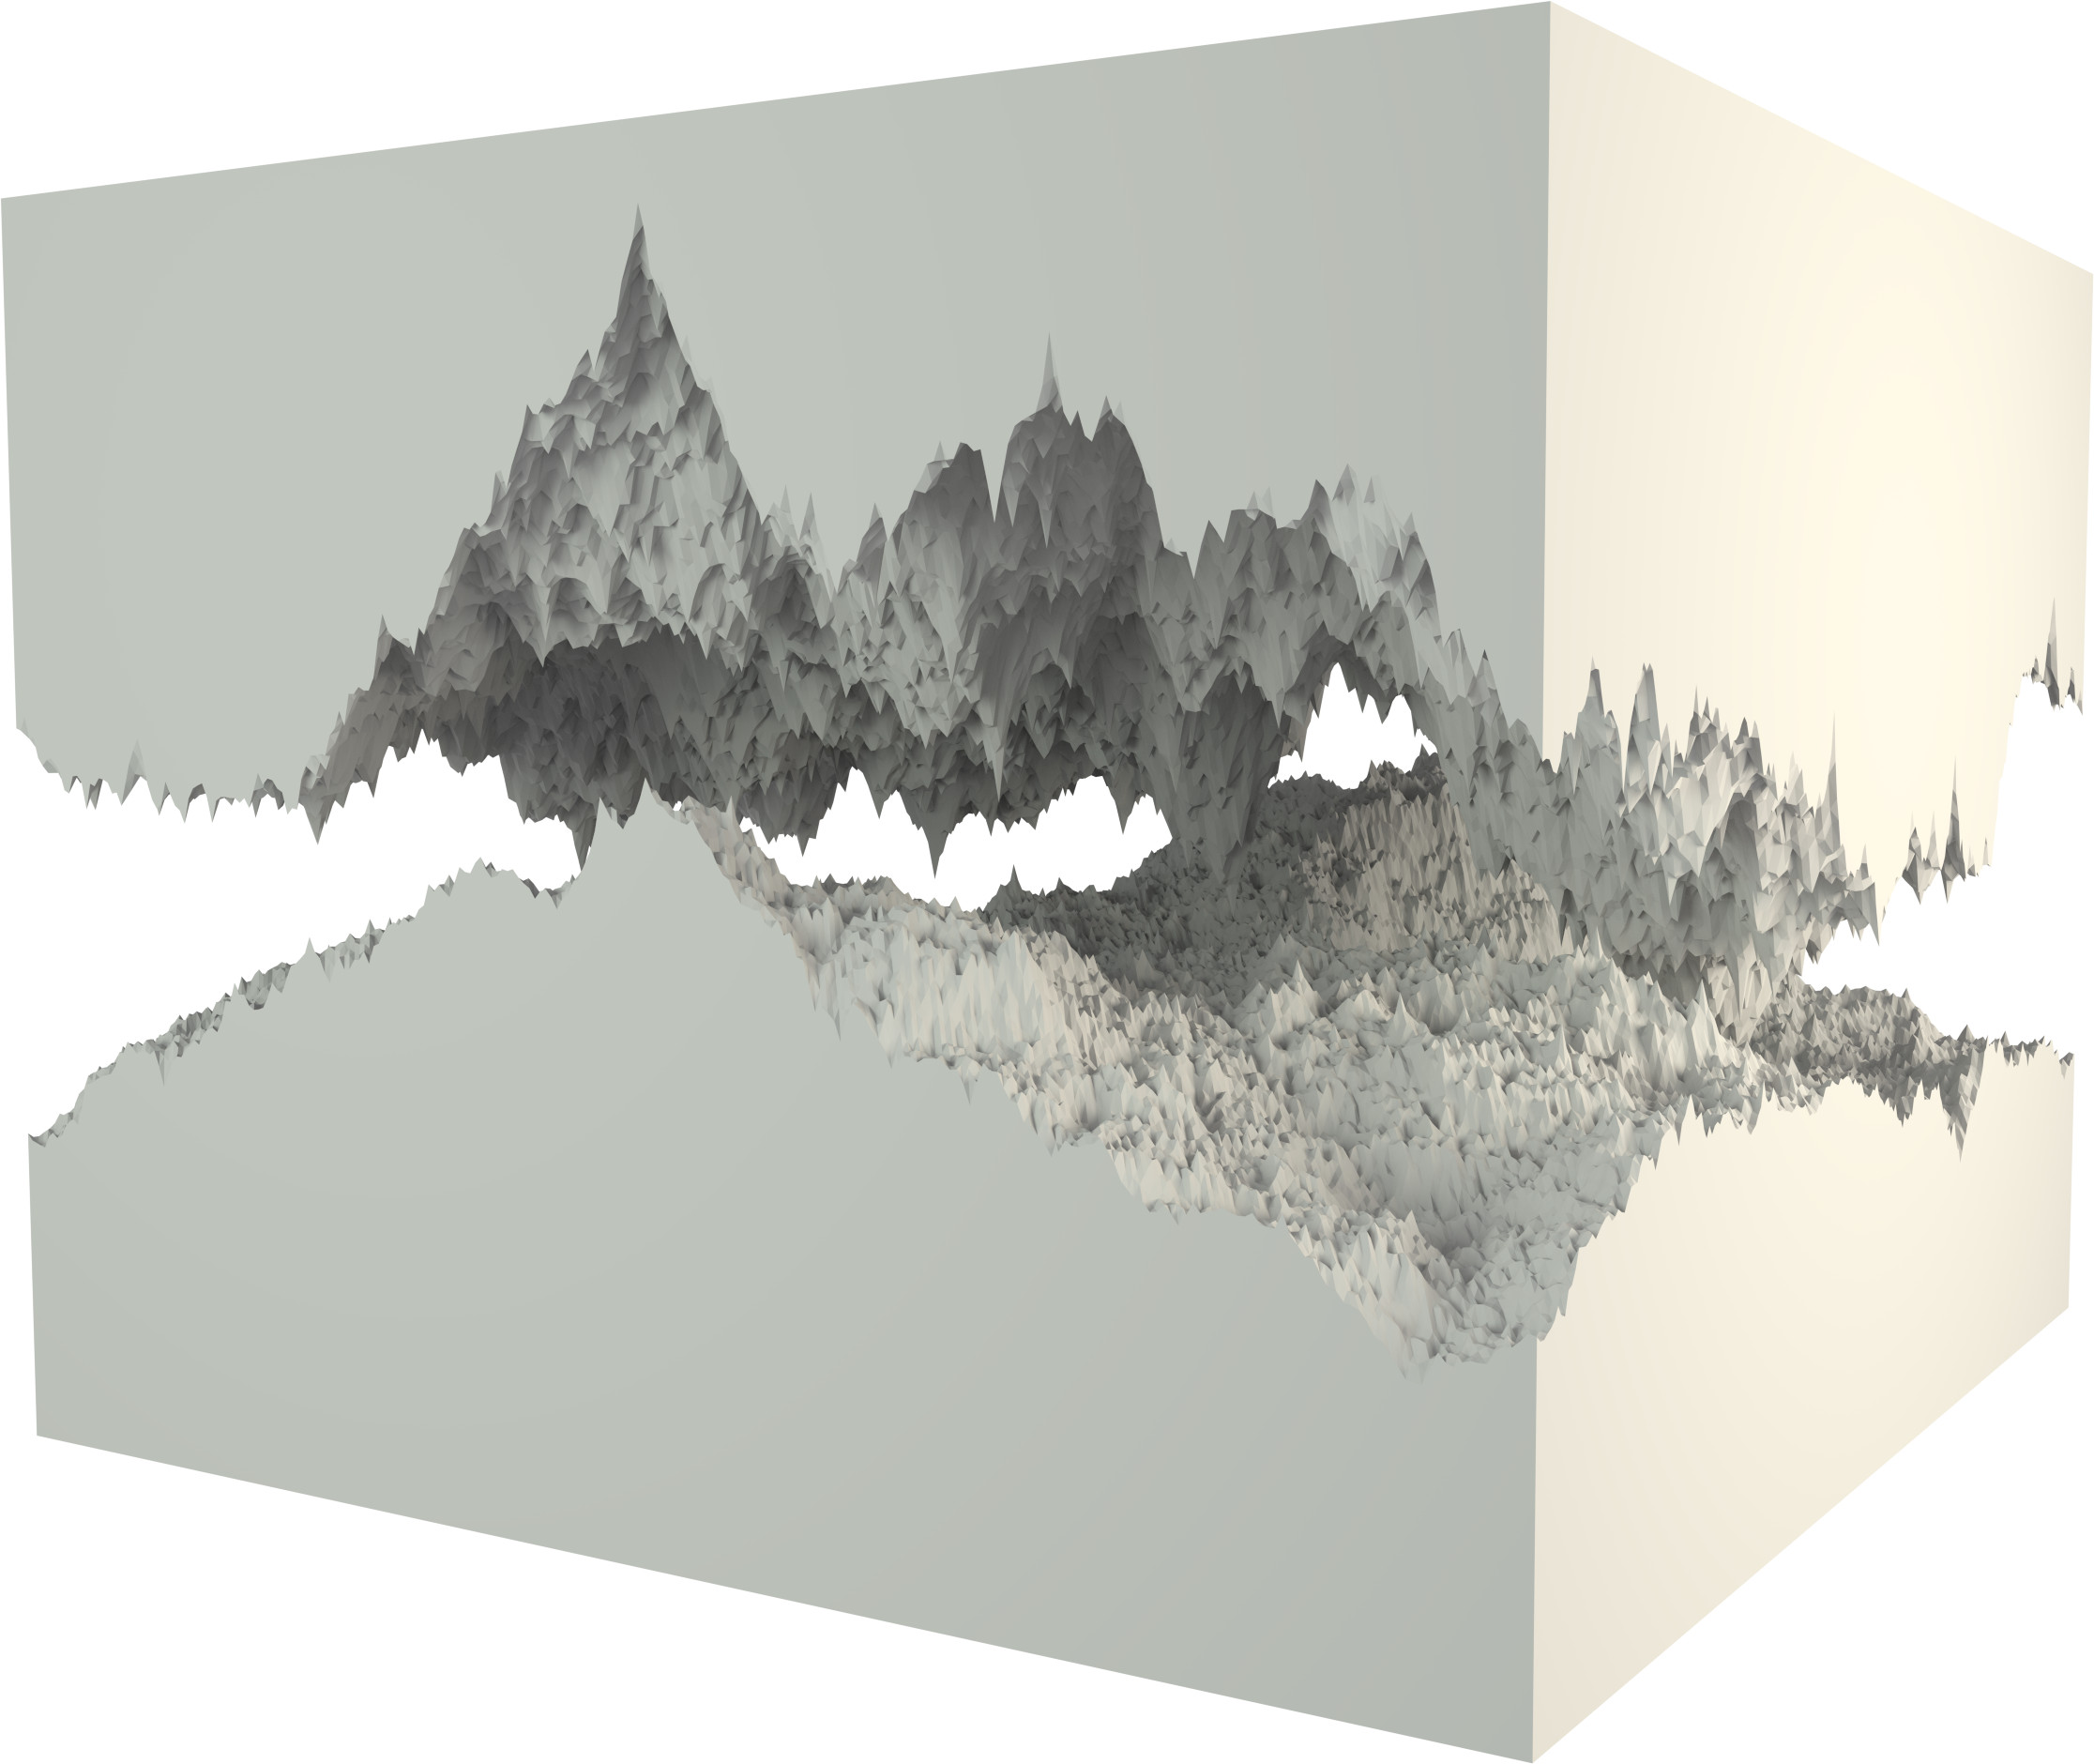
\includegraphics[width=\textwidth]{images/fracture/large_fracture05.jpg}%
    \caption{%
        A randomly generated fracture.%
    }%
\end{figure}%
\vspace{\fill}

\chapter*{Introduction}
\addcontentsline{toc}{chapter}{Introduction}
We want to study the behaviour of water trapped in nanoscale pores and fractures in silica, so need a way to generate and characterize such structures. We choose to model a fracture as two surfaces, with the volume between the surfaces as the void fraction. This makes it easier to make fractures, since we only need to create two surfaces to get a fracture. 

To generate realistic surfaces we could have used scans of the structures we want to simulate, but the problem with this approach is that the resulting fracture will depend a lot on how we interpret the image, and that we can not easily generate a lot of samples of surfaces. To avoid this we use fractals to describe surfaces, and use this to randomly generate surfaces and fractures that are statistically similar to real fractures. Like a lot of phenomena in nature, fractures and surfaces can be very well described by the theory of fractals\cite{mandelbrot1983fractal}, so we think that this method should give good results.

What makes a \emph{fractal} fractal, or what characterizes a fractal, does not have a rigorous definition, but in general a fractal is something that looks similar to itself at different length scales. A fractal might be \emph{identical} to itself at different length-scales (self-similar), or be \emph{statistically similar} to itself (statistically self-similar). In one dimension this looks like \todoao{Examples of 1D, scale x and y equally for self-similar, different scaling for self-affine}

% Fractals and concepts similar to fractals have been discussed as early as the 17th century, but the use of fractals in natural sciences didn't really \hl{take off} before computers became \hl{readily} available and Benoit Mandelbrot gathered and developed a lot of theory on fractals in ``The Fractal Geometry of Nature''\cite{mandelbrot1983fractal}. 

% \todoa{Define fractal dimension}
\todoao{More intro about fractals, some history?}
% \tododone{Define fractal, define self-similarirt and similar terms}

% \todoao{change wording? copied from Fractals...}
% An \emph{affine transformation} transforms a point $\bvec x = (x_1, \dots, x_n)$ into new points $\bvec x' = (r_1x_1, \dots, r_n, x_n)$, where the scaling rations $r_1, \dots, r_n$ are \emph{not} all equal.
% 
% A bounded set $\mathcal{S}$ is \emph{self-affine} if $\mathcal{S}$ is the union of $N$ non-overlapping subsets $\mathcal{S}_1, \dots, \mathcal{S}_N$, each of which is congruent to the set $\bvec r(\mathcal{S})$ obtained from $\mathcal S$ by the affine transform defined by $\bvec r$. Here \emph{congruent} means that the set of points $\mathcal{S}$ is identical to the set of points $\bvec r(\mathcal{S})$ after possible translations and/or rotations of the set\cite{feder1988fractals}.
% 
% A set $\mathcal{S}$ is \emph{statistically self-affine} if $\mathcal{S}$ is the union of $N$ non-overlapping subsets each of which is scaled down by $\bvec r$ from the original, and is identical in all statistical respects to $\bvec r(\mathcal{S})$.
    % \chapter{Fractures}
% \chapter{Introduction}
\vspace*{\fill}
\begin{figure}[hp!]%
\thispagestyle{empty}
    \centering%
    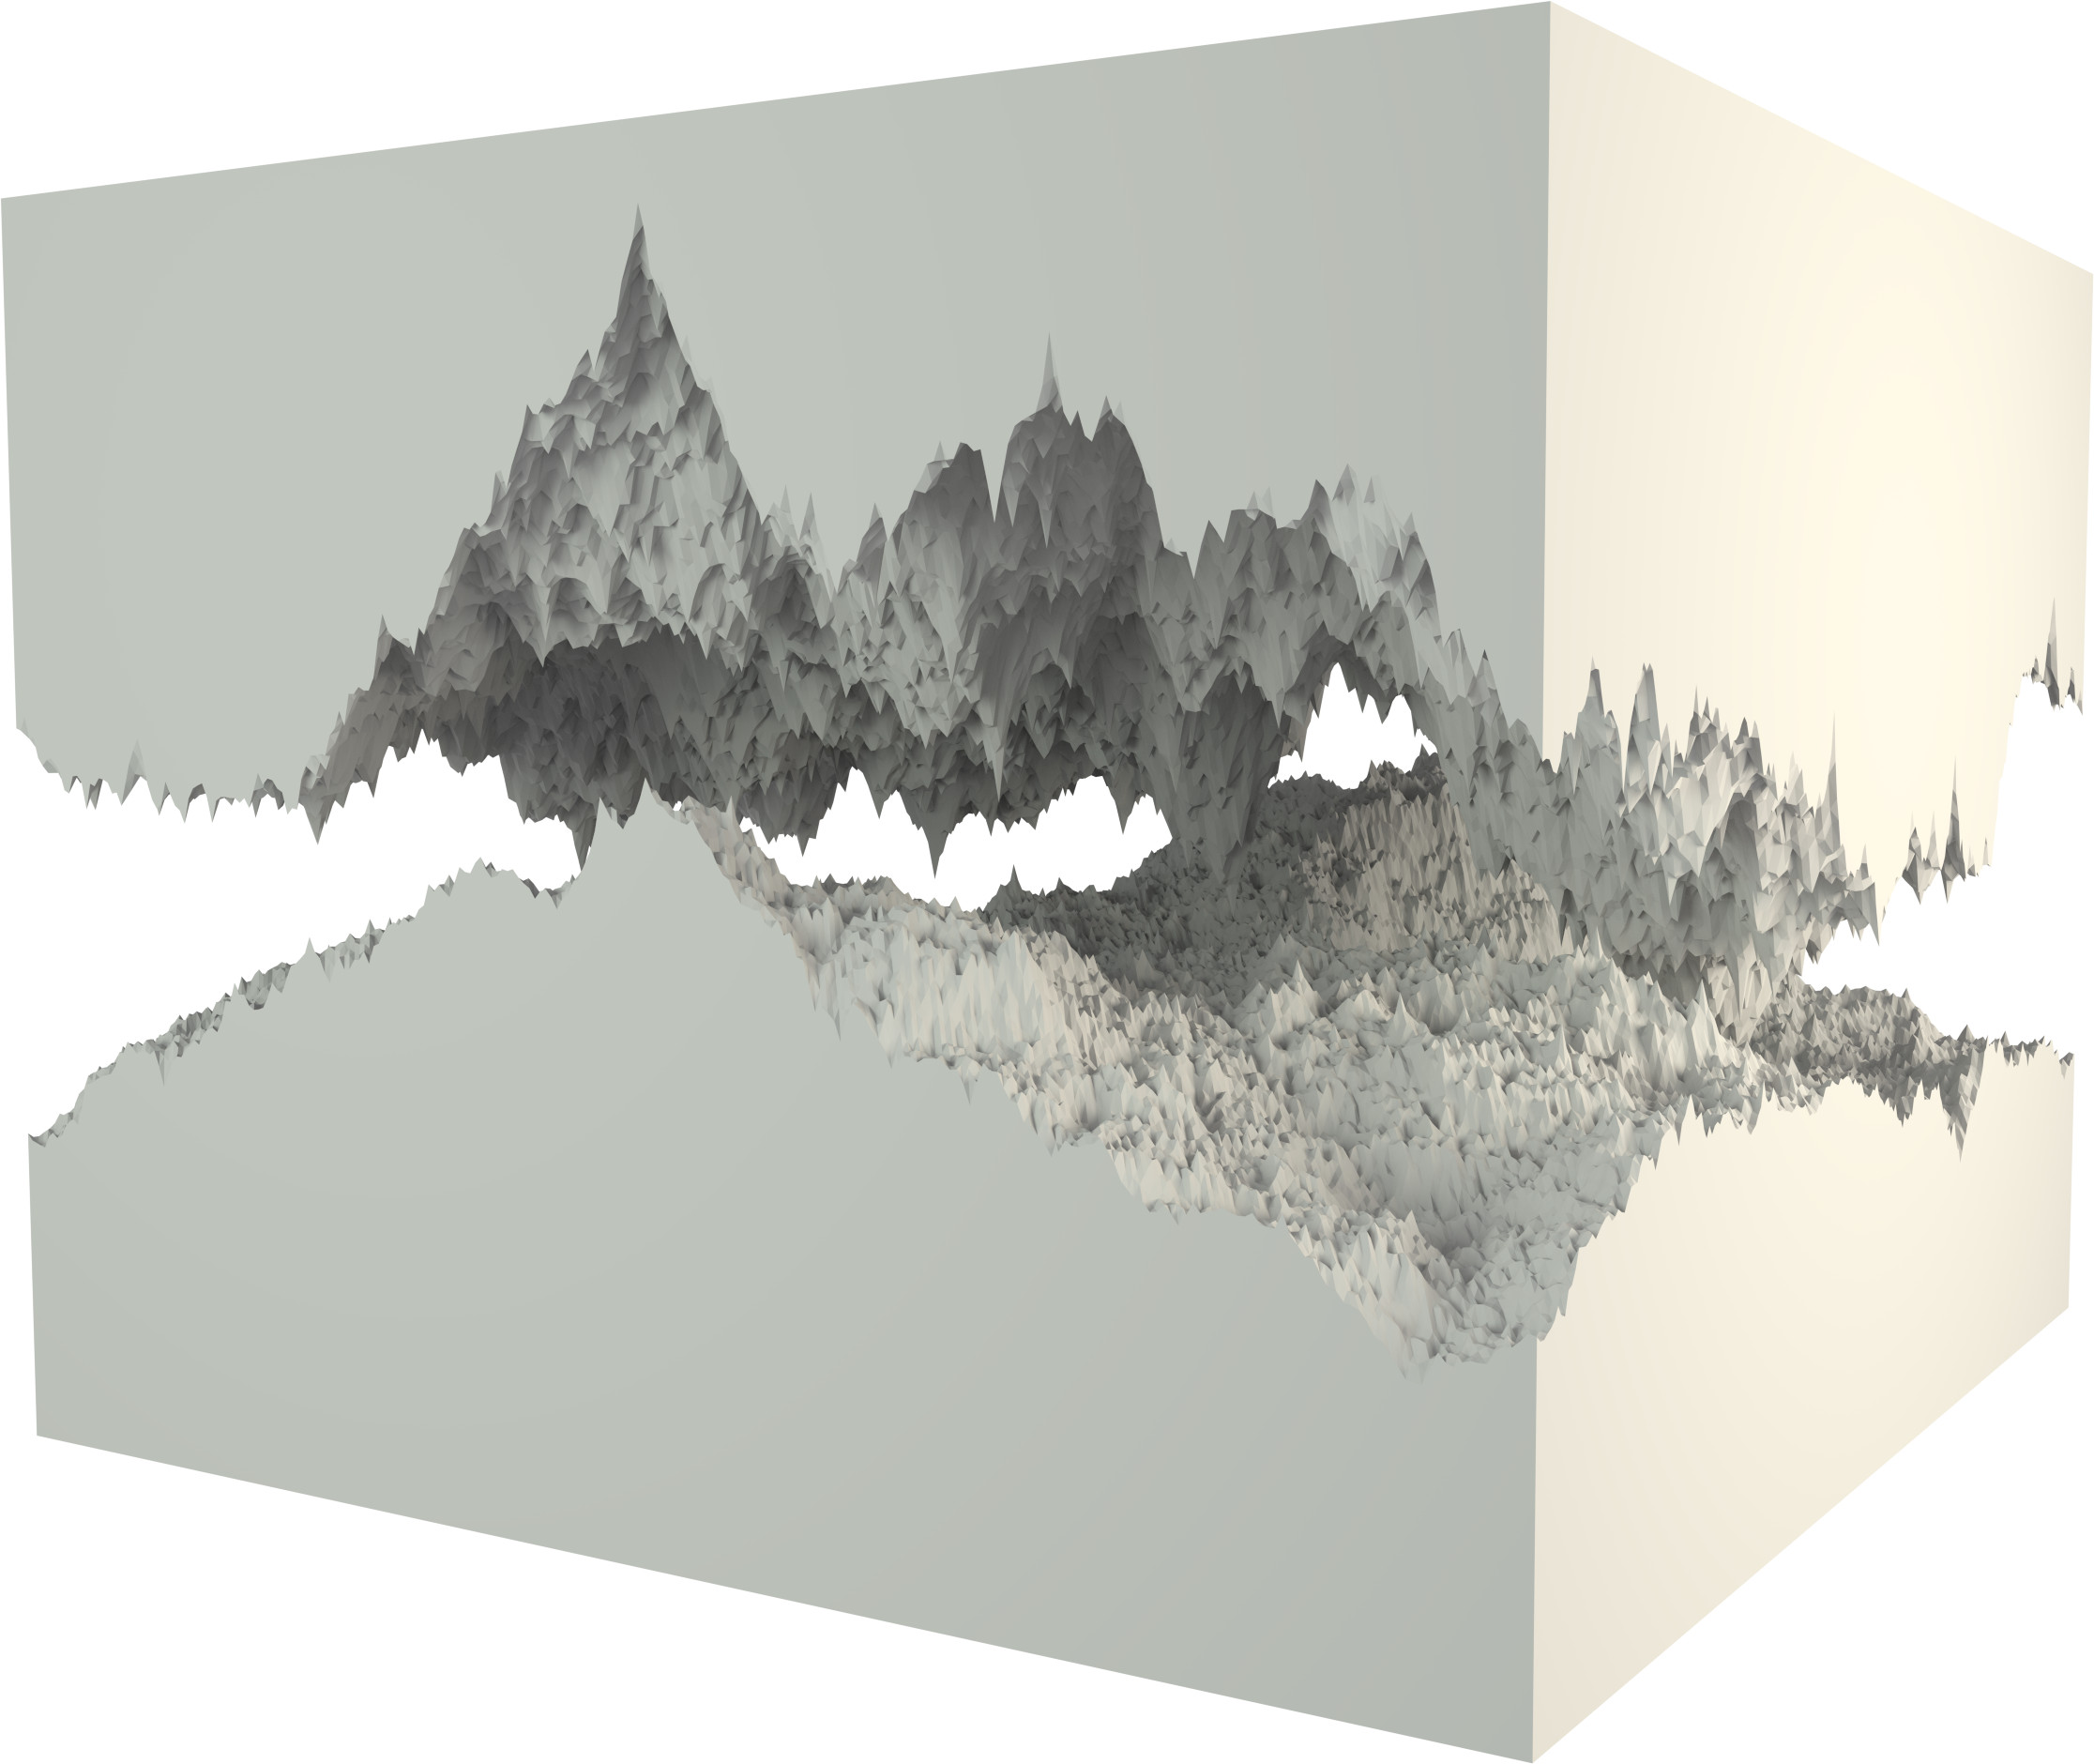
\includegraphics[width=\textwidth]{images/fracture/large_fracture05.jpg}%
    \caption{%
        A randomly generated fracture.%
    }%
\end{figure}%
\vspace{\fill}

\chapter{Introduction}
We want to study the behaviour of water trapped in nanoscale pores and fractures in silica, so need a way to generate and characterize such structures. We choose to model a fracture as two surfaces, with the volume between the surfaces as the void fraction. This makes it easier to make fractures, since we only need to create two surfaces to get a fracture. To generate realistic surfaces we could have used scans of the structures we want to simulate, but the problem with this approach is that the resulting fracture will depend a lot on how we interpret the image, and that we can not easily generate a lot of samples of surfaces. To avoid this we use fractals to describe surfaces, and use this to randomly generate surfaces and fractures that are statistically similar to real fractures. Like a lot of phenomena in nature, fractures and surfaces can be very well described by the theory of fractals\cite{mandelbrot1983fractal}, so we think that this method should give good results.

What makes a \emph{fractal} fractal, or what characterizes a fractal, does not have a rigorous definition, but in general a fractal is something that looks similar to itself at different length scales. A fractal might be \emph{identical} to itself at different length-scales \hl{(self-similar)}, or be \emph{statistically similar} to itself \hl{(statistically self-similar)}. In one dimension this looks like \todoao{Examples of 1D, scale x and y equally for self-similar, different scaling for self-affine}

Fractals and concepts similar to fractals have been discussed as early as the 17th century, but the use of fractals in natural sciences didn't really \hl{take off} before computers became \hl{readily} available and Benoit Mandelbrot gathered and developed a lot of theory on fractals in ``The Fractal Geometry of Nature''\cite{mandelbrot1983fractal}. 

\todoa{Define fractal dimension}
\todoa{More intro about fractals, some history?}
\tododone{Define fractal, define self-similarirt and similar terms}

% \todoao{change wording? copied from Fractals...}
% An \emph{affine transformation} transforms a point $\bvec x = (x_1, \dots, x_n)$ into new points $\bvec x' = (r_1x_1, \dots, r_n, x_n)$, where the scaling rations $r_1, \dots, r_n$ are \emph{not} all equal.
% 
% A bounded set $\mathcal{S}$ is \emph{self-affine} if $\mathcal{S}$ is the union of $N$ non-overlapping subsets $\mathcal{S}_1, \dots, \mathcal{S}_N$, each of which is congruent to the set $\bvec r(\mathcal{S})$ obtained from $\mathcal S$ by the affine transform defined by $\bvec r$. Here \emph{congruent} means that the set of points $\mathcal{S}$ is identical to the set of points $\bvec r(\mathcal{S})$ after possible translations and/or rotations of the set\cite{feder1988fractals}.
% 
% A set $\mathcal{S}$ is \emph{statistically self-affine} if $\mathcal{S}$ is the union of $N$ non-overlapping subsets each of which is scaled down by $\bvec r$ from the original, and is identical in all statistical respects to $\bvec r(\mathcal{S})$.

\chapter{Fractals and fractures}
\todoa{Finish fractals and fractures chapter thing}%
%
% \section{Surface area}
% \section{Distance to nearest atom}
% \begin{itemize}
%     \item Fractals
%     \item Fractional Brownian Motion
%     \item The Hurst Exponent
% \end{itemize}
To generate a fractal surface we use fractional Brownian motion \hl{(fBm)}, introduced by Mandelbrot and van Ness in 1968\cite{mandelbrot1968fractional}. Fractional Brownian motion is a generalization of Brownian motion, which is the random motion of particles suspended in a fluid, which comes from their collisions with the atoms and molecules in the fluid. 

Fractional Brownian motion is a process that generates \hl{data} that \hl{is fractal}, in the sense that it is self-similar%
. The \hl{data} generated by this process can be characterized by a parameter denoted $H$, often called the Hurst exponent. $H$ is related to the \hl{autocorrelation (define?)} of a data set, and is always a number between 0 and 1.
%It is directly related to the fractal dimension $D$ via\cite{feder1988fractals}\todoao{The Hurst exponent relates the root mean square value of the change $dy$ to the distance $x$ over which it changes}
% \begin{align*}
%     D = d - H
% \end{align*}

\hl{The Hurst exponent quantifies the relative tendency of a (time series) to either regress to the mean, or to cluster in a direction.} $H\in[0,0.5]$ indicates a \hl{time series} with long-term switching between high and low values in adjacent pairs, meaning that a single high value will probably be followed by a low value, and vice versa. $H\in[0.5,1.0]$ indicates a \hl{time series} with long-term positive autocorrelation, meaning both that a high value will probably be followed by another high value, and that the values a long time into the future will also tend to be \hl{high (increasing?)}.

Samples of \hl{fBm} with different Hurst parameters will differ in what can quantitatively be called the ``roughness'' or the ``randomness'' of the \hl{series}, as can be seen in \cref{fig:fBm_examples}, where we have plotted some samples of \hl{fBm} with different Hurst exponents.

\todo{in honor of both Harold Edwin Hurst and Ludwig Otto H\"older}

The Hurst exponent and the use of it as a means of characterizing a \hl{dataset/timeseries?} was developed \hl{in the field of hydrology}, as seen in \cite{hurst1951longterm,hurst1965longterm}, where it was used to determine the optimal dam sizing for the Nile river's, by studying the large fluctuations in the flow rate of the river, which there are extensive records of\todoco{rewrite this one-sentence paragraph}. It is denoted $H$ in honor of both Harold Hurst, who was the lead researcher in these studies, and in honor of Otto H\"older \hl{WHY H\"older?}.
%
\todobo{See \cite{mu1988steel} for ref. on fractal dimension of fractured steel surface}%
\todob{No true fractals in nature, since we need infinite resolution. $H = $ Hausdorff dimension? index-$\alpha$?}%
% \todob{Decide on which Hurst figure, and maybe resize the label box in alt. 1? (just increase fig size in plot script)}%
%
\begin{figure}[htpb]%
    \centering%
    {%
%         \newcommand{\s}{\sim}%
        \newcommand{\sa}{H $\approx$ }%
        \includesvg[width=0.8\textwidth, svgpath = ./images/Hurst/]{fbm_1d_examples_grid01}%
    }%
    \caption{%
        Samples of fractional Brownian motion (fBm) with different Hurst exponents, generated using the built-in Matlab function \mono{wfbm}, which uses uses a wavelet-based synthesis method\cite{abry1996wavelet} for generating fBm.%
    }%
    \label{fig:fBm_examples}%
\end{figure}%
% \begin{figure}[htpb]%
%     \centering%
%     \includesvg[width=1.0\textwidth, svgpath = ./images/Hurst/]{fbm_1d_examples}%
%     \caption{}%
% %     \labedl{fig:fBm_examples01}%
% \end{figure}%
%
% We will use fractional Brownian motion (fBm) to 
% We use fractional Brownian motion (fBm) to model fractures 
%
% We will use fractals both for describing, and for generating fractures.
%
% (Several methods of characterizing a fracture could be imagined (\hl{SOURCES, examples}), and we will use several of them.)        
%
% \hl{terrain == heightmap??, finn bra ord her}
%
% \orangebox{
%     \begin{itemize}
%         \item Plot 1D DMA estimate vs. synthesized 1D fBm from FracLab. Difference between with and without new $f^*$.
%         \item Plot 2D DMA estimate vs. synth. 2D fBm from FracLab? \hl{Does FracLab generated 2D?}
%         \item Plot 2D DMA est. vs. input Hurst for diamond square. Compare with and without addition and PBC.
%     \end{itemize}
% }
        \section{Hurst exponent}
One of the earliest methods for measuring the Hurst exponent is a statistical method developed by Hurst in his studies of the Nile river\cite{hurst1965longterm}\cite{hurst1951longterm}. This method is called \emph{rescaled range analysis} and was designed for use on 1-dimensional time series. The method has been generalized to higher dimensions\cite{fan2013rescaled}, but the original 1-dimensional form is shown here.
\todobo{Something about that it's hard to measure, and why.}%

\subsection{Rescaled range analysis}
\todob{Replace rescaled range with $\Delta y \propto \Delta x^H$?}
We have a 1-dimensional time series $f(t)$. The time series is first divided into intervals of length $\tau$. The average over each interval of length $\tau$ is
\begin{align*}
    \langle f \rangle_\tau = \frac{1}{\tau} \sum_{t=1}^\tau f(t).
\end{align*}
We let $F$ be the accumulated deviation from the mean
\begin{align*}
    F(t, \tau) = \sum_{t' = 1}^t \big( f(t') - \langle f \rangle_\tau \big).
\end{align*}
The difference between the maximum and minimum of the accumulated deviation from the mean is the \emph{range} R
\begin{align*}
    R(\tau) = \max_{1 \leq t \leq \tau} \big(F(t,\tau)\big) - \min_{1 \leq t \leq \tau} \big(F(t, \tau)\big).
\end{align*}
The standard deviation $S$ of the time series is estimated using
\begin{align*}
    S^2 = \frac{1}{\tau} \sum_{t=1}^\tau \big( f(t) - \langle f \rangle_\tau \big)^2.
\end{align*}
Hurst found that the observed \emph{rescaled range}, $R/S$, for many time series is described by the empirical relation\cite{feder1988fractals}
\begin{align*}
    \frac{R}{S} = \left(\frac{\tau}{2}\right)^H \sim \tau^H.
\end{align*}
We now see that we can estimate the Hurst exponent by a linear fit of the form
\begin{align*}
    \log \left(\frac{R}{S}\right) \sim H\log\tau,
\end{align*}
where we find $H$ as the slope of the linear fit.



        \section{Detrending moving average\label{sec:dma}}
\todoa{Plot of $\sigma_\text{DMA}^2$ as function of $n$ to determine $H$}
\todobo{Transition from rescaled range to surface?}
To estimate the Hurst exponent of a surface we use a method called detrending moving average (DMA) developed for 1-dimensional data by E. Alessio, A. Carbone et al.\cite{alessio2002dma}, and later generalized to higher dimensions by A. Carbone \cite{carbone2007algorithm}. 

After trying out some different methods for estimating the Hurst exponent, we ended up choosing this method both because it is \hl{easy} to understand and implement, and because it has been shown to give good results, as we will also confirm later. A more detailed comparison of different methods for estimating the Hurst exponent can be seen in\cite{shao2012comparing}, where they find that DMA and DFA (detrended fluctuation analysis) overall perform better than FA (fluctuation analysis), also being less sensitive to the choice of scaling range.%
\todo{good results, easy to implement? }%
\todoao{everything below is for 2/3 D, not always obvious}%

\subsection{Detrending moving average in 2 dimensions}
% We define a \hl{(self-affine)} surface $f(i,j)$, where $f$ is the height in the point $(i,j)$, defined in a discrete 2-dimensional domain with size $N\times N$, for $i,j = 1,\dots,N$. We divide this surface into \emph{overlapping} subsurfaces of size $n \times n$, spanning the whole surface. The \hl{lower left} corners of the surfaces are located in the points $(i,j)$ for $i,j = 1,\dots, N-n+1$ (the limits are set so that the subsurfaces stay within the domain of the surface). In each surface we find a point $(k,l) = (n-m,n-m)$ (relative to lower bottom corner of subsurface)

We define a \hl{(self-affine)} surface $f(i,j)$ of size $N,N$, with $i,j \in [1,N]$. For each point $i,j \in [1,N-n+1]$ in this surface we define a subsurface of size $n\times n$, where each subsurface consists if the points
\begin{align*}
%     (k,l) = \left([i, \dots, i+n], [j, \dots, j+n]\right)%
%     (k,l) = (i,j) + ([1\dots,n], [1,\dots,n])%
%     (k,l) = (i,j) + \left([1\dots,n], [1,\dots,n]\right) \\
    (k,l) \in \left\{ (i,j) + \left([1\dots,n], [1,\dots,n]\right)\right\}
%     (k,l) \in \left( i + [1\dots,n], j + [1,\dots,n]\right)%
\end{align*}
\begin{align*}
    \begin{pmatrix}
        k \\
        l
    \end{pmatrix}
    =
    \begin{pmatrix}
        i \\
        j
    \end{pmatrix}
    +
    \begin{pmatrix}
        1,\dots,n \\
        1,\dots,n
    \end{pmatrix}
\end{align*}%
\todoao{Decide on which vector/matrix thing}%
in the main surface. This means that the point $(i,j)$ is located in the \hl{``lower left''}\todoao{replace lower left with something smart} corner of the subsurface, that the subsurfaces overlap, and that they together span the whole main surface. The limits $i,j \in [1,N-n+1]$ are set so that all subsurfaces are \emph{inside} the main surface.

For each subsurface located at $(i,j)$ we find a point $(k_m, l_m)$ in the subsurface, which can be written as
\begin{align}
%     (k^*, l^*) = (i,j) + (n-m, n-m) %
%     (k_0, l_0) = (i,j) + (n-m, n-m) %
    (k_m, l_m) = (i,j) + (n-m, n-m), %
%     \\
%     \big(i+(n-m), j+(n-m)\big)
    \label{eq:dma_point_in_subsurface}
\end{align}
where $m$ is defined as
\begin{align*}
    &m = \lfloor n\theta \rfloor &\text{for } \theta \in [0,1).
\end{align*}
% With $\theta = 0$ the point is in the upper right corner of the subsurfaces, at $(i+n,i+n)$, for $\theta = 1/2$ the point is in the center, at $(i+n/2, i+n/2)$, and for $\theta \rightarrow 1 \rightarrow (n-1)/n$ the point is in the lower left corner, at $(i,j)$.
The parameter $\theta$ controls the position of this point inside the subsurface, and we have three extreme cases, listed below, and illustrated in \cref{fig:DMA_theta}.%
%
\begin{description}[%
    labelindent=\oldparindent,%
%     leftmargin=12em%
    leftmargin=2.0\oldparindent%
]%
    \item[$\bm{\theta = 0}$:] the point $(k_m, l_m)$ is in the upper right corner of the subsurface, \\at ${(k_m, l_m) = (i+n,i+n)}$
    \item[$\bm{\theta = 1/2}$:] the point $(k_m, l_m)$ is in the center of the subsurface, \\at ${(k_m, l_m) = (i+n/2, i+n/2)}$
    \item[$\bm{\theta \rightarrow 1 \rightarrow (n-1)/n}$:] the point $(k_m, l_m)$ is in the lower left corner of the subsurface, at ${(k_m, l_m) = (i,j)}$
\end{description}%
% \begin{itemize}[label={}]
%     \item $\bm{\theta = 0:}$ the point $(k_m, l_m)$ is in the upper right corner of the subsurface, at $(i+n,j+n)$
%     \item $\bm{\theta = 1/2:}$ the point $(k_m, l_m)$ is in the center, at $(i+n/2, j+n/2)$
%     \item $\bm{\theta \rightarrow 1 \rightarrow (n-1)/n:}$ the point $(k_m, l_m)$ is in the lower left corner, at $(i,j)$
% \end{itemize}
%
\begin{figure}[htpb]%
    \centering%
    \vspace{1em}% Add some space so the figure isn't as close to the content above
    \begin{subfigure}[b]{0.25\textwidth}%
        \includesvg[width=\textwidth, svgpath=./images/Hurst/]{2DDMA_theta04_a}%
%         \caption{Illustration of how to divide a convex hexahedron into five tetraheda.}%
        \caption{$\theta = 0$}%
        \label{fig:DMA_theta_a}%
    \end{subfigure}%
    \hspace{0.1\textwidth}%
    \begin{subfigure}[b]{0.25\textwidth}%
        \includesvg[width=\textwidth, svgpath=./images/Hurst/]{2DDMA_theta04_b}%
%         \caption{A random fracture made from two periodic heightmaps.}%
        \caption{$\theta = 1/2$}%
        \label{fig:DMA_theta_b}%
    \end{subfigure}%
    \hspace{0.1\textwidth}%
    \begin{subfigure}[b]{0.25\textwidth}%
        \includesvg[width=\textwidth, svgpath=./images/Hurst/]{2DDMA_theta04_c}%
%         \caption{A random fracture made from two periodic heightmaps.}%
%         \caption{$\theta \rightarrow 1$ \\ ($\theta = (n-1)/n$)}%
%         \caption{$\theta \rightarrow 1$}%
        \caption{$\theta = (n-1)/n$}%
        \label{fig:DMA_theta_c}%
    \end{subfigure}%
        \caption{%
        Illustration of three extreme cases for the parameter $\theta$ in \hl{2/3} dimensions. The dots are points where the main surface is defined, the red star is the point $(k_m,j_m)$, and the black square marks the subsurface, and the points averaged over to calculate $\bar {f_n}(i,j)$ in \cref{eq:carbone_average}. The illustrations use $n = 3$.%
        \label{fig:DMA_theta}%
    }%
\end{figure}%

We find the average $\bar {f_n}$ of each subsurface \hl{using}
\begin{align}
    \bar {f_n}(i,j) = \frac{1}{n^2} \sum_{k = i}^{i+n} \sum_{l = j}^{j+n} f(k,l),
    \label{eq:carbone_average}
\end{align}
and we define the \emph{generalized variance}, $\sigma_\text{DMA}^2$, as \hl{the sum of the squared differences between} the value in the point $f(k_m,l_m)$ minus the average $\bar {f_n}(i,j)$, for each subsurface. This can be written as
\begin{align}
    \sigma_\text{DMA}^2 
%     &= \frac{1}{(N-n)^2}\sum_{i=n-m}^{N-m} ~ \sum_{j=n-m}^{N-m} 
%     \big(
%         f(i,j) - \tilde f_n(i,j)
%     \big)^2,% \label{eq:dma_variance}
%     \\
    &= \frac{1}{(N-n)^2}\sum_{i=1}^{N-n+1} ~ \sum_{j=1}^{N-n+1} 
    \big(
        f(k_m,j_m) - \bar f_n(i,j)
    \big)^2%
%     \qquad\text{for } k_m, j_m \text{as in \cref{eq:dma_point_in_subsurface}}%
    \nonumber\\%
    &= \frac{1}{(N-n)^2}\sum_{i=1}^{N-n+1} ~ \sum_{j=1}^{N-n+1} 
    \big(
        f(i+n-m,j+n-m) - \bar f_n(i,j)
    \big)^2.
    \label{eq:dma_variance}
\end{align}

It can be shown that this generalized variance has a power-law dependence on $n$ \cite{alessio2002dma,carbone2007algorithm}, which goes as
\begin{align*}
    \sigma_\text{DMA}^2 \sim \left(2n^2\right)^H.
\end{align*}
We can use this dependence to estimate the Hurst exponent $H$, by calculating $\sigma_\text{DMA}^2$ for different sizes of the subsurfaces, $n$. We estimate $H$ by a linear fit of $\log \left(\sigma_\text{DMA}\right)^2$ against $\log \left(2n^2 \right)$, where $H$ is the slope of this fit.

In the paper by Anna Carbone that generalizes DMA to higher dimensions\cite{carbone2007algorithm} they use different parameters for each spatial dimension $d$, $\bvec\theta = \theta_1, \dots, \theta_d$ and $\bvec{n} = n_1, \dots, n_d$, but for simplicity and to avoid \hl{strange/spurious?} results, we use $\theta_1 = \theta_2 = \theta$ and $n_1 = n_2 = n$.

A modification of the method mentioned is replacing $\bar f_n(i,j)$ in \cref{eq:dma_variance} with\todoao{check this equation}
\begin{align*}
    \bar {f_n}^*(i,j) = (1-\alpha) f_n(i,j) + \alpha \bar {f_n}(i-1,j-1),
\end{align*}
where
\[
    \alpha = n^2/(n+1)^2,
\]
and $\tilde f_n(i,j)$ has the same form as before (see \cref{eq:carbone_average}). To use this modification we also have to change the limits in \cref{eq:dma_variance} from ${i,j\in [1,N-n+1]}$ to $i,j\in [2,N-n+1]$. This modification has been shown to give better results for small systems\cite{carbone2007algorithm}\todo{why?}, and since we are usually generating surfaces with a \hl{resolution/$N$ of 100-200}, we use this modified method in our implementation of the method. \todo{maybe implement both methods?}

\todob{The method is implemented in Matlab/Octave}

\subsection{The performance of detrending moving average}
\todoa{Read through DMA performance, make some conclusions from plot}
To verify that the method we used for estimating the Hurst exponent worked as intended, and gave good results, we ran a series of tests using synthetic \hl{(1D)} time series and \hl{(2D)} surfaces \hl{of fractional Brownian motion} with a known Hurst exponent. When doing these tests we soon realized that a big problem with synthesizing time series and surfaces with a given Hurst exponent is that it's both hard to accurately measure the exponent, and it's hard to synthesize data with a given exponent. \hl{This means that when testing methods for analysing and synthesizing signals, you never know if it's you measuring method, or your synthesizing method that is causing problems if things aren't working as intended.}

To test the \hl{DMA method} we synthesized data with a given Hurst exponent using 4 different \hl{methods/programs}, and measured the exponent using the detrending moving average method for each of these methods. 

For synthesizing 1D data we used the built-in Matlab-function \hl{cite matlab?} \Verb!wfbm! which uses a wavelet-based synthesis method described by Abry and Sellan \cite{abry1996wavelet}, and two methods from the Matlab-toolbox FracLab\cite{fraclab_toolbox}, \Verb!fbmwoodchan! which uses a method proposed by Wood and Chan in \cite{wood1994simulation}, and \Verb!fbmlevinson! which uses Cholesky/Levinson factorization from \cite{levinson1947wiener}. 

There are many methods and algorithms for generating \hl{2D/3D/surfaces} data with a given Hurst exponent, but we had problems finding working implementations of any of them. We will later implement a midpoint displacement method for this (see \cref{chap:generating_surfaces,subsec:SRA_implementation}), but having external reference is very useful, so we used a function from FracLab called \Verb!synth2!, which, according to the documentation of the function:%
\begin{quote}
    \textit{Generates a 2D Fractional Brownian Motion (fBm) using an incremental Fourier Method for processes with stationary increments of order (0,1) and (1,0).}
\end{quote}\todobo{No sources are given in FracLab documentation...}
We will later also test our own implementation of a method for generating \hl{2d/3d} data against \hl{DMA}.
% ``Generates a 2D Fractional Brownian Motion (fBm) using an incremental Fourier Method for processes with stationary increments of order (0,1) and (1,0)''.

See \cref{fig:dma_performace} for a plot of Hurst exponent measured using \hl{DMA} as a function of the exponent used as input for the four different methods for generating synthetic data above, for three different values of the parameter $\theta$.

From \cref{fig:dma_performace} we conclude that $\theta = 0.0$ seems to give the best and most consistent results, as also noted by Gao-Feng Gu and Wei-Xing Zhou in\cite{gu2010detrending}, where they further develop the \hl{DMA} method to analyse multifractals. \hl{We would liked to have more 2D data references.}%
\todob{Fix newcommand stuff in \cref{fig:dma_performace}, and maybe legend texts (can remove stuff now that we know have smaller text in figures)}
%
\begin{figure}[htpb]%
    \centering%
    {
        \newcommand{\f}{\footnotesize}%
        \newcommand{\x}{\text}%
        \newcommand{\thislabelaaaaaa}{{\f $H_\x{in}=H_\x{out}$}}%
        \includesvg[width=1.0\textwidth, svgpath=./images/diamond_square_Hurst/test_HDDMA/]{fig03}%
    }
%     \caption[
%         Plot of the Hurst exponent as estimated by the detrending moving average method, used on data from four different synthetic signals, against the exponent used as input when generating the signals, and for three different values of the parameter $\theta$ used in \hl{DMA}. All methods except synth2 generate 1-dimensional signals, while synth2 generates a 2-dimensional signal. \hl{FINISH CAPTION}. %
%     ]{%
%         Plot of the Hurst exponent as estimated by the detrending moving average method, used on data from four different synthetic signals, against the exponent used as input when generating the signals, and for three different values of the parameter $\theta$ used in \hl{DMA}. All methods except \Verb!synth2! generate 1-dimensional signals, while \mono{synth2} generates a 2-dimensional signal. \hl{FINISH CAPTION}. %
%         \label{fig:dma_performace}%
%     }%
    \caption{%
        Plot of the Hurst exponent against the exponent used as input when generating the signals, as estimated by the detrending moving average method, used on data from four different synthetic signals, and for three different values of the parameter $\theta$ used in \hl{DMA}. For the 1d methods we have averaged over 1000 samples for each point, and for \mono{synth2} we have averaged over 100 samples, for input Hurst exponents between 0.05 and 0.95 in steps of 0.1. All methods except \mono{synth2} generate 1-dimensional signals, while \mono{synth2} generates a 2-dimensional signal. \hl{FINISH CAPTION}. %
        \label{fig:dma_performace}%
    }%
\end{figure}%

\orangebox{
    \begin{itemize}
        \item 1D: Plot of H from DMA vs. input H for wfbm (Matlab built in), and perhaps a FracLab variant?
        \item 1D: Plot of H from DMA vs. H from FracLab measure method?
        \item 2D: Plot of H from DMA vs. input DiamondSquare H and vs. synth2? (this could fit better in diamondsquare part).
    \end{itemize}
}

    \chapter{Generating surfaces}
\hl{Stuff to define?}
\begin{itemize}
    \item fBm surfaces
    \item Hurst exponent
    \item Gaussian random variable ?
    \item non-stationary
    \item self-similar
    \item isotropic
    \item lacunarity
\end{itemize}

Introduction?
% When generating random surfaces we want to be able to control the properties like the Hurst exponent (\hl{etc.?}) of the surface.

To generate our random surfaces we use an iterative midpoint displacement method usually called successive random additions \hl{(SRA)}. The method is based on a method proposed by Fourner in 1982\cite{fournier1982computer}, but with some modifications suggested by Voss\cite{voss1985random, voss1988fractals}. The method has further been discussed by Saupe\cite{saupe1988algorithms}, amongst others. We choose this method mainly because it's possible to generate periodic surfaces with it, because it generates very good approximations to fBm surfaces\cite{zhou2005comparison}, and because the Hurst exponent of the generated surfaces is easy to control. The method is also easy to understand, easy to implement, and generates surfaces with high resolution very fast. The method is widely used in scientific applications\hl{cite??} because of these properties, and is also used for generating surfaces in computer graphics, since the surfaces look very realistic \hl{with only some minor artefacts?? (high, narrow peaks)}.

\section{Midpoint displacement methods (in 1 dimension)}
\todo[inline]{The most basic method we used is a very basic but widely used method, which has many variations and names. The most common names are ``the diamond-square algorithm''\hl{cite}, ``the midpoint displacement method''\hl{cite}, ``plasma fractal'' and ``cloud fractal''.}

The method we use to generate random surfaces is very similar to the standard midpoint displacement method, which in 1 dimension goes as follows. See \cref{fig:midpoint01} for a visual presentation.
%
\begin{enumerate}
    \item Give the values at the endpoints of the interval, $y_0$ and $y_n$, random values from a Gaussian random variable with mean $\mu = 0$ and variance $\sigma_0^2$. This initial standard deviation $\sigma_0$ can be chosen freely.
    \item Generate the value in the center of the interval, $y_{n/2}$, by averaging over the two endpoints and adding a Gaussian random number with mean $\mu = 0$ and a \emph{reduced} variance
    \begin{align}
         \sigma_1^2 = \left(1/2\right)^{2H}\sigma_0^2, \label{eq:midpoint_sigma_first}
    \end{align}
    where $H$ is the wanted Hurst exponent.
    \item Continue generating the values in the center of each sub-interval until you reach the desired number of points, while reducing the variance of the random number by a factor $\frac{1}{2}$ each iteration\todo{Why 1/2? (needed to create good approx. to fBm, see \cite{voss1985random})}. For iteration $i$ we have
    \begin{align}
        \sigma_i^2 = \left(1/2\right)^{i2H}\sigma_0^2. \label{eq:midpoint_sigma_general}
    \end{align}
\end{enumerate}
%
\begin{figure}[htpb]%
    \centering%
    \includesvg[width=0.5\textwidth, svgpath=./images/diamond_square/]{random_midpoint_displacement_regular02}%
    \caption{%
        \hl{Illustration of the midpoint displacement method in 1 dimension. We increase the number of points from 2 to 9 using 3 iterations.}%
        \label{fig:midpoint01}%
    }%
\end{figure}%

This method generates a \hl{1-dimensional line}, with a Hurst exponent \hl{close} to the input $H$\todo{how close?}. But since we only add random numbers to the new values, the result is non-stationary for $H \neq 0.5$\cite{voss1985random}\hl{, and it is neither self-similar or isotropic, as noted by Mandelbrot}\cite{mandelbrot1982comment}. To mitigate this we implement the addition suggested by Voss\cite{voss1985random}, which consists of adding a random number to \emph{all} points in each iteration, both the new and old. Voss called this modified method \emph{successive random additions}.

\section{Successive random additions in 2 dimensions}
As mentioned \st{before}, the method called \emph{successive random additions} is a modification of the regular midpoint displacement method first described by Richard F. Voss\cite{voss1985random}, where we add random numbers to \emph{all} points in each iteration, compared to just the \emph{new} points in the regular midpoint displacement method. This modification means that we can replace the factor $(1/2)$ in \cref{eq:midpoint_sigma_first,eq:midpoint_sigma_general} with a general factor $r$\todo{why? (something about distance between points)}, and we get
\begin{align*}
    \sigma_i^2 = r^{2H}\sigma^2_{i-1}.
\end{align*}
\hl{$r$ controls the lacunarity/roughness, $H$ independent of $r$}

% \subsection{(on an infinite grid) in 2 dimensions}
\subsection{On an infinite grid}
Voss has geneneralized the the method of successive random additions to higher dimensions\cite{voss1985random}, and this generalized form is the algorithm we use when generating fractures. We generate surfaces in the form of heightmaps, meaning a 2-dimensional grid of points ({$x,y$}), with a value for the height in each point \hl{($z(x,y) = z_{x,y}$)} which is generated by the algorithm.

The central part of the algorithm consists of two steps often called the \emph{diamond-step} and the \emph{square-step}. We start with a simple case of an infinite grid of evenly spaced points, all with known $z$-values. The two steps are as follows:
\begin{description}
    \item[The \emph{square-step}:] The grid can be divided into small squares consisting of four points in each square, as in the leftmost square in \cref{fig:simple_square_step}. We generate the $z$-value in the center of each of these squares by averaging the $z$-values of the four corners of each square, as indicated by the red dots and arrows in \cref{fig:simple_square_step}. Then add a random Gaussian number with mean $\mu = 0$ and variance $\sigma_i^2 = \sigma_{i-1}^2r^{2H}$ to all new and old points, where $\sigma_{i-1}^2$ is the variance used in the last step of the algorithm.
    \label{enum:test}
    
    \item[The \emph{diamond-step}:] After the square-step the grid can be divided into smaller squares that are tilded by 45 degrees, as in the leftmost square in \cref{fig:simple_diamond_step}. We generate the $z$-values in the center of each square by averaging the $z$-values of the four corners of each square, as indicated by the red dots and arrows in \cref{fig:simple_diamond_step}. We then add a random Gaussian number with mean $\mu = 0$ and variance $\sigma_{i+1}^2 = \sigma_i^2r^{2H}$, to all new and old points. 
\end{description}
See \cref{fig:diamond_square_applied} for an illustration of the algorithm applied once on a larger grid. 

\begin{figure}[htpb]%
\centering%
%
\setlength{\myfigwidth}{0.5\textwidth}%
\setlength{\mycaptionwidth}{0.3\textwidth}%
%
% \parbox[c][2cm][c]{\myfigwidth}{
%     \includesvg[width=\myfigwidth, svgpath = images/diamond_square/]{simple_square_step_solarized08}
% }
% \parbox[c][2cm][c]{\mycaptionwidth}{
%     \subcaption{Square-step}
%     \label{fig:simple_square_step}
% }
%
% \begin{minipage}[c][2cm][c]{\myfigwidth}
%     \includesvg[height=2cm, svgpath = images/diamond_square/]{simple_square_step_solarized08}
% \end{minipage}
% \begin{minipage}[c][2cm][c]{\mycaptionwidth}
%     \subcaption{Square-step}
%     \label{fig:simple_square_step}
% \end{minipage}
%
\begin{minipage}[c]{\myfigwidth}%
    \includesvg[width=\textwidth, svgpath = images/diamond_square/]{simple_square_step_solarized08}%
\end{minipage}%
\begin{minipage}[c]{\mycaptionwidth}%
    \subcaption{Square-step}%
    \label{fig:simple_square_step}%
\end{minipage}%
\\%
\vspace{2mm}%
\begin{minipage}[c]{\myfigwidth}%
    \includesvg[width=\textwidth, svgpath = images/diamond_square/]{simple_diamond_step_solarized05}%
\end{minipage}%
\begin{minipage}[c]{\mycaptionwidth}%
    \subcaption{Diamond-step}%
    \label{fig:simple_diamond_step}%
\end{minipage}%
%
\caption{Illustration of the two steps used in the diamond square algorithm for generating random surfaces. The grey points are old points, the black points are new points, and the red points are the points used in the calcuation of the averages when generating the new points.}%
\label{fig:diamond_square_steps}%
\end{figure}%

We see that by first applying the square-step and then applying the diamond-step, we add one point in between each point in each direction, almost doubling the resolution of the grid. In general we go from $n$ to $n + (n-1)$ points in each direction. By applying the algorithm several times we get \todo{replace $n$ with $N$ and $i$ with $n$?}
\begin{align}
    n_1 &= n_0 + (n_0-1) = 2n - 1 \nonumber\\
    n_2 &= 2n_1 - 1 = 4n_0 - 3 \nonumber\\
    n_3 &= 2n_2 - 1 = 9n_0 - 7 \nonumber\\
    &\vdotswithin{=} \nonumber\\
%     &\shortvdotswithin{=}
    n_i &= 2^i(n_0-1) + 1, \label{eq:diamond_step_resolution}
\end{align}
where $i$ is the number of times we have applied the algorithm. This means that using the diamond-square algorithm we can go from any resolution $n_0$ to all resolutions satisfying $n_i = 2^i(n_0 - 1) + 1$.
%
\begin{figure}[htpb]%
    \centering%
    \includesvg[width=0.7\textwidth, svgpath = images/diamond_square/]{increase_resolution_solarized_starssquares03}%
    \caption{%
        The diamond-square algorithm applied once on a grid of $3\times 3$ points, increasing the number of points from 9 to 25. The orange square points are generated by the square-step (see \cref{fig:simple_square_step}), and the blue star-shaped points by the diamond-step (see \cref{fig:simple_diamond_step}).%
    }%
    \label{fig:diamond_square_applied}%
\end{figure}%

% \subsection{Successive random additions on a finite grid (in 2 dimensions)}
\subsection{On a finite grid}
Since we are using computers to generate our surfaces, which have limited memory, we can't use infinite grids. This means we get some special cases that needs to be taken care of when generating points near the edges of the grid.\todo{transition to below}

For the square step we generate one new point in the center each square formed by the grid from the previous iteration, and in general we generate the $z$-values in the points
\begin{align}
    &\left(x_{i+1/2}, y_{j+1/2}\right) &0\leq i,j < n, \label{eq:square_step_limits}
\end{align}
where $(x_i,x_j)$ are the points in the grid after the last iteration. In general the averages we calculate for the new points can be written as\todo{make this equation nicer}
% \begin{align}
%     (x_{i+1/2}, y_{j+1/2}) 
%     &= \frac{1}{4}\big(
%         (x_i, y_j) + (x_{i+1}, y_j)\nonumber\\
%         &+ (x_i, y_{j+1}) + (x_{i+1}, y_{j+1})
%     \big)
%     &0\leq i,j < n.
%     \label{eq:square_step}
% \end{align}
\begin{align}
    (x_{i+1/2}, y_{j+1/2}) 
    = \frac{1}{4}\big[
        (x_i, y_j) + (x_{i+1}, y_j)
        &+ (x_i, y_{j+1}) + (x_{i+1}, y_{j+1})
    \big],
    \label{eq:square_step}
\end{align}
using the limits in \cref{eq:square_step_limits}. We see that the square-step only uses points inside the grid, which means that we don't have to modify it when going to a finite grid.

For the diamond-step we generate the values in the points

\begin{align}
    &(x_{i+1/2}, y_j) &\text{for } 0\leq i<n \text{ and } 0\leq j \leq n& \label{eq:diamond_step_limits01}\\
    &(x_i, y_{j+1/2}) &\text{for } 0\leq i\leq n \text{ and } 0\leq j < n&. \label{eq:diamond_step_limits02}
\end{align}
In general the averages we calculate for the new points can be written as\todo{make these equations nicer}
% \begin{align}
%     (x_{i+1/2}, y_j) 
%     &= 
%     \frac{1}{4}\big(
%         (x_i, y_j) + (x_{i+1}, y_j) + (x_{i+1/2}, y_{j-1/2}) + (x_{i+1/2}, y_{j+1/2})
%     \big) \label{eq:diamond_step01}\\
%     (x_i, y_{j+1/2}) 
%     &= 
%     \frac{1}{4}\big(
%         (x_i, y_j) + (x_i, y_{j+1}) + (x_{i-1/2}, y_{j+1/2}) + (x_{i+1/2}, y_{j+1/2})
%     \big). \label{eq:diamond_step02}
% \end{align}
\begin{align}
    (x_{i+1/2}, y_j) 
    &= 
    \frac{1}{4}\big[
        (x_i, y_j) + (x_{i+1}, y_j) \nonumber\\
        &+ (x_{i+1/2}, y_{j-1/2}) + (x_{i+1/2}, y_{j+1/2})
    \big]
    \label{eq:diamond_step01}\\
    (x_i, y_{j+1/2}) 
    &= 
    \frac{1}{4}\big[
        (x_i, y_j) + (x_i, y_{j+1}) \nonumber\\
        &+ (x_{i-1/2}, y_{j+1/2}) + (x_{i+1/2}, y_{j+1/2})
    \big],
    \label{eq:diamond_step02}
\end{align}
using the limits in \cref{eq:diamond_step_limits01,eq:diamond_step_limits02}. We now see that when generating points near the edges using the diamond-step, specifically when generating the points $(x_{i+1/2}, y_j)$ for $j \in \{0, n\}$ and $(x_i, y_{j+1/2})$ for $i = \{0, n\}$, we need to average over points that lie outside the grid. There are two possible solutions, depending on the surface we are generating. If generating a periodic surface, the solution is to wrap around the edges using periodic boundary conditions, and find the point we need on the opposite side of the grid. For example (using $i = j = 0$)
\begin{align*}
    (x_{1/2}, y_{-1/2}) = (x_{1/2}, y_{n-1/2}).
\end{align*}
If generating a non-periodic grid we simply ignore the points that lie outside the grid when calculating the averages, and just use the \hl{three/3} other points.

% \subsection{Implementing successive random additions (on a finite grid in 2 dimensions)}
\subsection{Implementation}
In our implementation we generate a surface on a finite grid of size $N\times N$, starting with only the $z$-values in the four corners defined, giving a resolution $n_0 = 2$. As shown in \cref{eq:diamond_step_resolution} the algorithm can go from any resolution $n_0$ to any resolution \hl{of the form} $n_p = 2^p(n_0-1) + 1$ by applying the algorithm $p$ times, which means that our implementation can generate surfaces with resolutions
\begin{align*}
    N &= 2^p(2-1) + 1 = 2^p + 1,
\end{align*}
where $p$ is any positive integer.

We implement generation of both periodic and non-periodic surfaces using using \crefrange{eq:square_step_limits}{eq:diamond_step02}, while skipping points outside the grid for non-periodic surfaces, and wrapping around the edges using periodic boundary conditions when generating periodic surfaces.

To ensure that the periodic surfaces actually turn out periodic we start with all four corners having the same value. We also let the right and bottom edge be equivalent to the left and top edge, respectively, which effectively means that all four corners should always have the same $z$-value. To ensure that the opposite edges stay equal to each other we never generate any points on the right and bottom edge, but just copy the $z$-values from the opposite \hl{corresponding} edge after the diamond-step.

This leaves us with the following algorithm for generating a surface which approximates a 2-dimensional fractional Brownian motion with Hurst exponent $H$
\begin{enumerate}
    % \itemsep1pt \parskip0pt \parsep0pt
    \renewcommand{\labelitemii}{$\bullet$}
    
    \item Allocate a grid of size $N\times N$, where $N = 2^p + 1$, and $p$ is any positive integer. \hl{This grid will store the $z$-values, or the height of the surface, in each grid point $(x,y)$.}

    \item Initialize the $z$-values of the corners of the grid by drawing random numbers from a Gaussian distribution with mean $\mu = 0$ and variance $\sigma_0$. The initial variance can be chosen freely. \hl{The initial resolution is now $n_0\times n_0$, with $n = 2$}.
    \begin{itemize}
        \item If generating a periodic surface, give all four corners the same $z$-value.
    \end{itemize}
    
    \item Apply the square-step using \cref{eq:square_step_limits,eq:square_step}. Add a random Gaussian number with mean $\mu = 0$ and variance $\sigma_i = \sigma_{i-1}^2r^{2H}$ to all new and old points.
    \label{enum:square_step}

    \item Apply the diamond-step using \crefrange{eq:diamond_step01}{eq:diamond_step02}. Add a random Gaussian number with mean $\mu = 0$ and variance $\sigma_{i+1} = \sigma_i^2r^{2H}$ to all new and old points.
    \label{enum:diamond_step}
    
    \begin{itemize}
        \item If generating a periodic surface, skip generating $z$-values for points on the right and bottom edge using the diamond-step, and instead copy the values from the opposite edges after the diamond-step.
    \end{itemize}
    
    \item Repeat step \ref{enum:square_step} and \ref{enum:diamond_step} $p$ times until you reach the desired resolution of $N\times N$, where $N = 2^p + 1$. For step $i$ the variance of the random Gaussian numbers is
    \begin{align*}
        \sigma_i^2 = \sigma_0^2(r^i)^{2H}.
    \end{align*}
\end{enumerate}

See \cref{fig:diamond_square_surface} for a surface generated by the algorithm.
%
% \begin{figure}[htpb]%
%     \centering%
%     \includesvg[width=0.7\textwidth, svgpath=./images/diamond_square/surface_example/]{surface_labels}%
%     \caption{%
%         Caption.%
%         \label{fig:diamond_square_surface}%
%     }%
% \end{figure}%
\begin{figure}[htpb]%
    \centering%
    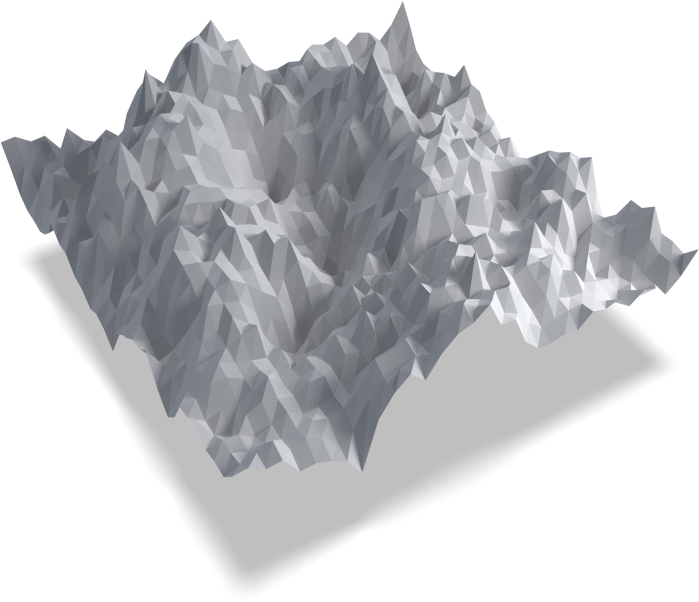
\includegraphics[width=0.5\textwidth]{./images/diamond_square/surface_blender/surface_composite01_cropped.png}%
    \caption{%
        Caption.%
        \label{fig:diamond_square_surface}%
    }%
\end{figure}%

\orangebox{
{\bf Notes:}
\begin{itemize}
    \item Implementation (in Matlab/C++)?
    \item periodic and non-periodic
    \item Mention that DS can be used to increase resolution of any surface
    \item Can increase resolution of generated surface, if we know the seed
\end{itemize}

{\bf Stuff to define:}
\begin{itemize}
    \item Periodic/non-periodic
    \item Lacunarity
\end{itemize}
}

\subsection{Testing the method}
%
\begin{figure}[htpb]%
    \centering%
    {
        \newcommand{\f}{\footnotesize}%
        \newcommand{\x}{\text}%
        \newcommand{\hh}{{\f $H_\x{in}=H_\x{out}$}}%
        \includesvg[width=0.7\textwidth, svgpath=./images/diamond_square_Hurst/test_diamondSquare/]{fig}%
    }
    \caption{%
        Diamond square accuracy? Measured using DMA. The dashed grey line indicates a measured Hurst exponent of 0.75, the solid grey line a measured exponent exactly equal to the input exponent. The green lines are surfaces created using periodic boundary conditions (PBC), the red lines using non-periodic boundaries, the dashed lines using successive random additions (SRA), and the solid lines using the regular midpoint displacement method (MDM). \hl{FINISH CAPTION}. %
%         \label{fig:cell_lists}%
    }%
\end{figure}%

        \section{Midpoint displacement methods}
% \todo[inline]{The most basic method we used is a very basic but widely used method, which has many variations and names. The most common names are ``the diamond-square algorithm''\hl{cite}, ``the midpoint displacement method''\hl{cite}, ``plasma fractal'' and ``cloud fractal''.}
%
The method we use to generate random surfaces is very similar to the standard midpoint displacement method (MDM), so we start with showing that method. In 1 dimension this method goes as follows
%
\begin{enumerate}
    \item Give the values at the endpoints of the interval, $y_0$ and $y_n$, random values from a Gaussian random variable with mean $\mu = 0$ and variance $\sigma_0^2$. This initial standard deviation $\sigma_0$ can be chosen freely.
    \item Generate the value in the center of the interval, $y_{n/2}$, by averaging over the two endpoints and adding a Gaussian random number with mean $\mu = 0$ and a \emph{reduced} variance
    \begin{align}
         \sigma_1^2 = \left(1/2\right)^{2H}\sigma_0^2, \label{eq:midpoint_sigma_first}
    \end{align}
    where $H$ is the wanted Hurst exponent.
    \item Continue generating the values in the center of each sub-interval until you reach the desired number of points, while reducing the variance of the random number by a factor $\frac{1}{2}$ each iteration. %
    %\todo{Why 1/2? (needed to create good approx. to fBm, see \cite{voss1985random})}. %
    For iteration $i$ we have
    \begin{align}
        \sigma_i^2 = \left(1/2\right)^{i2H}\sigma_0^2. \label{eq:midpoint_sigma_general}
    \end{align}
\end{enumerate}
%
\begin{figure}[htpb]%
    \centering%
    \includesvg[pretex=\small, width=0.5\textwidth, svgpath=./images/diamond_square/]{random_midpoint_displacement_regular02}%
    \caption{%
        Illustration of the midpoint displacement method in 1 dimension. We increase the number of points from 2 to 9 using 3 iterations.%
        \label{fig:midpoint01}%
    }%
\end{figure}%
See \cref{fig:midpoint01} for a visual illustration of the method.

This method generates a 1-dimensional line, with a Hurst exponent to the input $H$. But since we only add random numbers to the \emph{new} values we generate each iteration, the result is non-stationary for $H \neq 0.5$\cite{voss1985random}, and it is neither truly self-similar or isotropic, as noted by Mandelbrot\cite{mandelbrot1982comment}. To mitigate this we implement the addition suggested by Voss\cite{voss1985random}, which consists of adding a random number to \emph{all} points in each iteration, both the new and old. Voss called this modified method \emph{successive random additions}. %\todobo{Remove this last part, or make relevant?}
        \section{Successive random additions}
The method called \emph{successive random additions} (SRA) is a modification of the regular midpoint displacement method first described by Richard F. Voss in \cite{voss1985random}, where we add random numbers to \emph{all} points in each iteration, compared to just adding random numbers to the \emph{new} points in the regular midpoint displacement method. This modification means that we can replace the factor $(1/2)$ in \cref{eq:midpoint_sigma_first,eq:midpoint_sigma_general} with a general parameter $r$,%
%\todoco{why? (something about distance between points)}% 
and we get the following variance for iteration $i$
\begin{align*}
    \sigma_i^2 = r^{2H}\sigma^2_{i-1}.
\end{align*}
This new parameter $r$ controls the lacunarity of the surface, without affecting the Hurst exponent.%
\todoco{Define lacunarity? - defined by equation above..}
% \hl{$r$ controls the lacunarity/roughness, $H$ independent of $r$}
            % \subsection{(on an infinite grid) in 2 dimensions}
\subsection{Infinite grids}
Voss has geneneralized the the method of successive random additions to higher dimensions\cite{voss1985random}, and this generalized form is the algorithm we use when generating fractures. We use the method to generate surfaces in the form of heightmaps, meaning a 2-dimensional grid of points ({$i,j$}), with a value for the height in each point, $z(i,j) = z_{i,j}$, which is generated by the algorithm.

The central part of the algorithm consists of two steps often called the \emph{diamond-step} and the \emph{square-step}. We start with a simple case of an infinite grid of evenly spaced points, all with known $z$-values. The two steps are as follows:
\begin{description}
    \item[The \emph{square-step}:] The grid can be divided into small squares consisting of four points in each square, as in the leftmost square in \cref{fig:simple_square_step}. We generate the $z$-value in the center of each of these squares by averaging the $z$-values of the four corners of each square, as indicated by the red dots and arrows in \cref{fig:simple_square_step}. Then add a random Gaussian number with mean $\mu = 0$ and variance $\sigma_n^2 = \sigma_{n-1}^2r^{2H}$ to all new and old points, where $\sigma_{n-1}^2$ is the variance used in the previous step of the algorithm.
    \label{enum:test}
    
    \item[The \emph{diamond-step}:] After the square-step the grid can be divided into smaller squares that are tilted by 45 degrees, as in the leftmost square in \cref{fig:simple_diamond_step}. We generate the $z$-values in the center of each square by averaging the $z$-values of the four corners of each square, as indicated by the red dots and arrows in \cref{fig:simple_diamond_step}. We then add a random Gaussian number with mean $\mu = 0$ and variance $\sigma_{n+1}^2 = \sigma_n^2r^{2H}$, to all new and old points. 
\end{description}
See \cref{fig:diamond_square_applied} for an illustration of the square-step and diamond-step applied once on a larger grid. 

\begin{figure}[htpb]%
\centering%
%
\setlength{\myfigwidth}{0.7\textwidth}%
\setlength{\mycaptionwidth}{0.3\textwidth}%
%
% \parbox[c][2cm][c]{\myfigwidth}{
%     \includesvg[width=\myfigwidth, svgpath = images/diamond_square/]{simple_square_step_solarized08}
% }
% \parbox[c][2cm][c]{\mycaptionwidth}{
%     \subcaption{Square-step}
%     \label{fig:simple_square_step}
% }
%
% \begin{minipage}[c][2cm][c]{\myfigwidth}
%     \includesvg[height=2cm, svgpath = images/diamond_square/]{simple_square_step_solarized08}
% \end{minipage}
% \begin{minipage}[c][2cm][c]{\mycaptionwidth}
%     \subcaption{Square-step}
%     \label{fig:simple_square_step}
% \end{minipage}
%
\begin{minipage}[c]{\myfigwidth}%
    \includesvg[width=\textwidth, svgpath = images/diamond_square/]{simple_square_step_solarized10}%
\end{minipage}%
\begin{minipage}[c]{\mycaptionwidth}%
    \subcaption{Square-step}%
    \label{fig:simple_square_step}%
\end{minipage}%
\\%
\vspace{2mm}%
\begin{minipage}[c]{\myfigwidth}%
    \includesvg[width=\textwidth, svgpath = images/diamond_square/]{simple_diamond_step_solarized07}%
\end{minipage}%
\begin{minipage}[c]{\mycaptionwidth}%
    \subcaption{Diamond-step}%
    \label{fig:simple_diamond_step}%
\end{minipage}%
%
\caption{Illustration of the two steps used in the diamond square algorithm for generating random surfaces. The grey points are old points, the black points are new points, and the red points are the points used in the calcuation of the averages when generating the new points.}%
\label{fig:diamond_square_steps}%
\end{figure}%

We see that by first applying the square-step and then applying the diamond-step, we add one point in between each point in each direction, almost doubling the resolution of the grid. In general we go from $N$ to $N + (N-1)$ points in each direction. By applying the algorithm several times we get
\begin{align}
    N_1 &= N_0 + (N_0-1) = 2N - 1 \nonumber\\
    N_2 &= 2N_1 - 1 = 4N_0 - 3 \nonumber\\
    N_3 &= 2N_2 - 1 = 9N_0 - 7 \nonumber\\
    &\vdotswithin{=} \nonumber\\
%     &\shortvdotswithin{=}
    N_n &= 2^n(N_0-1) + 1, \label{eq:diamond_step_resolution}
\end{align}
where $n$ is the number of times we have applied the algorithm, and $N$ is the number of points in each direction. This means that using the diamond-square algorithm we can go from any resolution $N_0$ to all resolutions satisfying $N_n = 2^n(N_0 - 1) + 1$, although if starting with points generated using a different method we do not have the same control over the Hurst exponent of the surface after generating new points.
%
\begin{figure}[htpb]%
    \centering%
    \includesvg[width=0.9\textwidth, svgpath = images/diamond_square/]{increase_resolution_solarized_starssquares04}%
    \caption{%
        The diamond-square algorithm applied once on a grid of $3\times 3$ points, increasing the number of points from 9 to 25. The orange square points are generated by the square-step (see \cref{fig:simple_square_step}), and the blue star-shaped points by the diamond-step (see \cref{fig:simple_diamond_step}).%
    }%
    \label{fig:diamond_square_applied}%
\end{figure}%
            % \subsection{Successive random additions on a finite grid (in 2 dimensions)}
\subsection{Finite size effects\label{sec:diamond_square_2d_finite}}
Since we are using computers to generate our surfaces, which have limited memory, we can not use infinite grids. This means we get some special cases that needs to be taken care of when generating points near the edges of the grid.
%\tododo{transition to below}%

By applying the square step we generate one new point in the center of each square formed by the grid from the previous iteration, and in general we generate the $z$-values in the points
\begin{align}
%     &\left(i+1/2, j+1/2\right) &0\leq i,j < N_{n-1}, \label{eq:square_step_limits}
    &z(i+1/2, j+1/2) & i,j \in [0, N_{n-1}), \label{eq:square_step_limits}
\end{align}
where $(i,j)$ are the indices of the points in the grid after the previous iteration, and $N_{n-1}$ is the number of points in each direction in this grid. In general the averages we calculate for the new points can be written as
% \begin{align}
%     (x_{i+1/2}, y_{j+1/2}) 
%     &= \frac{1}{4}\big(
%         (x_i, y_j) + (x_{i+1}, y_j)\nonumber\\
%         &+ (x_i, y_{j+1}) + (x_{i+1}, y_{j+1})
%     \big)
%     &0\leq i,j < n.
%     \label{eq:square_step}
% \end{align}
\begin{align}
    z(i+1/2, j+1/2) 
    = \frac{1}{4}\Big[
        &z(i, j) + z(i+1, j) \nonumber\\
        &+ z(i, j+1) + z(i+1, j+1)
    \Big],
    \label{eq:square_step}
\end{align}
using the limits in \cref{eq:square_step_limits}. We see that the square-step only uses points inside the grid when calculating the averages, which means that we do not have to modify this step when going to a finite grid.

By applying the diamond-step we generate the values in the points
\begin{align}
    z(i+1/2, j) & &\text{for } & &i\in [0,N_{n-1}) & &\text{ and } & &j\in [0,N_{n-1}]& \label{eq:diamond_step_limits01} \\
    z(i, j+1/2) & &\text{for } & &i\in [0,N_{n-1}] & &\text{ and } & &j\in [0,N_{n-1})&, \label{eq:diamond_step_limits02}
\end{align}
and in general the averages we calculate for the new points can be written as
% \begin{align}
%     (x_{i+1/2}, y_j) 
%     &= 
%     \frac{1}{4}\big(
%         (x_i, y_j) + (x_{i+1}, y_j) + (x_{i+1/2}, y_{j-1/2}) + (x_{i+1/2}, y_{j+1/2})
%     \big) \label{eq:diamond_step01}\\
%     (x_i, y_{j+1/2}) 
%     &= 
%     \frac{1}{4}\big(
%         (x_i, y_j) + (x_i, y_{j+1}) + (x_{i-1/2}, y_{j+1/2}) + (x_{i+1/2}, y_{j+1/2})
%     \big). \label{eq:diamond_step02}
% \end{align}
\begin{align}
    z(i+1/2, j) 
    &= 
    \frac{1}{4}\Big[
        z(i, j) + z(i+1, j) \nonumber\\
        &\phantom{=\Big[}~~~%
            + z(i+1/2, j-1/2) + z(i+1/2, j+1/2)
    \Big]
    \label{eq:diamond_step01}\\
    z(i, j+1/2) 
    &= 
    \frac{1}{4}\Big[
        z(i,j) + z(i, j+1) \nonumber\\
        &\phantom{=\Big[}~~~%
            + z(i-1/2, j+1/2) + z(i+1/2, j+1/2)
    \Big],
    \label{eq:diamond_step02}
\end{align}
using the limits in \cref{eq:diamond_step_limits01,eq:diamond_step_limits02}. We find that when generating points near the edges of the surface using the diamond-step, specifically when generating the points along the top and bottom edge%
%\todobo{make these equations clearer?}%
%
\begin{align*} % LaTeX assumes that each equation consists of two parts separated by a &; also that each equation is separated from the one before by an &.
    &z(1/2, j) & &\text{and} & &z(n - 1/2, j) & &\text{for} & &j \in [0, N_{n-1}],
\end{align*}
and the points along the left and right edge
\begin{align*}
    &z(i, 1/2) & &\text{and} & &z(i, n - 1/2) & &\text{for} & &i \in [0, N_{n-1}],
\end{align*}
we need the values of points that lie outside the grid to calculate the averages. There are two possible solutions to this, that will generate different surfaces. If  we want to generate a periodic surface, the solution is to wrap around the edges using periodic boundary conditions, and find the point we need on the opposite side of the grid. For example (using $i = j = 0$)
\begin{align*}
    z(1/2, -1/2) &\rightarrow z(1/2, n-1/2). \\
    z(1/2, -1/2) &\rightarrow z(1/2, n-1/2)
\end{align*}
If generating a non-periodic surface we simply ignore the points that lie outside the grid when calculating the averages, and just calculate the average of the three other points.
            % \subsection{Implementing successive random additions (on a finite grid in 2 dimensions)}
\subsection{Implementation\label{subsec:SRA_implementation}}
In our implementation we generate a surface on a finite grid of size $N\times N$, starting with only the $z$-values in the four corners defined, giving a resolution $N_0 = 2$. As shown in \cref{eq:diamond_step_resolution} the algorithm can go from any resolution $N_0$ to any resolution $N_p = 2^p(n_0-1) + 1$ by applying the algorithm $p$ times, which means that our implementation can generate surfaces with resolutions
\begin{align*}
    N &= 2^p(2-1) + 1 = 2^p + 1,
\end{align*}
where $p$ is any positive integer.

We implement generation of both periodic and non-periodic surfaces using using \crefrange{eq:square_step_limits}{eq:diamond_step02}, while skipping points outside the grid for non-periodic surfaces, and wrapping around the edges using periodic boundary conditions when generating periodic surfaces.

To ensure that the periodic surfaces actually turn out periodic we start with all four corners having the same value. We also let the right and bottom edge be equivalent to the left and top edge, respectively, which effectively means that all four corners should always have the same $z$-value. To ensure that the opposite edges stay equal to each other we never generate any points on the right and bottom edge, but just copy the $z$-values from the opposite edge after the diamond-step.

This leaves us with the following algorithm for generating a surface which approximates a 2-dimensional fractional Brownian motion with Hurst exponent $H$
\begin{enumerate}
    % \itemsep1pt \parskip0pt \parsep0pt
    \renewcommand{\labelitemii}{$\bullet$}
    
    \item Allocate a grid of size $N\times N$, where $N = 2^p + 1$, and $p$ is any positive integer. This grid will store the $z$-values, or the height of the surface, in each grid point $z(x,y)$.

    \item Initialize the $z$-values of the corners of the grid by drawing random numbers from a Gaussian distribution with mean $\mu = 0$ and variance $\sigma_0$. The initial variance can be chosen freely. The initial resolution is now $2\times 2$.
    \begin{itemize}
        \item If generating a periodic surface, give all four corners the same $z$-value.
    \end{itemize}
    
    \item Apply the square-step using \cref{eq:square_step_limits,eq:square_step}. Add a random Gaussian number with mean $\mu = 0$ and variance $\sigma_n = \sigma_{n-1}^2r^{2H}$ to all new and old points.
    \label{enum:square_step}

    \item Apply the diamond-step using \crefrange{eq:diamond_step01}{eq:diamond_step02}. Add a random Gaussian number with mean $\mu = 0$ and variance $\sigma_{n+1} = \sigma_n^2r^{2H}$ to all new and old points.
    \label{enum:diamond_step}
    
    \begin{itemize}
        \item If generating a periodic surface, skip generating $z$-values for points on the right and bottom edge using the diamond-step, and instead copy the values from the opposite edges after the diamond-step.
    \end{itemize}
    
    \item Repeat step \ref{enum:square_step} and \ref{enum:diamond_step} $p$ times until you reach the desired resolution of $N\times N$, where $N = 2^p + 1$. For step $n$ the variance of the random Gaussian numbers is
    \begin{align*}
        \sigma_n^2 = \sigma_0^2(r^n)^{2H}.
    \end{align*}
\end{enumerate}

We implement the method in \cpp, and make a \matlab\ interface to the \cpp-program, for fast visualization and testing. We implement both generation of periodic and non-periodic surfaces, and the midpoint displacement method, and successive random additions. 

See \cref{fig:diamond_square_surface} for a surface with resolution $33\times 33$ generated by the algorithm.%
%
% \begin{figure}[htpb]%
%     \centering%
%     \includesvg[width=0.7\textwidth, svgpath=./images/diamond_square/surface_example/]{surface_labels}%
%     \caption{%
%         Caption.%
%         \label{fig:diamond_square_surface}%
%     }%
% \end{figure}%
\begin{figure}[htpb]%
    \centering%
    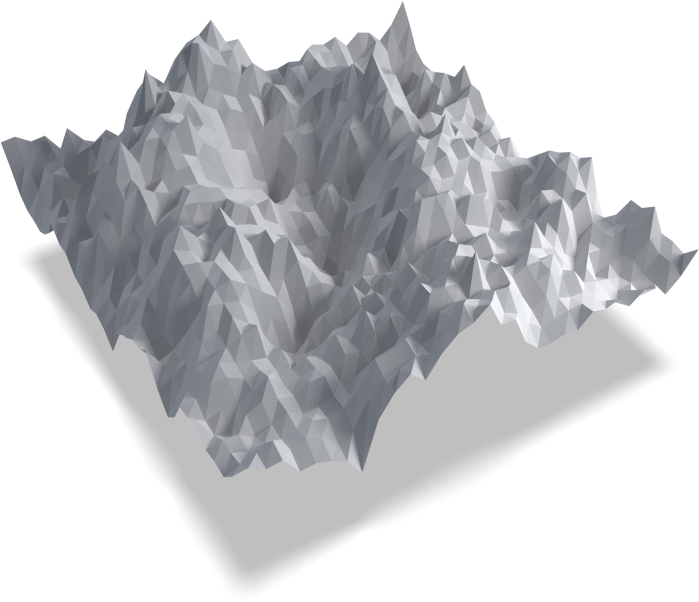
\includegraphics[width=0.5\textwidth]{./images/diamond_square/surface_blender/surface_composite01_cropped.png}%
    \caption{%
        A surface with resolution $33\times 33$ created using the midpoint displacement method called successive random additions.%
        \label{fig:diamond_square_surface}%
    }%
\end{figure}%
%
% \orangebox{
% {\bf Notes:}
% \begin{itemize}
%     \item Implementation (in Matlab/C++)?
%     \item periodic and non-periodic
%     \item Mention that DS can be used to increase resolution of any surface
%     \item Can increase resolution of generated surface, if we know the seed
% \end{itemize}
% 
% {\bf Stuff to define:}
% \begin{itemize}
%     \item Periodic/non-periodic
%     \item Lacunarity
% \end{itemize}
% }
            \subsection[Validation and examples]{Validation \hl{and examples?}}
\todoao{Write more about testing diamondsquare/SRA}%
\todobo{colormap plot from above of surface?}%
To test the method for generating random surfaces, and to check that the Hurst exponent of the surfaces correspond to the wanted exponent, we generate surfaces and measure the Hurst exponent using the detrending moving average method from \cref{sec:dma}. We have implemented both the midpoint displacement method and successive random additions for generating random surfaces, both for periodic and non-periodic surfaces. A plot of the measured Hurst exponent (using DMA) as function of the input Hurst exponent can be seen in \cref{fig:diamond_square_testing}.%
%
\begin{figure}[!htb]%
    \centering%
    {
        \newcommand{\f}{\footnotesize}%
        \newcommand{\x}{\text}%
        \newcommand{\hh}{{\f $H_\x{in}=H_\x{out}$}}%
        \includesvg[width=0.7\textwidth, svgpath=./images/diamond_square_Hurst/test_diamondSquare/]{fig06}%
    }
    %
    % ---- Footnotemark in caption, and footnotetext below ---- %
    \caption[%
        Plot of the Hurst exponent measured using detrending moving average (DMA), as function of the input Hurst exponent to the synthesizing method. The dashed grey line indicates a measured Hurst exponent of 0.75, the solid grey line a measured exponent exactly equal to the input exponent ($H_\text{in} = H_\text{out}$). The green lines are for surfaces created using periodic boundary conditions (PBC), the red lines using non-periodic boundaries, the dashed lines using successive random additions (SRA), and the solid lines using the regular midpoint displacement method (MDM). We used 100 samples for each point, and input Hurst exponents between 0 and 1.2 in steps of 0.1. We have plotted the standard deviation in each point for SRA with periodic boundary conditions, and the standard deviation is about the same for the other combinations. %
    ]{%
        Plot of the Hurst exponent measured using detrending moving average (DMA), as function of the input Hurst exponent to the synthesizing method. The dashed grey line indicates a measured Hurst exponent of 0.75, the solid grey line a measured exponent exactly equal to the input exponent ($H_\text{in} = H_\text{out}$). The green lines are for surfaces created using periodic boundary conditions (PBC), the red lines using non-periodic boundaries, the dashed lines using successive random additions (SRA), and the solid lines using the regular midpoint displacement method (MDM). We used 100 samples for each point, and input Hurst exponents between 0 and 1.2\protect\footnotemark\ in steps of 0.1. We have plotted the standard deviation in each point for SRA with periodic boundary conditions, and the standard deviation is about the same for the other combinations. %
        \hl{FINISH CAPTION} %
        \label{fig:diamond_square_testing}%
    }%
%     %
%     % ---- Footnote in caption, and separate lof caption ---- %
%     \caption[%
%         Plot of the Hurst exponent measured using detrending moving average (DMA), as function of the input Hurst exponent to the synthesizing method. The dashed grey line indicates a measured Hurst exponent of 0.75, the solid grey line a measured exponent exactly equal to the input exponent ($H_\text{in} = H_\text{out}$). The green lines are for surfaces created using periodic boundary conditions (PBC), the red lines using non-periodic boundaries, the dashed lines using successive random additions (SRA), and the solid lines using the regular midpoint displacement method (MDM). We used 100 samples for each point, and input Hurst exponents between 0 and 1.2 in steps of 0.1. We have plotted the standard deviation in each point for SRA with periodic boundary conditions, and the standard deviation is about the same for the other combinations.%
%     ]{%
%         Plot of the Hurst exponent measured using detrending moving average (DMA), as function of the input Hurst exponent to the synthesizing method. The dashed grey line indicates a measured Hurst exponent of 0.75, the solid grey line a measured exponent exactly equal to the input exponent ($H_\text{in} = H_\text{out}$). The green lines are for surfaces created using periodic boundary conditions (PBC), the red lines using non-periodic boundaries, the dashed lines using successive random additions (SRA), and the solid lines using the regular midpoint displacement method (MDM). We used 100 samples for each point, and input Hurst exponents between 0 and 1.2\protect\footnote{test} in steps of 0.1. We have plotted the standard deviation in each point for SRA with periodic boundary conditions, and the standard deviation is about the same for the other combinations. %
%         \hl{FINISH CAPTION} %
%         \label{fig:diamond_square_testing}%
%     }%
\end{figure}%
\footnotetext{In reality we can not have Hurst exponents greater than 1, but as we see, the midpoint displacement methods generally creates surfaces with a measured exponent ($H_\text{out}$) lower than the input exponent ($H_\text{in}$) for $H_\text{in}>0.5$, so to we use some samples of $H_\text{in}>1$.}%

From the plot in \cref{fig:diamond_square_testing} we see that surfaces with periodic boundaries generally get a lower measured $H$ than non-periodic surfaces, at least for the surfaces with $H>0.5$. We also see that the surfaces generated using the midpoint displacement method (MDM) have very similar Hurst exponents as the ones generated using successive random additions (SRA). We see that the Hurst exponent of all surfaces is generally lower than the input exponent for input $H>0.5$, and lower than the input exponent for input $H<0.5$. We should take note of this when generating surfaces for our experiments, and make sure to measure the actual exponent, since we see that the standard deviation is relatively high.%
\todobo{Something about why periodic surfaces have lower exponent?}
        \section{Generating fractures from surfaces\label{sec:generating_fractures}}
To generate a realistic fracture we use the method of successive random additions described in \cref{chap:generating_surfaces,subsec:SRA_implementation} to generate random surfaces with a known Hurst exponent. We then displace the surfaces in the $z$-direction, so one is above the other, and let the space between the surfaces be the void\footnote{Since we are using periodic systems, we could also have let the space outside the surfaces be the fracture and get the same result. But for easier visualization and understanding we use the volume between the surfaces.}.

In practice we make a fractured silica structure using the following procedure
\begin{itemize}
    \item Prepare a slab of amorphous SiO$_2$.
    \item Generate two surfaces.
    \item Rescale the $(x,y)$-positions of surfaces so they span the molecular system.
    \item Rescale the $z$-values of the surfaces so all points are inside the system.
    \item Remove all atoms between the upper and lower surface.
\end{itemize}

The biggest problem with this procedure is removing the atoms between two surfaces. But since all points in both surfaces lie on a regular grid in the $x$-$y$-plane, there is a simple way of dividing the volume between the surfaces into tetrahedra. And checking if a point is inside a tetrahedra is a geometrical exercize that can be solved programmatically. If the two surfaces are not intersecting, we can divide the volume between them into convex hexahedra spanned out by the points
% \begin{align*}
%     (x^1_{i}, y^1_{i}), (x^1_{i+1}, y^1_{i}), (x^1_{i}, y^1_{i+1}), (x^1_{i+1}, y^1_{i+1}), \\
%     (x^2_{i}, y^2_{i}), (x^2_{i+1}, y^2_{i}), (x^2_{i}, y^2_{i+1}), (x^2_{i+1}, y^2_{i+1}),
% \end{align*}
\begin{align*}
    z(i,j)&, & &z(i+1,j),& & &z(i,j+1)&, &\text{and}& & &z(i+1,j+1)& & &\text{for} & &i,j \in [0,N)
\end{align*}
in the two surfaces (four points in each surface). We then divide each convex hexahedra into five tetraheda, as illustrated in \cref{fig:hex_to_tetra}, giving a total of $5(N-1)^2$ tetrahedra spanning the total volume between the two surfaces.
%
% We do this by utilizing the fact that the points in each heighmap lie on a regular grid in the $x$-$y$-plane. This means that we can divide the volume into tetrahedra, . If the two heightmaps are not intersecting, we see that we can divide the volume between them into convex hexahedra, one for each set of points
% ($x_{i}, y_{i}$), ($x_{i}, y_{i+1}$), ($x_{i+1}, y_{i}$), and ($x_{i+1}, y_{i+1}$) 
% % $(x_i, y_i)$  $(x_i, y_{i+1})$ $(x_{i+1}, y_i)$ $(x_{i+1}, y_{i+1})$
% in the $x$-$y$-grid. Each of these hexahedra can then be divided into five tetrahedra, as illustrated in \cref{fig:hex_to_tetra}.
%
% \begin{figure}[htpb]%
%     \centering%
%     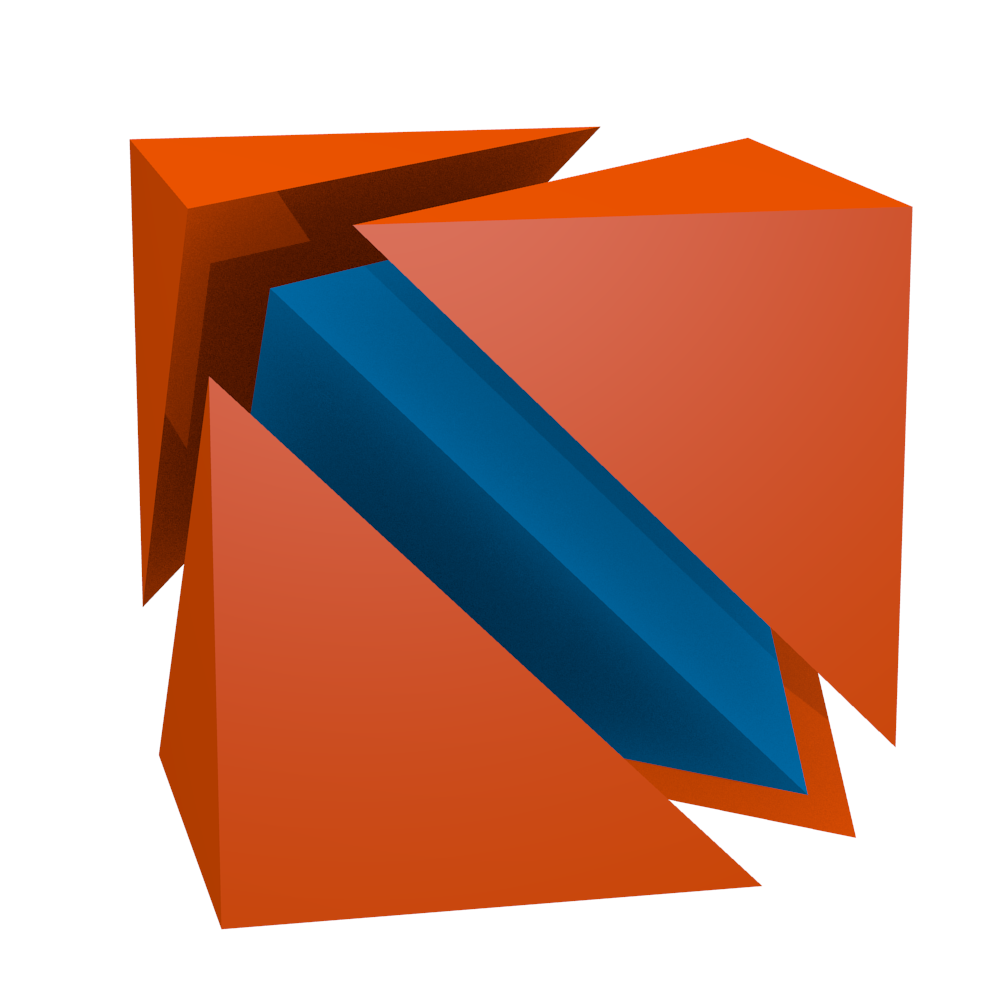
\includegraphics[width=0.4\textwidth]{images/fracture/hexahedron_to_tetrahedra.png}%
%     \caption{%
%         Illustration of how to divide a hexahedron into five tetraheda.%
%         \label{fig:hex_to_tetra}%
%     }%
% \end{figure}%
% %
% \begin{figure}[htpb]%
%     \centering%
%     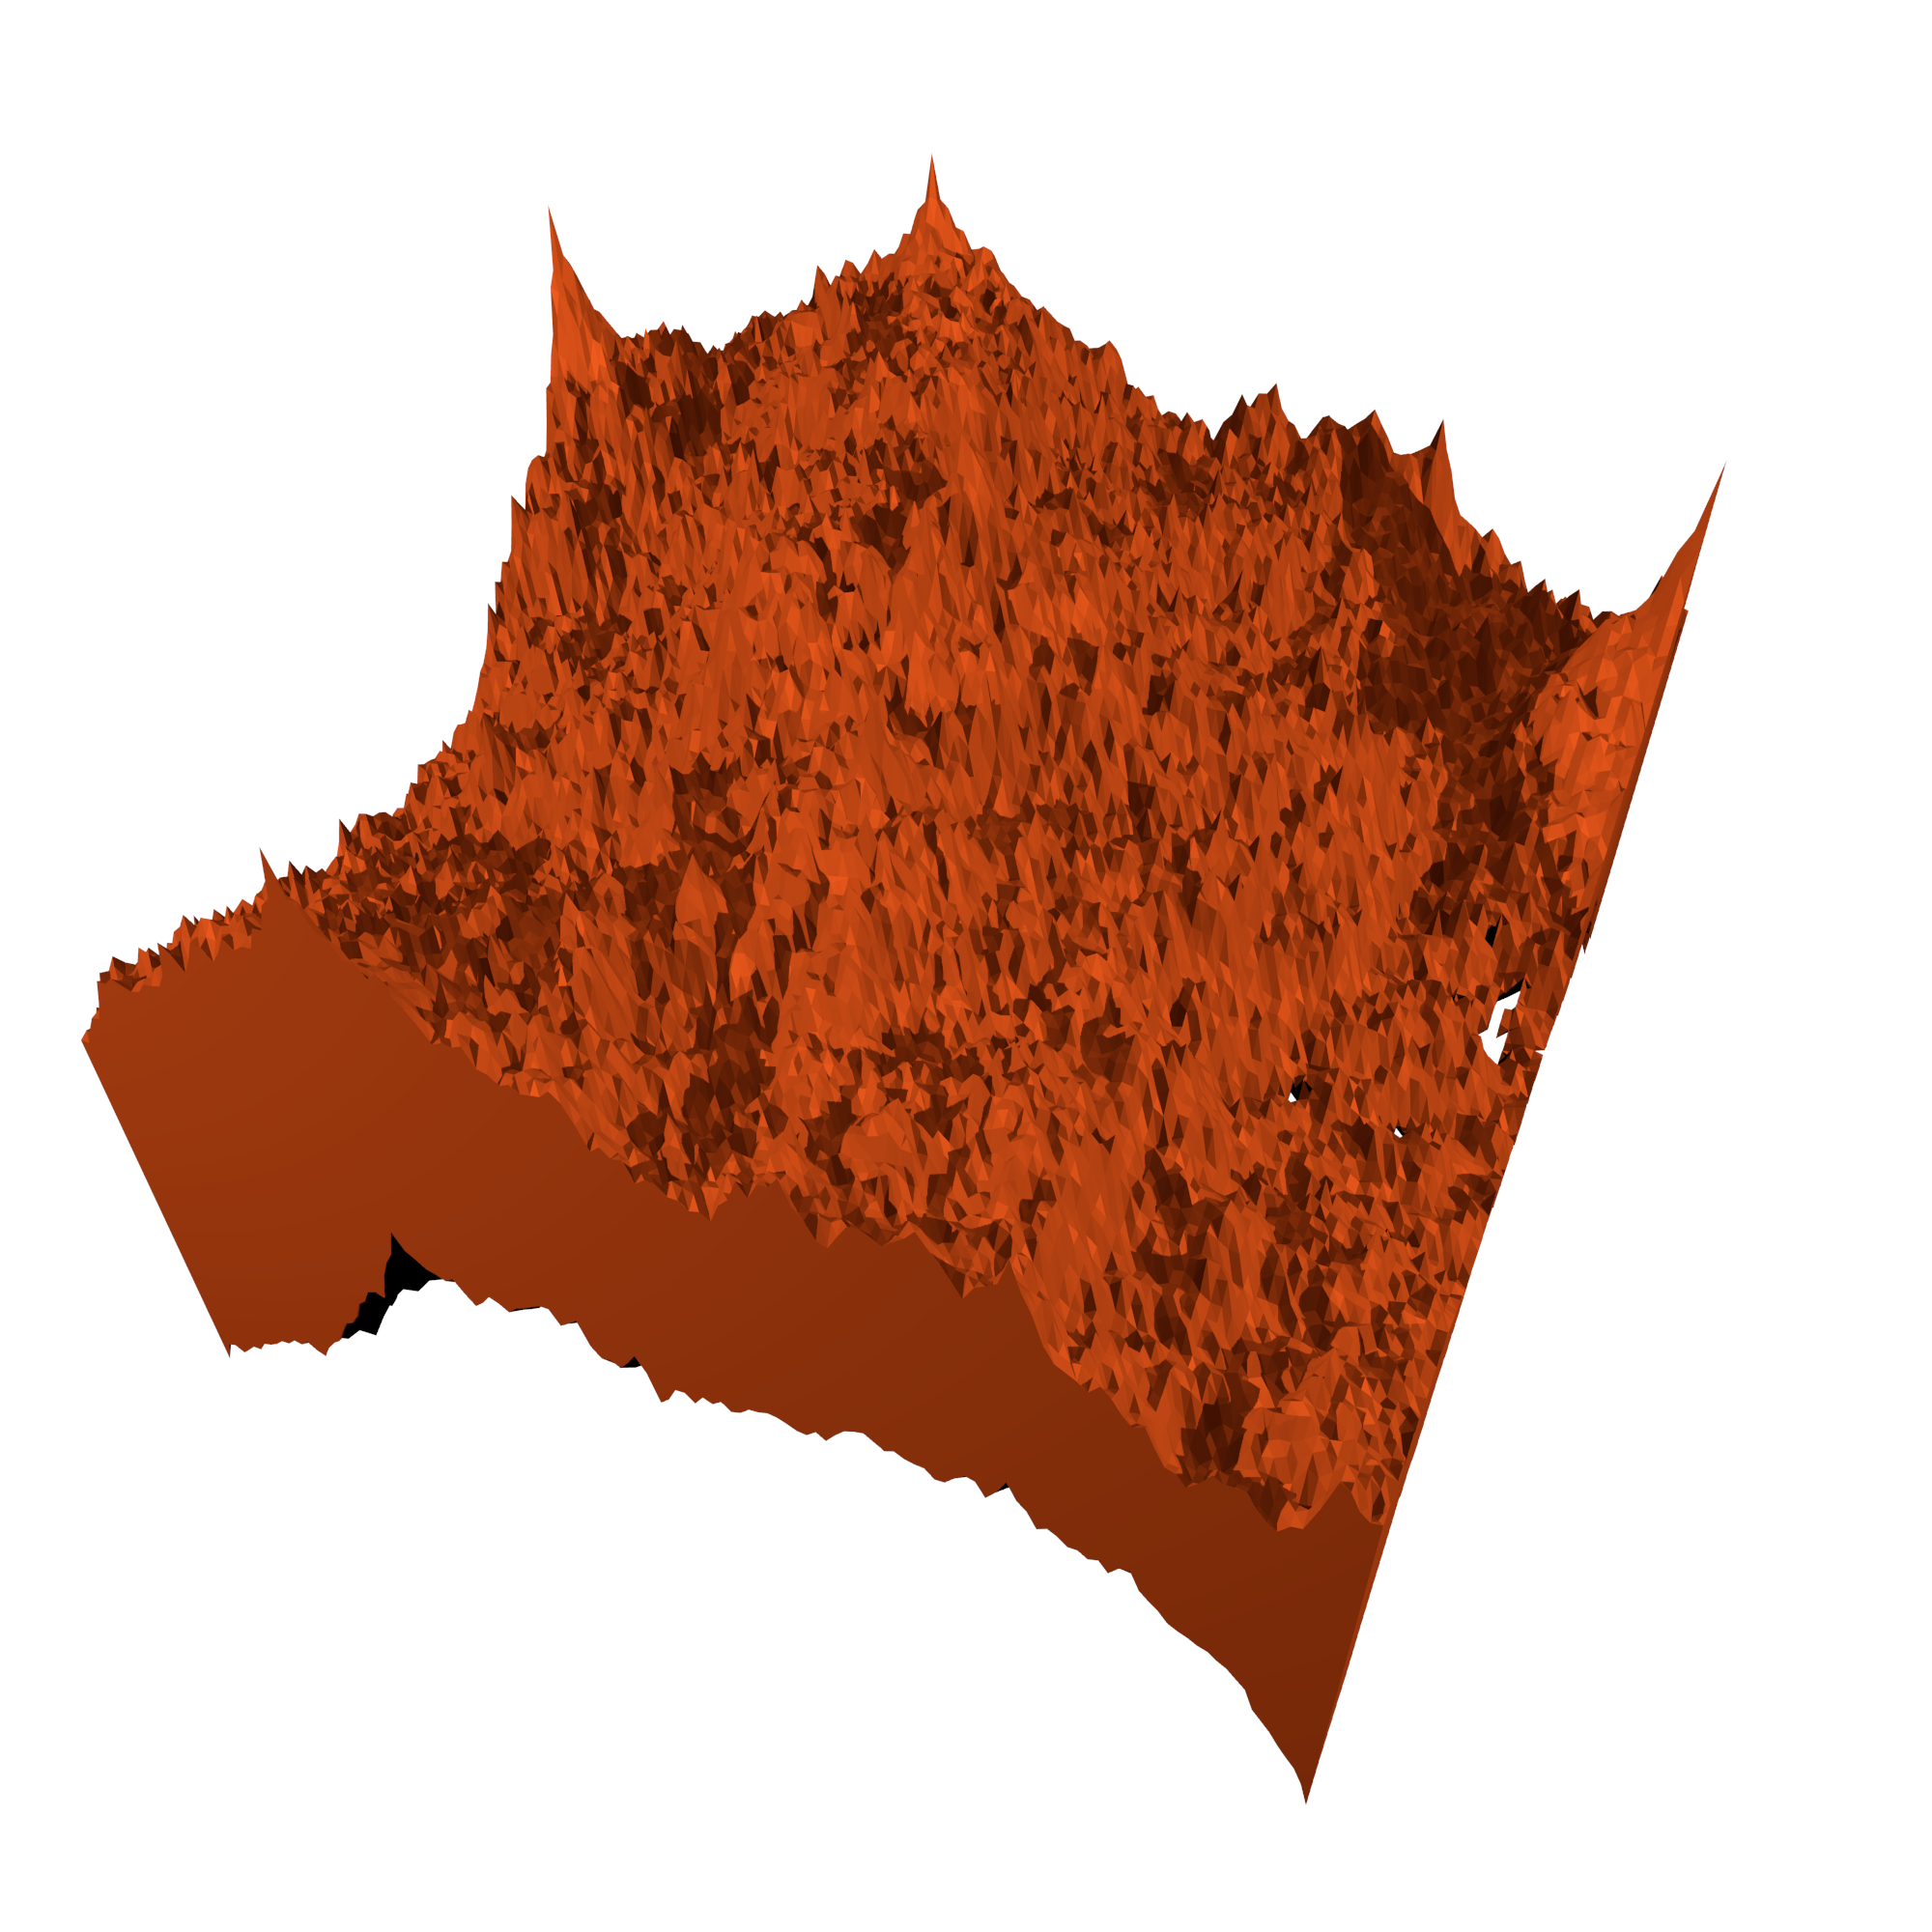
\includegraphics[width=0.6\textwidth]{images/fracture/fracture.png}%
%     \caption{%
%         A model of a fracture.%
%         \label{fig:fracture_model}%
%     }%
% \end{figure}%
%
\begin{figure}[htpb]%
    \centering%
    \setlength{\myfigwidth}{0.4\textwidth}%
%     \setlength{\mycaptionwidth}{0.3\textwidth}%
    \begin{subfigure}[b]{\myfigwidth}%
        \centering% % Need to center to get image centered over caption
        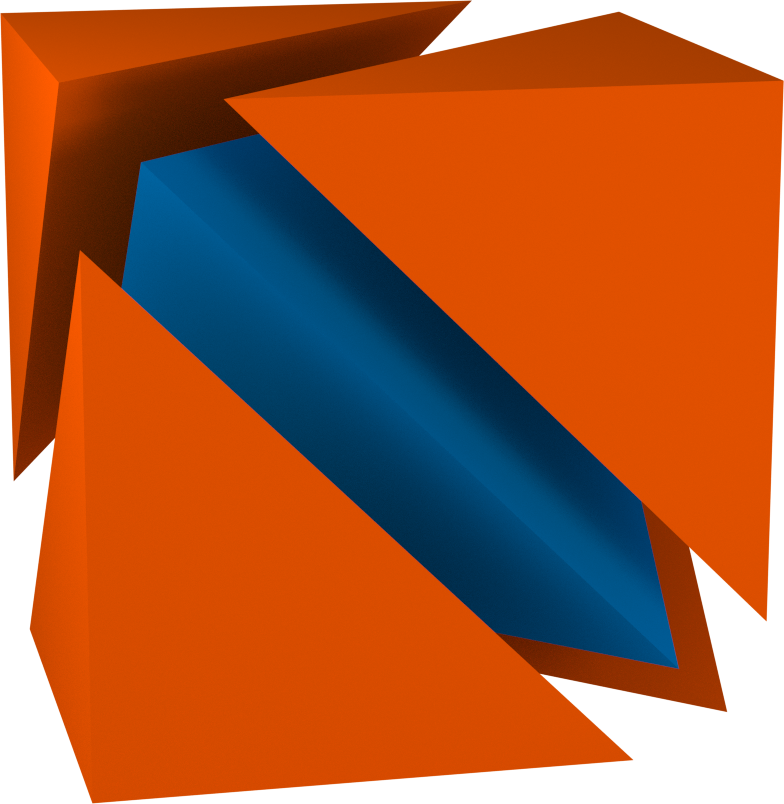
\includegraphics[width=0.6\textwidth]{images/fracture/hexahedron_to_tetrahedra01_cycles_n200_cropped.png}%
        \caption{Illustration of how to divide a convex hexahedron into five tetraheda.}%
        \label{fig:hex_to_tetra}%
    \end{subfigure}%
    \hspace{0.1\textwidth}%
    \begin{subfigure}[b]{\myfigwidth}%
        \centering%
        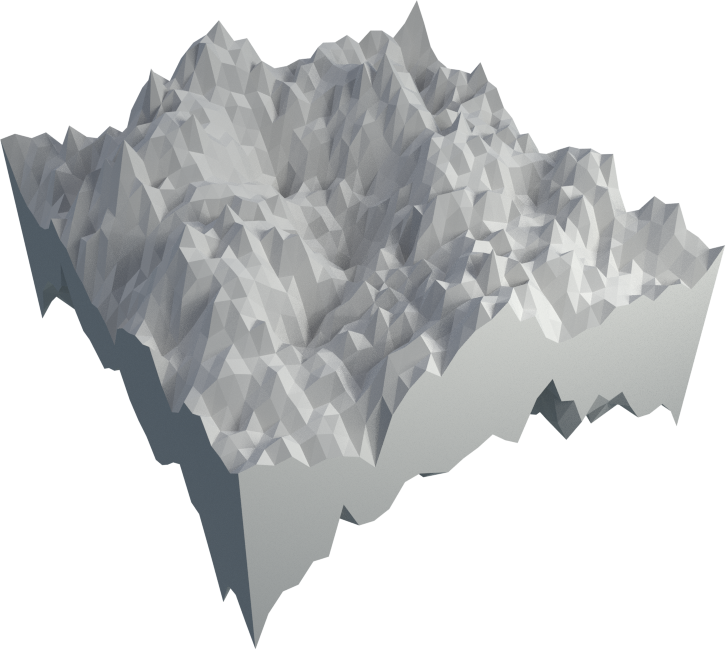
\includegraphics[width=\textwidth]{images/fracture/fracture05_n200_cropped.png}%
%         \includegraphics[width=\textwidth]{images/fracture/large_fracture04_300dpi_w20cm}%
        \caption{A random fracture made from two periodic surfaces.}%
        \label{fig:fracture_model}%
    \end{subfigure}%
\end{figure}%
            \subsection{Finding a point inside a tetrahedron}
A tetrahedron consists of four points $\bvec a$, $\bvec b$, $\bvec c$, and $\bvec d$, and four faces spanned by the four possible combinations of the four points. For a face spanned by the points $\bvec a$, $\bvec b$, and $\bvec c$ we can find if a point $\bvec P$ is on the same side of the face as the point $\bvec d$ (the point not used to construct the face) by doing some geometry. We first find the normal vector to the surface $\bvec n$ by the cross product 
\begin{align*}
    \bvec n = (\bvec a-\bvec c)(\bvec b-\bvec c).
\end{align*}
We know that the sign of the dot product between this normal vector and another vector going from the plane to a point will give us information about which side of the plane the point is. This means that if two points $\bvec p_1$ and $\bvec p_2$ are on the side of the plane, the dot product between the normal vector and the two vectors
\begin{align*}
    (\bvec p_i - \bvec k),
\end{align*}
where $\bvec k$ is any point in the plane, should have the same sign. So we find the sign of dot products
\begin{align*}
    &\text{sgn}\big(\bvec n\cdot(\bvec P - \bvec k)\big), \\
    &\text{sgn}\big(\bvec n\cdot(\bvec d - \bvec k)\big),
\end{align*}
and if the sign of these dot products is the same, we know that the point $\bvec P$ is on the same side of the face as the point $\bvec d$. We now see that if we do this for all four faces of the tetrahedra, we know that the point $\bvec P$ is inside the tetrahedra if the signs of \emph{all} pairs of dot products are equal.

To implement this for checking which atoms are between two surfaces (with the volume between the surfaces divided into tetrahedra), we express it as a matrix equation. This reduces the calculation of wether a point is inside a tetrahedron to comparing the signs of five matrix determinants.

% Calculating wether a point is inside a tetrahedron can be reduced to comparing the sign of five different matrix determinants. If we have a point $P = (x,y,z)$ and the four vertices of the tetrahedron are $(x_i, y_i, z_i)$ for $i\in \{1,2,3,4\}$, we can find if the point is inside the tetrahedron by checking if the the following five matrix determinants have the same sign
% \begin{align*}
%     &\begin{vmatrix}
%         x_1 & y_1 & z_1 & 1 \\
%         x_2 & y_2 & z_2 & 1 \\
%         x_3 & y_3 & z_3 & 1 \\
%         x_4 & y_4 & z_4 & 1
%     \end{vmatrix},&
%     &\begin{vmatrix}
%         x & y & z & 1 \\
%         x_2 & y_2 & z_2 & 1 \\
%         x_3 & y_3 & z_3 & 1 \\
%         x_4 & y_4 & z_4 & 1
%     \end{vmatrix},&
%     &\begin{vmatrix}
%         x_1 & y_1 & z_1 & 1 \\
%         x & y & z & 1 \\
%         x_3 & y_3 & z_3 & 1 \\
%         x_4 & y_4 & z_4 & 1
%     \end{vmatrix},&
%     \\
% %     \vspace{5mm}
%     \\
%     &\begin{vmatrix}
%         x_1 & y_1 & z_1 & 1 \\
%         x_2 & y_2 & z_2 & 1 \\
%         x & y & z & 1 \\
%         x_4 & y_4 & z_4 & 1
%     \end{vmatrix},&
%     &\begin{vmatrix}
%         x_1 & y_1 & z_1 & 1 \\
%         x_2 & y_2 & z_2 & 1 \\
%         x_3 & y_3 & z_3 & 1 \\
%         x & y & z & 1
%     \end{vmatrix}.&
% \end{align*}


\part{Simulations}
    \chapter*{Introduction}%
\addcontentsline{toc}{chapter}{Introduction}%
In this chapter we will present the procedure we have used when doing simulations, the systems we have studied, and the the results we have found. 

We start with a description of what steps we have used to generate a realistic nanoporous silica, with water in the pores. We describe how we create a random fracture in a slab of silica, and the method we have developed for passivating the dangling ends after we cut out the fracture. We also describe a method for injecting water into the fracture.

After this we present the different measurements we have done during the simulations, how the measurements are done, and why we do them. We then describe the different systems we have generated, the characteristics of these systems, both in form of tables, and using renderings of visualizations of the systems.

Finally the results from all our simulations and measurements are presented and discussed. \todoao{Some more intro to results?}
    \chapter{Simulation procedure}
% \todob{In experiments: mention smaug}
\todobo{In experiments: mention phase transitions of silica and water? Water has same phase even if we have high pressure/density}%
\todobo{Steepest descent procedure?}%
%
When doing simulations using molecular dynamics we use a procedure akin that used by actual experiments. Since the duration of the simulations we are realistically able to simulate on are of the order of tens of nanoseconds, we have to be smart when initializing the system, to avoid having to simulate for a long time to get to the state we want to study. This means that we should start out with the system in a state as close to the one we want to study as possible. The problem with this when simulating silica is that the silica structure formed when rapidly cooling molten silica does not have any long-range ordering. Silica in the glass form has an amorph structure, which does not have any long-range ordering, but has short-range ordering well beyond the Si-O bond length. This structure is hard to set up with an algorithm.
        \section{Initialization\label{sec:experimental_procedure}}
To generate silica in the glass form we first create a perfect silica crystal in the crystalline form $\upbeta$-cristobalite, the unit cell of which can be seen in figure \cref{fig:beta_cristobalite-unit_cell}, and a larger crystal in \cref{fig:cristobalite_crystal}. This crystalline form consists of corner-bonded SiO$_4$-tetrahedra, and in the perfect crystallic form all silicon atoms are bound to four oxygen atoms, and all oxygen atoms to two silicon atoms. 

We give the atoms a random uniformly distributed velocities with mean $\mu = 0$ and standard deviation $\sigma \propto \sqrt{T}$, where $T$ is the wanted temperature.%
\begin{figure}[htb]%
    \centering%
    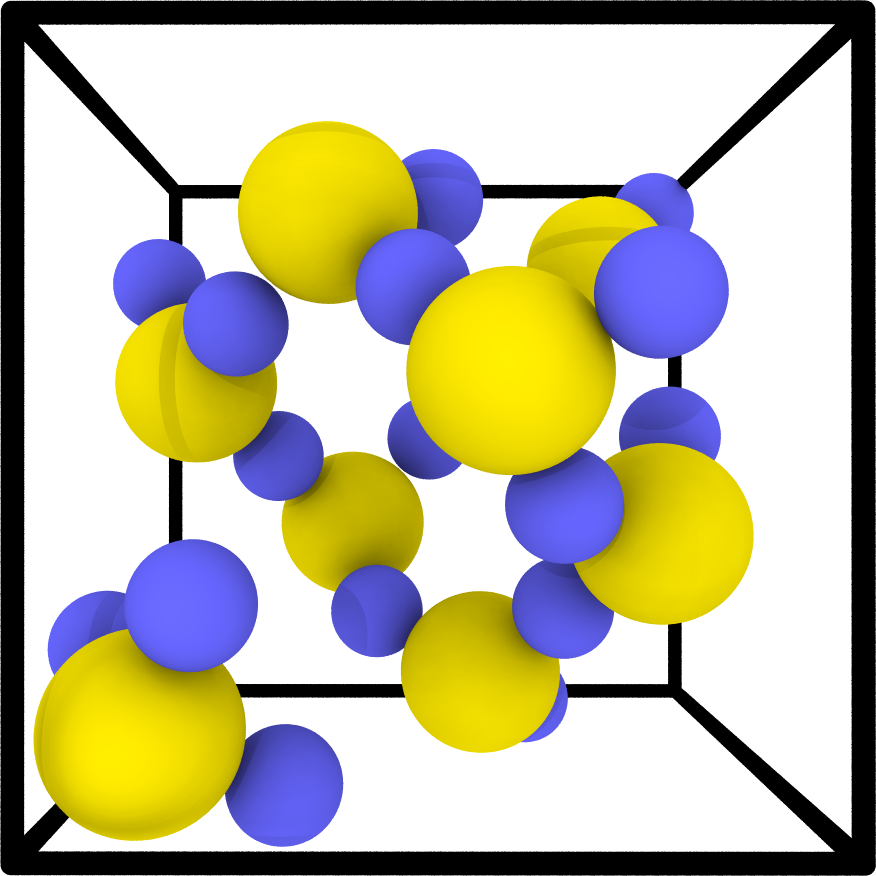
\includegraphics[width=0.4\textwidth]{images/beta_cristobalite/unit_cell05_cropped.png}%
    \caption{%
        $\upbeta$-cristobalite unit cell, with 8 silicon atoms and 16 oxygen atoms.%
        \label{fig:beta_cristobalite-unit_cell}%
    }%
\end{figure}%

We then heat the system to 4500 K in steps of 700 K to melt the silica crystal. Since we are mainly interested in controlling the temperature at this stage, the Berendsen thermostat is used for these temperature changes. We alternate between using a thermostat to adjust the temperature, and simulating with the thermostat off, to let the system thermalize and react to the temperature change after applying the thermostat. The number of timesteps we used for the thermostat period is around 2 500, and for the thermalization period around 10 000. We then cool the system by doing the previous procedure in reverse. See \cref{fig:plot_heat_melt_sio2} for a plot of the temperature as function of time while we melt and cool down the system, and \cref{fig:initialization_step00} for a visualization of a perfect crystal of $\upbeta$-cristobalite, and \cref{fig:initialization_step02} for amorphous, solid silica.%
%
\begin{figure}[htpb]%
    \centering%
    \includesvg[width=0.6\textwidth, svgpath = ./images/energy_plots/]{system00_temperature_melt_cool}%
    \caption{%
        Plot of the temperature (in kilo-Kelvin) as function of timesteps when melting and cooling down a silica system, using the Berendsen thermostat. We use timesteps of 0.050 picoseconds, and use 2 500 timesteps with the thermostat turned on, and then 10 000 timesteps to let the system thermalize (with the thermostat off), for each step in temperature. %
        \label{fig:plot_heat_melt_sio2}%
    }%
\end{figure}%
%
% \todob{Reference figures below, say something about energy conservation \cref{fig:plot_heat_melt_sio2,fig:plot_energy_conservation}}
% \todoco{Silica phase diagram? for melting, phases etc. - Not needed according to Malthe}

The initialization procedure is visualized in \cref{fig:initialization_steps}, and can be summed up as follows
\begin{itemize}
    \item Generate a perfect crystal of $\beta$-cristobalite of the wanted size (\cref{fig:initialization_step00}).
    \item Heat the system to well above the melting point of silica (we usually use 4 500 Kelvin, using a thermostat (Berendsen) (\cref{fig:initialization_step01}).
    \item Cool down the system to well below the glass-transition temperature (we use 300 Kelvin), using a thermostat (Berendsen) (\cref{fig:initialization_step02}).
    \item Cut out the fracture (\cref{fig:initialization_step03}).
    \item Passivate the dangling ends and apply steepest descent to let the passivation atoms find their optimal positions (\cref{fig:initialization_step04}).
    \item Fill the pore with water, and thermalize the system at 300 K (\cref{fig:initialization_step05}).
\end{itemize}
%
\begin{figure}[htpb]%
%     \captionsetup{width=1.4\textwidth}%
    \setlength{\myfigwidth}{0.35\textwidth}%
    %
    \setlength{\myhfillwidth}{1.5cm}%
    \centering%
    \begin{subfigure}[t]{\myfigwidth}
        \captionsetup{width=1.1\textwidth}%
        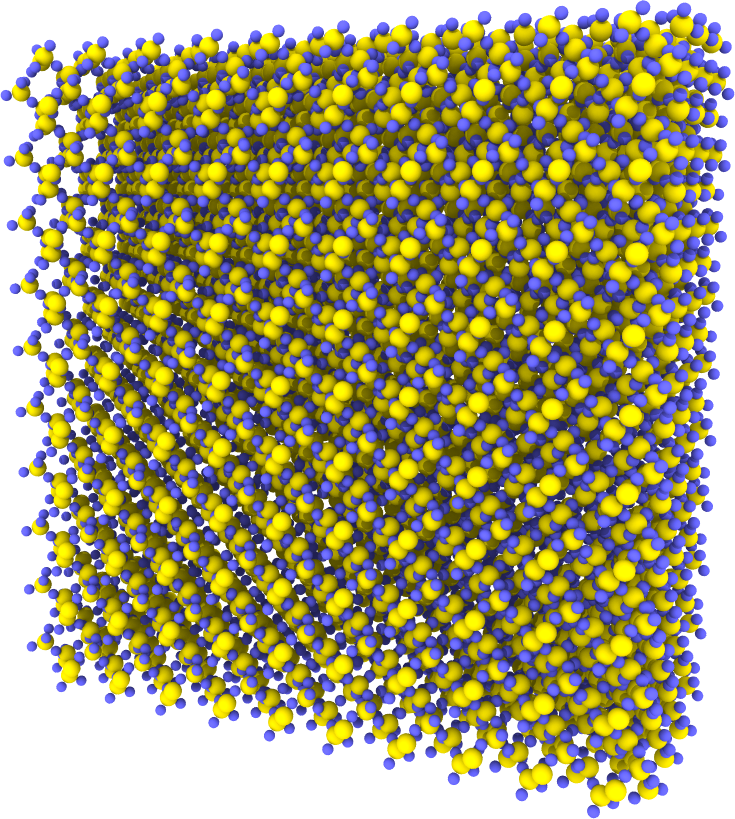
\includegraphics[width=\textwidth]{images/experimental_procedure/00_10}%
        \caption{%
            Perfect $\upbeta$-cristobalite crystal.%
            \label{fig:initialization_step00}%
            \label{fig:cristobalite_crystal}%
        }%
        \hspace{8pt}
    \end{subfigure}%
    \hspace{\myhfillwidth}%
    \begin{subfigure}[t]{\myfigwidth}%
        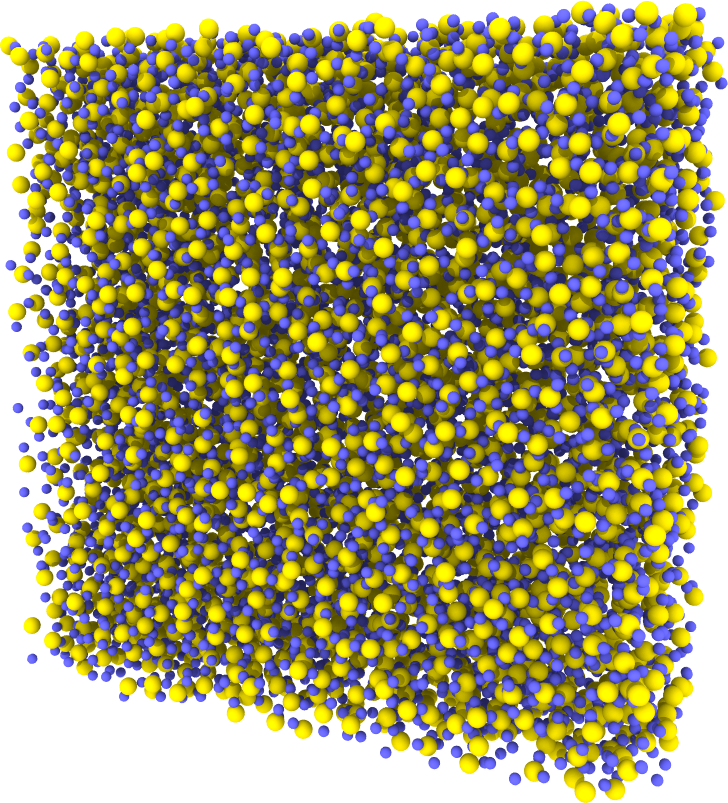
\includegraphics[width=\textwidth]{images/experimental_procedure/01_10}%
        \caption{%
            Silica heated to 4500 K.%
            \label{fig:initialization_step01}%
        }%
        \hspace{8pt}
    \end{subfigure}%
    \\%
    \begin{subfigure}[t]{\myfigwidth}%
        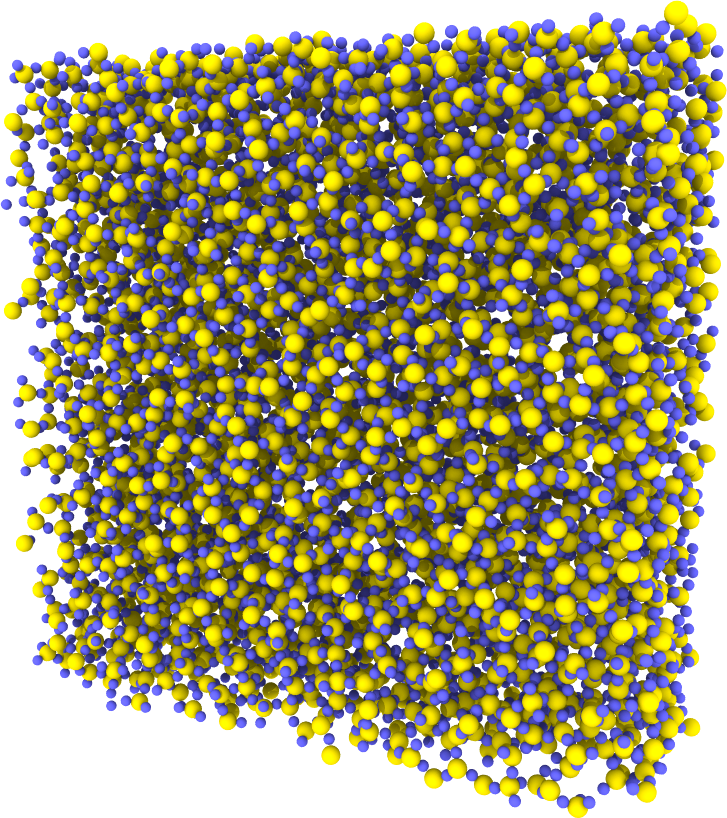
\includegraphics[width=\textwidth]{images/experimental_procedure/02_10}%
        \caption{%
            Silica cooled to 300 K.%
            \label{fig:initialization_step02}%
        }%
    \end{subfigure}%
    \hspace{\myhfillwidth}%
    \begin{subfigure}[t]{\myfigwidth}%
        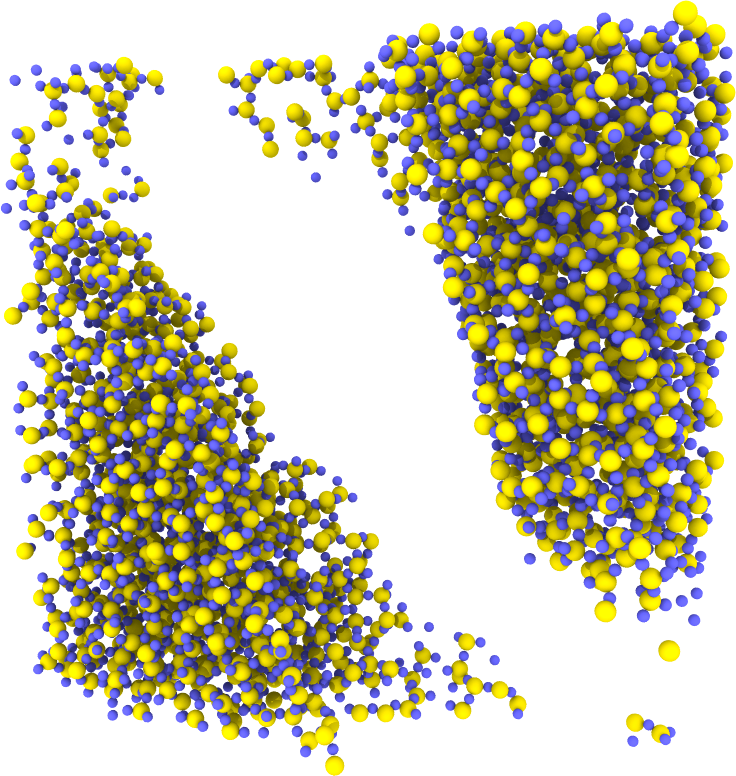
\includegraphics[width=\textwidth]{images/experimental_procedure/03_10}%
        \caption{%
            Fracture cut out.%
            \label{fig:initialization_step03}%
        }%
        \hspace{8pt}
    \end{subfigure}%
    \\%
    \begin{subfigure}[t]{\myfigwidth}%
        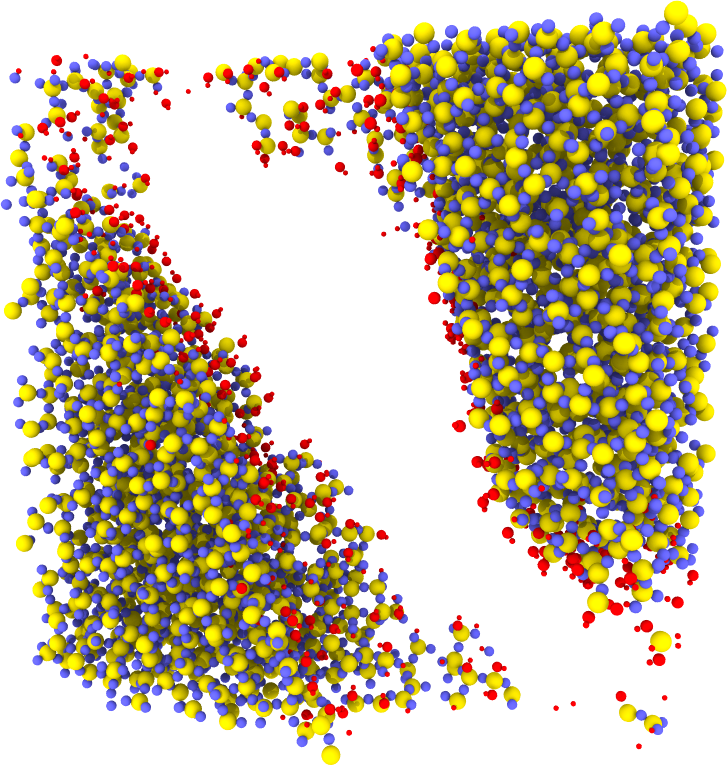
\includegraphics[width=\textwidth]{images/experimental_procedure/04_10}%
        \caption{%
            Dangling ends passivated.%
            \label{fig:initialization_step04}%
        }%
        \hspace{8pt}
    \end{subfigure}%
    \hspace{\myhfillwidth}%
    \begin{subfigure}[t]{\myfigwidth}%
        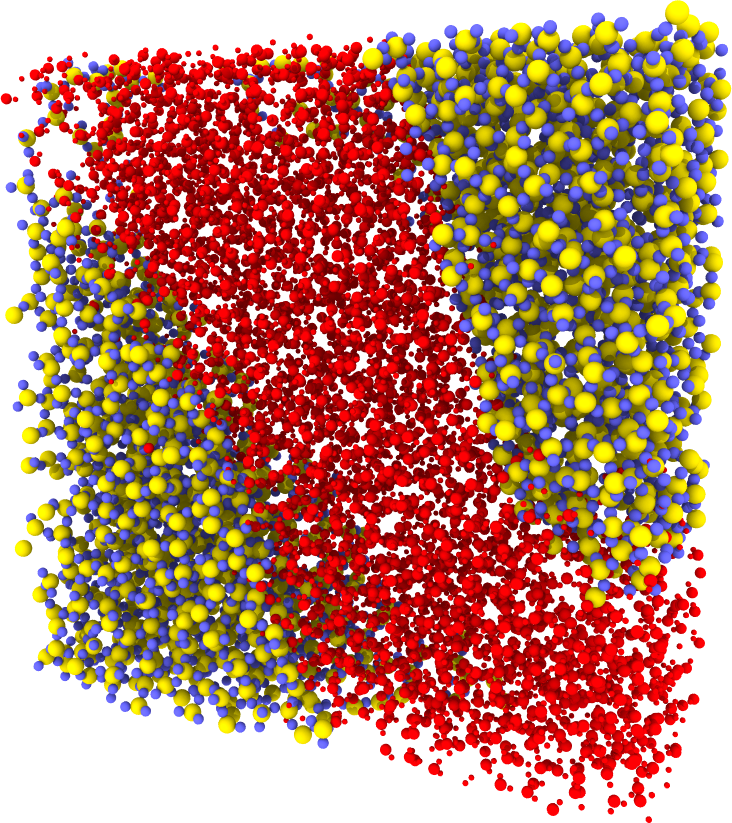
\includegraphics[width=\textwidth]{images/experimental_procedure/05_10}%
        \caption{%
            Pore filled with water.%
            \label{fig:initialization_step05}%
        }%
        \hspace{8pt}
    \end{subfigure}%
    \captionsetup{width=\textwidth}%
    \caption{%
        Visualizations of the different stages of initialization of a fracture in silica filled with water. We show a $75\times 75\times 25$ \AA\ slice of a much larger system $(172 \text{ \AA})^3$. The silicon atoms are yellow, the silica-oxygen blue, and hydrogen and water-oxygen red. %
        \label{fig:initialization_steps}%
    }%
\end{figure}%

We now have a thermalized and (hopefully) realistic silica crystal at near room temperature. From this crystal we cut out the fracture, passivate using one of the passivation methods, fill the fracture with water molecules, and apply a simple steepest descent procedure to let the inserted atoms find their equilibrium positions. After filling the fracture with water we need to thermalize the system again, since the energy (and thereby the temperature) changes when we remove and insert atoms.
        \section{Passivation}
In most silicates the silicon atoms have tetrahedral coordination, with four oxygen atoms surronding each silicon atom. When we remove silica- and oxygen-atoms to create a fracture, we do not take this into consideration. This means that we get dangling unsaturated bonds in the system, located near the surface of the pore. To rectify this we use a method called passivation, where we saturate and passivate the dangling bonds by inserting new atoms. 

\subsection{Water chemistry}
Since we are going to inject water into the pore later on, we want to use the constituents of water to passivate the system. We know that water autodissociates into H$^{+}$ and OH$^{-}$ via the following reaction
\begin{align*}
    \text{H}_2\text{O} \rightleftharpoons \text{H}^{+} + \text{OH}^{-},
\end{align*}
meaning that hydrogen (H) and hydroxide (OH) will be freely available in the system after filling the pore with water. On this background we choose to passivate the system using hydrogen and hydroxide. To avoid getting an acidic or alkaline system after the passivation procedure we should make sure to use equal parts hydrogen and hydroxide when passivating.

\subsection{Passivating using hydrogen and hydroxide}
After thermalizing our silica system we end up with a system consisting almost exclusively of SiO$_2$ tetrahedra. These tetrahedra are each formed by four oxygen atoms, one in each corner, and a silicon atom in the center. Each of these tetrahedra are then bonded to four other tetrahedra, by sharing the oxygen atoms in the corners. This way each oxygen atom is bonded to two silicon atoms, and each silicon atom to four oxygen atoms, giving an average chemical formula of SiO$_2$. 

Since we do not take chemical bonds into consideration when removing atoms to create a fracture, we end up with some incomplete tetrahedra, with some silicon atoms bonded to less than four oxygen atoms, and some oxygen atoms bonded to less than two silicon atoms. See \cref{fig:passivation} for an illustration of three different incomplete tetrahedra. This creates what we call dangling ends or unsaturated bonds, which we want to passivate.

% When inserting hydrogen and hydroxide we want to insert them in positions that are close to their equilibrium positions, so we do not have to do a lot of simulating to get a stabilized system after passivating. It is possible to calculate the optimal positions based on the potential and the positions of the existing atoms, but this is a complicated computation, that we can avoid, by instead realizing that the optimal positions for the oxygen atoms we insert will most likely \hl{(source?)} be close to the positions that complete the SiO$_2$ tetrahedra. These positions can be calculated, using simple geometry, from the positions of the oxygen atoms each silicon atom is bonded to.

To passivate the silicon atoms that are bonded to less than four oxygen atoms, we see that we need to complete the incomplete SiO$_4$ tetrahedra that have been created in the system. But if we only insert oxygen atoms in the positions of the missing oxygen atoms, we end up with new dangling ends, since the inserted oxygen atoms will only be bonded to one silicon atom. But, as we just saw, we will have hydroxide (OH) groups available in the system after filling the fracture with water. So instead of inserting oxygen atoms and creating new unsaturated bonds, we insert hydroxide groups and create saturated Si-O-H bonds. We put the hydrogen atom so that the Si-O-H angle is close to the angle in water molecules, 107.5 degrees. %\hl{The hydrogen atoms moves very rapidly compared to the rest of the species in the system, so they will quicly find the equilibrium position, meaning that the exact position of the hydrogen atoms is not that important.}

To passivate the oxygen atoms that are bonded to only one silicon atom, we can use the hydrogen atoms that are avilable after filling the fracture with water, turning unsaturated SiO-groups into the same saturated Si-O-H-groups as before. We here too insert the hydrogen atoms with the Si-O-H angle close to 107.5 degrees.

In total we use the following procedure to passivate a system after creating a fracture:
\begin{itemize}
    \item Remove all silicon and oxygen atoms that are not bonded to any atoms, since they are essentially not part of the silica matrix.
    \item Add one hydrogen atom to all oxygen atoms bonded to only one silicon atom. The hydrogen atoms are inserted approximately $0.95\text{ \AA}$ from the oxygen atoms, with the hydrogen atom pointing away from the silicon atom, and with the Si-O-H angle close to 107.5 degrees.
    \item Add ($4-n$) hydroxide groups to silicon atoms bonded to $(1\leq n<4)$ oxygen atoms. We assume that the most stable position for the oxygen in the hydroxide groups are close to the tetrahedral positions of the missing oxygen atoms, and insert the hydroxide groups in these positions. %
    %See \cref{fig:pass_tet01,fig:pass_tet02,fig:pass_tet03} for the three different cases. 
    The hydroxide groups are inserted approximately $1.65\text{ \AA}$ from the silicon atoms, measured from the position of the silicon atom to the oxygen atom in the hydroxide groups, with the hydrogen atom pointing away from the silicon atom, and with the Si-O-H angle close to 107.5 degrees.
\end{itemize}
The lengths used are approximate experimental lengths found in naturally occuring silanols and water (see \cite{lickiss1995synthesis} for the Si-O length in silanol, and \cite{csaszar2005equilibrium} for the O-H length in water). This procedure turns all dangling ends into stable, passive silanol groups.
%
\begin{figure}[htpb]%
    \centering%
    \setlength{\myfigwidth}{0.17\textwidth}
    \begin{subfigure}[c]{0.8\myfigwidth}%
        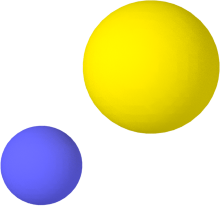
\includegraphics[width=\textwidth]{images/passivation/tetrahedra01_01.png}%
        \caption{}%
%         \caption{Illustration of how to divide a convex hexahedron into five tetraheda.}%
        \label{fig:pass_tet01}%
    \end{subfigure}%
    \hspace{1cm}%
    \begin{subfigure}[c]{\myfigwidth}%
        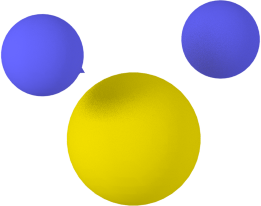
\includegraphics[width=\textwidth]{images/passivation/tetrahedra02_01.png}%
        \caption{}%
%         \caption{A random fracture made from two periodic heightmaps.}%
        \label{fig:pass_tet02}%
    \end{subfigure}%
    \hspace{1cm}%
    \begin{subfigure}[c]{1.1\myfigwidth}%
        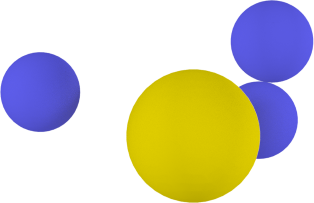
\includegraphics[width=\textwidth]{images/passivation/tetrahedra03_01.png}%
        \caption{}%
%         \caption{A random fracture made from two periodic heightmaps.}%
        \label{fig:pass_tet03}%
    \end{subfigure}%
    \hspace{1cm}%
    \begin{subfigure}[c]{1.1\myfigwidth}%
        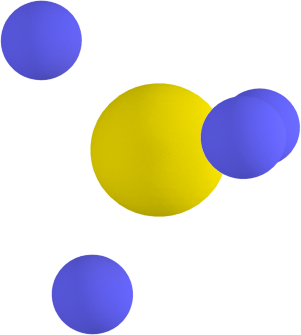
\includegraphics[width=\textwidth]{images/passivation/tetrahedra04_01.png}%
        \caption{}%
%         \caption{A random fracture made from two periodic heightmaps.}%
%         \label{fig:fracture_model}\caption{}%
    \end{subfigure}%
    \caption{%
        Illustration of four different incomplete silica tetrahedra, with respectively one, two, three and no missing oxygen atoms (\textbf{(d)} is a complete silica tetrahedra).%
    }%
    \label{fig:passivation}%
\end{figure}%

\subsection{Counting number of bonds}
Since we do not have actual bonds in molecular dynamics simulations, we do not know which atoms are bonded to which. So to find the number of bonded atoms for each silicon and oxygen atom, we create what we call \emph{neigbor lists}. These neighbor lists are a list of atoms within a chosen radius for each atom. To create these lists we use the procedure detailed in \cref{sec:neighbor_lists}. Since we only have silicon and oxygen atoms in our system, we only need to specify a maximum the Si-O-distance to find which atoms are bonded. If we choose this distance properly, we should be able find a good approximation to how many atoms each atom is bonded to.%
\todobo{Something about g(r) for deciding Si-O bond length, or potential parameters?}

% \orangebox{
% \begin{itemize}
%     \item What Si-O distance did we use to find bonds? Why? 
%     \item g(r) for Si-O?
%     \item Implementation?
%     \item Visualization of results?
%     \item What to do about atoms that can not be passivated (because we have to insert passively)?
% \end{itemize}
% }

% \subsection{Implementation}
% To implement the passivation procedure detailed above we see that we can make an  

% \begin{itemize}
%     \item Tetrahedra
%     \item Neighbor lists -- see base\_code/passivate\_using\_tetrahedra/passivator.cpp near line 700
%     \begin{itemize}
%         \item Create list of atoms in each voxel
%         \item Create neighbor lists for each atom by looping through neighbor voxels for each atoms
%     \end{itemize}
%     \item Count number of neighbors of different types -- find number of missing neighbors, Si - 4 Oxygen, Oxygen 2 Si
%     \item Insert OH on Si with missing O neighbors, insert H on Oxygen with missing Si neighbors
%     \begin{itemize}
%         \item Insert O/H at good angles
%     \end{itemize}
%     \item Improvement: find the atoms near surface using voxels, only passivate those atoms
% \end{itemize}

\subsection{Only passivating surface atoms}
When implementing the passivation method detailed above, we soon ran into problems with silica and oxygen atoms that were bonded to too few atoms according to our rules above, while counting the number of bonds using a fixed radius. Some improvements were made by fine-tuning the radius used for each atom type, but we still often ended up passivating atoms that were inside the silica matrix, where we should not have any dangling bonds. To avoid this we came up with a method to only passivate the atoms at or near the surface of the fracture.

To do this we yet again use the voxelation method from \ref{sec:voxelation}, but this time we use a voxel size of around $6\text{ \AA}$. We then mark all voxels with atoms in them as occupied. We now see that if we find all \emph{occupied} voxels with at least one \emph{unoccupied} neighbor voxel (using 26-neighbor connectivity), we should have a list of the voxels that make up the surface of the fracture, and these voxels then contain all atoms at or near the surface of the fracture. We then use this list of atoms as input to the passivation program, and only passivate atoms in that list. See \cref{fig:find_surface_atoms} for an illustration of the method that finds the voxels and atoms at the surface of the fracture.
%
\begin{figure}[htpb]%
    \centering%
    \includesvg[width=0.5\textwidth, svgpath = ./images/passivation/]{select_surface_voxels06}%
    \caption{%
        Illustration of a method for finding atoms and voxels at the surface of a fracture. All gray voxels are occupied voxels (with at least one atom in them), and the dark gray voxels are the voxels with at least one unoccupied neighbor voxel. %
        %\hl{FINISH} \hl{change to v1 of illustration?} \hl{what size shoud fig be? 0.4 maybe a bit small?}%
    }%
    \label{fig:find_surface_atoms}%
\end{figure}%

\subsection{Passivation examples}
An example of a system after passivation can be seen in \cref{fig:passivation_example}, where we have colored the passivating oxygen and hydrogen atoms red.
%
\begin{figure}[htpb]%
    \centering%
    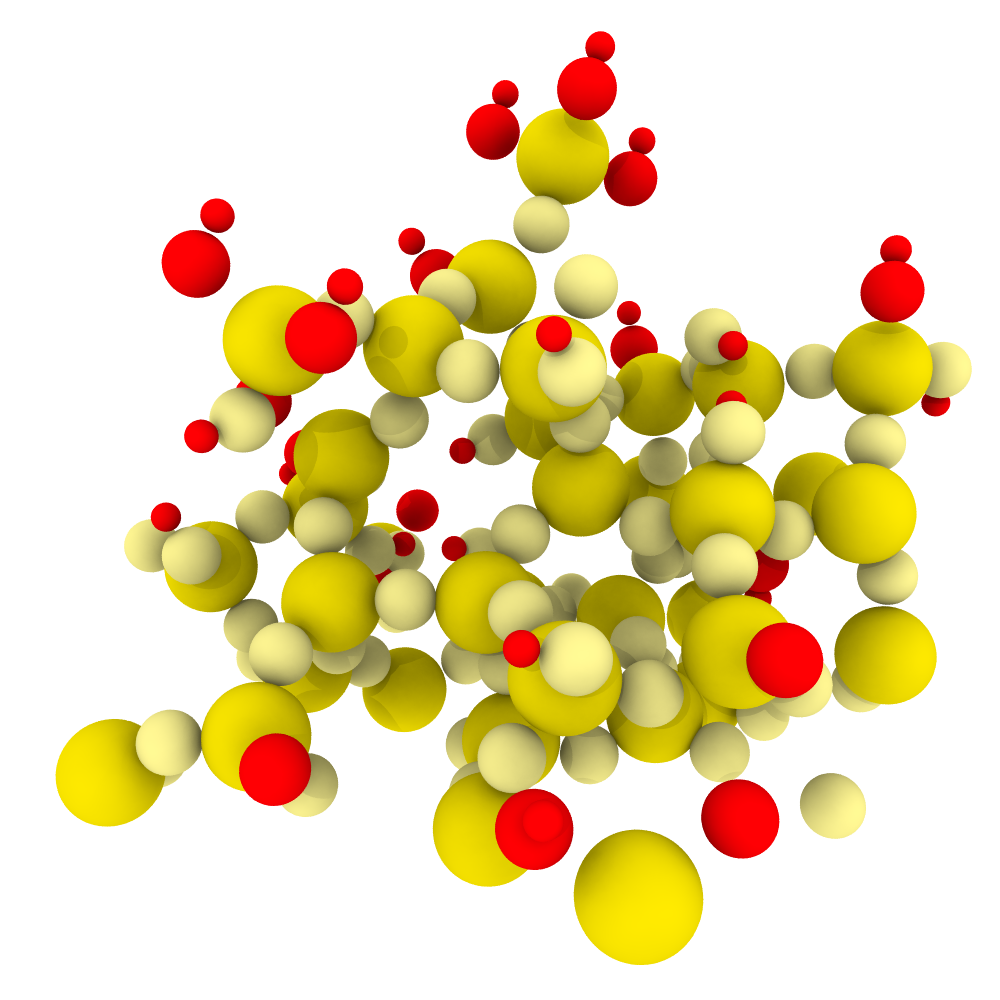
\includegraphics[width=0.7\textwidth]{images/passivation/passivation_example04.png}%
    \caption{
        Example of the result of the passivation procedure. Here the oxygen and hydrogen molecules are red, silicon atoms are yellow, and silicon-oxygen atoms are light yellow.%
    }%
    \label{fig:passivation_example}%
\end{figure}%

A good measure of the performance of the passivation method is the surface density of silanol after passivation. This number is often called the \emph{silanol number}, and us considered to be a physico-chemical constant, with a numerical value $\alpha_\text{OH} = 4.6$ (least-squares method) and $\alpha_\text{OH}\text{ nm}^{-2}$ (arithmical mean) \cite{zhuravlev1999silanol}, and is known in literature as the Kiselev-Zhuravlev constant. As we will see, measuring the surface area of porous system is not trivial, so estimating this density is not trivial. But by creating a completely flat pore and passivating it, we found that we got a silanol surface density between 4 and 7 nm$^{-2}$, depending on how we measure the surface area of the pore, and how we cound the number of silanol groups. % $\approx 7.05\text{ nm}^{-2}$ (if counting number of inserted hydrogen atoms) or $\approx 3.53\text{ nm}^{-2}$ (if counting number if inserted oxygen atoms). MAYBE MEASURE THIS PROPERLY?

% \todobo{Decide on whether to include silanol density stuff, and if so, write it}
% \orangebox{
% A good measure of the performance of the passivation method is the surface density of silanol after passivation. This number is often called the \emph{silanol number}, and us considered to be a physico-chemical constant, with a numerical value $\alpha_\text{OH} = 4.6$ (least-squares method) and $\alpha_\text{OH}\text{ nm}^{-2}$ (arithmical mean) \cite{zhuravlev1999silanol}, and is known in literature as the Kiselev-Zhuravlev constant. As we will see, measuring the surface area of porous system is not trivial, so estimating this density is not trivial. But by creating a completely flat pore and passivating it, we found that we created a silanol surface density of $\approx 7.05\text{ nm}^{-2}$ (if counting number of inserted hydrogen atoms) or $\approx 3.53\text{ nm}^{-2}$ (if counting number if inserted oxygen atoms). MAYBE MEASURE THIS PROPERLY?

% If the big number (7): since we inserted neutrally, the excess atoms will diffuse into the water anyway
% If the small number: the water we inject later will passivate the rest of the atoms
% Could also be caused by how we cut??
% The surface area is really bigger than $L^2$, since the atoms make a ``rough'' surface, not flat.
% }
        \FloatBarrier
        \section{Injecting water}
After removing atoms to create a fracture, and passivating the system, we are now ready to inject water into the fracture. To do this we use the technique of \emph{voxelation} (see \cref{sec:voxelation}). We first divide the system into voxels, find the voxels that make up the void, and then put water molecules in these voxels. The water density can then be controlled by the size of the voxels we use, and how many of the voxels we fill.

% \orangebox{
% \begin{itemize}
%     \item This could/should have been done using grand canonical ensemble / grand canonical monte carlo -- but this is computationally heavy?
%     \item The voxelation technique has problems in thin and/or skewed pores (not horizontal/vertical)
%     \item We want to have a water phase that is realistic (can be realistic with low or high density and pressure) and liquid
% \end{itemize}
% }

\subsection{Finding correct voxel size}
If we want to inject water with density $\rho$% [kg/m$^3$]
, we can find the voxel size we need from the molar mass of water, $M_\text{H$_2$O} = M = 0.0180158 \text{ kg/mol}$. We use the molar mass and wanted density to find the ``volume'' each water atom should occupy% , the unit used in the \hl{MD integrator/program and output files}
, as follows
\begin{align*}
    V 
    = \frac{ M\text{ [kg/mol]} \times \dfrac{1}{N_A \text{ [mol$^{-1}$]}}}{ \rho\text{ [kg/m$^3$]} } 
    = \frac{M}{\rho N_A}\text{[m$^3$]}
\end{align*}
where $N_A$ is the Avogadro constant. From here we find the size of the voxels by taking the cube root
\begin{align}
    l = \left(\frac{M}{\rho N_A} \right)^{1/3}\text{ m}.
    \label{eq:inject_water_voxel_size}
\end{align}
To get a water density approximately equal to $\rho$ we can then use a voxel size $l$, and put one water atom in each voxel. If we for example want to insert water with $\rho = 1000\text{ kg/m}^3$, approximately the density of water in room temperature, we get a voxel size of
\begin{align*}
    l = \left(\frac{0.0180158 \text{ kg/mol}}{1000\text{ kg/m$^3$} \times 6.0221 \times 10^{23}\text{ mol$^{-1}$}} \right)^{1/3} = 3.1 \text{ \AA}.
\end{align*}

\subsubsection{Voxel size in finite systems}
Since we have a finite system we usually can not use the exact voxel size we want, but we have to divide the system into an integer number of voxels. This means that we will not get the exact density we want if we fill all voxels. To remedy this we only fill the fraction of voxels to get the wanted density.

In practice we use the following procedure
\begin{itemize}
    \item Find the number of voxels to divide the system into (in each direction) via
    \begin{align*}
        n_i = \left\lceil \frac{L_i}{l_i} \right\rceil,
    \end{align*}
    where $L_i$ is the system size in dimension $i$ and $l_i$ is the voxel size calculated using \cref{eq:inject_water_voxel_size}. We use the ceiling-function to ensure that the actual voxel size we use is smaller than (or equal to) the voxel size we calculated. We find the actual voxel size via
    \begin{align*}
        \tilde l_i = \frac{L_i}{n_i}.
    \end{align*}
%     \item Mark all voxels within \hl{what radii?} as occupied.
    \item Divide the system into voxels of size $(\tilde l_x, \tilde l_y, \tilde l_z)$, and find the voxels that make up the void (see \cref{sec:inject_water_find_empty_voxels} for more on this).
    \item To find the ratio of voxels to put water molecules in we first calculate the density we would get if we filled all empty voxels using
    \begin{align*}
        \tilde\rho = \frac{M}{\tilde l_x \tilde l_y \tilde l_z N_A},
    \end{align*}
    and then find the number of voxels to fill as
    \begin{align*}
        \tilde N = N\frac{\tilde\rho}{\rho} = N\frac{\tilde l_x \tilde l_y \tilde l_z}{l_x l_y l_z},
    \end{align*}
    where $N$ is the total number of empty voxels.
    %\item \hl{Put a water molecule $\tilde N$ voxels}. 
    
    This can for example be done by looping over all voxels, drawing a random uniform number between 0 and 1 for each voxel, and putting a molecule in the voxel if the random number is smaller than $\tilde N / N$.
%     \begin{listing}[!htb]%
%         \begin{cppcode*}{gobble=12}
%             for (int i = 0; i < voxels.size(); i++)
%             {
%                 if (rand() < n_voxels_to_fill/n_voxels)
%                 {
%                     voxels[i].push_back(create_random_water_atom());
%                 }
%             }
%         \end{cppcode*}
%     \caption{%
%         \hl{FINISH THIS LISTING}.%
% %         \label{list:sampling}%
%     }%
%     \end{listing}%
\end{itemize}
The water molecules are inserted with the oxygen atom in the center of the voxel, and the two hydrogen atoms pointing in a random direction, but with an angle of $\sim 104.45^\circ$.

% \subsection[Finding empty/unoccupied voxels]{Finding \hl{empty/unoccupied} voxels\label{sec:inject_water_find_empty_voxels}}
\subsection{Identifying the voxels that make up the void\label{sec:inject_water_find_empty_voxels}}
The naive way of finding the voxels to fill with water is to just find which voxel each silicon and oxygen atom is in, and mark those as occupied. Using this method we found that we often got some empty voxels inside the silica matrix, which meant we got single water atoms trapped inside what was supposed to be the silica matrix. This is most likely cause by the amorphous structure of silica in the glass state, in which there are small pores spread throughout the structure.

% This can be explained if we compare the voxel size of $3.1 \text{ \AA}$ in water with a density of $\rho = 1000\text{ kg/m$^3$}$, as we found above, to the typical  bond length between silica tetrahedra in solid silica, which is about \hl{???}. When we take into account the amorphous structure of silica we see that it is likely that we get some small pores with room for a water atom in between some of the silica tetrahedra.\todoao{better explanation}

To solve this we assign a radius to each atom type, and mark all voxels with the center of the voxel within this radius from an atom as occupied. The rest of the voxels should now be a good approximation to the void. See \cref{fig:inject_empty_voxel} for an illustration of this procedure. 
%
\begin{figure}[htpb]%
    \centering%
    \begin{subfigure}[b]{0.45\textwidth}%
        \includesvg[width=\textwidth, svgpath=./images/inject_water/]{drawing02}%
%         \caption{}%
        \caption{Marking only one voxel per atom as occupied.}%
%         \label{fig:pass_tet01}%
    \end{subfigure}%
    \hspace{0.05\textwidth}%
    \begin{subfigure}[b]{0.45\textwidth}%
        \includesvg[width=\textwidth, svgpath=./images/inject_water/]{drawing_radius02}%
%         \caption{}%
        \caption{Marking all voxels within radius from atom as occupied.}%
%         \label{fig:pass_tet02}%
    \end{subfigure}%
    \caption[
        To find voxels that make up the void/pore in we can either \textbf{a)} mark the voxel each existing atom belongs in as occupied, or \textbf{b)} mark all voxels within a radius from each atom as occupied. We can assign a different radius to each atom. We have illustrated using part of a silica tetrahedra, with one silicon atom (the large blue dot) and two oxygen atoms (the smaller red dot). The center of each voxel is marked by a dot 
    ]{%
        To find voxels that make up the void/pore in we can either \textbf{a)} mark the voxel each existing atom belongs in as occupied, or \textbf{b)} mark all voxels within a radius from each atom as occupied. We can assign a different radius to each atom. We have illustrated using part of a silica tetrahedra, with one silicon atom (
\includegraphics[scale=0.8]{./images/inject_water/silicon.pdf}) and two oxygen atoms (\raisebox{0.3ex}{
\includegraphics[scale=0.8]{./images/inject_water/oxygen.pdf}}). The center of each voxel is marked by a dot. %
        %\hl{Maybe change to v01 of images?} \hl{This voxel size is pretty tiny...}%
    }%
    \label{fig:inject_empty_voxel}%
\end{figure}%

A different solution to the problem of tiny pores inside the silica matrix is to remove all small clusters of voxels (where a ``small cluster of voxels'' would need to be defined), or perhaps to use different voxel sizes for finding the void and filling the void with water.

% \orangebox{
% \begin{itemize}
%     \item Remove tiny pores?
%     \item Give voxels random velocity based on wanted temperature? Now using zero!
%     \item Mark all voxels within distance from other atoms as occupied
%     \item Fill other voxels with H2O with random O-H orientation, but correct angle
%     \item Improvement: Use one voxel size in the beginning (to avoid one-voxel pores), and then use a smaller voxel size when injecting water
% \end{itemize}
% }


    \chapter{Measurements}
% \section{Voxelation, calculating distances, finding neighbors, neighbor lists, periodicity tricks\label{sec:voxelation}}
% \section{}
%
%

\todob{intro here?}








% \FloatBarrier
% \section{``Voxel counter''}
% \todob{Write about voxel counter}
% \todod{Voxel counter code example?}
%     A histogram of the fraction of voxels that has one or more atom in them vs. the voxel size in x-, y-, and z-direction.
%     
% % \FloatBarrier
% \section{Cage cage correlation}
%     \todod{Measure cage cage correlation}
% 
% % \FloatBarrier
% \section{Surface area of pores}
%     Only one large pore in my system, so not useful?

        \section{Distance to silica matrix\label{sec:measuring_distance_to_matrix}}
% \todoao{Why measure as function of distance to matrix}%
% \todoa{Finish measuring as function of distance from matrix}
% Mean distance from matrix in range --> if we limit the standard deviation as well, we're effectively limiting temperature, or diffusion??
% When measuring things like density, diffusion, and the tetrahedral order parameter in a nanoporous system, we often want to study the behaviour of 
To study the water-silica interface we want to do measures as function of the distance to the surface of the pore, in our case meaning the distance from a water molecule to the interface between water and silica. The first problem with this is to find out how to measure the distance from a point, for example a water molecule, to the surface. Most of our measures are done on water molecules in fractures and pores, so we first define the position of the water molecule as equal to the position of the oxygen atom in the water molecule. We then use the distance from these water-oxygen atoms to the nearest silica atom to define a distance from the water molecule to the surface of the silica matrix. Finding the nearest silica atom is not trivial though, so a separate procedure for doing this is shown in \cref{sec:find_distance_to_surface}.

When measuring quantities that only depend on data from one timestep we do not have to worry about that the atoms move, so we just sort the atoms by distance to the surface using the procedure in \cref{sec:find_distance_to_surface} and do our measurements, individually on each timestep. But if we want to study for example diffusion, or the tetrahedral order parameter, which depend on data from several timesteps, we have to find a good way to define which atoms are in a certain range of the surface. We tried different methods, but ended up using the average distance to the surface for this.
%\todobo{why, examples of tested methods -- constant within bin --> bad statistics, low number of atoms}.

\subsection{Note on this method\label{sec:distance_to_matrix_issues}}
\todobo{Clean up ``distance to z'' stuff?}%
When we define the distance to the silica matrix as the distance to the nearest silicon atom, we get some effects we should take note of for atoms very close to the matrix. With our definition of the distance to the silica matrix we are effectively making our bins out of spherical shells centered on each silicon atom. Compared to for example using the $z$-distance to the surface in a completely flat fracture, where we know the $z$-height of the surface, we see that this can give different results. The problem is of course that in a random fracture in a silica system we can not easily define a normal vector to the surface of the fracture, so finding an equivalent to the $z$-distance in such a fracture is hard.

When we do our measurements as a function of distance to the silica matrix we usually sort the atoms into bins according to their (average) distance to the nearest silicon atom. At distances much larger than the average distance between the silicon atoms at the surface of the fracture this is not a problem, since the curature of the spherical shells is low, and the volume enclosed by the shells is pretty close to the one we would have gotten if we had created bins used $z$-positions in flat fracture. But at distances close to the average distances between the silicon atoms we begin to see that the volumes our bins consist of start curving around the silicon atoms, instead of staying flat as they would have if we were using the $z$-distance. See \cref{fig:distance_to_matrix_illustration} for an illustration of this. In this illustration we have illustrated bins created using the same bin width and distance from the matrix, using the two different methods. The dark gray areas are the ones that are included using both methods ($A_\text{Si}\cap A_z$), the light grey areas ($A_\text{Si}$) are the ones unique to the spherical shell bins, and the yellow areas are the ones unique to the the $z$-distance bins ($A_z$).%
%
\begin{figure}[htb]%
% \centering%
    \begin{minipage}[c]{0.6\textwidth}%
        \captionsetup{width=0.925\textwidth}%
        \centering%
        \includesvg[width=\textwidth, svgpath=./images/density/]{number_of_molecules_all_distances02}%
        \caption{%
            Plot of the number of atoms in each bin, when using the distance to the nearest atom for binning.%
            \label{fig:distance_to_matrix_number_of_atoms}%
        }%
    \end{minipage}%
    \hfill%
    \begin{minipage}[c]{0.3999\textwidth}% % change "b" to "t" to anchor top instead of bottom
%         \captionsetup{width=0.95\textwidth}% % minipage defines a \textwidth for it's own, so we have to repeat this command inside the minipage
        \captionsetup{width=0.9\textwidth}% % minipage defines a \textwidth for it's own, so we have to repeat this command inside the minipage
        \centering%
        \includesvg[pretex=\normalsize, width=0.9\textwidth, svgpath=./images/distance_to_matrix_illustration/]{figure12}%
        \caption{%
            Illustration of binning when using distance to nearest silicon atom as definition of distance to silica matrix ($r_\text{Si})$, vs. $z$-distance ($r_z$).%
            \label{fig:distance_to_matrix_illustration}%
        }%
    \end{minipage}%
\end{figure}%

This difference in binning is something we should be wary about when comparing our results to measurements done using the $z$-distance as the distance to the matrix. One result of this can be seen in \cref{fig:distance_to_matrix_number_of_atoms}, where we have plotted the number of atoms in each bin of width $0.25\text{ \AA}$ against the distance from the silica matrix (meaning the radius of the spherical shells). We see that we get no atoms in the bins from 2 to 3 \Ang, but a big spike just below 2 \AA. This spike is most likely caused by water-oxygen atoms that are bound to silicon atoms, which we placed there when passivating the system (silicon-water atoms from the initial silica crystal are not included in the counting, but we use water-oxygen when passivating). If we had used the $z$-distance in a flat fracture in a system like this, we would most likely have gotten a very different distribution below 4 \AA, with a more flat distribution instead of it going to zero, since the angular distribution of the oxygen atoms around the silica atoms makes the $z$-distance vary.
        \section{Voxelation\label{sec:voxelation}}
The method of voxelation is a method where we divide our simulation system into adjacent boxes or \emph{voxels} (3-dimensional pixels). The system is divided into $n_x\times n_y\times n_z$ voxels of size $l_x\times l_y\times l_z$. Depending the what we want to calculate we can calculate the voxel size from the number of voxels, or vice versa, using the following relation
\begin{align*}
    n_i = \frac{L_i}{l_i},
\end{align*}
where $L_i$ is the system size, and we assume that the voxel size $l_i$ is set so that $L_i$ is evenly divisible by $l_i$ (meaning that the remainder of $L_i/l_i$ is zero). If we have a maximum or minimum voxel size $l_i^\text{max}$ or $l_i^\text{min}$ we can use the following relations to calculate the number of voxels
\begin{align*}
    &n_i=\left\lfloor\frac{L_i}{l_i^\text{max}}\right\rfloor &\text{or}& &n_i=\left\lceil\frac{L_i}{l_i^\text{min}}\right\rceil,
\end{align*}
where $\lfloor x \rfloor$ is the \Verb!floor!-function and $\lceil x \rceil$ is the \Verb!ceil!-function.

The voxels are indexed $(i,j,k)$ where $i,j,k \in [0,n_i-1]$, and a voxel is defined as the points $(x,y,z)$ where
\begin{align}
    \left\lfloor\frac{x}{l_x}\right\rfloor = i,\label{eq:find_voxel_index}
\end{align}
and similarly for the other dimensions.

\subsection{Neighbor lists\label{sec:neighbor_lists}}
When doing calculations and measurements on a molecular system, we often need information about the neighboring atoms of each atom, and we want to make a so-called \emph{neighbor list}, which are lists of which atoms are within a distance $dr$ of each atom. Finding out which atoms are within a certain distance of each atom can take a long time; the trivial way of checking each atom against all other atoms scales as $\mathcal{O}(N^2)$, $N$ being the number of atoms. 
%
%There are many clever algorithms for finding nearest neighbors, often called a ``nearest neighbor search'' (see \url{http://www.slac.stanford.edu/cgi-wrap/getdoc/slac-r-186.pdf} and references in that paper, especially ``11. Levinthal 1966''). 

Since we want to find all neighbors within a distance $dr$ of a point, for all or most of the atoms, we can use the voxelation method to do it efficiently. To do this we first voxelate the system using a minimum voxel size equal to $r$. We then find which voxel each atom belongs to, and store this. We can then find the atoms within a distance $dr$ from a point $(x,y,z)$ by first finding the voxel this point lies in using (from \cref{eq:find_voxel_index})
\begin{align*}
    &i = \Bigg\lfloor \frac{x}{l_x} \Bigg\rfloor,& &j = \Bigg\lfloor \frac{y}{l_y} \Bigg\rfloor,& &j = \Bigg\lfloor \frac{z}{l_z} \Bigg\rfloor,&
\end{align*}
where $l_x\times l_y \times l_z$ is the actual voxel size (we need an even number of voxels, so the actual voxel size is governed by the system size). We then check the distance between the point and the atoms in the voxel the point belongs in, and the atoms in the 26 neighboring voxels of this voxel. 
% \todoco{make voxel size vs. $dr$ illustration}%

Checking the 26 neighboring voxels ensure that we included all atoms within the distance $dr$. We can see this by looking at the worst case example, where we have a point right at the edge of the voxel it belongs to, at $(i+(1-\epsilon_0))$, and an atom in voxel $(i+2)$ being as close to the point as possible, at $(i+2 + \epsilon)$. The distance between those two points would then be
\begin{align*}
    ((i+2)l + \epsilon_1) - (il + (l-\epsilon_0)) 
    &= ((i + 2) - (i + 1) - \epsilon_0)l + \epsilon_1 + \epsilon_0 \\
    &= l + \epsilon + \epsilon_0,
\end{align*}
which is larger than $l$, since $\epsilon_0, \epsilon_1$ have to be larger than 0.

When voxelating the system using the distance $r$ we should take care not to use a too small distance, i.e. make the voxels too small and create a lot of voxels. Since the total number of voxels goes as $n^3$ the memory needed to store the matrix increases rapidly with decreasing voxel size. To avoid this we usually implement a hard limit to the number of voxels, and found that a limit of $n < 256$ or even $n < 128$ seemed to work good in most cases. On the other hand, if we make the voxels too large we soon find that the program is not especially efficient. This is because most voxels will have a lot of atoms in then, and we have to look through a lot of atoms when checking the 26+1 voxels for each atom.

An implementation of the voxelation method for creating neighbor lists can be seen in \cref{list:create_neighbor_lists}. Note that when calculating distances between points we usually calculate and compare squared distances like $r^2 = (x_1-x_2)(x_1-x_2) + \dots$, since calculating roots are a time-consuming operation on a computer (at least compared to multiplication and addition).
%
% We did not find any algorithms for solving this specific problem, and the usual algorithms can not benefit from the fact that we need to find the nearest neighbors of \emph{all} points.
%
\begin{listing}[!htb]%
\begin{cppcode*}{gobble=4}
    int nVoxels = floor(systemSize/radius);
    double voxelSize = systemSize*nVoxels;
    
    sortAtomsIntoVoxels(atoms, voxelSize, voxels);
    
    vector<vector<Atom*> > neighborAtoms(atoms.size());
    
    // Loop over all atoms
    for (Atom *atom : atoms) {
        // Index of the voxel this atom belongs to
        ivec3 index = floor(atom.position() / voxelSize)
        
        // Loop over all 27 neighbor voxels (including self)
        for (int di = -1; di <= 1; di++)
        for (int dj = -1; dj <= 1; dj++)
        for (int dk = -1; dk <= 1; dk++)
        {{{
            // Index of neighbor voxel using periodic boundary conditions
            // nx, ny, nz is the number of voxels in each direction
            int i = (index[0] + di + nx) % nx;
            int j = (index[1] + dj + ny) % ny;
            int k = (index[2] + dk + nz) % nz;
            
            neighborAtoms[atom.index()].push_back(
                findAtomsWithinRadius(atom, voxels[i][j][k], radiusSquared)
            );
        }}}
    }
\end{cppcode*}
\caption{%
    An example of how to find the neighbor atoms within a given distance (\mono{radius}) of all atoms. This example assumes a cubic system of size \mono{systemSize}. See \cref{list:sortAtomsIntoVoxels,list:findAtomsWithinRadius} for example implentations of \mono{sortAtomsIntoVoxels} and \mono{findAtomsWithinRadius}. %
    \label{list:create_neighbor_lists}%
}%
\end{listing}%
%
\begin{listing}[!htb]%
\begin{cppcode*}{gobble=4}
    void sortAtomsIntoVoxels(
        const vector<Atom*> &atoms, 
        double voxelSize, 
        vector<vector<vector<Atom*> > > &voxels) {
        
        for (Atom *atom : atoms) {
            // Index of the voxel this atom belongs to
            int i = floor(atom.position().x() / voxelSize);
            int j = floor(atom.position().y() / voxelSize);
            int k = floor(atom.position().z() / voxelSize);
            voxels[i][j][k].push_back(atom);
        }
    }
\end{cppcode*}
\caption{%
    Example of implementation of \mono{sortAtomsIntoVoxels} from \cref{list:create_neighbor_lists}, for sorting atoms into voxels with size \mono{voxelSize}. We use the \mono{floor} function to get the index of the voxel each atom belongs in, using zero-based numbering. % \mono{sortAtomsIntoVoxels}. %
    \label{list:sortAtomsIntoVoxels}%
}%
\end{listing}%
\begin{listing}[!htb]%
\begin{cppcode*}{gobble=4}
    vector<Atom*> findAtomsWithinRadius(
        Atom *atom1, const vector<Atom*> &voxel, double radiusSquared) {
        
        vector<Atom*> neighborAtoms;
        
        // Loop over atoms in neighbor voxel
        for (Atom *atom2 : voxel) {
            if (atom2 != atom1) {
                double drSquared = 
                    calculateDistanceSquaredBetweenAtoms(atom1, atom2);
                if (drSquared < radiusSquared) {
                    neighborAtoms.push_back(atom2);
                }
            }
        }
        return neighborAtoms;
    }
\end{cppcode*}
\caption{%
    Example implementation of \mono{findAtomsWithinRadius} from \cref{list:create_neighbor_lists}. See \cref{list:calculateDistanceSquaredBetweenAtoms} for an example implementation of \mono{calculateDistanceSquaredBetweenAtoms}.%
    \label{list:findAtomsWithinRadius}%
}%
\end{listing}%
%
\begin{listing}[!htb]%
\begin{cppcode*}{gobble=4}
    double calculateDistanceSquaredBetweenAtoms(Atom *atom1, Atom *atom2) {
        vec3 dr = atom2->position() - atom1->position();
        
        // Minimum image convention
        for (int dim = 0; dim < 3; dim++) {
            if      (dr[dim] >  L[dim]/2.0) dr[dim] -= L[dim];
            else if (dr[dim] < -L[dim]/2.0) dr[dim] += L[dim];
        }
        
        // Calculate $dr^2$ instead of $\sqrt{dr^2}$, since sqrt() is a very 
        // slow operation, and in this case is unnecessary
        return dr.lengthSquared();
    }
\end{cppcode*}
\caption{%
    Example implementation of \mono{calculateDistanceSquaredBetweenAtoms} from \cref{list:findAtomsWithinRadius}.%
    \label{list:calculateDistanceSquaredBetweenAtoms}%
}%
\end{listing}%

\subsection{Finding distance to surface\label{sec:find_distance_to_surface}}
When doing measurements on water molecules we often want to know the distance from the water molecule to the surface of the pore the water molecule is in. To find this we first define the position of the water molecule as the position of the oxygen atom in the molecule. We then use the distance between this oxygen atom to the nearest silicon atom as the distance to the surface.

To use the voxelation method we need to have a maximum distance to look for silicon atoms in. This atom should be set as small as possible, to efficiently use the voxelation method\footnote{We usually implement a hard upper bound on the number of voxels, or a lower bound on the voxel size, to keep the memory consumption of our program in check.}. We divide the system into voxels using the technique from \cref{sec:voxelation}, and sort all silicon atoms into the voxels. For each water-oxygen atom we then find the distance to the nearest silicon atom by calculating the distance between the oxygen atom and the silicon atoms in the voxel the oxygen atom belongs in, and the silicon atoms in all 26 neighbor voxels. See \cref{sec:neighbor_lists} for more details.

        \FloatBarrier
        \section{Density}
To measure the density in a uniform system consisting of just one atom type, we can use
\[
    \rho = \frac{Nm}{V},
\]
where $N$ is the number of atoms, $m$ the mass of an atom, and $V$ the volume of the whole system. But if we have a more complicated system, like in our case where we have three different atom types, liquid water in some parts of the system, and solid silica in other parts, we can not use that simple relation. What we do instead is to assiociate a volume $V_i^j$ with each atom of type $j$, and calculate the density of atom type $j$ using
\[
    \rho_j = \dfrac{m_jM}{\sum_{i=0}^M V_i^j},
\]
where $m_j$ is the mass an atom of type $j$, and $M$ is the number of atoms of type $j$. We identify as the $\rho_j/m_j$ number density. We can find the mass of an atom type from standard tables of molar masses, but we still need to find the volumes $V_i^j$ associated with each atom. To do this we use something called Voronoi cells and the process of Voronoi tesselation. Voronoi tesselation is done by dividing the system into non-overlapping convex polyhedra (or convex polygons in 2 dimensions), with one atom in each polyhedra. The volume inside the polyhedron surrounding each atom consists of all points in space closer to that atom than any other atom. 

We use the \cpp-library \texttt{Voro++} to find the Voronoi cells, and calculate the volumes of the cells. See \cref{fig:2d_voronoi_diagram} for an illustration of a 2-dimensional Voronoi, and \cref{fig:3d_voronoi_diagram} for a rendering of a 3D Voronoi diagram.
%
\begin{figure}[htpb]%
% \centering%
    \begin{minipage}[t]{0.485\textwidth}%
        \captionsetup{width=\textwidth}%
        \centering%
%         \includesvg[width=0.8\textwidth, svgpath=./images/voronoi/]{2d_diagram03}%
        \includesvg[height=0.7\textwidth, svgpath=./images/voronoi/]{2d_diagram06_overlapping}%
        \caption{%
            Illustration of Voronoi cells in 2 dimensions. Freely after Wikipedia Commons\cite{wikiVoronoiImage}.%
            \label{fig:2d_voronoi_diagram}%
        }%
    \end{minipage}%
    \hfill%
    \begin{minipage}[t]{0.485\textwidth}% % change "b" to "t" to anchor top instead of bottom
    \captionsetup{width=\textwidth}% % minipage defines a \textwidth for it's own, so we have to repeat this command inside the minipage
        \centering%
%         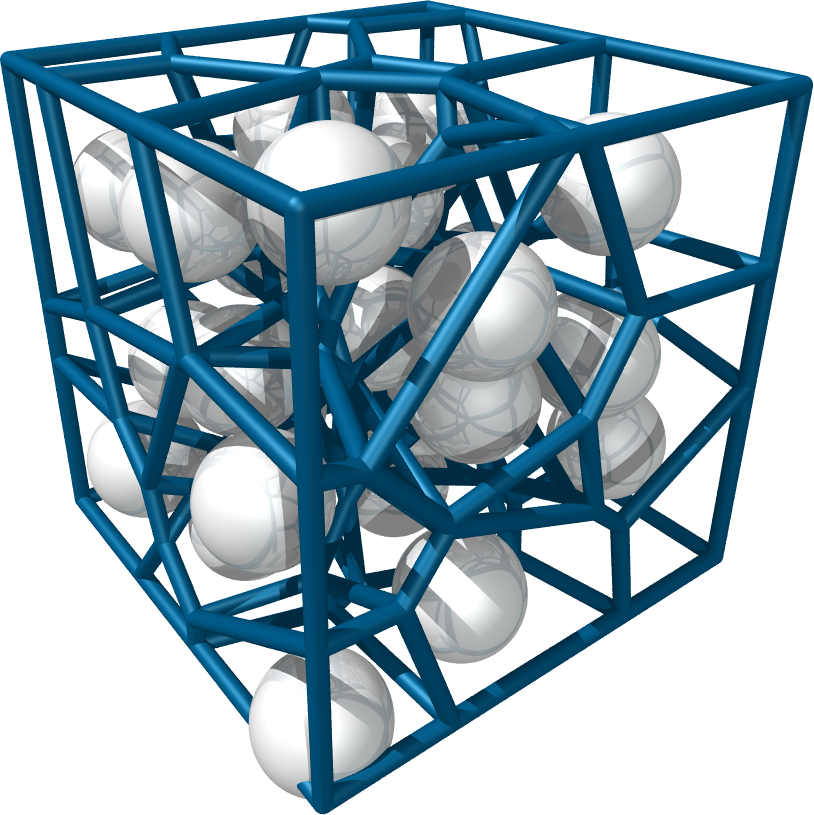
\includegraphics[width=0.8\textwidth]{images/voronoi/3d_diagram04_crop.png}%
        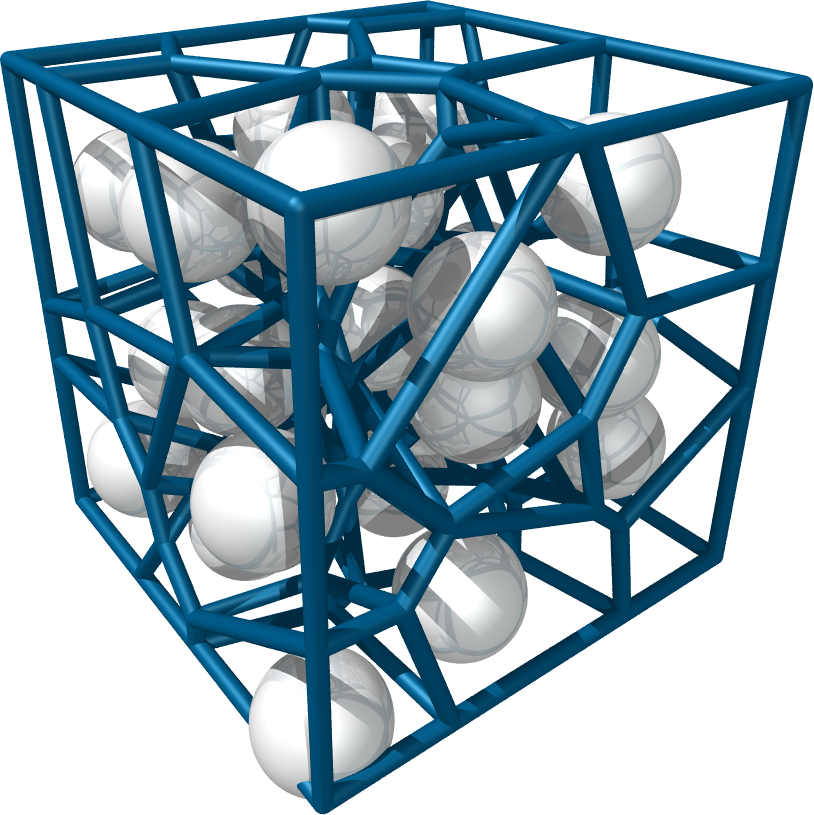
\includegraphics[height=0.7\textwidth]{images/voronoi/3d_diagram04_crop.png}%
        \caption{%
            Rendering of Voronoi cells in 3 dimensions, in a system of 27 particles. Voronoi cells created using the \cpp-library \texttt{Voro++}\cite{rycroft2009voro,webvoro++}, and rendered using the program \texttt{povray}\cite{webpovray}. %
            \label{fig:3d_voronoi_diagram}%
        }%
    \end{minipage}%
\end{figure}%

\todoa{Something about removing hydrogen atoms, and just use oxygen position as hydrogen position, and water atom ``volume''? This simplifies life for us, since we do not have to find which water molecule each hydrogen atom belongs to, but we could get inconsistent water density. But since we use the same method for all measurements, we can compare relative densities.}

% \todoao{Write about averaging over timesteps and atoms}

\todoao{Something about removing extreme points/tail in distribution? Caused by vacuum.}
        \section{Diffusion}
\todob{derivation of diffusion? See \cite[Section~4.4.1]{frenkel2001understanding}}
When we talk about diffusion in this thesis we mean the process of \emph{self-diffusion}, which is different from ``normal'' diffusion, which is the net movement of a substance in the presence of a gradient, which can be for example a concentration gradient, a temperature gradient, or a pressure gradient. With \emph{self-diffusion} we mean the random movement in a substance that has no gradients.

Diffusion can be characterized by a constant $D$, which is related to the displacement of each atom relative to a initial position. We can measure this constant by measuring the mean square displacement $r_i^2(t)$ of each atom as a function of time, and average over all atoms. The mean square displacement is measured as
\begin{align*}
    \Braket{r^2(t)} = \frac{1}{N} \sum_{i=1}^N \left( \rvec_i(t) - \rvec_i(t=0) \right)^2,
\end{align*}
where $\rvec_i(t=0)$ is the initial position of atom $i$. From theoretical considerations of the diffusion process we can relate the diffusion constant to the mean square displacement through\cite[Section~4.4.1]{frenkel2001understanding}
\begin{align}
    \lim_{t\rightarrow \infty}\dpd{}{t}\Braket{r^2(t)} = 2dD\label{eq:diffusion_derivative}
\end{align}
where $d$ is the spatial dimension. This means that we can find the diffusion constant in a molecular dynamics simulation by measuring the mean square displacement for many timesteps, and find the slope of this data as the diffusion constant in the limit $t\rightarrow \infty$. We are limited in that we ca not actually simulate infinite number of timesteps, but have to find a reasonable number of timesteps to measure over. An example of how to sample the mean square displacement $\Braket{r^2(t)}$ in a simulation can be seen in \cref{list:diffusionSample}.
%
% This means that we can find the diffusion constant in a molecular dynamics simulation by measuring the mean square displacement for many timesteps, and plotting $\Braket{r^2(t)}/(2dt)$ as a function of time. The diffusion constant will then be the value this expression approaches when simulating for enough timesteps.
%
%An example of how to measure the mean square displacement in a molecular dynamics \hl{simulation/program} as outlined in \cref{chap:simple_md_program} can be seen in \cref{list:diffusionSample}.
% Fick's law relates flux $\bvec j$ of diffusing species to the concentration gradient $\bvec \nabla c$ of the species
% \begin{align*}
%     \bvec j = -D\bvec \nabla c,
% \end{align*}
% where $D$ is the proportionality constant called the diffusion \hl{coefficient/constant}.
% 
% Conservation of \hl{species/atoms?}
% \begin{align*}
%     \dpd{c(r,t)}{t} + \div \cdot \vec j(r,t) = 0,
% \end{align*}
% which gives
% \begin{align}
%     \dpd{c(r,t)}{t} - D\nabla^2 c(r,t) = 0.
%     \label{eq:diffusion_diff}
% \end{align}
% % We can solve this equation with the boundary condition
% % \begin{align*}
% %     c(r,0) = \delta (r),
% % \end{align*}
% % where $\delta(r)$ is the Dirac delta function, which gives
% % \begin{align*}
% %     c(r,t) = \frac{1}{(4\pi Dt)^{d/2}} \exp\left(-\frac{r^2}{4Dt}\right).
% % \end{align*}
% By multiplying \cref{eq:diffusion_diff} by $r^2$ and integrating over all space we get
% \begin{align*}
%     \dpd{}{t}\int \drvec~ r^2 c(r,t) = D\int \drvec~ r^2 \nabla^2 c(r,t).
% \end{align*}
% We recognize the integral on the left-hand side as the the mean square displacement %\hl{time dependence of the second moment of $c(r,t)$???}
% \todo{what???}
% \begin{align*}
%     \int \drvec~ c(r,t) r^2 \equiv \Braket{r^2(t)},
% \end{align*}
% where we have imposed
% \begin{align*}
%     \int \drvec~ c(r,t) = 1.
% \end{align*}
% Applying partial integration to the right-hand side we obtain
% \begin{align*}
%     \dpd{\Braket{r^2(t)}}{t} 
%     &= D\int \drvec~ r^2 \nabla^2 c(r,t) \\
%     &= D\int \drvec~ \div \cdot \left(r^2\nabla c(r,t)\right) - D\int\drvec~ \div r^2 \cdot \nabla c(r,t) \\
%     &= D\int \dif \vec S~ \left(r^2\div c(r,t)\right) - 2D\int\drvec~ \rvec \cdot\div c(r,t) \\
%     &= 0 - 2D\int\drvec~ (\div \cdot \rvec c(r,t)) + 2D\int\drvec~ (\div \cdot \rvec) c(r,t) \\
%     &= 0 + 2dD\int \drvec~ c(r,t) \\
%     &= 2dD
% \end{align*}
% 
% 
% \begin{align*}
%     \dpd{\Braket{r^2(t)}}{t} = 6D
% \end{align*}
% $\Rightarrow$ Plot mean square distance as function of time
% \begin{align*}
%     \Braket{\delta r(t)^2} = \frac{1}{N} \sum_{i=1}^N \delta \rvec_i(t)^2
% \end{align*}
% and find $6D$ as slope of plot \hl{(after a while?)}
%
\begin{listing}[!htb]%
\begin{cppcode*}{gobble=4}
    double diffusionSample(System &system) {
        double rSquared = 0.0;
        for (Atom *atom : system.atoms()) {
            drVec = atom->positiom() - atom->initialPosition() 
                    + atom->getBoundaryCrossings()*system.size();
            rSquared += drVec.lengthSquared();
        }
        rSquared /= system.nAtoms();
        return rSquared;
    }
\end{cppcode*}
\caption{%
    An example of how to calculate the mean square displacement in a molecular dynamics simulation. Example implementation of \mono{diffusionSample} from \cref{list:sampling}. We store the inital positions of the atoms as \mono{atom->initialPosition()}, and when using periodic boundary conditions we count the number of times we have to translate the atom one system-size in each direction, so while the position of the atom will always be inside the system, the \emph{actual} position of the atom can be calculated by adding \mono{atom->getBoundaryCrossings()*system.size()} to $\rvec$.%
    \label{list:diffusionSample}%
}%
\end{listing}%

% To improve our statistics when measuring the diffusion constant as function of distance to the surface of the pore we can use different time origins to get different samples. %
To measure $D$ we see from \cref{eq:diffusion_derivative} that we have to let $t\rightarrow \infty$, but in practice we usually see that the gradient of $\Braket{r^2(t)}$ usually have stabilzed near its final value after ${\sim} 5\text{ k}$ timesteps of 0.050 picoseconds. We can use this to get more samples for our measurements, by using different time origos. This technique involves using different initial positions for the atoms, from different timesteps in the simulation, and then finding $\Braket{r^2(t)}$ for $t_i\leq t\leq t_{i+n}$, where we $n$ is the number of timesteps we want to use for each time origo. We can in theory use overlapping intervals for $t$, but we chose to use adjacent, non-overlapping intervals. 

See \cref{fig:find_diff_const_example} for an example of how we find the diffusion constant as the gradient of $\Braket{r^2(t)}$, using different time origos.
%
% \todoao{Finish diffusion time origo stuff}
% \todoa{mention using average distance to matrix, procedure from \cref{sec:measuring_distance_to_matrix}}
% \todob{Plot of $r^2$ using standard settings ($dt$ = 20.67, 100 timesteps between states) to show approx how many origos we need to get stable gradient}
%
%
\begin{figure}[!htb]%
    \centering% 
    {
        \newcommand{\la}{\langle}%
        \newcommand{\ra}{\rangle}%
        \includesvg[width=0.8\textwidth, svgpath = ./images/diffusion/]{diffusion_constant_example02}%
    }
    \caption{%
        Illustration of how we find the diffusion constant, using two different time origos, with 40 timesteps of 0.050 picoseconds for each time origo. We find the diffusion constant as the gradient of $\langle r^2(t)\rangle/6$ for the 25 last timesteps for each origo. We then use the average of the gradients for each time origo as our approximation of $D$.%
        \label{fig:find_diff_const_example}%
    }%
\end{figure}%
% r_start = 0.0
% r_step = 0.25
% n_steps = 40
% folder_name_iterator_start = 0
% folder_name_step = 1
% folder_name_n_steps = 200
% 
% steps_per_origin = 40
%
%
% Diff const (gradient)
% 0.0295056927145
% 0.0495650040286
% 0.117231421271
% 0.0246869083899
% 0.0785722907501
% 0.156826102758

        \section{Tetrahedral order parameter}
% \todoa{Do we measure TOP for molecules or atoms?}%
% \todoa{Write about how we measure P(Q)?, since we measure probability/relative occurrence and not TOP as function of something}%
The tetrahedral order parameter\cite{errington2001relationship} is effectively a measure of how tetrahedral a set of four points are. The tetrahedral order parameter $Q$ for a point $k$ is calculated as follows%
\begin{align}
    Q_k = 1 - \frac{3}{8}\sum_i^3\sum_{j=i+1}^4 \left[ \cos \theta_{ikj} + \frac{1}{3} \right]^2,\label{eq:top_definition}
\end{align}%
%
% \begin{minipage}[c][4cm][c]{\textwidth}%
%     \begin{minipage}[c]{0.7\textwidth}%
%         \centering%
%         $Q_k = 1 - \frac{3}{8} \displaystyle\sum_i^3 \displaystyle\sum_{j=i+1}^4 \left[ \cos \theta_{ikj} + \frac{1}{3} \right]^2$%
%     \end{minipage}%
% %
%     \begin{minipage}[c]{0.25\textwidth}%
%         \centering
%         \includesvg[pretex=\normalsize, width=\textwidth, svgpath=./images/tetrahedral_order_parameter/]{tetrahedra02}%
%         \captionof{figure}{\label{hei}}
%     \end{minipage}%
%     
%     \begin{figure}[htpb]%
%         \includesvg[pretex=\normalsize, width=\textwidth, svgpath=./images/tetrahedral_order_parameter/]{tetrahedra02}%
%         \caption{a}%
%     \end{figure}%
%     
%     \caption{%
%         Illustration of the angles and molecules involved in the calculation of the tetrahedral order parameter. The \hl{blue} dots are molecules, in our case usually water molecules. We have the center molecule $k$, and \hl{its} four nearest neighbors. $\theta_{ikj}$ is the angle between molecule $i$, $k$ and $j$, as indicated by the \hl{orange} arc. \hl{FINISH CAPTION}. %
%         \label{fig:top_tetrahedra}%
%     }%
% \end{figure}%
% \end{minipage}%
% \captionof{figure}{alfa}
%
where $\theta_{ikj}$ is the angle %
%between two vectors from the main point, $k$, to point $i$ and point $j$, respectively, 
$i-k-j$ (with $k$ in the vertex of the angle) %
and the two sums go over the 6 possible angles $\theta$, between the main point and \hl{its} four nearest neighbors. See \cref{fig:top_tetrahedra} for an illustration of the angles and points involved in the calculation. If we have $Q = 1$ the four points are arranged in a perfect tetrahedron, with $\theta_{ijk} = 2\arctan(2\sqrt(2)) \approx 109.47$ for all 6 possible angles between the four points, and as the points move away from this arrangement $Q$ decreases following \cref{eq:top_definition} (negative $Q$-values are possible).
%
\begin{figure}[htpb]%
    \centering%
    \includesvg[pretex=\normalsize, width=0.3\textwidth, svgpath=./images/tetrahedral_order_parameter/]{tetrahedra02}%
    \caption{%
        Illustration of the angles and points involved in the calculation of the tetrahedral order parameter. The \hl{blue} dots are points, in our case usually water molecules. We have the center point $k$, and \hl{its} four nearest neighbors. $\theta_{ikj}$ is the angle between point $i$, $k$ and $j$, as indicated by the orange arc. \hl{FINISH CAPTION}. %
        \label{fig:top_tetrahedra}%
    }%
\end{figure}%

We use the tetrahedral order parameter for investigating the coordination of water molecules relative to other water molecules. When we lower the temperature in water below freezing the average $Q$ will \hl{approach 1/increas}, since ice has very high coordination. Liquid water also has high coordination caused by the hydrogen bonds, but much lower coordination than ice, so the distribution of $Q$-values are more spread out, with the mean lower than the mean for ice.

When we measure the tetrahedral order parameter we measure $Q$ for all water molecules, defining the position of the water molecules as the position of the oxygen atom in each molecule, and plot the \hl{relative occurrence}\todob{probability density?}, $P(Q)$, to investigate the distribution of $Q$-values. Since $Q$ is not dependent on several timesteps (like for example diffusion), averaging over several timesteps is trivial. \todobo{But we should be wary of correlations between states?}. Since silica is hydrophilic we expect $Q$ to be different for water molecules near the silica surface, so we will measure $P(Q)$ as function of distance to the silica matrix.

% \todob{Write about time and atom average?}
        \FloatBarrier
        % \FloatBarrier
\section{Distance to nearest atom\label{sec:distance_to_atom}}
To help visualize and characterize our nanoporous system we developed a program that creates a 3d map of the distance to the nearest atom, in each point in space on a regular grid. The implementation of this program is almost straighforward, but since we have to do a lot of calculations if we want to have a map with decent resolution, we have also parallellized the program to reduce the computation time.
\todobo{Write about distance to atom}
\todoco{Distance to atom code example?}
        % \FloatBarrier
\section{Manhattan distance to nearest atom\label{sec:generation_matrix}}
Since the program from \cref{sec:distance_to_atom} takes a long time to run to get decent maps with high resolution, we decided to also develop a similar program that creates a 3d map of the space, but this time creating a map with the Manhattan distance from each point on the grid to the nearest atom. To ease calculation we this time used a method inspired by the voxelation technique from \cref{sec:voxelation}. 

This program first divides the system into $n_x\times n_y\times n_z$ voxels, and make a 3d matrix of the same size for storing the Manhattan distance to the nearest atom in each point. We first give all voxels with one or more atoms in them the distance 0. We then label the rest of the voxels using an iterative method, increasing the number by one for each iteration. In each iteration we find the voxels that have a neighbor voxel labelled with the previous label (\mono{label-1}), using 6-nearest-neighbor connectivity, and give them the current label. When all voxels are labelled, they should have a label corresponding to the Manhattan distance to the nearest atom.

Although the Manhattan distance is not as useful as the regular Euclidean distance we calculate using the ``distance to atom''-program, the benefit is that making a 3d map of the Manhattan distances uses about 3\% of the time that ``distance to atom'' uses for the same system and same resolution. For a system of 347k atoms, a nanoporous silica system, using 256 voxels in each direction (a total of $256^3 \approx 16.7\text{M}$ voxels), the program that finds the Manhattan distance uses about 5 seconds, but the program that finds the Euclidean distance uses 2 minutes and 27 seconds.

% \todoa{Something about the usefulness of this measure?}

% \orangebox{A system of 347176 atoms (\mono{rough\_fracture03}), water and SiO2, $256^3$ voxels, $~5$ seconds for ``generation matrix'', 2m27seconds for ``distance to atom'' (on one cpu)}
\todoco{Voxel counter code example?}
        
    \chapter{Studied systems}
% \todoa{Write about the systems we studied}%
% \todoa{Rename flat fracture systems to reference?}
% \todoa{Write about density and vacuum problems - injected water with high density in some systems - SEPARATE (sub)SECTION?}
%
% flat_square_fracture02
% flat_square_fracture03
% flat_fracture02
% flat_fracture03
% rough_fracture01_abel
% rough_fracture03
% rough_fracture04_same_distance
% rough_fracture05
%
We have do experiments on a total of 8 different systems, all consisting of a slab of silica with a fracture in the center filled with water. Four of them are ``reference'' systems with just a flat fracture in the center, and the other four are systems with a random fracture with different geometries.

All systems are created using the experimental procedure from \cref{sec:experimental_procedure}. The systems are initialized as a perfect crystal of $\upbeta$-cristobalite. The system is then brought to 4500 Kelvin using a thermostat, to melt the silica crystal. It is then cooled back down to 300 Kelvin, and a fracture is cut out of the solid slab of silica, the system dangling ends are passivated, and the fracture is filled with water. The system is then thermalized at 300 Kelvin.

A summary of the different systems can be seen in \cref{tab:systems}, where we have listed the dimension, porosity, the number of atoms, and the number of SiO$_2$ and water \hl{units/species} in each system.
%
\begin{table}[htpb]
\centering
    \begin{tabular}{l|cccccc}
    \textit{System}             & \textit{Dimensions} [\AA]     & $\phi$ [\%]   & \textit{r} [\AA]  & $N$       & $N_\text{SiO$_2$}$    & $N_\text{H$_2$O}$ \\ \hline 
    Rough fracture \#1          & $179 \times 179 \times 179$   & ${\sim}12$    & -                 & 393 k  & 111 k                    & 19 k           \\ % rough_fracture01_abel, N = 393181
    Rough fracture \#2          & $172 \times 172 \times 172$   & ${\sim}13$    & -                 & 347 k  & 97 k                     & 18 k            \\ %rough_fracture03, N = 347176
    Rough fracture \#3          & $172 \times 172 \times 172$   & ${\sim}13$    & 14.4              & 349 k  & 99 k                     & 16 k            \\ % rough_fracture04_same_distance, N = 348573
    Rough fracture \#4          & $172 \times 172 \times 172$   & ${\sim}23$    & 28.8              & 368 k  & 89 k                     & 34 k            \\ % rough_fracture05 N = 367958
    \hline %
    Reference \#1           & $179 \times 179 \times 179$   & 48            & 86                & 260 k     & 25 k                  & 60 k                             \\ % flat_square_fracture02, N = 259955
    Reference \#2           & $179 \times 179 \times 179$   & 48            & 86                & 271 k     & 25 k                  & 64 k                             \\ % flat_square_fracture03, N = 271328
    Reference \#3           & $143 \times 143 \times 57$    & 25            & 14.4              & 90 k      & 19 k                  & 10 k                             \\ % flat_fracture02, N = 89646
    Reference \#4           & $143 \times 143 \times 57$    & 50            & 28.8              & 107 k     & 13 k                  & 22 k                             \\ % flat_fracture03, N = 106829
    \end{tabular}%
    \vspace{8pt}
    \caption{%
%     \caption{%
%     a
        An overview of the 8 different systems we have done experiments on. ``Flat fracture'' 1 through 4 are reference systems, that consist of a silica slab with a single flat fracture filled with water. ``Rough fracture'' 1 through 4 consist of a silica slab with different water-filled fractures with different geometries.%
        \\%
%
        $\phi$ is the approximate porosity of the system, defined as the volume of the fracture relative to the volume of the whole system. $r$ is the distance between the surfaces used to create the fracture. $N$ is the total number of atoms (silicon, oxygen and hydrogen), $N_\text{SiO$_2$}$ is the number of SiO$_2$-units, and $N_\text{H$_2$O}$ is the number of water molecules. %
%
%         $N_\text{H$_2$O}$ and $N_\text{SiO$_2$}$ measured in flat02 and flat03 using slice of heigth 14.4/28.8, and then counting number of oxygen/silicon in slice. \hl{Volumes of rough fractures calculated using Ovito ``construct surface mesh''}%
        \label{tab:systems}%
%     }%
    }
\end{table}%

In all systems with narrow pores and fractures we noticed that the water filling method had some problems. This is caused by the voxelation method used to fill the system, where we divide the system into voxels, mark all voxels with atoms in them (before filling the system with water) as occupied, and then put one water molecule in each unoccupied voxel. When marking occupied voxels we usually end up marking a lot of the voxels at the silica surface as occupied. This means that when we have very narrow pores, with the distance between the pore walls in the same range as the voxel size, a large fraction of the pore will be occupied voxels, and the resulting water density in the pore will be lower than the expected density. To rectify this we use higher input densities when filling narrow fractures and pores with water.


\subsection*{Rough fractures}
The fractures in the systems labelled ``rough fracture'' are all created using periodic surfaces with a Hurst exponent close to \hl{0.75}, generated using successive random additions from \cref{sec:diamond_square_2d_finite}, and the fractures cut out using the method from \cref{sec:generating_fractures}. ``Rough fracture'' \#1 and \#2 are created using different surfaces for the top and bottom of the fracture, while ``rough fracture'' \#3 and \#4 are created using the same surface repeated twice for the top and bottom of the fracture, with a distance of respectively 14.4 and 28.8 \AA\ between the surfaces, which gives an approximately constant width fracture. 

When filling system \#1 and \#2 with water we used an input density of 1050 kg/m$^3$, and for system \#3 and \#4 we used 1273 kg/m$^3$.

% When filling the narrow fractures in ``rough fracture'' \#3 and \#4 the water filling method had a lot of trouble, since the pore size is very close to the voxel size it ends up using. This means that a lot of the voxels in the pore end up being unavailable for putting water atoms in, and the net water density we end up with is usually much lower than the input density. We solve this by increasing the input density until the system seems somewhat saturated (using visual inspection, and looking at density profiles).

\subsection*{Reference systems}
To compare with the fracture systems we have also prepared four ``reference'' systems, all consisting of one flat pore with constant width. 

``Reference'' \#1 and \#2 both have a 86 \AA\ wide pore. When filling system \#1 and \#2 with water we used an input density of respectively 1050 and 1126 kg/m$^3$%
%, which, as we will see, resulted in bulk densities of respectively 1038 and 1126 kg/m$^3$ (see \cref{tab:bulk_water_density})%
. These two systems will serve as good references for the behaviour and structure of water near the silica surface, and in bulk-like conditions, as we expect the water in the middle of the pore to display bulk-like behaviour.%\todoao{Write more about increased density and vacuum, maybe in discussion/conclusion?}
%
% . After thermalizing this system we noticed some vacuum bubbles in the water near the silica surface, so in system \#2 we tried using a higher density when filling the pore with water, and we ended up using an input density of 1126 kg/m$^3$, which resulted in a bulk density of 1090 (see \cref{tab:bulk_water_density}). From phase diagrams of water \todobo{cite?} we know that water has the same phase in a wide range of densities and pressures, so we do not risk drastically changing the behaviour of the water atoms by increasing the density to 1090 kg/m$^3$.%
%

``Reference'' \#3 and \#4 consist of flat pores that are respectively 14.4 and 28.8 \AA\ wide, which we will compare to the random fracture systems with random uniform fractures in them. When filling the pores in these systems with water we used input densities of 1273 kg/m$^3$. This is a pretty high density, but the voxelation method had some problems in very narrow fractures, giving a lower density than intended, which made us use a higher density to reach an approximate density of 1000 kg/m$^3$.
%when the pore sizes are in the same range as the voxel size, which makes the resulting density a lot lower than the input density. We also had problems with vacuum bubbles near the silica surface in these two systems, but this was somewhat remedied by increasing the water density. \todoao{Write about problems with injecting water in narrow fractures and pores}
        \FloatBarrier
        \section{Visualizations}
We have made some renderings of the systems we have studied, as can be seen in \crefrange{fig:renderings_rough_fracture01_abel}{fig:renderings_flat_fractures}\todoao{Check that this range is correct before handing in}. All renderings and visualizations were made using the program Ovito\cite{stukowski2010ovito}, using the built-in open-source ``Tachyon'' rendering engine.

In the renderings in this section we have colored the silicon atoms yellow, the oxygen atoms blue, and the hydrogen atoms white. The silicon atoms have been given a radius of 1 \AA, the oxygen atoms 0.6 \AA, and the hydrogen atoms 0.3 \AA.
%
\begin{figure}[!p]%
    \centering%
    \setlength{\myfigwidth}{0.49\textwidth}%
%     \setlength{\mycaptionwidth}{0.3\textwidth}%
%
    \begin{subfigure}[t]{\myfigwidth}%
        \centering% % Need to center to get image centered over caption
        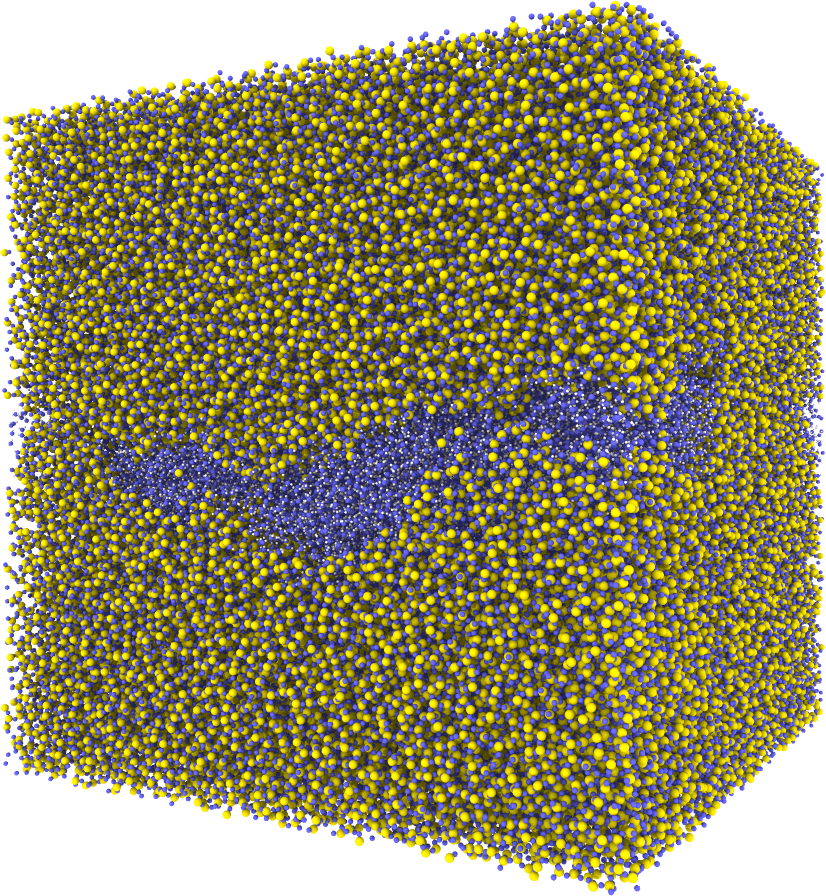
\includegraphics[width=\textwidth]{images/systems/trimmed-rough_fracture01_abel_13}%
        \caption{The whole system.}%
%         \label{fig:hex_to_tetra}%
    \end{subfigure}%
    \hfill%
        \begin{subfigure}[t]{\myfigwidth}%
        \centering% % Need to center to get image centered over caption
        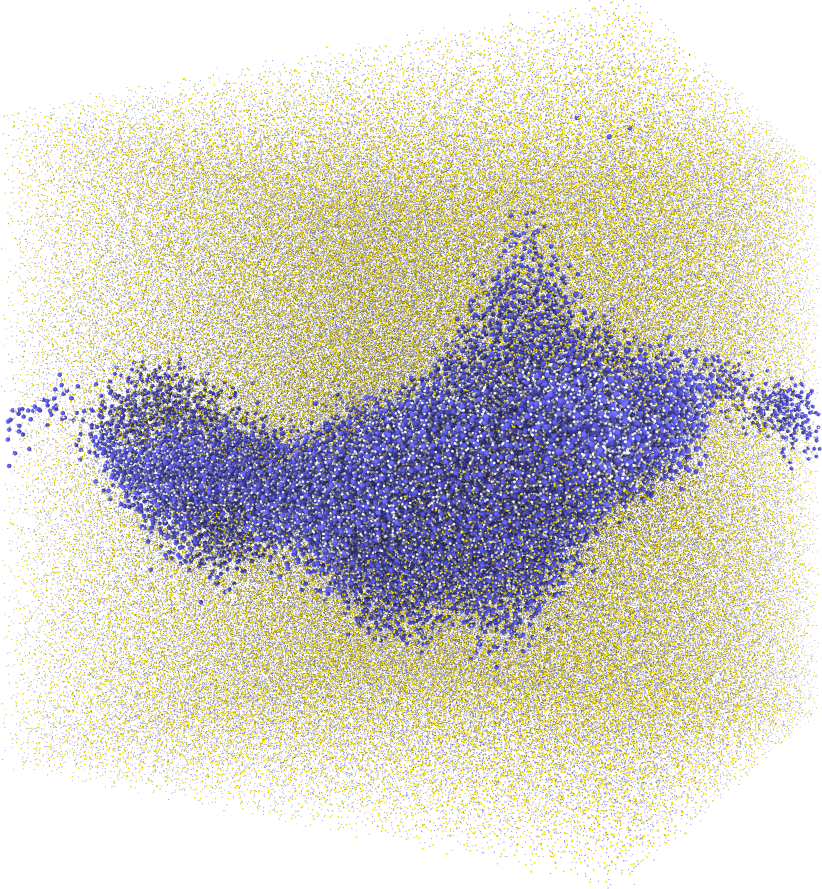
\includegraphics[width=\textwidth]{images/systems/trimmed-rough_fracture01_abel_15}%
        \caption{The whole system, with the size of the silicon and silica-oxygen atoms reduced to 0.1 \AA.}%
%         \label{fig:hex_to_tetra}%
    \end{subfigure}%
    \vspace{10pt}\\%
    \begin{subfigure}[t]{\myfigwidth}%
        \centering% % Need to center to get image centered over caption
        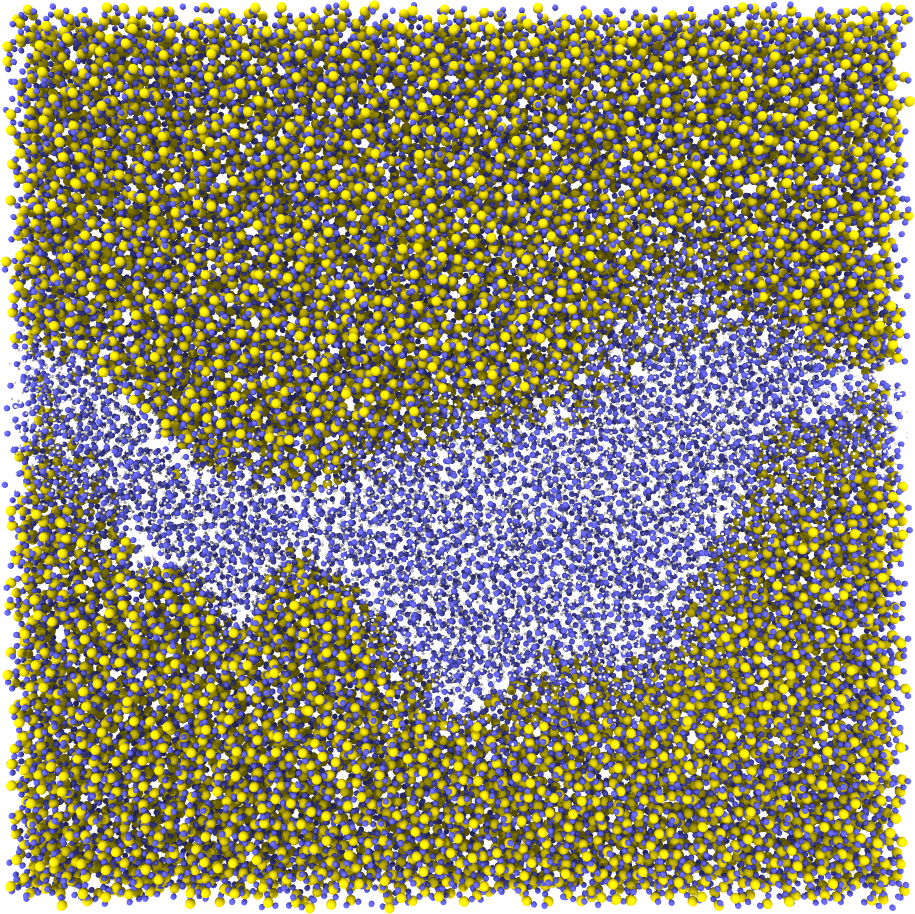
\includegraphics[width=\textwidth]{images/systems/trimmed-rough_fracture01_abel_16}%
        \caption{20 \AA\ thick slice.}%
%         \label{fig:hex_to_tetra}%
    \end{subfigure}%
    \hfill%
    %
    % ---- Rendering just water atoms ---- %
%     \begin{subfigure}[t]{\myfigwidth}%
%         \centering% % Need to center to get image centered over caption
%         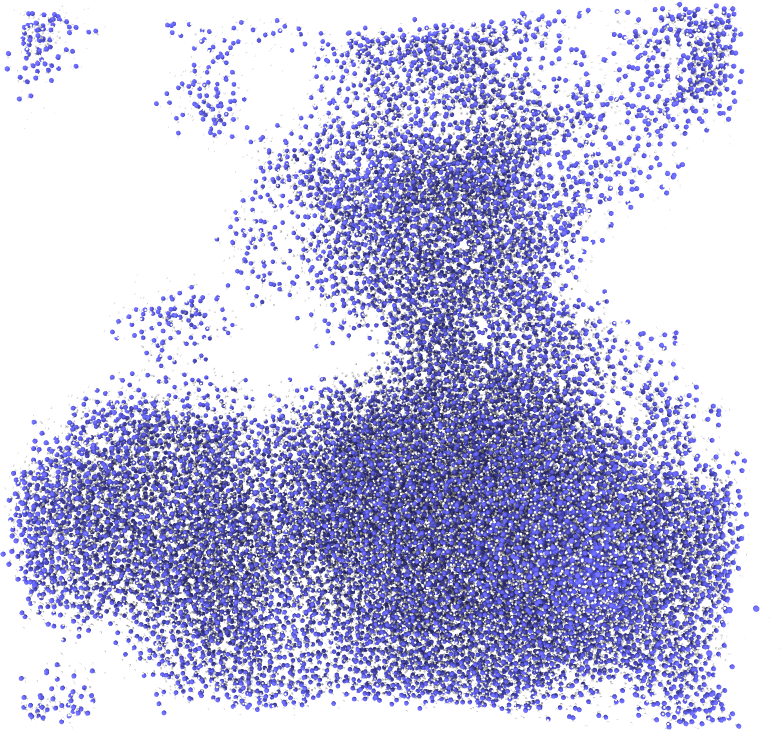
\includegraphics[width=\textwidth]{images/systems/trimmed-rough_fracture01_abel_17}%
%         \caption{Just the water molecules, viewed from above.}%
% %         \label{fig:hex_to_tetra}%
%     \end{subfigure}%
    % ----
    %
    % ---- Rendering of the water volume ---- %
    \begin{subfigure}[t]{\myfigwidth}%
        \centering% % Need to center to get image centered over caption
        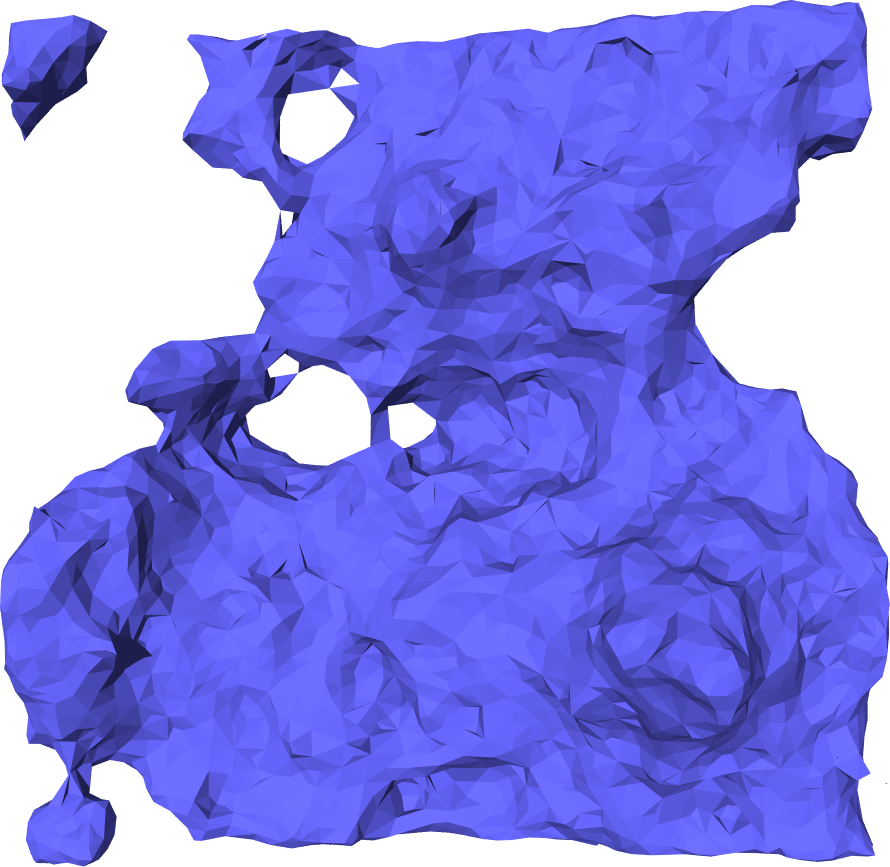
\includegraphics[width=\textwidth]{images/systems/trimmed-rough_fracture01_abel_22}%
        \caption{The pore volume.}%
%         \label{fig:hex_to_tetra}%
    \end{subfigure}%
    % ----
    \vspace{10pt}\\%
    \caption{%
        ``Rough fracture \#1'', a randomly generated fracture with varying width. \hl{Caption} %
        \label{fig:renderings_rough_fracture01_abel}%
    }%
\end{figure}%

%
\begin{figure}[!p]%
    \centering%
    \setlength{\myfigwidth}{0.55\textwidth}%
    \setlength{\myhfillwidth}{5mm}%
%     \setlength{\mycaptionwidth}{0.3\textwidth}%
%
% Use makebox to center figures below that are wider than \textwidth
%
\makebox[\textwidth][c]{%
    \begin{subfigure}[t]{\myfigwidth}%
        \centering% % Need to center to get image centered over caption
        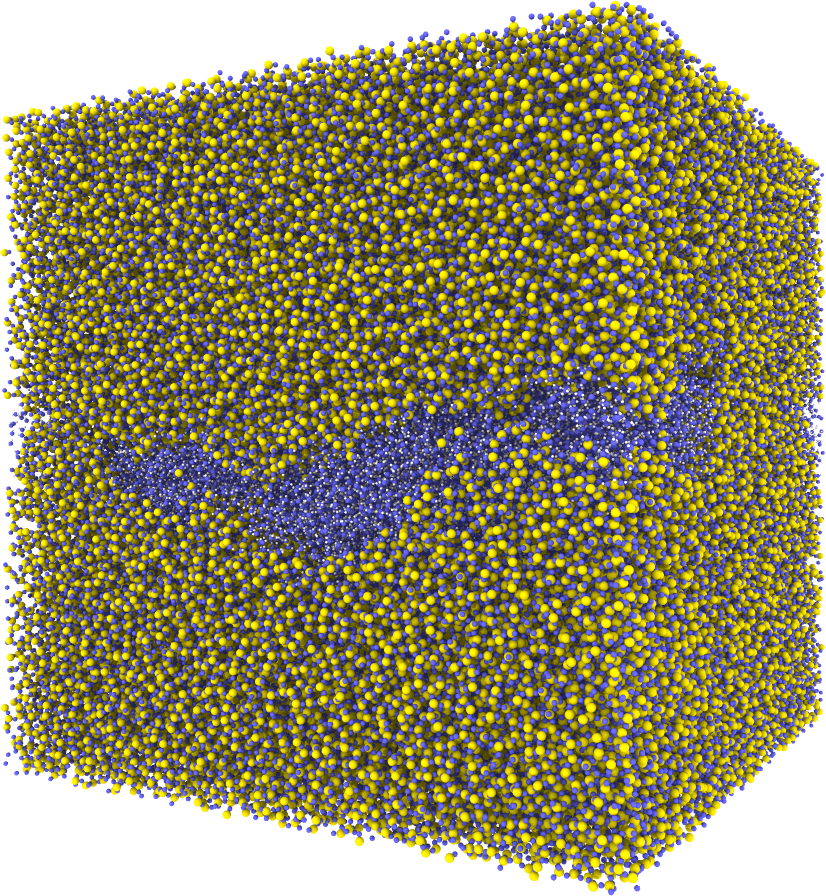
\includegraphics[width=\textwidth]{images/systems/trimmed-rough_fracture01_abel_13}%
        \caption{The whole system.}%
%         \label{fig:hex_to_tetra}%
    \end{subfigure}%
    %\hfill%
    \hspace{\myhfillwidth}%
        \begin{subfigure}[t]{\myfigwidth}%
        \centering% % Need to center to get image centered over caption
        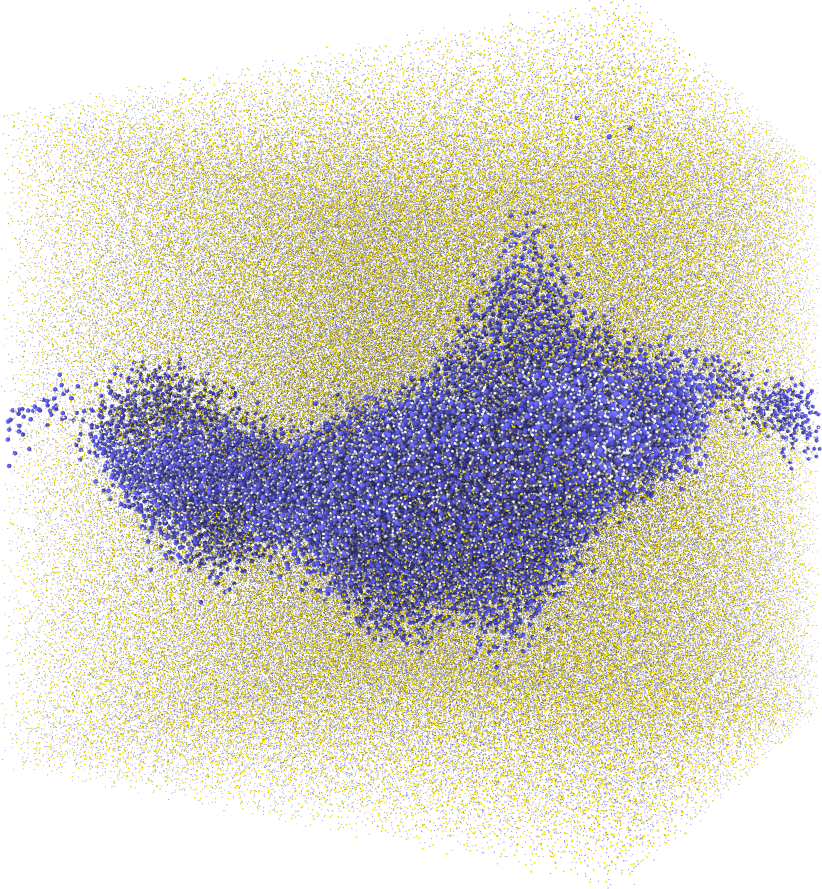
\includegraphics[width=\textwidth]{images/systems/trimmed-rough_fracture01_abel_15}%
        \caption{The whole system, with the size of the silicon and silica-oxygen atoms reduced to 0.1 \AA.}%
%         \label{fig:hex_to_tetra}%
    \end{subfigure}%
}%
    \vspace{10pt}\\%
\makebox[\textwidth][c]{%
    \begin{subfigure}[t]{\myfigwidth}%
        \centering% % Need to center to get image centered over caption
        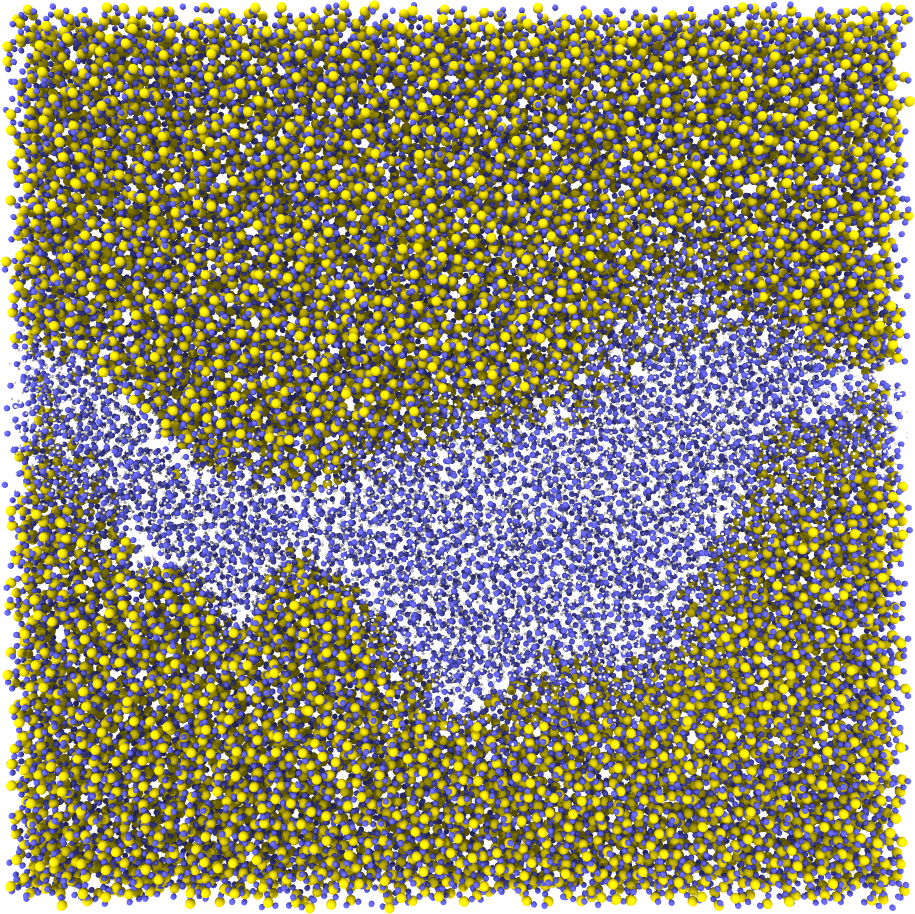
\includegraphics[width=\textwidth]{images/systems/trimmed-rough_fracture01_abel_16}%
        \caption{20 \AA\ thick slice.}%
%         \label{fig:hex_to_tetra}%
    \end{subfigure}%
%     \hfill%
    \hspace{\myhfillwidth}%
    %
    % ---- Rendering just water atoms ---- %
%     \begin{subfigure}[t]{\myfigwidth}%
%         \centering% % Need to center to get image centered over caption
%         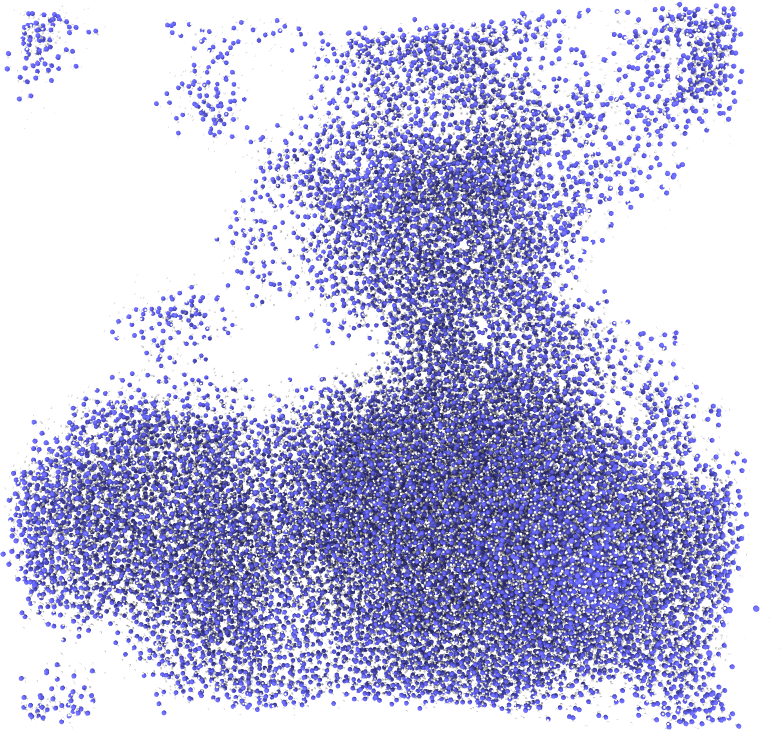
\includegraphics[width=\textwidth]{images/systems/trimmed-rough_fracture01_abel_17}%
%         \caption{Just the water molecules, viewed from above.}%
% %         \label{fig:hex_to_tetra}%
%     \end{subfigure}%
    % ----
    %
    % ---- Rendering of the water volume ---- %
    \begin{subfigure}[t]{\myfigwidth}%
        \centering% % Need to center to get image centered over caption
        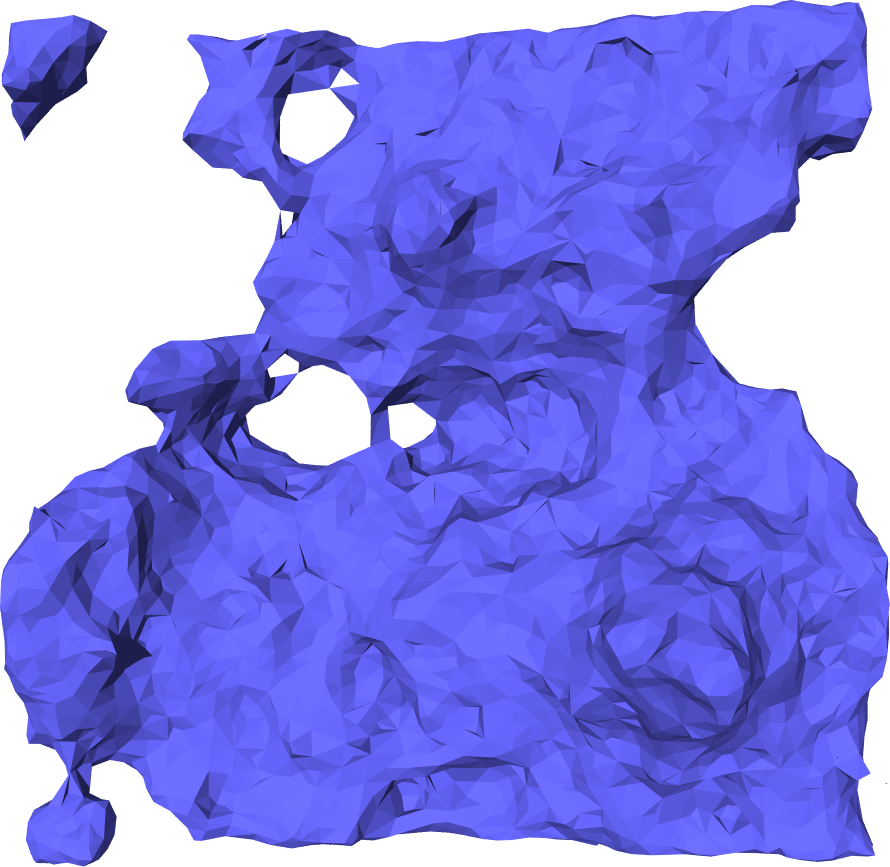
\includegraphics[width=\textwidth]{images/systems/trimmed-rough_fracture01_abel_22}%
        \caption{The pore volume.}%
%         \label{fig:hex_to_tetra}%
    \end{subfigure}%
    % ----
}%
    \vspace{10pt}\\%
    \caption{%
        ``Rough fracture \#1'', a randomly generated fracture with varying width. \hl{Caption} %
        \label{fig:renderings_rough_fracture01_abel}%
    }%
\end{figure}%

%
\begin{figure}[!p]%
    \centering%
    \setlength{\myfigwidth}{0.49\textwidth}%
%     \setlength{\mycaptionwidth}{0.3\textwidth}%
%
    \begin{subfigure}[t]{\myfigwidth}%
        \centering% % Need to center to get image centered over caption
        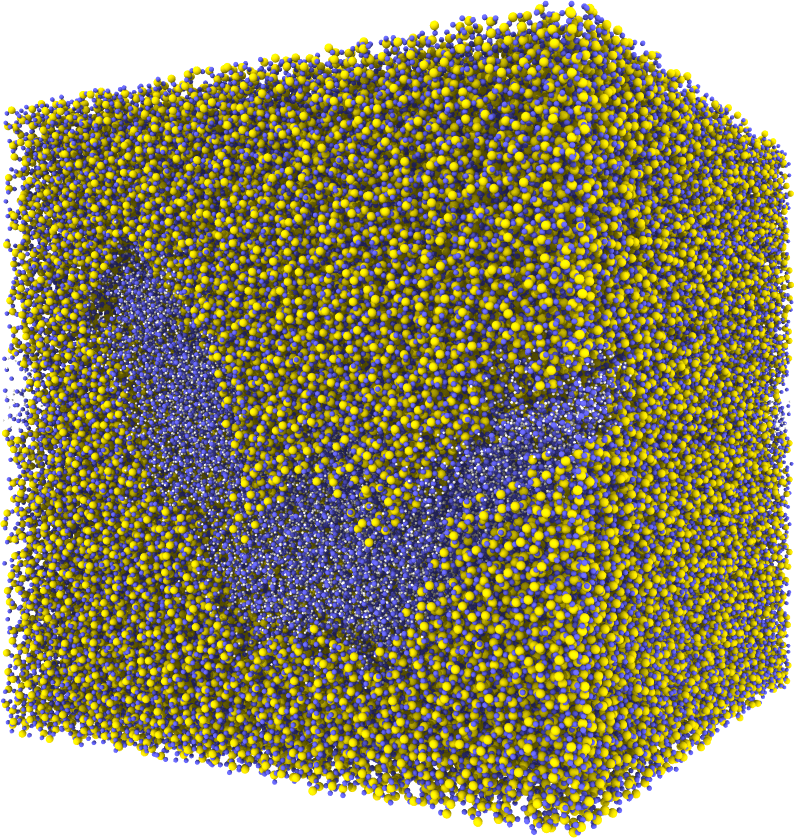
\includegraphics[width=\textwidth]{images/systems/trimmed-rough_fracture03_06}%
        \caption{The whole system.}%
%         \label{fig:hex_to_tetra}%
    \end{subfigure}%
    \hfill%
    \begin{subfigure}[t]{\myfigwidth}%
        \centering% % Need to center to get image centered over caption
        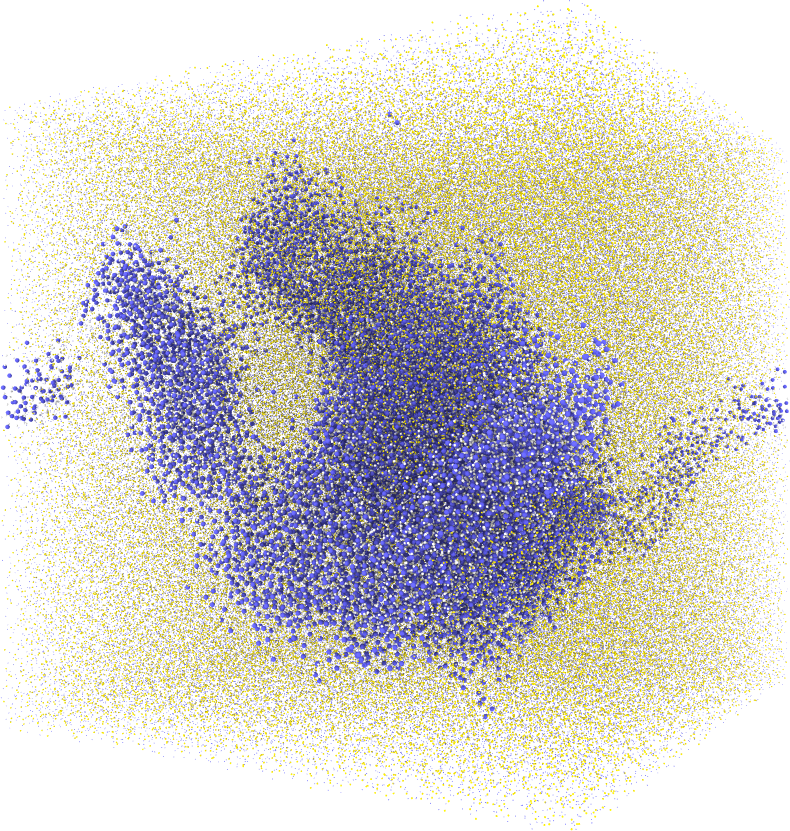
\includegraphics[width=\textwidth]{images/systems/trimmed-rough_fracture03_05}%
        \caption{The whole system, with the size of the silicon and silica-oxygen atoms reduced to 0.1 \AA.}%
%         \label{fig:hex_to_tetra}%
    \end{subfigure}%
    \vspace{10pt}\\%
    \begin{subfigure}[t]{\myfigwidth}%
        \centering% % Need to center to get image centered over caption
        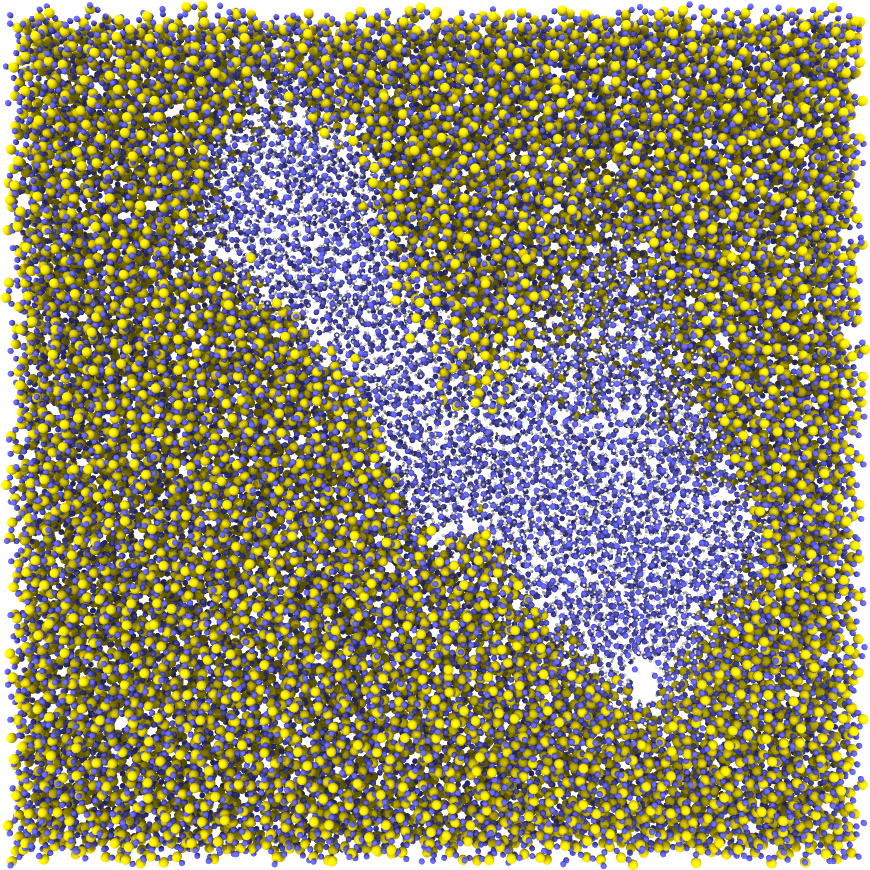
\includegraphics[width=\textwidth]{images/systems/trimmed-rough_fracture03_07}%
        \caption{20 \AA\ thick slice.}%
%         \label{fig:hex_to_tetra}%
    \end{subfigure}%
    \hfill%
    %
    % ---- Rendering just water atoms ---- %
%     \begin{subfigure}[t]{\myfigwidth}%
%         \centering% % Need to center to get image centered over caption
%         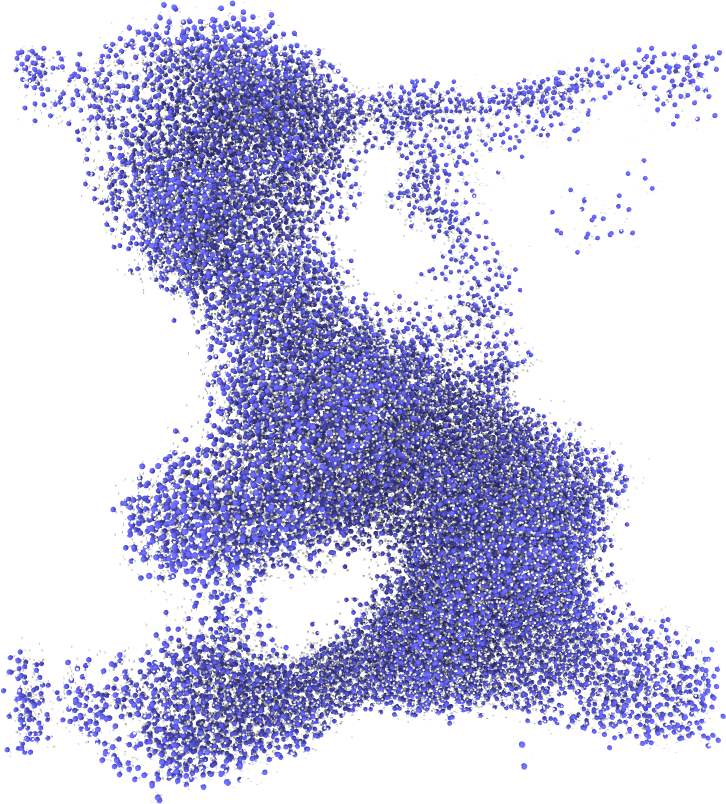
\includegraphics[width=\textwidth]{images/systems/trimmed-rough_fracture03_08}%
%         \caption{Caption.}%
% %         \label{fig:hex_to_tetra}%
%     \end{subfigure}%
    % ----
    %
    % ---- Rendering just water atoms ---- %
        \begin{subfigure}[t]{\myfigwidth}%
        \centering% % Need to center to get image centered over caption
        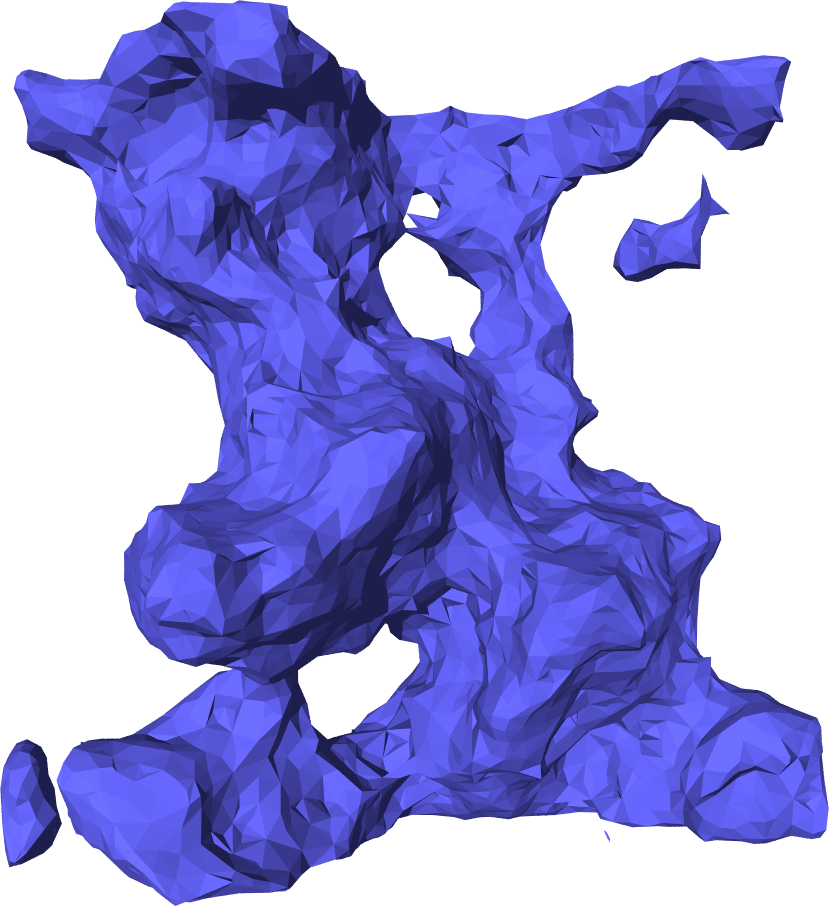
\includegraphics[width=\textwidth]{images/systems/trimmed-rough_fracture03_11}%
        \caption{The pore volume.}%
%         \label{fig:hex_to_tetra}%
    \end{subfigure}%
    % ----
    \vspace{10pt}\\%
    \caption{%
        ``Rough fracture \#2'', a randomly generated fracture with varying width. \hl{Caption} %
        \label{fig:renderings_rough_fracture03}%
    }%
\end{figure}%

%
\begin{figure}[!p]%
    \centering%
    \setlength{\myfigwidth}{0.49\textwidth}%
%     \setlength{\mycaptionwidth}{0.3\textwidth}%
%
    \begin{subfigure}[t]{\myfigwidth}%
        \centering% % Need to center to get image centered over caption
        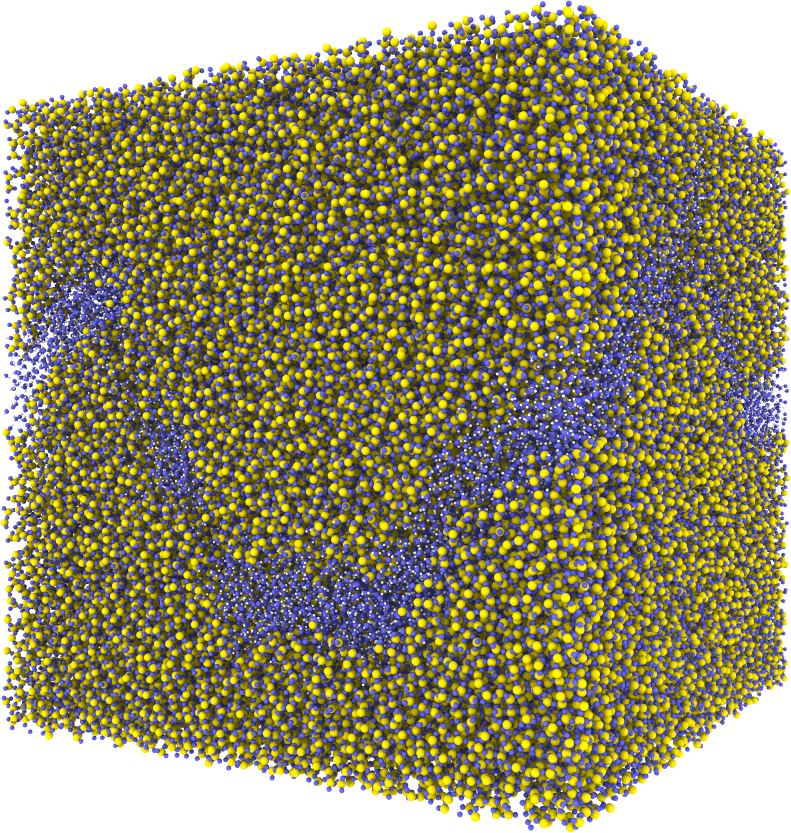
\includegraphics[width=\textwidth]{images/systems/trimmed-rough_fracture04_06}%
        \caption{The whole system.}%
%         \label{fig:hex_to_tetra}%
    \end{subfigure}%
    \hfill%
    \begin{subfigure}[t]{\myfigwidth}%
        \centering% % Need to center to get image centered over caption
        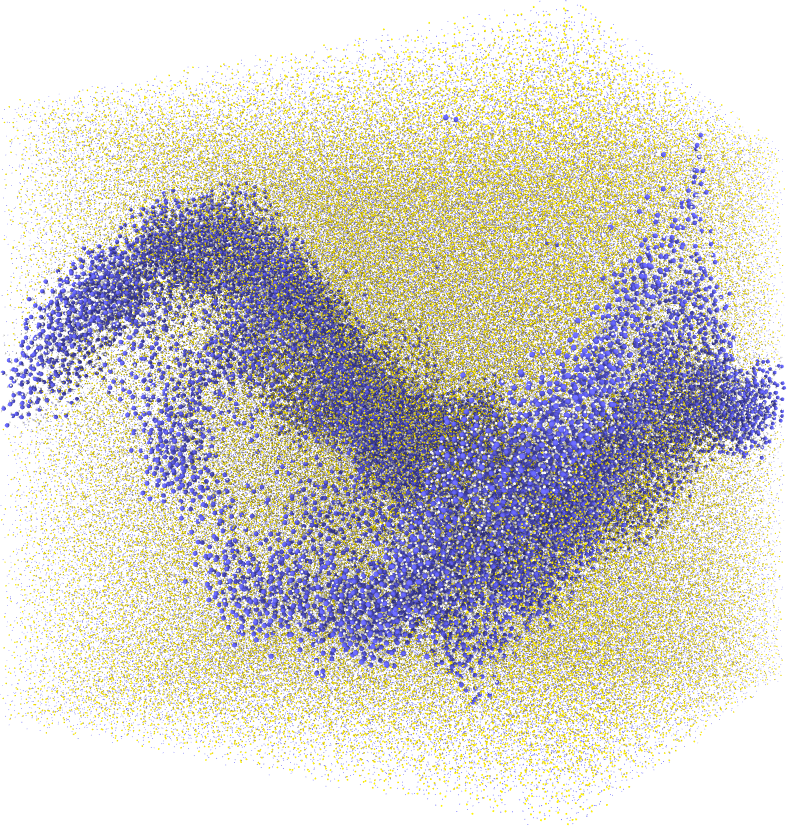
\includegraphics[width=\textwidth]{images/systems/trimmed-rough_fracture04_07}%
        \caption{The whole system, with the size of the silicon and silica-oxygen atoms reduced to 0.1 \AA.}%
%         \label{fig:hex_to_tetra}%
    \end{subfigure}%
    \vspace{10pt}\\%
    \begin{subfigure}[t]{\myfigwidth}%
        \centering% % Need to center to get image centered over caption
        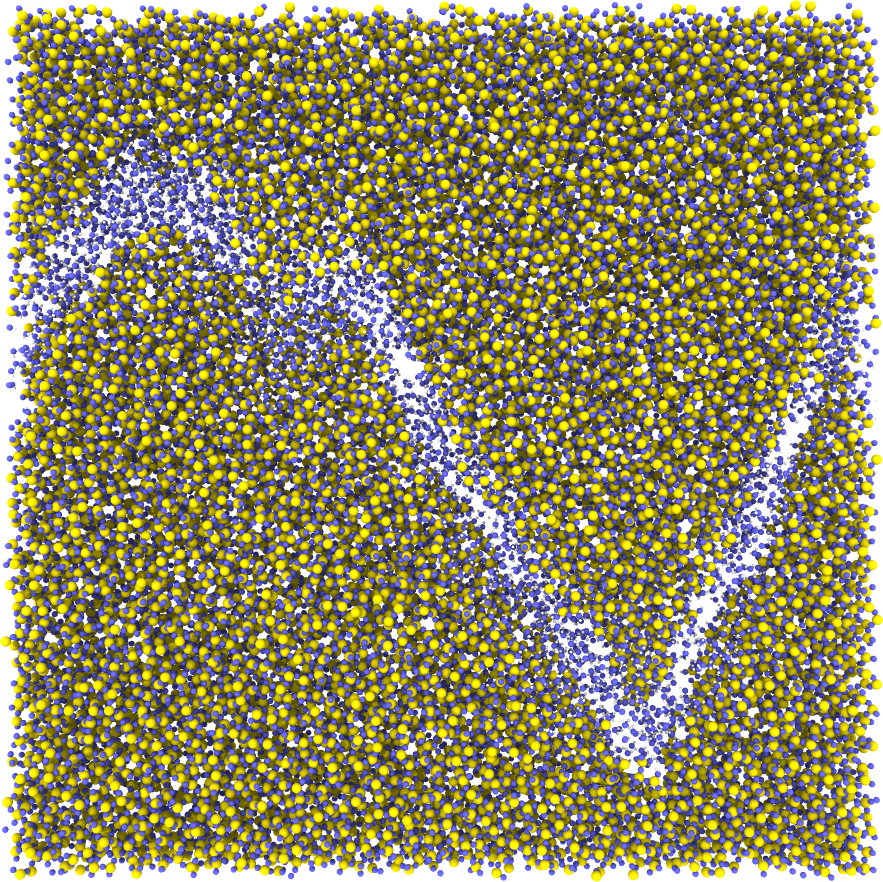
\includegraphics[width=\textwidth]{images/systems/trimmed-rough_fracture04_05_20ang}%
        \caption{20 \AA\ thick slice.}%
%         \label{fig:hex_to_tetra}%
    \end{subfigure}%
    \hfill%
    %
    % ---- Rendering just water atoms ---- %
%     \begin{subfigure}[t]{\myfigwidth}%
%         \centering% % Need to center to get image centered over caption
%         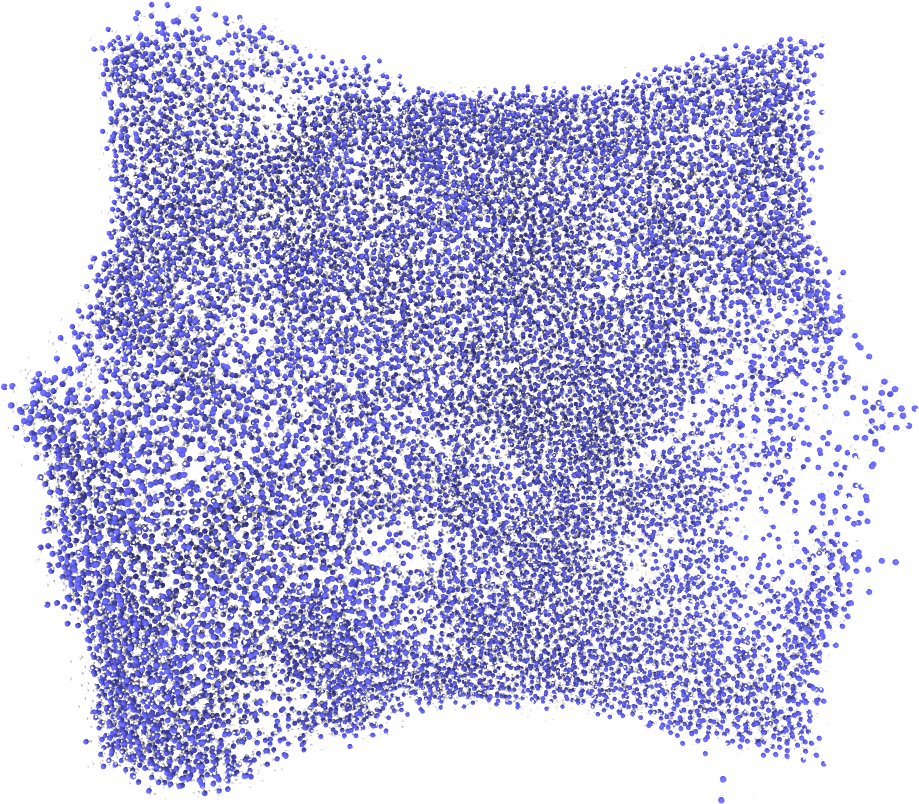
\includegraphics[width=\textwidth]{images/systems/trimmed-rough_fracture04_08}%
%         \caption{Caption.}%
% %         \label{fig:hex_to_tetra}%
%     \end{subfigure}%
    % ----
    %
    % ---- Rendering just water atoms ---- %
        \begin{subfigure}[t]{\myfigwidth}%
        \centering% % Need to center to get image centered over caption
        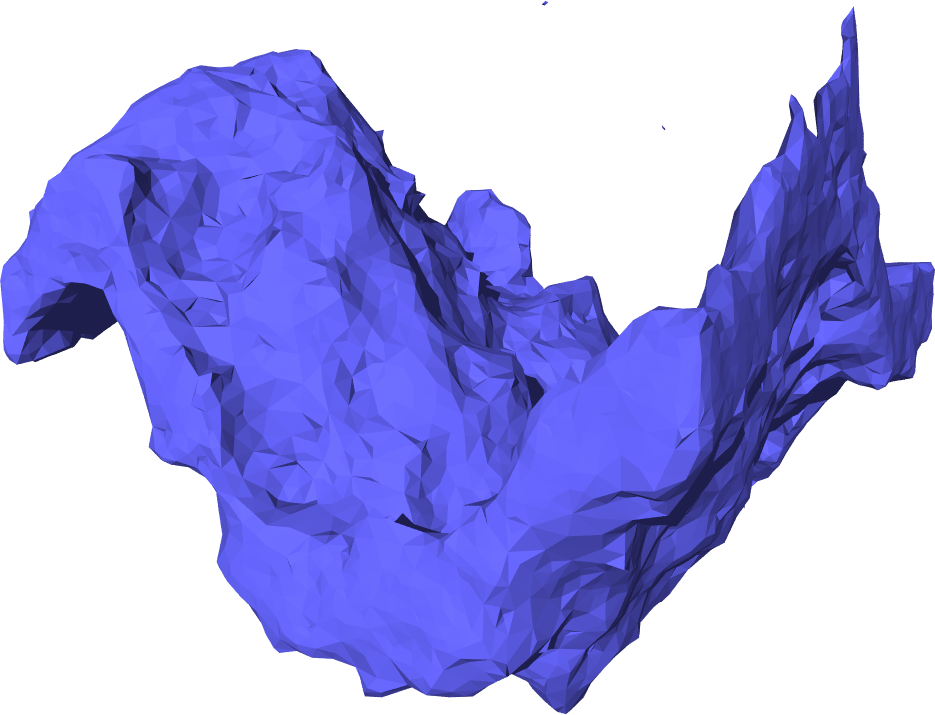
\includegraphics[width=\textwidth]{images/systems/trimmed-rough_fracture04_11}%
        \caption{The pore volume.}%
%         \label{fig:hex_to_tetra}%
    \end{subfigure}%
    % ----
    \vspace{10pt}\\%
    \caption{%
        ``Rough fracture \#3'', a randomly generated fracture generated from one surface repeated for the top and bottom half, with 14.4 \AA\ between the surfaces, giving approximately uniform width of the pore. \hl{Caption} %
        \label{fig:renderings_rough_fracture04_same_distance}%
    }%
\end{figure}%

%
\begin{figure}[!p]%
    \centering%
    \setlength{\myfigwidth}{0.49\textwidth}%
%     \setlength{\mycaptionwidth}{0.3\textwidth}%
%
    \begin{subfigure}[t]{\myfigwidth}%
        \centering% % Need to center to get image centered over caption
        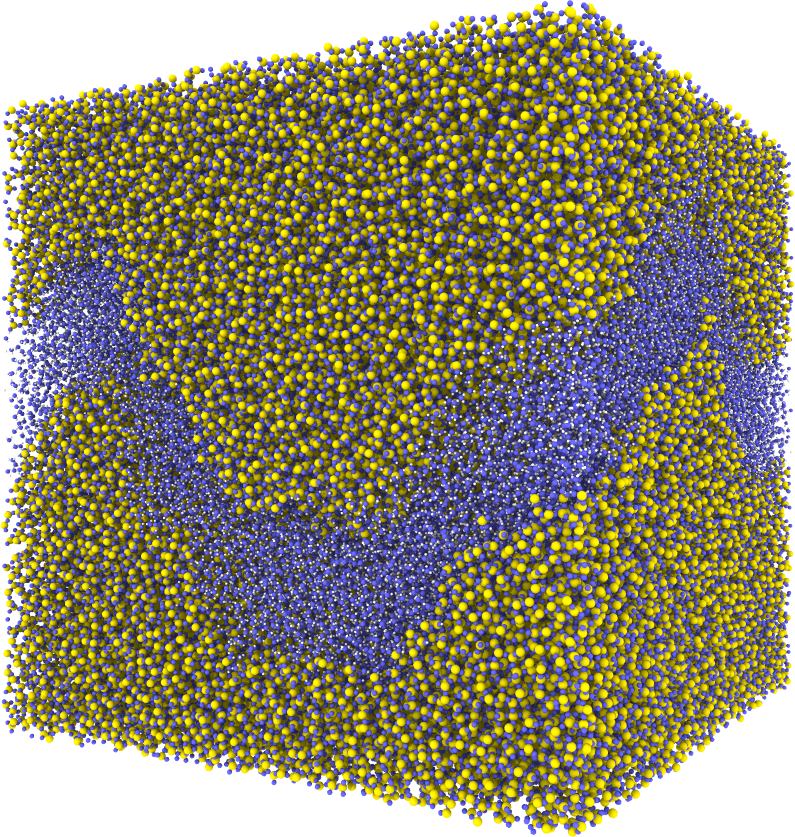
\includegraphics[width=\textwidth]{images/systems/trimmed-rough_fracture05_05}%
        \caption{The whole system.}%
%         \label{fig:hex_to_tetra}%
    \end{subfigure}%
    \hfill%
    \begin{subfigure}[t]{\myfigwidth}%
        \centering% % Need to center to get image centered over caption
        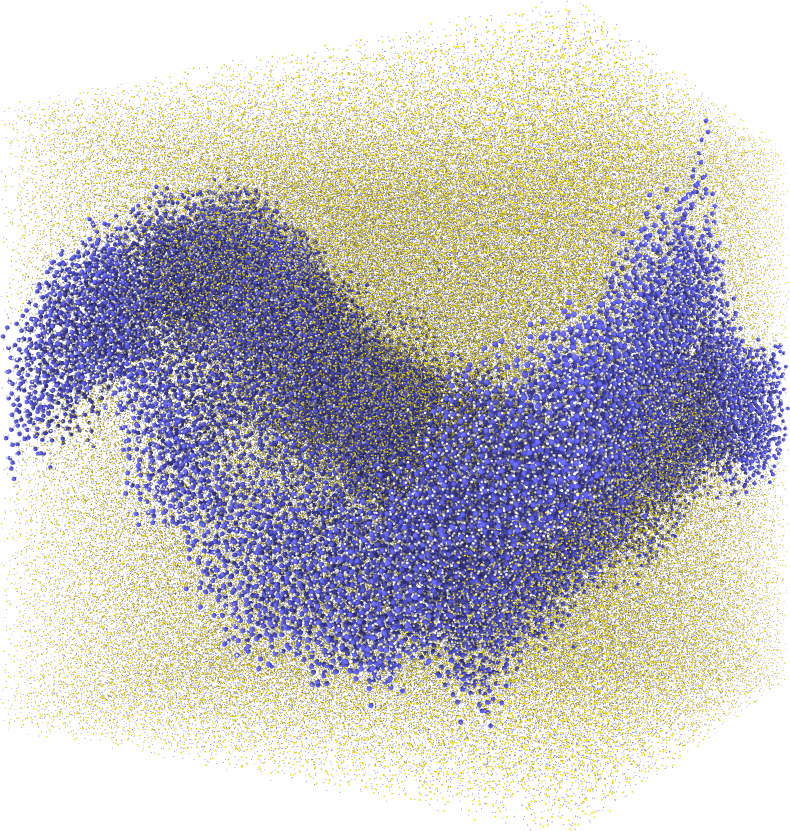
\includegraphics[width=\textwidth]{images/systems/trimmed-rough_fracture05_04}%
        \caption{The whole system, with the size of the silicon and silica-oxygen atoms reduced to 0.1 \AA.}%
%         \label{fig:hex_to_tetra}%
    \end{subfigure}%
    \vspace{10pt}\\%
    \begin{subfigure}[t]{\myfigwidth}%
        \centering% % Need to center to get image centered over caption
        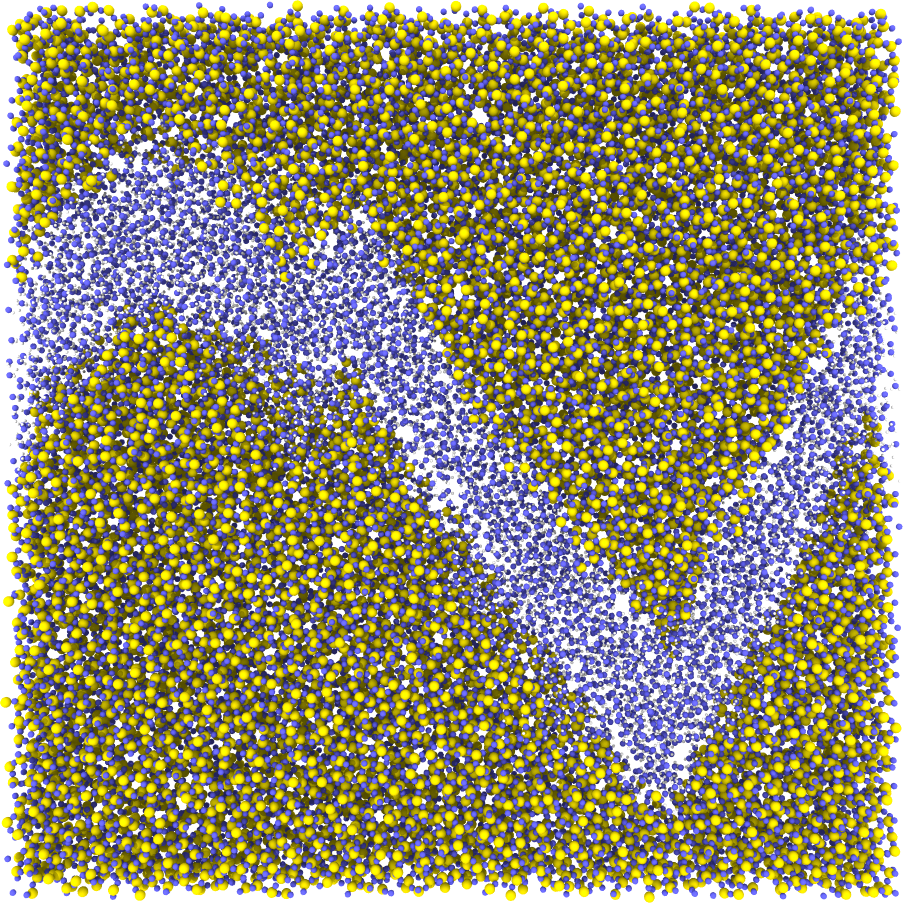
\includegraphics[width=\textwidth]{images/systems/trimmed-rough_fracture05_02_20ang}%
        \caption{20 \AA\ thick slice.}%
%         \label{fig:hex_to_tetra}%
    \end{subfigure}%
    \hfill%
    %
    % ---- Rendering just water atoms ---- %
%     \begin{subfigure}[t]{\myfigwidth}%
%         \centering% % Need to center to get image centered over caption
%         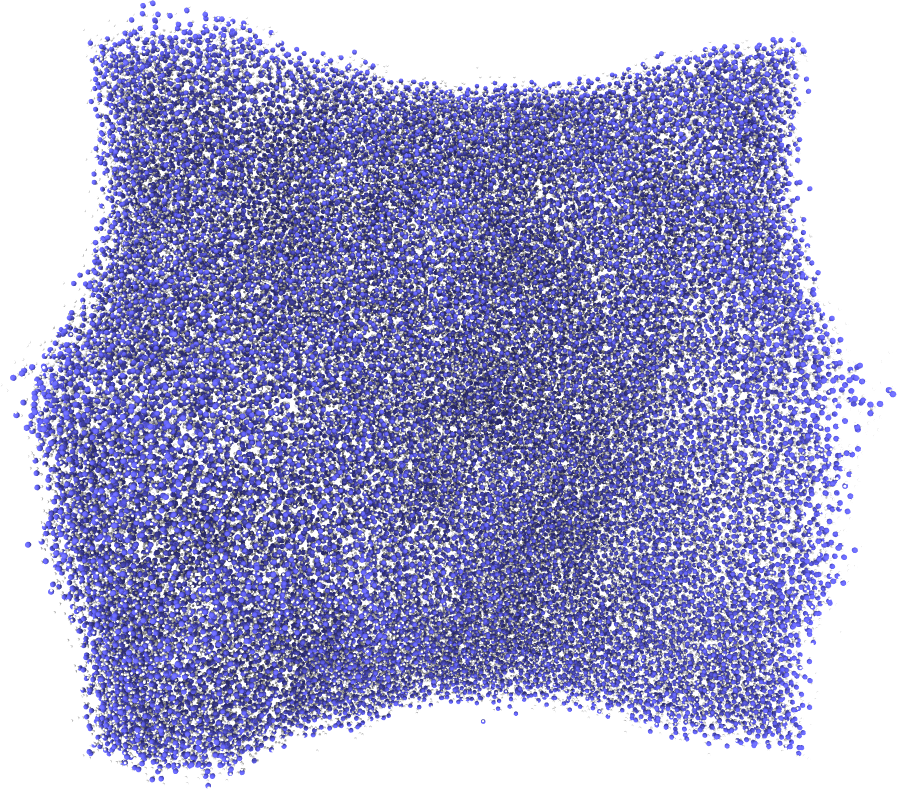
\includegraphics[width=\textwidth]{images/systems/trimmed-rough_fracture05_06}%
%         \caption{Caption.}%
% %         \label{fig:hex_to_tetra}%
%     \end{subfigure}%
    % ----
    %
    % ---- Rendering just water atoms ---- %
        \begin{subfigure}[t]{\myfigwidth}%
        \centering% % Need to center to get image centered over caption
        \includegraphics[width=\textwidth]{images/systems/trimmed-rough_fracture05_09}%
        \caption{The pore volume.}%
%         \label{fig:hex_to_tetra}%
    \end{subfigure}%
    % ----
    \vspace{10pt}\\%
    \caption{%
        ``Rough fracture \#4'', a randomly generated fracture generated from one surface repeated for the top and bottom half, with 28.8 \AA\ between the surfaces, giving approximately uniform width of the pore. \hl{Caption} %
        \label{fig:renderings_rough_fracture05}%
    }%
\end{figure}%

%
\begin{figure}[htpb]%
    \centering%
    \setlength{\myfigwidth}{0.49\textwidth}%
%     \setlength{\mycaptionwidth}{0.3\textwidth}%
%
    \begin{subfigure}[t]{\myfigwidth}%
        \centering% % Need to center to get image centered over caption
        \includegraphics[width=\textwidth]{images/systems/trimmed-flat_square_fracture02_03}%
        \caption{%
            ``Reference \#1'', a 86 \AA\ wide flat pore.  \hl{Caption} %
        }%
        \label{fig:renderings_flat_square_fracture02}%
    \end{subfigure}%
    \hfill%
    \begin{subfigure}[t]{\myfigwidth}%
        \centering% % Need to center to get image centered over caption
        \includegraphics[width=\textwidth]{images/systems/trimmed-flat_square_fracture03_04}%
        \caption{%
            ``Reference \#2'', a 86 \AA\ wide flat pore, with higher water density than \textbf{a)}. \hl{Caption} %
        }%
        \label{fig:renderings_flat_square_fracture03}%
    \end{subfigure}%
    \vspace{10pt}\\%
    \begin{subfigure}[t]{\myfigwidth}%
        \centering% % Need to center to get image centered over caption
        \includegraphics[width=\textwidth]{images/systems/trimmed-flat_fracture02_03}%
        \caption{%
            ``Reference \#3'', a 14.4 \AA\ wide flat pore. \hl{Caption} %
        }%
        \label{fig:renderings_flat_fracture02}%
    \end{subfigure}%
    \hfill%
    \begin{subfigure}[t]{\myfigwidth}%
        \centering% % Need to center to get image centered over caption
        \includegraphics[width=\textwidth]{images/systems/trimmed-flat_fracture03_03}%
        \caption{%
            ``Reference \#4'', a 28.8 \AA\ wide flat pore. \hl{Caption} %
        }%
        \label{fig:renderings_flat_fracture03}%
    \end{subfigure}%
    \vspace{10pt}\\%
    \caption{%
        Reference systems \#1-4.
        \label{fig:renderings_flat_fractures}%
    }%
\end{figure}%
%
        
    \chapter{Re}
\section{Density}
\begin{figure}[htpb]%
    \centering%
    \includesvg[width=0.7\textwidth, svgpath=./images/density/]{density_water02}%
    \caption{%
        Density of water. \hl{FINISH CAPTION}. %
%         \label{fig:cell_lists}%
    }%
\end{figure}%
\begin{figure}[htpb]%
    \centering%
    \includesvg[width=0.7\textwidth, svgpath=./images/density/]{number_of_molecules02}%
    \caption{%
        Number of molecules. Bin width = 0.2 \AA?. \hl{FINISH CAPTION}. %
%         \label{fig:cell_lists}%
    }%
\end{figure}%

\FloatBarrier
\section{Diffusion/mean square displacement}
\todo[inline]{Diffusion normal to and parallel to surface?}
\begin{figure}[htpb]%
    \centering%
    {
        \newcommand{\f}{\footnotesize}
        \includesvg[width=0.7\textwidth, svgpath=./images/diffusion/]{diffusion01}%
    }
    \caption{%
        Diffusion. \hl{FINISH CAPTION}. %
%         \label{fig:cell_lists}%
    }%
\end{figure}%

\begin{figure}[htpb]%
    \centering%
    {
        \newcommand{\f}{\footnotesize}%
        \includesvg[width=0.7\textwidth, svgpath=./images/diffusion/]{diffusion_constant02}%
    }
    \caption{%
        Diffusion. \hl{Consider fixing label background...} \hl{FINISH CAPTION}. %
%         \label{fig:cell_lists}%
    }%
\end{figure}%

\FloatBarrier
\section{Distance to atom}
\todo{replace these with results from actual fracture system?}
We developed a program that finds the distance to the nearest atom, in all points of the 
%
\setlength{\myfigwidth}{0.90\textwidth}%
\begin{figure}[htpb]%
    \centering%
    \includesvg[width=\myfigwidth, svgpath = ./images/distance_to_atom/]{SiO2_06_slice_r05_n256}%
    \caption{$r = 5$ \Ang}%
    \label{fig:distance_to_atom_r05}%
\end{figure}%
%
\begin{figure}[htpb]%
    \centering%
    \includesvg[width=\myfigwidth, svgpath = ./images/distance_to_atom/]{SiO2_06_slice_r20_n256}%
    \caption{$r = 20$ \Ang}%
    \label{fig:distance_to_atom_r20}%
\end{figure}%

\FloatBarrier
\section{``Generation matrix''}
\todo{replace these with results from actual fracture system?}
Not very useful. Much of the same as distance to atom, only worse (but faster).
%
\begin{figure}[htpb]%
    \centering%
    \includesvg[width=\myfigwidth, svgpath = ./images/generation_matrix/]{SiO2_06_slice_r05_n256}%
    \caption{5 generations}%
    \label{fig:generation_matrix_r05}%
\end{figure}%
%
\begin{figure}[htpb]%
    \centering%
    \includesvg[width=\myfigwidth, svgpath = ./images/generation_matrix/]{SiO2_06_slice_r11_n256}%
    \caption{11 generations}%
    \label{fig:generation_matrix_r11}%
\end{figure}%
%
\begin{figure}[htpb]%
    \centering%
    \includesvg[width=\myfigwidth, svgpath = ./images/generation_matrix/]{SiO2_06_slice_r40_n256}%
    \caption{40 generations}%
    \label{fig:generation_matrix_r40}%
\end{figure}%

\FloatBarrier
\section{Tetrahedral order parameter}


% \setlength{\myfigwidth}{0.499\textwidth}%
% \begin{figure}[htpb]%
%     \centering%
%     \begin{subfigure}[b]{\myfigwidth}%
%         \includesvg[width=\textwidth, svgpath=./images/tetrahedral_order_parameter/]{figure04}%
%         \caption{Caption}%
% %         \label{fig:pass_tet01}%
%     \end{subfigure}%
% %     \hspace{0.05\textwidth}%
%     \begin{subfigure}[b]{\myfigwidth}%
%         \includesvg[width=\textwidth, svgpath=./images/tetrahedral_order_parameter/]{figure07}%
%         \caption{Caption}%
% %         \label{fig:pass_tet02}%
%     \end{subfigure}%
%     
%     \begin{subfigure}[b]{\myfigwidth}%
%         \includesvg[width=\textwidth, svgpath=./images/tetrahedral_order_parameter/]{figure09}%
%         \caption{Caption}%
% %         \label{fig:pass_tet02}%
%     \end{subfigure}%
%     \begin{subfigure}[b]{\myfigwidth}%
%         \includesvg[width=\textwidth, svgpath=./images/tetrahedral_order_parameter/]{figure10}%
%         \caption{Caption}%
% %         \label{fig:pass_tet02}%
%     \end{subfigure}%
%     
%     \begin{subfigure}[b]{\myfigwidth}%
%         \includesvg[width=\textwidth, svgpath=./images/tetrahedral_order_parameter/]{figure11}%
%         \caption{Caption}%
% %         \label{fig:pass_tet02}%
%     \end{subfigure}%
%     \begin{subfigure}[b]{\myfigwidth}%
%         \includesvg[width=\textwidth, svgpath=./images/tetrahedral_order_parameter/]{figure12}%
%         \caption{Caption}%
% %         \label{fig:pass_tet02}%
%     \end{subfigure}%
%     %
%     \caption{%
%         \hl{Caption}%
%     }%
% %     \label{fig:inject_empty_voxel}%
% \end{figure}%

%
\begin{figure}[htpb]%
    \centering%
    \includesvg[width=1.0\textwidth, svgpath = ./images/tetrahedral_order_parameter/]{fancyfig04}%
    \caption{}%
%     \label{fig:distance_to_atom_r20}%
\end{figure}%

\FloatBarrier
\section{Area}
\section{Volume?}


        \section{Density of water\label{sec:results_density}}
% We measure the density as function of distance to the matrix in all our systems. We ended up with ``bulk'' densities in the systems ranging from around 1000 kg/m$^3$ to 1150 kg/m$^3$, so for easier comparison we have normalized the densities against the bulk density in each system. Here we have defined the bulk density as the average density of water molecules more than $\sim 10\text{ \AA}$ from the nearest silicon atom. 

We have measured the density of water as function of distance to the silica matrix in all of our systems, averaged over 200 states for each system, with 100 timesteps of 0.050 picoseconds between each state (5 picoseconds between each state). The results are plotted in \crefrange{fig:first_density_fig}{fig:last_density_fig}. We measured for distances ranging from 0 to 10 \AA\ from the silica matrix, in steps of 0.25 \AA. We have also measured the bulk density in the systems where this was possible, the results of which are listed in \cref{tab:bulk_water_density}. The plots start at 3.0 \AA, since water molecules closer to the silica matrix than this are most likely bound to silica atoms, and are part of the passivating silanol groups, as we saw in \cref{sec:distance_to_matrix_issues}.%
%
% ---- Subcaption/subfigure version ---- %
\begin{figure}[!htb]%
    % \centering%
    \setlength{\myfigwidth}{0.58\textwidth}%  % change "b" to "t" to anchor top instead of bottom
    \makebox[\textwidth][c]{ % to center figures below that are wider than \textwidth
        \begin{minipage}[t]{\myfigwidth}%
            \captionsetup[subfigure]{width=0.9\textwidth}%
            \centering%
            \includesvg[width=\textwidth, svgpath=./images/density/]{density_water04_reference}%
            \subcaption{%
                Dashed lines are (red, \#3) 14.4 \AA\ and (teal, \#4) 28.8 \AA\ narrow flat pores, solid lines are 86 \AA\ wide flat pores.%
                \label{fig:density_reference_systems}%
            }%
        \end{minipage}%
        \hfill%
        \begin{minipage}[t]{\myfigwidth}%
            \captionsetup[subfigure]{width=0.9\textwidth}%
            \centering%
            \includesvg[width=\textwidth, svgpath=./images/density/]{density_water04_rough}%
            \subcaption{%
                Dashed lines are (red, \#3) 14.4 \AA\ and (teal, \#4) 28.8 \AA\ narrow fractures, solid lines are random fractures.%
                \label{fig:density_rough_systems}%
            }%
        \end{minipage}%
    }%
    \vspace{8pt}%
    \caption{%
        Water density ($\rho$) as function of distance to silica matrix ($r$) in \textbf{(a)} all four reference systems (flat pores) and \textbf{(b)} rough fracture systems.%
        %In \textbf{(a)} the dashed lines are 14.4 (red dashed line, \#3) and 28.8 (teal dashed line, \#4) \AA\ narrow flat pores \textbf{a)} flat pores and \textbf{b)} narrow, uniform width fractures. \hl{FINISH CAPTION}.%
        \label{fig:first_density_fig}%
    }%
\end{figure}%

The most significant trend we notice in \cref{fig:first_density_fig} is that the water density seems stable at 9-10 \AA\ from the silica matrix, but as we move closer than this we see a clear reduction in density. When we go from 10 \AA\ and move closer to the matrix we see in all systems that the density falls off at around 7-8 \AA\, and is reduced by almost 10\% at around 5 \AA. The density then increases to densities higher than the initial densities (the ones at 10 \AA) when we move towards 3 \AA. The relative reduction and then increase in density seems to be similar in all systems with similar overall densities, but in the systems with the highest overall density the relative change seems to be a bit smaller than in the other systems.

We now look at the density in the four reference systems, which is plotted in \cref{fig:density_reference_systems}. We see that the densities all have the same quantitative behaviour as we move further from the silica matrix, even though the net density is very different in the four systems, with the densities stabilizing at values ranging from 1050 to almost 1150 kg/m$^3$ at 8-10 \AA. One trend we notice is that the point where the density stabilizes, at around 7 \AA, seems to appear closer to the matrix when we increase the overall density. The minimum point seems to appear at approximately the same distance for the systems with a 86 \AA\ wide flat pore (system \#1 and \#2), but a bit closer to the matrix for the narrow flat pores (system \#4 and \#3).

In \cref{fig:density_rough_systems} we have plotted the density in the four random fracture systems. We see that the density in all four systems are very similar at all distances to the matrix, and that the density seems to stabilize between 1010 and 1025 kg/m$^3$ at 8-10 \AA\ from the silica matrix. We see that even though these four fractures have different geometries (especially system \#1 and \#2 are very different from system \#3 and \#4), the behaviour of the density as we go from 8 to 3 \AA\ from the silica matrix seems to be the same in all four systems. We also see that the density seems peak at around 8 \AA, and stabilize at a somewhat lower value as we go further from the silica matrix. This peak is similar to a peak observed around 5 \AA\ from the silica matrix by Bonnaud et al. in \cite{bonnaud2010molecular} (see Figure 6 in the article). In the article they use a different measure for the distance to the silica matrix, which might explain the difference in the distance at which the peak is observed.

We have estimated the bulk water density by the same technique we use for measuring water density as function of distance to the silica matrix, but now by averaging the density for all water-oxygen atoms further away from the silica matrix than a certain distance (typically 10 \AA\ or more), instead of using bins. This measurement requires that we have a fracture at least twice as wide as this distance to have any atoms we can measure the density of, so estimating the bulk density was only possible in reference system \#1 and \#2 with a flat, constant fracture of 86 \AA, and in the two random fractured systems \#1 and \#2, which have fractures with varying width. %We measured the bulk distance using a minimum distance to the matrix of 10 and 30 \AA\, to see if there was a difference between these two limits.%
%
\begin{table}[!htb]%
    \centering%
    \begin{tabular}{l|cc|cc}%
    ~               & \multicolumn{2}{c|}{$r>10$ \AA}& \multicolumn{2}{c}{$r>30$ \AA}    \\
    \textit{System} & Density [kg/m$^3$]    & N     & Density [kg/m$^3$]    & N   \\ \hline
    Reference \#1   & 1038.4                & 49k   & 1038.5                & 20k \\
    Reference \#2   & 1092.7                & 52k   & 1090.4                & 21k \\
    Rough \#1       & 1017.9                & 5.0k  & -                     & 0   \\
    Rough \#2       & 1002.8                & 4.2k  & -                     & 0   \\
    \end{tabular}%
    \vspace{8pt}%
    \caption{%
        Estimated bulk water densities, and the number of water molecules used in the calculations. Estimated using Voronoi tesselation, averaged over voronoi volumes for all water-oxygen atoms further away from silica matrix than 10 and 30 \AA\ (hydrogen atoms were removed before Voronoi tesselation). %
        \label{tab:bulk_water_density}%
    }%
\end{table}%
% bulk density (r>10.0) rough_fracture01_abel = 1018
% bulk density (r>10.0) rough_fracture03 = 1003
% bulk density (r>10.0) flat_square_02 = 1038
% bulk density (r>10.0) flat_square_03 = 1094

The estimated bulk densities are listed in \cref{tab:bulk_water_density}, where we have measured the bulk density for water atoms at least 10 \AA\ and at least 30 \AA\ from the silica matrix. We see that the estimated bulk density does not change if we use 10 or 30 \AA\ as the minimum distance from the matrix, indicating that a limit of 10 \AA\ is probably safe. If we compare the bulk densities to the plots of the density as function of distance from the matrix in \cref{fig:density_reference_systems,fig:density_rough_systems}, we see that the density seems to be stable close to the bulk density at around 10 \AA.

In \cref{fig:density_all} we have plotted the density in all eight systems we have simulated. For easier comparisons we have also tried normalizing the density against an estimated bulk density, plotted in \cref{fig:density_all_normalized}. In both figures we see the same trend as before, where the falloff for the density seems to move closer to the matrix as we increase the overall density. We see a hint of a similar trend for the minimum point of the density, but not nearly as clear as for the falloff point. We also notice that the falloff seems to be closer to the silica matrix for the rough fracture systems than for the flat pores, with the falloff being near 8 \AA\ in the rough fracture systems, but from 7 to 8 \AA\ for the flat pores, depending on the density.
\todoa{More about these two figures}
%
\begin{figure}[!p]%
    \centering%
    \setlength{\myfigwidth}{0.88\textwidth}%
    \setlength{\mycaptionwidth}{0.09999\textwidth}%
    %
    \begin{minipage}[c]{\myfigwidth}%
%         \includesvg[width=\textwidth, svgpath=./images/density/]{density_water04_all}%
        \includesvg[width=\textwidth, svgpath=./images/density/]{density_water04_all_trends}%
    \end{minipage}%
    \begin{minipage}[c]{\mycaptionwidth}%
        \subcaption{\label{fig:density_all}}%
    \end{minipage}%
    \\%
    \begin{minipage}[c]{\myfigwidth}%
        \includesvg[width=\textwidth, svgpath=./images/density/]{density_water04_all_normalized_divide}%
    \end{minipage}%
    \begin{minipage}[c]{\mycaptionwidth}%
        \subcaption{\label{fig:density_all_normalized}}%
    \end{minipage}%
    %
    \captionsetup{width=\textwidth}% since it's a floatpage figure
    \caption{%
        Density of water in all systems, as function of distance from the silica matrix. Dashed lines are reference systems, and solid lines rough fracture systems. In \textbf{(b)} the density has been normalized against the approximate bulk density, estimated from the density at 10 \AA\ from the silica matrix. %
        \label{fig:last_density_fig}%
    }%
\end{figure}%

\subsubsection*{Injection density vs. actual density}
To check the accuracy of the method we use for filling the fractures and pores with water, we want to compare the input densities used when filling the pores to the actual resulting density in the systems. We have already found the bulk density in four of the systems, but in the other systems we are not able to measure the density in the same way. What we do in these systems (``rough fracture'' \#3 and \#4, and reference system \#3 and \#4) is to approximate the bulk density by looking at the value of the density near 10 \AA\ from the silica matrix. This should give us a somewhat useable approximation to the bulk density in the system\footnote{In rough fracture system \#3 and reference system \#3 we do not have any measurements for water molecules around 10 \AA\ from the matrix, since these systems have pores that are narrower than 20 \AA. For these systems we extrapolate the the density at 10 \AA\ from the values we have.}.

The results can be seen in \cref{tab:estimate_bulk_density}. We see that using the value at 10 \AA\ gives a good approximation to the measured bulk density for the system where we are able to measure the bulk density, and that the method for filling the fractures and pores with water performs well when the pores and fracures are very large. But we also see that in the systems with very narrow pores, the method for filling the pore with water seems to struggle with acheving the wanted density. This is cause by the voxelation method we use when finding room for water molecules, as expected and noted previously.
%
\begin{table}[!htb]%
    \centering%
    \begin{tabular}{l|ccc}%
    \textit{System} & Input $D$ [kg/m$^3$]  & Measured $D$ [kg/m$^3$]   & Approx. $D$ at 10 \AA \\ \hline
    Reference \#1   & 1050                  & 1038                      & 1045 \\
    Reference \#2   & 1126                  & 1093                      & 1098 \\
    Reference \#3   & 1273                  & -                         & 1085 \\
    Reference \#4   & 1273                  & -                         & 1135 \\
    Rough \#1       & 1050                  & 1018                      & 1022 \\
    Rough \#2       & 1050                  & 1003                      & 1010 \\
    Rough \#3       & 1273                  & -                         & 1025 \\
    Rough \#4       & 1273                  & -                         & 1016 \\
    \end{tabular}%
    \vspace{8pt}%
    \caption{%
        A comparison of the estimated and measured bulk water density in the systems we have simulated, with the input density we used when filling the fractures with water.
        \label{tab:estimate_bulk_density}%
    }%
\end{table}%
        \FloatBarrier
        \section{Diffusion/mean square displacement}
\todod{Diffusion normal to and parallel to surface?}
\todob{Plot of $r^2$ for 200 and 40 states to argue for origo move?}

% bulk diff in Ref \#1 = 0.202034846318
%   N = mean(47577, 47524, 47555, 47552, 47559) = 
% bulk diff in Ref \#2 = 0.178684448075
%   N = mean(50280, 50284, 50291, 50275, 50321)

% bulk diff in Rough \#1 = 0.197721045372      
%   N = mean(4271, 4279, 4252, 4294, 4284)
% bulk diff in Rough \#2 = 0.208658027239  
%   N = mean(3414, 3396, 3419, 3431, 3393)


To produce these results we have averaged over 200 states, with 100 timesteps of 20.67 md units between each timestep ($\sim 0.5$ picoseconds\hl{???}), divided into 5 non-overlapping origos, with 40 states per origo.

We first look at the diffusion as function of distance to the silica matrix in the four reference systems, which we have plotted in \cref{fig:diffusion_reference_systems}. We see that the diffusion constant, $D$, has similar quantitative behaviour as we move further from the silica matrix in all four reference systems, but that the actual $D$ is different in each system. The two systems with 86 \AA\ wide flat pores have diffusion constants that differ by around 10-30\%, even though those two systems should be pretty similar. The main difference between those two systems is the density, as we saw in \cref{sec:results_density}. We have listed the bulk $D$ in \cref{tab:bulk_water_diffusion}, and we see that the bulk diffusion for the two reference systems with 86 \AA\ wide flat pores is {0.202 \AA$^2$/ps}, while system \#2 has {0.179 \AA$^2$/ps}, with a difference of {13 \%}. \hl{So it seems like the increased density in reference system \#2 have had an impact on the diffusion -- so we use ref \#1 when comparing to other systems?}
%
%
% \begin{figure}[htpb]%
%     \centering%
%     \includesvg[width=0.6\textwidth, svgpath=./images/diffusion/]{diffusion_constant_move_origin_reference01}%
%     \caption{%
%         Diffusion constant as function of distance to silica matrix for all four reference systems (flat fractures). The solid lines are for the two systems with 86 \AA\ wide fractures, and the dashed lines for narrow fractures of 14.4 and 28.8 \AA. \hl{FINISH CAPTION}. %
%         \label{fig:diffusion_reference_systems}%
%     }%
% \end{figure}%

In \cref{fig:diffusion_rough_systems} we have plotted the diffusion constant %as function of distance from the silica matrix 
for the four random fracture systems, ``rough \#1'' through 4. We again see a quantitative similar behaviour, and we see that all systems except the 14.4 \AA\ narrow fracture (``rough \#3'') have very similar diffusion constants and behaviour. In \cref{tab:bulk_water_diffusion} see that the bulk diffusion constants in the two regular random fractures (\#1 and \#2) are similar, with a difference of {6 \%}. We also see that the $D$ for water at 7-10 \AA\ from the silica matrix is close to the bulk constant for these two systems.
\todoao{More about diffusion?}
%
% \begin{figure}[htpb]%
%     \centering%
%     \includesvg[width=0.6\textwidth, svgpath=./images/diffusion/]{diffusion_constant_move_origin_rough01}%
%     \caption{%
%         Diffusion constant as function of distance to silica matrix for all four random/rough fractures. \hl{FINISH CAPTION}. %
%         \label{fig:diffusion_rough_systems}%
%     }%
% \end{figure}%
%
%
% ---- Minipage ---- %
% \begin{figure}[htpb]%
% % \centering%
% \setlength{\myfigwidth}{0.58\textwidth}%
% \makebox[\textwidth][c]{ % to center figures below that are wider than \textwidth
%     \begin{minipage}[t]{\myfigwidth}%
%         \captionsetup{width=0.925\textwidth}%
%         \centering%
%         \includesvg[width=\textwidth, svgpath=./images/diffusion/]{diffusion_constant_move_origin_reference01}%
%         \caption{%
%             Diffusion constant ($D$) as function of distance to silica matrix ($r$) for all four reference systems (flat pores). The solid lines are the two systems with 86 \AA\ wide pores, and the dashed lines are 14.4 and 28.8 \AA\ narrow flat pores. \hl{FINISH CAPTION}. %
%             \label{fig:diffusion_reference_systems}%
%         }%
%     \end{minipage}%
%     \hfill%
%     \begin{minipage}[t]{\myfigwidth}% % change "b" to "t" to anchor top instead of bottom
%         \captionsetup{width=0.925\textwidth}% % minipage defines a \textwidth for it's own, so we have to repeat this command inside the minipage
%         \centering%
%         \includesvg[width=\textwidth, svgpath=./images/diffusion/]{diffusion_constant_move_origin_rough01}%
%         \caption{%
%             Diffusion constant ($D$) as function of distance to silica matrix ($r$) for all four random rough fractures. Solid lines are regular random fractures, and dashed lines are narrow fractures with uniform width of 14.4 and 28.8 \AA. \hl{FINISH CAPTION}. %
%             \label{fig:diffusion_rough_systems}%
%         }%
%     \end{minipage}%
% }
% \end{figure}%
%
% ---- Subcaption ---- %
\begin{figure}[htpb]%
% \centering%
\setlength{\myfigwidth}{0.58\textwidth}%
\makebox[\textwidth][c]{ % to center figures below that are wider than \textwidth
    \begin{minipage}[t]{\myfigwidth}%
        \centering%
        \includesvg[width=\textwidth, svgpath=./images/diffusion/]{diffusion_constant_move_origin_reference01}%
        \subcaption{\label{fig:diffusion_reference_systems}}%
    \end{minipage}%
    \hfill%
    \begin{minipage}[t]{\myfigwidth}% % change "b" to "t" to anchor top instead of bottom
        \centering%
        \includesvg[width=\textwidth, svgpath=./images/diffusion/]{diffusion_constant_move_origin_rough01}%
        \subcaption{\label{fig:diffusion_rough_systems}}%
    \end{minipage}%
}%
\caption{%
    Diffusion constant ($D$) as function of distance from silica matrix ($r$), for \textbf{a)} all reference systems and \textbf{b)} all rough fractures. Dashed lines are 14.4 and 28.8 \AA\ \textbf{a)} flat pores and \textbf{b)} narrow, uniform width fractures. \hl{FINISH CAPTION}. %
}%
\end{figure}%

% \begin{figure}[htpb]%
%     \centering%
%     {
%         \newcommand{\f}{\footnotesize}
%         \includesvg[width=0.7\textwidth, svgpath=./images/diffusion/]{diffusion01}%
%     }
%     \caption{%
%         Diffusion. \hl{Make new figure using new diffusion program}. %
% %         \label{fig:cell_lists}%
%     }%
% \end{figure}%

% \begin{figure}[htpb]%
%     \centering%
%     {
%         \newcommand{\f}{\footnotesize}%
%         \includesvg[width=0.7\textwidth, svgpath=./images/diffusion/]{diffusion_constant02}%
%     }
%     \caption{%
%         Diffusion. \hl{Make new figure using new diffusion program} \hl{FINISH CAPTION}. %
% %         \label{fig:cell_lists}%
%     }%
% \end{figure}%

The bulk diffusion constants have been estimated in the two reference systems with 86 \AA\ wide flat pores (reference \#1 and \#2), and in rough system \#1 and \#2, by measuring $D$ for all water molecules further away from the silica matrix than 10 \AA. The results can be seen in \cref{tab:bulk_water_diffusion}. The other four systems have very narrow pores and fractures, with most of the water molecules closer to the silica matrix than 10 \AA\, so we haven't measured the bulk diffusion in those systems, and we don't expect much of the water to have bulk behaviour\todobo{explain this better?}.
%
\begin{table}[!htb]%
    \centering%
    \begin{tabular}{l|cc}%
        \textit{System} & Bulk $D$ [\AA$^2$/ps] & N    \\\hline
        Reference \#1   & 0.202                 & 48k  \\ % 0.202034846318
        Reference \#2   & 0.179                 & 50k  \\ % 0.178684448075
        Rough \#1       & 0.198                 & 4.3k \\ % 0.197721045372
        Rough \#2       & 0.209                 & 3.4k \\ % 0.208658027239
    \end{tabular}%
    \vspace{8pt}%
    \caption{%
        Bulk diffusion constant for water (for $r>10$ \AA), and the number of water molecules used in the calculations. %
        \label{tab:bulk_water_diffusion}%
    }%
\end{table}

In \cref{fig:diffusion_normal_and_reference} we have plotted diffusion for the two normal random fractures (with varying pore width) together with all four reference systems. We see that the behaviour of $D$ as function of the distance to the silica matrix in the two fracture systems is very similar to each other, and matches the behaviour in reference system \#1 pretty well. This reference system is the one with a 86 \AA\ wide flat pore and the lowest bulk density of the two reference systems with wide flat pores ($\rho \approx 1038$ kg/m$^3$ compared to $\approx 1091$ kg/m$^3$).
\todoa{Write something about rough vs. reference and uniform rough vs. narrow flat pore figures below.}%

In \cref{fig:diffusion_narrow_and_reference} we have plotted the diffusion for the two random narrow fractures with uniform width together with all four reference systems. We see that the diffusion in the 14.4 \AA\ narrow fracture (``Rough \#3'') almost exactly matches the the diffusion in the reference system with a 14.4 \AA\ flat pore (``Ref \#4''). We also see that the 28.8 \AA\ narrow fracture (``Rough \#4'') has higher diffusion than the flat reference system with a 28.8 \AA\ flat pore (``Ref \#4''), but that it matches the reference system with a 86 \AA\ flat pore (``Ref \#1'') very well\todobo{discuss this?}.
%
% ---- Minipage version ---- %
% \begin{figure}[htpb]%
% % \centering%
% \setlength{\myfigwidth}{0.58\textwidth}%
% \makebox[\textwidth][c]{ % to center figures below that are wider than \textwidth
%     \begin{minipage}[t]{\myfigwidth}%
%         \captionsetup{width=0.925\textwidth}%
%         \centering%
%         \includesvg[width=\textwidth, svgpath=./images/diffusion/]{diffusion_constant_move_origin_normal01}%
%         \caption{%
%             Diffusion constant ($D$) as function of distance from silica matrix ($r$), for random rough fractures and all reference systems. \hl{reference figure or remove} \hl{FINISH CAPTION}. %
%             \label{fig:diffusion_normal_and_reference}%
%         }%
%     \end{minipage}%
%     \hfill%
%     \begin{minipage}[t]{\myfigwidth}% % change "b" to "t" to anchor top instead of bottom
%         \captionsetup{width=0.925\textwidth}% % minipage defines a \textwidth for it's own, so we have to repeat this command inside the minipage
%         \centering%
%         \includesvg[width=\textwidth, svgpath=./images/diffusion/]{diffusion_constant_move_origin_narrow01}%
%         \caption{%
%             Diffusion constant ($D$) as function of distance from silica matrix ($r$), for random narrow fractures and all reference systems. \hl{reference figure or remove} \hl{FINISH CAPTION}. %
%             \label{fig:diffusion_narrow_and_reference}%
%         }%
%     \end{minipage}%
% }
% \end{figure}%
%
% ---- Subcaption/subfigure version ---- %
\begin{figure}[htpb]%
% \centering%
\setlength{\myfigwidth}{0.58\textwidth}%
\makebox[\textwidth][c]{ % to center figures below that are wider than \textwidth
    \begin{minipage}[t]{\myfigwidth}%
        \centering%
        \includesvg[width=\textwidth, svgpath=./images/diffusion/]{diffusion_constant_move_origin_normal01}%
        \subcaption{\label{fig:diffusion_normal_and_reference}}%
    \end{minipage}%
    \hfill%
    \begin{minipage}[t]{\myfigwidth}% % change "b" to "t" to anchor top instead of bottom
        \centering%
        \includesvg[width=\textwidth, svgpath=./images/diffusion/]{diffusion_constant_move_origin_narrow01}%
        \subcaption{\label{fig:diffusion_narrow_and_reference}}%
    \end{minipage}%
}%
\caption{%
    Diffusion constant ($D$) as function of distance from silica matrix ($r$), for \textbf{a)} rough fracture system \#1 and \#2 (normal rough fractures) and all reference systems, and \textbf{b)} the narrow uniform width fractures (fracture system \#3 and \#4) and all reference systems. Dashed lines are reference systems. %
}%
\end{figure}%

% \begin{figure}[htpb]%
%     \centering%
%     \includesvg[width=0.8\textwidth, svgpath=./images/diffusion/]{diffusion_constant_move_origin_normal01}%
%     \caption{%
%         Diffusion for random rough fractures and reference systems. \hl{reference figure or remove} \hl{FINISH CAPTION}. %
% %         \label{fig:cell_lists}%
%     }%
% \end{figure}%
% 
% \begin{figure}[htpb]%
%     \centering%
%     \includesvg[width=0.8\textwidth, svgpath=./images/diffusion/]{diffusion_constant_move_origin_narrow01}%
%     \caption{%
%         Diffusion for random narrow fractures and reference systems. \hl{reference figure or remove} \hl{FINISH CAPTION}. %
% %         \label{fig:cell_lists}%
%     }%
% \end{figure}%

% \begin{figure}[htpb]%
%     \centering%
%     \includegraphics[width=0.5\textwidth]{images/diffusion/mean_square_displacement_interesting.png}%
%     \caption{%
%         Something interesting (msd stops increasing for a couple of angstrom near 4.5-5, 5-5.5, 5.5-6.0) \hl{reference figure or remove} \hl{FINISH CAPTION}. %
% %         \label{fig:cell_lists}%
%     }%
% \end{figure}%

% \begin{figure}[htpb]%
%     \centering%
%     \setlength{\myfigwidth}{0.49\textwidth}%
% %     \setlength{\mycaptionwidth}{0.3\textwidth}%
% %
%     \begin{subfigure}[b]{\myfigwidth}%
%         \includesvg[width=\textwidth, svgpath=./images/diffusion/]{diffusion_constant_move_origin01}%
%         \caption{%
%             Diffusion. \hl{FINISH CAPTION}. %
%     %         \label{fig:cell_lists}%
%         }%
%     \end{subfigure}%
%     \hfill%
%     \begin{subfigure}[b]{\myfigwidth}%
%         \includesvg[width=\textwidth, svgpath=./images/diffusion/]{diffusion_constant_move_origin02}%
%         \caption{%
%             Diffusion. \hl{FINISH CAPTION}. %
%     %         \label{fig:cell_lists}%
%         }%
%     \end{subfigure}%
%     \caption{%
%         rough\_fracture\_01\_abel - ``Rough fracture \#1'' \hl{Caption} %
%         \label{fig:renderings_rough_fracture01_abel}%
%     }%
% \end{figure}%
        \FloatBarrier
        \section{Tetrahedral order parameter}
% \todoa{Bin width 0.5 \AA\ and $\Delta Q = 0.01$ for all results! ($\Delta Q$ isn't shown anywhere)}
% \todoa{Make two separate TOP figures, one for regular rough, and one for rough with same surfac x2 ?}
% \todoa{Update bulk TOP figure with results from long analysis run}
% %
% \begin{figure}[htpb]%
%     \centering%
%     \includesvg[width=1.0\textwidth, svgpath = ./images/tetrahedral_order_parameter/]{fancyfig04}%
%     \caption{}%
% %     \label{fig:distance_to_atom_r20}%
% \end{figure}%
%
% \begin{figure}[htpb]%
%     \centering%
%     \includesvg[%
% %         width=\textwidth,% choose which fits best, width or height (regular includegraphics can use both and add "keepaspectratio", but includesvg can't)
%         height=\textheight,%
%         svgpath = ./images/tetrahedral_order_parameter_new/]{figure01}%
%     \caption{\hl{Caption, add legends!}}%
% %     \label{fig:distance_to_atom_r20}%
% \end{figure}%
%

We have measured the thetrahedral order parameter for our four reference systems, and the four random fracture systems, and plotted the \hl{relative occurrence/probability} $P(Q)$ as function of $Q$, for water molecules with different distances from the silica matrix. We used used 150 bins for the $Q$-values, with $\Delta Q = 0.01$, and bins of $\Delta r = 0.5$ for the different distances to the matrix, for all measurements presented here. The results are plotted in \crefrange{fig:first_top_figure}{fig:last_top_figure}. We have also measured the bulk order parameter, which is plotted in \cref{fig:top_bulk}.

For comparison we have also estimated $P(Q)$ in bulk water, by measuring the tetrahedral order parameter for all water molecules further from the silica matrix than 10 \AA, in the two reference systems with 86 \AA\ wide flat pores. The results for bulk water can be seen in \cref{fig:top_bulk}. We see that we get \hl{two peaks (``bimodal''?)}, one just above $Q = 0.5$ and one right below $Q = 0.75$. \todoao{Compare with some reference, for example Mathilde's ref [26]?}
%
\begin{figure}[htpb]%
    \centering% 
    \includesvg[%
        width=0.5\textwidth,
        svgpath = ./images/tetrahedral_order_parameter_new/%
    ]{figure01_bulk}%
    \caption{%
        Plot of tetrahedral order parameter for bulk water (water molecules further than 10 \AA\ from the silica matrix), in the two reference systems with 86 \AA\ wide flat pores (reference system \#1 and \#2, see \cref{fig:renderings_flat_square_fracture02,fig:renderings_flat_square_fracture03}). The average $Q$ is indicated by a vertical line. %
    }%
    \label{fig:top_bulk}%
\end{figure}%

In \cref{fig:top_normal_and_reference,fig:top_narrow01_and_reference,fig:top_narrow02_and_reference} we have plotted the results for different combinations of random fractures and flat pores. We have plotted this for a total of %
% 10 %
8 %
different distances from the silica matrix, for $Q$-values ranging from -0.5 to 1.0. 

We see that all systems have pretty similar behaviour for different $Q$-values, but we also see that $P(Q)$ changes a lot when we go from 3.0 \AA\ from the silica matrix to 5 \AA. At 5.5 \AA we are already pretty close to the bulk behaviour seen in \cref{fig:top_bulk}, with a small gradual change from 5.5 \AA\ to 6.5 \AA\ (and further to 10 \AA, not plotted here), where we are close to bulk behaviour. In general we see that near the silica matrix water seems to have a very different internal coordination compared to in bulk water, with the average $Q$-value going from $Q_\text{mean} \approx 0.2$ at $r = 3.0$ \AA\ to $Q_\text{mean} \approx 0.55$ at $r = 4.5$ \AA, in all systems, which is close to the bulk value of $Q_\text{mean, bulk} \approx 0.63$. We also see that the distribution has a different shape at $r = 4.5$ \AA\ than the bulk distribution. We also see that $P(Q)$ is much more spread out close to the silica matrix compared to further away, and that we only have a single peak, while bulk water has \hl{two peaks (``bimodal''?)} and is less spread out.\todobo{come up with something more accurate than ``spread out''}
\todob{Table of mean Q? Stddv?}

%
\begin{figure}[!p]%
    \centering%
    \includesvg[%
        width=\textwidth,% choose which fits best, width or height (regular includegraphics can use both and add "keepaspectratio", but includesvg can't)
%         height=\textheight,%
        svgpath = ./images/tetrahedral_order_parameter_new/%
    ]{figure02_regular_and_wide}%
    {%
        \captionsetup{width=\textwidth}%
        \caption{%
            Plot of $P(Q)$ for the two regular rough fractures (the solid lines), and a reference system with a 86 \AA\ wide flat pore (the dashed line) (see \cref{fig:renderings_rough_fracture01_abel,fig:renderings_rough_fracture03,fig:renderings_flat_square_fracture03}), for different distances to the silica matrix (as indicated by the text in top left corner of each plot). The average $Q$ is indicated by a vertical line. %
            \label{fig:top_normal_and_reference}%
            \label{fig:first_top_figure}%
        }%
    }%
\end{figure}%

In figure \cref{fig:top_normal_and_reference} we have plots of $P(Q)$ for rough systems \#1 and \#2, which are the two random rough fractures, and reference system \#1, which is a 86 \AA\ wide flat pore with a bulk water density of $\sim 1038$ kg/m$^3$. We see that the two random fracture systems have very similar behaviour, as expected, since they were prepared very similarly. We see that the average $Q$-value of the fracture systems is generally lower than in the reference system, and that the fracture systems seem to ``lag behind'' the reference system when we increase the distance to the silica matrix, with the fractured systems catching up the reference system near 6.5 \AA, as all three plots get close to a bulk-like shape.

%
\begin{figure}[!p]%
    \centering% 
    \includesvg[%
        width=\textwidth,% choose which fits best, width or height (regular includegraphics can use both and add "keepaspectratio", but includesvg can't)
%         height=\textheight,%
        svgpath = ./images/tetrahedral_order_parameter_new/%
    ]{figure02_flat_and_wide01}%
    {%
        \captionsetup{width=\textwidth}%
        \caption{%
            Plot of $P(Q)$ for a rough fracture with uniform width of 14.4 \AA\ (the blue solid line), a reference system with a 14.4 \AA\ wide flat pore (the dashed line), and a flat reference system with a 86 \AA\ wide flat pore (the red solid line) (see \cref{fig:renderings_rough_fracture04_same_distance,fig:renderings_flat_fracture03,fig:renderings_flat_square_fracture03}), for different distances to the silica matrix (as indicated by the text in top left corner of each plot). The average $Q$ is indicated by a vertical line. %
            \label{fig:top_narrow01_and_reference}%
        }%
    }%
\end{figure}%

In \cref{fig:top_narrow01_and_reference} we have plots of $P(Q)$ for rough system \#3, which is the fracture with uniform width of 14.4 \AA, and reference systems \#1 and \#3, which are the 86 and 14.4 \AA\ wide flat pores. %
We see that that the reference system with a wide flat pore seems to lie between the two systems with narrow pores for $r\in[3.5,5.5]$, and that the narrow fracture seems to lag behind the two reference systems as we increase $r$ from 3.5 to 6.0 \AA, with the behaviour in all systems being close to bulk at $6.0$ \AA. We see that the average $Q$ for the narrow fracture seems to lie lower than the wide flat pore reference system, and the narrow flat pore reference system seems to lie higher.
% We see the same trend in $P(Q)$ as before, with the average $Q$ being lower for the fracture and the narrow flat pore for $r < 5.5$ \AA, and the shape of $P(Q)$ getting close to bulk as $r\rightarrow 6.0$ \AA. We see that $P(Q)$ for the narrow flat pore seems to lie between the narrow fracture and the reference system, and that both the narrow fracture and narrow pore seems to lag behind the reference system as we increase the distance to the silic matrix.

%
\begin{figure}[!p]%
    \centering% 
    \includesvg[%
        width=\textwidth,% choose which fits best, width or height (regular includegraphics can use both and add "keepaspectratio", but includesvg can't)
%         height=\textheight,%
        svgpath = ./images/tetrahedral_order_parameter_new/%
    ]{figure02_flat_and_wide02}%
    {%
        \captionsetup{width=\textwidth}%
        \caption{%
            Plot of $P(Q)$ for a rough fracture with uniform width of 28.8 \AA\ (the blue solid line), a reference system with a 28.8 \AA\ wide flat pore (the dashed line), and a reference system with a 86 \AA\ wide flat pore (the red solid line) (see \cref{fig:renderings_rough_fracture05,fig:renderings_flat_fracture03,fig:renderings_flat_square_fracture03}), for different distances to the silica matrix (as indicated by the text in top left corner of each plot). The average $Q$ is indicated by a vertical line. %
            \label{fig:top_narrow02_and_reference}%
        }%
    }%
\end{figure}%

In \cref{fig:top_narrow01_and_reference} we have plots of $P(Q)$ for rough system \#4, which is the fracture with uniform width of 28.8 \AA, and reference systems \#1 and \#4, which are the 86 and 28.8 \AA\ wide flat pores. We see the same behaviour as for the 14.4 \AA\ fracture, albeit with the 28.8 \AA\ reference system being a bit closer to the reference system with a wide fracture.

In both \cref{fig:top_narrow01_and_reference,fig:top_narrow02_and_reference} it seems like the systems with a narrow flat pore (the red solid lines) seems to deviate the most from the wide reference system.

%
\begin{figure}[htpb]%
    \centering% 
    \includesvg[%
        width=\textwidth,% choose which fits best, width or height (regular includegraphics can use both and add "keepaspectratio", but includesvg can't)
%         height=\textheight,%
        svgpath = ./images/tetrahedral_order_parameter_new/%
    ]{figure02_all_rough}%
    {%
%         \captionsetup{width=\textwidth}%
        \caption{%
            \hl{Caption} %
            \label{fig:top_all_rough_and_one_reference}%
            \label{fig:last_top_figure}%
        }%
    }%
\end{figure}%

In \cref{fig:top_all_rough_and_one_reference} we have plotted $P(Q)$ for all rough fracture systems and reference \#1, which is the 86 \AA\ wide flat fracture. We see that the average $Q$ for all fracture systems seems to lie below the reference system, and they all seem to lag beind the reference system as we increase $r$ from 3.5 to 5.5 \AA.
        \FloatBarrier
        \section{Distance to nearest atom}
% \todoa{Mention that images are made with no water molecules (only passivation atoms) in system}
%
We have made 3d maps of the system labelled ``rough fracture \#2'', using the method from \cref{sec:distance_to_atom}, which finds the distance to the nearest atom on a grid of points. The results can be seen in \cref{fig:distance_to_atom_r05,fig:distance_to_atom_r20}, where we show slices of the maps in the $yz$- and $xy$-plane. For the first figure we used a max distance of 5 \AA, while for the second one we used a max distance of 20 \AA. The maps were made from the molecular system after cutting out the atoms to make the pore and passivating the dangling ends, but before filling the pore with water. A similar map can me made by not including the water molecules in the calculations.

In \cref{fig:distance_to_atom_r05} we can clearly see the positions of the atoms in the silica matrix as the dark blue dots, while the pores light up as red areas.

In \cref{fig:distance_to_atom_r20} we still see the positions of the atoms, but they are less visible now since we have a bigger range for the colormap. We can still see the pores easily, colored white, and we now also see some characteristics of the pore itself, where it has a darker red color.%
%
\begin{figure}[htpb]%
    \centering%
    \setlength{\myfigwidth}{0.9\textwidth}%
    \begin{subfigure}[b]{\myfigwidth}%
        \includesvg[pretex=\normalsize, width=\textwidth, svgpath = ./images/distance_to_atom/rough_fracture_03/]{05_r05_n256}%
        \caption{Max distance $r_\text{max}=5.0$ \AA.%
        \label{fig:distance_to_atom_r05}}%
    \end{subfigure}%
    \vspace{10pt}
    \begin{subfigure}[b]{\myfigwidth}%
        \includesvg[pretex=\normalsize, width=\textwidth, svgpath = ./images/distance_to_atom/rough_fracture_03/]{05_r20_n256}%
        \caption{Max distance $r_\text{max}=20$ \AA.%
        \label{fig:distance_to_atom_r20}}%
    \end{subfigure}%
    \caption{%
        Slices of 3d maps of the distance to the nearest atom in the system labelled ``rough fracture \#2'', generated using method from \cref{sec:distance_to_atom}, using a colormap that goes from \textbf{(a)} 0 to 5 \AA, and \textbf{(b)} 0 to 20 \AA.%
    }%
\end{figure}%
        % \FloatBarrier
        \section{``Generation matrix''}
\todo{replace these with results from actual fracture system?}
Not very useful. Much of the same as distance to atom, only worse (but faster). Quantitatively much the same as distance to atom?
%
\setlength{\myfigwidth}{0.90\textwidth}%
\begin{figure}[htpb]%
    \centering%
    \includesvg[pretex=\normalsize, width=\myfigwidth, svgpath = ./images/generation_matrix/rough_fracture03/]{05_r0745_n256}%
    \caption{7.45 generations, Manhattan distance of $\sim 5$ \AA.}%
    \label{fig:generation_matrix_r05}%
\end{figure}%
%
\begin{figure}[htpb]%
    \centering%
    \includesvg[pretex=\normalsize, width=\myfigwidth, svgpath = ./images/generation_matrix/rough_fracture03/]{05_r308_n256}%
    \caption{30.8 generations, Manhattan distance of $\sim 20$ \AA \hl{really 20.7 because I used 30.8 instead of 29.8 generations....}.}%
    \label{fig:generation_matrix_r11}%
\end{figure}%
% %
% \begin{figure}[htpb]%
%     \centering%
%     \includesvg[pretex=\normalsize, width=\myfigwidth, svgpath = ./images/generation_matrix/]{SiO2_06_slice_r40_n256}%
%     \caption{40 generations}%
%     \label{fig:generation_matrix_r40}%
% \end{figure}%
        \FloatBarrier

% \part{Conclusion and future}
    \chapter{Discussion, conclusions and future\label{chap:ending}}
        \section{Discussion}
After doing a thorough study of the measurements done in the simulations, we will now try to draw some conclusions from the different results we have found. We will first discuss the individual results from each physical quantity we have measured, before we try to put these results into perspective.
% \hl{We will now compare the different results to each other, to see if we can draw any conclusions from them.}

% \todoa{Surface interactions}

The results of the measurements of the water density in the different simulated systems shows that some of our systems has much higher density than the other systems, especially refence system \#2-4. When filling the pores in these systems with water we used a higher input density, so this was according to our intention, and shows that the method we use for filling pores with water works as intended for those systems. But we also used much higher input densities in rough fracture system \#3 and \#4 than \#1 and \#2, and we did not measure higher water density in those systems. This can be explained by looking at the geometry of the fractures in system \#3 and \#4, which are very narrow fractures, respectively 14.4 and 28.8 \AA\ wide. The method we use for filling the pores with water first divides the system into cuboid voxels (with the size of the voxels calculated from the wanted density), marks all voxels with an atom in them as occupied, and then puts one water atom in each unoccupied voxel. This voxelation approach has trouble when we use it on rough surfaces, as it will mark a lot of the voxels near the surface as occupied, even though we in reality could fit a water molecule in the voxel. In a narrow pore, with a lot of surface area compared to the pore volume, a lot of the voxels near the surface will be marked as occupied, and the result is that we get a lower water density then we wanted.
% When we fill the pores with water we divide the system into voxels, and mark all voxels with atoms in them as occupied, an unavailable for putting water molecules in. What happens when we do this in very narrow fractures is that a lot of the voxels near the surface of the silica matrix will be unavailable for water molecules, and since most of the volume in the narrow fractures is close to the silica matrix, a lot of the volume end up without water molecules in it. The result of this is that we get a much lower water density than expected.\todobo{Improve this paragraph about voxelation/water filling}

When we look at the water density as function of distance to the silica matrix we see the same behaviour in all systems, independently of the structure of the pores and fractures. The density peaks at around 7-8 \AA\ from the silica matrix, and drop by almost 10\% at 5 \AA. From this it is obvious that the the hydrophilic attraction of the silica matrix, and the interactions between the water molecules and the silica matrix has some effect on the water molecules.

We also saw a trend in this peak in density, which appeared around 7-8 \AA\ from the silica matrix, but which seemed to move closer to the silica matrix as we increased the bulk density. From this it seems like the increased water pressure makes the water molecules retain their bulk-like properties closer to the surface.
% The cause of this may be because the increased water pressure makes the water retain is b
% We suspect that the cause of this is simply the increased water pressure compressing the water structure near the silica surface, pusing the peak closer to the matrix.

% When comparing our estimates and measurements of the water density with the wanted density we used when filling the pores with water, we saw that the method we used for filling the pores and fractures with water struggled with filling the narrowest and tightest pores. This is caused by the voxelation method we use to find room for water molecules, which uses rectangular voxels that are marked as occupied or unoccupied based on the neighboring atoms. The use of rectangular voxels means that we often get voxels near the surface that marked as occupied, and in a narrow pore with the width of the pore comparable to the size of the voxels, we risk ending up with all voxels marked as occupied, even though there in reality is room for a water molecule between the walls of the pore.\todoao{explain this better?}

In the measurements of the diffusion we saw clear changes in the transport properties as we got close to the silica matrix. We saw the same behaviour in all simulations, independent of the pore geometry. The diffusion constant was stable up to around 7 \AA\ from the silica matrix, where it made a dip near 5.5 \AA, before reaching a local peak at 5 \AA, and then going linearly to zero from 5 to 3 \AA. We again see clear results of the interactions between the water molecules and the silica matrix. We know that silica is hydrophilic, so when the diffusion goes to zero the cause can be that the water molecules are attracted to the silica surface, which slows down the self diffusion. We will also have an effect of water molecules colliding with the silicon, oxygen and hydrogen atoms in the silica structure, which further slows down diffusion. 

When comparing reference systems \#1 and \#2 which have the exact same pore geometry and dimensions, we see a clearly reduced diffusion in one of the systems. As the only difference between those two systems is the density, we see that this increase in density lowers self diffusion. This is only natural, since the water molecules will collide more often with other water atoms, which slows down diffusion.

Although the diffusion all systems had very similar behaviour, rough fracture system \#3, which is a 14.4 \AA\ narrow rough fracture, displayed a somewhat reduced diffusion constant at all distances from the matrix, compared to the other rough fracture systems. We compare this to to rough fracture system \#4, which has a similar fracture, but twice as wide (28.8 \AA). This system shows no reduction in the diffusion, but almost perfectly matches the diffusion in a 86 \AA\ wide flat pore (reference system \#1). We also compare it to reference system \#3, which has a 14.4 \AA\ flat pore. This system has very similar diffusion to rough fracture system \#3, although this system also has a somewhat higher water density, which may cause reduced diffusion. We conclude with that the reduction in diffusion in rough fracture system \#3 is caused by the width of the fracture itself, since the water density in this system is similar to the density in the other rough fracture systems. \todoao{improve this paragrap?}

% We saw a clearly lowered diffusion in a system that, except for an increased density, was equivalent to another system

When measuring the tetrahedral order parameter we saw similar behaviour in all systems, independent of pore geometry and structure. We observed clear changes in the structure of the water molecules as we go close to the silica matrix. At 5.5 \AA\ and further away from the matrix the water had close to bulk properties, but as we moved closer than this one of the observed peaks in the distribution was reduced, by almost a factor 2 by the time we get to 3.5 \AA. This is a clear indication that the silica matrix is affecting the internal structure in the water, and the arrangement of the water molecules. This can again be caused by the hydrophilic silica, which can make the water molecules arrange themselves in a structure similar to the nearby silica structure. Since water has strong hydrogen bonds between water molecules, this effect and arrangement can spread in through the water, several layers from the silica matrix, beyond the reach of the force from the silica itself.

Although the tetrahedral order parameter was very similar for all systems independent of pore geometry and other characteristics, we see that the reference systems are more similar to each other than to the rough fracture systems, and that the rough fracture systems are more similar to each other than to the reference systems. The only real deviation we see is in rough fracture system \#3, which is a 14.4 \AA\ narrow fracture. For this system we see that one of the peaks in the distribution of tetrahedral order paramters seems to rise a bit faster when we increase the distance to the silica matrix, compared to the other rough fracture systems.

When we compare the results from the diffusion and the tetrahedral order parameter we see that the silica surface seems to affect the water molecules a lot. The surface effects and interactions between silica and water molecules changes the internal ordering of water molecules in the water, which again slows down diffusion, and reduces the water density, as this new structure have a lower density than the structure of water in bulk conditions. We see that all systems behave very similarly, with the only real deviation being rough fracture system \#3, which show show somewhat different transport properties and structural properties.

\todoa{Check that everything in this section is mentioned in results?}
\todoa{Injectwater - This could/should have been done using grand canonical ensemble / grand canonical monte carlo -- but this is computationally heavy?}

% In total we see that the structure and geometry of the pores have little to no effect on the structure and water

% When we measured the density of water in our simulations we noticed some trends in the behaviour of the density as function of the distance to the silica matrix, that seemed to be independent of the characteristics of the pores and fractures in the systems, and independent of the overall density in the systems

% diff: higher density lowers diff

% TOP: silica structure in water?
        \chapter{Conclusion}
- small differences between flat and rough, and between the two rough types, but clear trends in water transport properties and structure (diff, TOP) near surface
- density 8-10 ang, diffusion and TOP 5-6 ang

important with density control in future experiments - new methods (use tetrahedra?)

\chapter{Future}
Measure in narrower fracture -- hard to initialize -- new inject methods
Better method for creating uniform width fractures? Since our method only creates equal $\Delta z$

\part{Appendices}
\begin{appendix}
%     \chapter{Reduced units/MD units}
 % remove md units completely?
    \chapter{Verlet integrators\label{appendix:verlet_integrators}}

\fcolorbox{black}{orange}{
\begin{minipage}{\textwidth}
{\bf TODO:}
\begin{itemize}
    \item Truncation error Verlet/velociy Verlet
    \item Numerical stability?
    \item Memory?
    \item Self starting, symplectic, reversible
\end{itemize}
\end{minipage}
}
\todo{why do we use velocity Verlet}

The Verlet algorithm\cite{verlet1967computer} is a simple method for \hl{numerically?} integrating second order differential equations of the form 
\begin{align*}
    \dod[2]{\rvec(t)}{t} = \Fvec\big[\rvec(t), t\big] = \Fvec(t).
\end{align*}
The algorithm has several \hl{(equivalent?)} forms, and the form \hl{used/developed?} by Verlet is
\begin{align*}
    \rvec(t + \Delta t) \approx 2\rvec(t) - \rvec(t - \Delta t) + \avec(t)\Delta t^2,
\end{align*}
where $\Delta t$ is the timestep\todo{define timestep}, and $\avec(t)$ is the velocity at time $t$. An equivalent formulation, usually called the velocity Verlet algorithm, has the form
\begin{align*}
    \rvec(t + \Delta t) &= \rvec(t) + \vvec(t)\Delta t + \frac{\Fvec(t)}{2m}\Delta t^2 \\
    \vvec(t + \Delta t) &= \vvec(t) + \frac{\Fvec(t + \Delta t) + \Fvec(t)}{2m}\Delta t.
\end{align*}
The velocity Verlet algorithm is the most used form \hl{why?}, and \hl{something about errors, references to below}.

This algorithm has a \hl{glocal/accumulated} error of $\mathcal{O}(\Delta t^2)$\todo{either \cite{thijssen1999computational} sec. 8.4.1-8.4.3 or \cite{frenkel2001understanding} sec. 4.3.3}.

% \section{Verlet integrators}
% \begin{align*}
%     \rvec(t) = r_n \\
%     \vvec(t) = v_n \\
%     \bvec a(t) = a_n.
% \end{align*}
% \begin{align*}
%     \vvec_{n+1/2} = \vvec_n + \frac{1}{2}\bvec a_n \delta t \\
%     \rvec_{n+1} = \rvec_n + \vvec_{n+\frac{1}{2}}\delta t
% \end{align*}

% \begin{align*}
%     \vvec(t + \Delta t/2) &= \vvec(t) + \frac{1}{2}\bvec a(t) \Delta t \\
%     \rvec(t + \Delta t)   &= \rvec(t) + \vvec(t + \Delta t/2)\Delta t \\
%     \bvec a(t + \Delta t)   &= \frac{1}{m}\Fvec(\rvec(t + \Delta t)) \\
%     \vvec(t + \Delta t)   &= \vvec(t + \Delta t) + \frac{1}{2}\bvec a(t + \Delta t) \Delta t
% \end{align*}

We will now first derive the regular Verlet and the velocity Verlet algorithms using Taylor expansions, and then using the Liouville formulation of classical mechanics. \todo{why use two methods? what do we learn from them?} \todo{mention what errors we find?}

\section{Deriving the Verlet algorithm using Taylor expansions\label{appendix:verlet_taylor}}

To derive the algorithm we first let
\begin{align*}
    \dod{\rvec(t)}{t} &= \vvec(t),
\end{align*}
and
\begin{align*}
    \dod{\vvec(t)}{t} &= \avec(t) = \frac{\Fvec(t)}{m}.
\end{align*}

We then do a Taylor expansion of $\rvec(t \pm \Delta t)$ around time $t$
\begin{align}
    \rvec(t + \Delta t) &= \rvec(t) + \vvec(t)\Delta t + \avec(t)\frac{\Delta t^2}{2} + \dod[3]{\rvec(0)}{t}\frac{\Delta t^3}{6} + \mathcal{O}(\Delta t^4), \label{eq:verlet_plus}\\
    \rvec(t - \Delta t) &= \rvec(t) - \vvec(t)\Delta t + \avec(t)\frac{\Delta t^2}{2} - \dod[3]{\rvec(0)}{t}\frac{\Delta t^3}{6} + \mathcal{O}(\Delta t^4).\label{eq:verlet_minus}
\end{align}
By summing these two equations we get
\begin{align*}
    \rvec(t + \Delta t) + \rvec(t - \Delta t) = 2\rvec(t) + \avec(t)\Delta t^2 + \mathcal{O}(\Delta t^4),
\end{align*}
which by rearranging can be written as
\begin{align*}
    \rvec(t + \Delta t) \approx 2\rvec(t) - \rvec(t - \Delta t) + \avec(t)\Delta t^2.
\end{align*}
This is the equation used to update the positions in the regular Verlet algorithm. We see that the estimate of the new position contains an truncation error for one timestep $\Delta t$ of the order $\mathcal{O}(\Delta t^4)$.

The Verlet algorithm does not use the velocity to compute the new position, but we can find an estimate of the velocity by taking the difference between \cref{eq:verlet_plus,eq:verlet_minus}
\begin{align*}
    \rvec(t + \Delta t) - \rvec(t - \Delta t) = 2\vvec(t)\Delta t + \mathcal{O}(\Delta t^3),
\end{align*}
which by rearranging can be written as
\begin{align*}
    \vvec(t) = \frac{\rvec(t + \Delta t) - \rvec(t - \Delta t)}{2\Delta t} + \mathcal{O}(\Delta t^2).
\end{align*}
We see that this estimate of the velocity has a truncation error of the order $\mathcal{O}(\Delta t^2)$, compared to the error in the position $\mathcal{O}(\Delta t^4)$.
\todo{Something about lower precision}

\subsection{Velocity Verlet}
A modification of the Verlet algorithm usually called the velocity Verlet algorithm\cite{swope1982computer} \todo{something about why velocity Verlet is good} can be derived in a similar way. We have the same Taylor expansion of $\rvec(t+\Delta t)$ around $t$ as before
\begin{align}
    \rvec(t + \Delta t) &= \rvec(t) + \vvec(t)\Delta t + \avec(t)\frac{\Delta t^2}{2} + \mathcal{O}(\Delta t^3), \label{eq:position_taylor}
\end{align}
and now we also expand $\vvec(t + \Delta t)$ around $t$
\begin{align}
    \vvec(t + \Delta t) 
%     &= \vvec(t) + \dod{\vvec(t)}{t}\Delta t + \dod[2]{\vvec(t)}{t}\frac{\Delta t^2}{t} + \mathcal{O}(\Delta t^3) \\
    &= \vvec(t) + \avec(t)\Delta t + \dod[2]{\vvec(t)}{t}\frac{\Delta t^2}{2} + \mathcal{O}(\Delta t^3). \label{eq:velocity_taylor}
\end{align}
We now need an expression for $\od[2]{\vvec(t)}{t}$, which can be found by a Taylor expansion of $\od{\vvec(t+\Delta t)}{t}$
\begin{align*}
    \dod{\vvec(t+\Delta t)}{t} = \dod{\vvec(t)}{t} + \dod[2]{\vvec(t)}{t}\Delta t + \mathcal{O}(\Delta t^2),
\end{align*}
which by rearranging and multiplying with $\frac{\Delta t}{2}$ gives
\begin{align*}
    \dod[2]{\vvec}{t}\frac{\Delta t^2}{2} 
    &= \left( \dod{\vvec(t+\Delta t)}{t} - \dod{\vvec(t)}{t}\right)\frac{\Delta t}{2} + \mathcal{O}(\Delta t^3) \\
    &= \big[\avec(t + \Delta t) - \avec(t)\big] \frac{\Delta t}{2} + \mathcal{O}(\Delta t^3).
\end{align*}
Inserting this into \cref{eq:velocity_taylor} we get
\begin{align}
    \vvec(t + \Delta t) 
    &= \vvec(t) + \avec(t)\Delta t + \big[\avec(t + \Delta t) - \avec(t)\big] \frac{\Delta t}{2} + \mathcal{O}(\Delta t^3) \nonumber\\
    &= \vvec(t) + \big[\avec(t) + \avec(t + \Delta t)\big] \frac{\Delta t}{2} + \mathcal{O}(\Delta t^3). \label{eq:verlet_velocity_taylor_insertion}
\end{align}
So the total velocity Verlet algorithm with truncation of the higher-order terms is
\begin{align}
    \rvec(t + \Delta t) &= \rvec(t) + \vvec(t)\Delta t + \avec(t)\frac{\Delta t^2}{2} %\label{eq:velocity_verlet_position}
    \\
    \vvec(t + \Delta t) &= \vvec(t) + \big[\avec(t) + \avec(t + \Delta t)\big] \frac{\Delta t}{2}, %\label{eq:velocity_verlet_velocity}
\end{align}
with the truncation error for one timestep $\Delta t$ being of the order $\mathcal{O}(\Delta t^3)$ for both the position and the velocity. 

% \subsection{Implementation}
% \todo{Remove this subsec? Included in MD part}
% The algorithm is usually rewritten in the following way, to optimize the implementation on a computer. We see that the new velocities can be written as
% \begin{align}
%     \vvec(t+\Delta t) = \tilde\vvec(t + \tfrac{1}{2}\Delta t) + \avec(t+\Delta t)\frac{\Delta t}{2}, %\label{eq:verlet_velocity_with_halfstep}
% \end{align}
% where
% \begin{align}
%     \tilde\vvec(t + \tfrac{1}{2}\Delta t) = \vvec(t) + \avec(t)\frac{\Delta t}{2}. \label{eq:verlet_halfstep}
% \end{align}
% We see that \cref{eq:verlet_halfstep} can be used in updating the positions, so we rewrite \cref{eq:velocity_verlet_position} to
% \begin{align}
%     \rvec(t + \Delta t) &= \rvec(t) + \tilde\vvec(t+\tfrac{1}{2}\Delta t)\Delta t. %\label{eq:velocity_verlet_positions_halfstep}
% \end{align}
% Which leads us to the usual way of implementing the algorithm\cite{allen1989computer}:
% \begin{itemize}
%     \item Calculate the velocities at $t+\tfrac{1}{2}\Delta t$ using \cref{eq:verlet_halfstep} \hl{(repeated here)}
%     \begin{align*}
%         \tilde\vvec(t + \tfrac{1}{2}\Delta t) = \vvec(t) + \frac{\Fvec(t)}{m}\frac{\Delta t}{2}.
%     \end{align*}
%     \item Calculate the new positions at $t + \Delta t$ using \cref{eq:velocity_verlet_positions_halfstep} \hl{(repeated here)}
%     \begin{align*}
%         \rvec(t + \Delta t) &= \rvec(t) + \tilde\vvec(t+\tfrac{1}{2}\Delta t)\Delta t.
%     \end{align*}
%     \item Calculate the new forces $\Fvec(t+\Delta t)$.
%     \item Calculate the new velocities at $t+\Delta t$ using \cref{eq:verlet_velocity_with_halfstep} \hl{(repeated here)}
%     \begin{align*}
%         \vvec(t+\Delta t) = \vvec(t + \tfrac{1}{2}\Delta t) + \frac{\Fvec(t + \Delta t)}{m}\frac{\Delta t}{2}.
%     \end{align*}
% \end{itemize}
% This implementation minimizes the memory needs, as we only need to store one copy of $\rvec$, $\vvec$ and $\Fvec$ at all times, compared to implementing \cref{eq:velocity_verlet_position,eq:velocity_verlet_velocity} which needs to store the values of both $\Fvec(t)$ and $\Fvec(t+\Delta)$ to calculate the new velocities. 
% 
% Pseudocode: \todo{do we want this?}
% \begin{verbatim}
%     v += F*dt/(2*m);
%     r += v*dt;
%     F = calculate_forces(r, v);
%     v += F*dt/(2*m);
% \end{verbatim}



% The velocity Verlet algorithm can be implemented as follows\cite{allen1989computer}
% \begin{samepage}
% \begin{itemize}
%     \item Calculate the new positions at $t + \Delta t$ using \cref{eq:velocity_verlet_position}.
%     \item Calculate the velocities at $t + \frac{1}{2}\Delta t$ using
%     \begin{align*}
%         \vvec(t + \tfrac{1}{2}\Delta t) = \vvec(t) + \frac{\Fvec(t)}{m}\frac{\Delta t}{2}.
%     \end{align*}
%     \item Calculate the new forces $\Fvec(t + \Delta t)$.
%     \item Finally, calculate the new velocities at $t + \Delta t$ using
%     \begin{align*}
%         \vvec(t + \Delta t) = \vvec(t + \tfrac{1}{2}\Delta t) + \frac{\Fvec(t + \Delta t)}{m}\frac{\Delta t}{2}
%     \end{align*}
% \end{itemize}
% \end{samepage}
% But 
% This implementation uses $9N$ units of memory, 

\section{Global error in the Verlet algorithm - BAD}
Sources:
\begin{itemize}
    \item \url{http://math.stackexchange.com/questions/668707/verlet-method-global-error}
    \item \url{http://www.saylor.org/site/wp-content/uploads/2011/06/MA221-6.1.pdf} (same as Wikipedia)
\end{itemize}

\todo{I don't know if the calculations below are correct} 
The global error in position can be derived from the local error for one timestep $\Delta t$. We see from \cref{eq:position_taylor} that
\begin{align*}
    \text{error}\big(\rvec(t_0+\Delta t)\big) = \mathcal{O}(\Delta t^3),
\end{align*}
and from \cref{eq:verlet_velocity_taylor_insertion}
\begin{align*}
    \text{error}\big(\vvec(t_0+\Delta t)\big) = \mathcal{O}(\Delta t^3).
\end{align*}
The error for two timesteps is
\begin{align*}
    \rvec(t_0+2\Delta t) 
    &= \rvec(t_0+\Delta t) + \vvec(t_0+\Delta t)\Delta t + \avec(t_0+\Delta t)\frac{\Delta t^2}{2} + \mathcal{O}(\Delta t^3), \\
\end{align*}
which gives \todo{Error in $\avec(t_0 + \Delta t) = \mathcal{O}(\Delta t^3)$ ??}
\begin{align*}
    &\text{error}\big(\rvec(t_0+2\Delta t)\big) \\
    &~= \text{error}\big(\rvec(t_0+\Delta t)\big) + \text{error}\big(\vvec(t_0+\Delta t)\big)\Delta t + \text{error}\big(\avec(t_0+\Delta t)\big)\frac{\Delta t^2}{2} + \mathcal{O}(\Delta t^3)\\
    &~= \mathcal{O}(\Delta t^3) + \mathcal{O}(\Delta t^3)\Delta t + \mathcal{O}(\Delta t^3)\frac{\Delta t^2}{2} + \mathcal{O}(\Delta t^3)\\
    &~= 2\mathcal{O}(\Delta t^3).
\end{align*}
Similarly we find
\begin{align*}
    &\text{error}\big(\rvec(t_0+3\Delta t)\big) = 3\mathcal{O}(\Delta t^3) \\
    &\text{error}\big(\rvec(t_0+4\Delta t)\big) = 4\mathcal{O}(\Delta t^3) \\
    &\text{error}\big(\rvec(t_0+5\Delta t)\big) = 5\mathcal{O}(\Delta t^3),
\end{align*}
\begin{align*}
    \text{error}\big(\rvec(t_0 + n\Delta t)\big) = n\mathcal{O}(\Delta t^3) = \mathcal{O}(\Delta t^2)
\end{align*}

\section{Deriving velocity Verlet using Liouville operator\label{sec:liou}\label{appendix:liouville_verlet}}
\newcommand{\Liou}{i\hat{\vec L}}
\newcommand{\Lop}{\hat{\mathcal{U}}}
% \todo{Cite Tuckerman et al. ([71] in Frenkel) ?}
%
We will now derive the velocity Verlet algorithm in a more rigorous way, using the Liouville formulation of classical mechanics. This approach will give us better insight into why the algorithm is so powerful, and a good estimate of the global (or accumulated) error of this algorithm. The derivation closely follows section 4.3.3 in \cite{frenkel2001understanding}.

\subsection{Liouville operator}
We have a system consisting of $N$ particles, with positions $\rvec$ and momenta $\vec p$. We define a function of these variables $f(\rvec(t), \vec p(t)) = f(t)$, that has the time derivative %
%(the derivative is denoted by a dot)
(denoted by a dot)
\begin{align}
    \dot f(t) = \dot \rvec \dpd{f(t)}{\rvec} + \dot {\vec p} \dpd{f(t)}{\vec p} = \Liou f(t).
    \label{eq:liou_f}
\end{align}
where we have defined the \emph{Liouville operator}, $\Liou$, as
\begin{align*}
    \Liou = \dot \rvec \dpd{}{\rvec} + \dot {\vec p} \dpd{}{\vec p} = \Liou_r + \Liou_p
\end{align*}
where $\Liou_r$ and $\Liou_p$ denotes the left and right part if this operator, respectively. %
We can formally integrate \cref{eq:liou_f} to obtain
\begin{align}
    f(t) = e^{\Liou t} f(0),
    \label{eq:liou_integrate}
\end{align}
which allows us to define the time evolution operator $\Lop = \exp(\Liou t)$. We see that this integration doesn't get us any closer to finding $f(t)$%\todo{why do we want to find $f(t)$?}%
, since evaluating the right-hand side is equivalent to the exact integration of the classical equations of motion. To get around this we define the time evolution operator for positions $\Lop_r(t) = \exp(\Liou_r t)$, and try applying just this operator. If we do a Taylor expansion of the exponential we get
\begin{align*}
    \Lop_r(t)f(0)
    &= f(0) + \Liou_r t f(0) + \frac{(\Liou_r t)^2}{2!} f(0) + \dots \\
    &= \exp\left( \dot\rvec (0) t \dpd{}{\rvec} \right) f(0) \\
    &= \sum_{n=0}^\infty \frac{ \big(\dot\rvec(0) t\big)^n}{n!} \frac{\partial^n}{\partial \rvec^n} f(0) \\
    &= f\left\{ \left[ \rvec(0) + \dot\rvec(0)t \right], \vec p(0) \right\},
\end{align*}
where $\rvec(0)$ and $\vec p(0)$ are the positions and momenta at $t = 0$. We see that this has the effect of moving the positions $\rvec$ a step $t$ forward in time according to their derivative. It's easy to see that the equivalent momentum time evolution operator $\Lop_p(t) = \exp(\Liou_p t)$ has a similar effect on the momenta. 

\subsection{Velocity Verlet}
In a molecular dynamics simulation we would like to be able to apply these operators independently, since
\begin{align*}
    \Lop = e^{\Liou} = e^{\Liou_r + \Liou_p},
\end{align*}
but unfortunately, for two noncommuting operators $\hat {\vec A}$ and $\hat {\vec B}$ we have
\begin{align*}
    e^{\hat {\vec A} + \hat {\vec B}} \neq e^{\hat {\vec A}} e^{\hat {\vec B}}.
\end{align*}
To solve this we can use the following \emph{Trotter identity}
\begin{align*}
    e^{\hat {\vec A} + \hat {\vec B}} = \lim_{P\rightarrow \infty} \left( e^{\hat {\vec A}/2P} e^{\hat {\vec B}/P} e^{\hat {\vec A}/2P} \right)^P.
\end{align*}
Applying the operators an infinite number of times ($P\rightarrow \infty$) is unpractical, but fortunately the expression can be truncated for large but finite $P$ as
\begin{align}
    e^{\hat {\vec A} + \hat {\vec B}} = \left( e^{\hat {\vec A}/2P} e^{\hat {\vec B}/P} e^{\hat {\vec A}/2P} \right)^P e^{\mathcal{O}(1/P^2)}.
    \label{eq:liou_time_exact}
\end{align}

To derive the velocity Verlet scheme using this truncation we first identify the operators $\hat {\vec A}$ and $\hat {\vec B}$ as
\begin{align*}
    \frac{\hat {\vec A}}{P} &\equiv \frac{\Liou_p t}{P} \equiv \Delta t \dot {\vec p}(0) \dpd{}{\vec p} \\
    \frac{\hat {\vec B}}{P} &\equiv \frac{\Liou_r t}{P} \equiv \Delta t \dot \rvec (0) \dpd{}{\rvec}
\end{align*}
where $\Delta t = t/P$. We can now identify the \emph{truncated} time evolution operator $\Lop^*(t)$ as follows
\begin{align}
    \Lop(t) 
    &= \left( e^{\Liou_p\Delta t/2} e^{\Liou_r \Delta t} e^{\Liou_p \Delta t/2} \right)^P e^{\mathcal{O}(1/P^2)} \nonumber\\
    &\approx \left( e^{\Liou_p\Delta t/2} e^{\Liou_r \Delta t} e^{\Liou_p \Delta t/2} \right) = \Lop^*(t),
    \label{eq:liou_time_trunc}
\end{align}
% \begin{align*}
%     \Lop^*(t) &= \left( e^{\Liou_p\Delta t/2} e^{\Liou_r \Delta t} e^{\Liou_p \Delta t/2} \right)^P,
%     \label{eq:liou_time_trunc}
% \end{align*}
and the the truncated operator for moving \emph{one} timestep forward as
\begin{align}
    \Lop^*(\Delta t) = e^{\Liou_p\Delta t/2} e^{\Liou_r \Delta t} e^{\Liou_p \Delta t/2}.
    \label{eq:liou_onetime_trunc}
\end{align}

To see the effect of the operator $\Lop^*(\Delta t)$ on the coordinates and momenta of the particles we first apply $\exp(\Liou_p\Delta t/2)$ to $f(0)$, and get
\begin{align*}
    e^{\Liou_p \Delta t/2} f(0) = f \left\{ \rvec(0), \left[ \vec p(0) + \frac{\Delta t}{2} \dot{\vec p}(0) \right] \right\}.
\end{align*}
We then apply $\exp(\Liou_r\Delta t)$ and get
\begin{align*}
     e^{\Liou_r \Delta t} f \left\{ \rvec(0), \left[ \vec p(0) + \frac{\Delta t}{2}\dot{\vec p}(0) \right] \right\}
     &= f \left\{ \left[ \rvec(0) + \Delta t \dot\rvec\left(\frac{\Delta t}{2}\right) \right], \left[ \vec p(0) + \frac{\Delta t}{2}\dot{\vec p}(0) \right] \right\},
\end{align*}
and finally we apply $\exp(\Liou_p\Delta t/2)$ once more, and get
\begin{align*}
    f \left\{ 
        \left[ \rvec(0) + \Delta t \dot\rvec\left(\frac{\Delta t}{2}\right) \right], 
        \left[ \vec p(0) + \frac{\Delta t}{2}\dot{\vec p}(0) + \frac{\Delta t}{2}\dot{\vec p}(\Delta t) \right] 
    \right\}.
\end{align*}

If we look at the total effect of applying the operator we see that
\begin{align}
    \rvec(0)
    &\rightarrow \rvec(0) + \Delta t \dot\rvec\left(\frac{\Delta t}{2}\right) \label{eq:liou_pos_effect} \\
    \vec p(0) 
    &\rightarrow \vec p(0) + \big[\dot{\vec p}(0) + \dot{\vec p}(\Delta t) \big] \frac{\Delta t}{2} \label{eq:liou_momentum_effect}.
\end{align}
Using the relations $\vec p = m\vvec$, $\dot{\vec p} = \vec F$, and, if we assume that the forces only depend on the positions, $\Fvec(\rvec(t)) = \Fvec(t)$, the relation 
\begin{align*}
    &\dot\rvec(\Delta t/2) = \rvec(0) + \frac{\Fvec(0)}{m} \frac{\Delta t}{2},
\end{align*}
we can rewrite \cref{eq:liou_momentum_effect,eq:liou_pos_effect} to
\begin{align*}
    \vvec(\Delta t) &= \vvec(0) + \left[\frac{\Fvec(0)}{m} + \frac{\Fvec(\Delta t)}{m}\right] \frac{\Delta t}{2} \\
    \rvec(\Delta t) &= \rvec(0) + \vvec(0)\Delta t + \frac{\Fvec(0)}{m}\frac{\Delta t^2}{2},
\end{align*}
which is exactly the velocity Verlet algorithm, as we saw in \cref{eq:velocity_verlet_position,eq:velocity_verlet_velocity}.

\subsection{Error in velocity Verlet\label{subsec:verlet_error_liouville}}
\newcommand{\errop}{\hat{\epsilon}}%
When we approximate the exact time evolution operator for one timestep $\Lop (\Delta t)$ with $\Lop^*(\Delta t)$, going from \cref{eq:liou_time_exact} to \cref{eq:liou_time_trunc,eq:liou_onetime_trunc}, we do a truncation 
\begin{align*}
    \Lop(\Delta t) = \Lop^*(\Delta t) e^{\mathcal{O}(1/P^2)} \approx \Lop^*(\Delta t).
\end{align*}
To investigate the error introduced by this truncation we express it as an \emph{error operator} $\errop$
\begin{align*}
    e^{\Liou_p\Delta t/2} e^{\Liou_r \Delta t} e^{\Liou_p \Delta t/2} e^{\mathcal{O}(1/P^2)}
    = e^{\Liou \Delta t + \errop},
\end{align*}
which, using Campbell-Baker-Hausdorff expansion, can be expressed in terms of the commutators of $\vec L_p$ and $\vec L_r$ as
\begin{align}
    \errop = \sum_{n=1}^\infty (\Delta t)^{2n+1} c_{2n+1},\label{eq:campbell_expansion}
\end{align}
where $c_m$ denotes a combination of mth-order commutators. %

From this it can be shown that, if the expansion in \cref{eq:campbell_expansion} converges, Verlet style integrators will rigorously conserve a \emph{pseudo}-Hamiltonian, and that the difference between this pseudo-Hamiltonian and the actual Hamiltonian is of the order $(\Delta t)^{2n}$, where $n$ depends on the order of the algorithm\cite[section 4.3.3]{frenkel2001understanding}.





        \section{Deriving the Verlet algorithm using Taylor expansions\label{appendix:verlet_taylor}}

To derive the algorithm we first let
\begin{align*}
    \dod{\rvec(t)}{t} &= \vvec(t),
\end{align*}
and
\begin{align*}
    \dod{\vvec(t)}{t} &= \avec(t) = \frac{\Fvec(t)}{m}.
\end{align*}

We then do a Taylor expansion of $\rvec(t \pm \Delta t)$ around time $t$
\begin{align}
    \rvec(t + \Delta t) &= \rvec(t) + \vvec(t)\Delta t + \avec(t)\frac{\Delta t^2}{2} + \dod[3]{\rvec(0)}{t}\frac{\Delta t^3}{6} + \mathcal{O}(\Delta t^4), \label{eq:verlet_plus}\\
    \rvec(t - \Delta t) &= \rvec(t) - \vvec(t)\Delta t + \avec(t)\frac{\Delta t^2}{2} - \dod[3]{\rvec(0)}{t}\frac{\Delta t^3}{6} + \mathcal{O}(\Delta t^4).\label{eq:verlet_minus}
\end{align}
By summing these two equations we get
\begin{align*}
    \rvec(t + \Delta t) + \rvec(t - \Delta t) = 2\rvec(t) + \avec(t)\Delta t^2 + \mathcal{O}(\Delta t^4),
\end{align*}
which by rearranging can be written as
\begin{align*}
    \rvec(t + \Delta t) \approx 2\rvec(t) - \rvec(t - \Delta t) + \avec(t)\Delta t^2.
\end{align*}
This is the equation used to update the positions in the regular Verlet algorithm. We see that the estimate of the new position contains an truncation error for one timestep $\Delta t$ of the order $\mathcal{O}(\Delta t^4)$.

The Verlet algorithm does not use the velocity to compute the new position, but we can find an estimate of the velocity by taking the difference between \cref{eq:verlet_plus,eq:verlet_minus}
\begin{align*}
    \rvec(t + \Delta t) - \rvec(t - \Delta t) = 2\vvec(t)\Delta t + \mathcal{O}(\Delta t^3),
\end{align*}
which by rearranging can be written as
\begin{align*}
    \vvec(t) = \frac{\rvec(t + \Delta t) - \rvec(t - \Delta t)}{2\Delta t} + \mathcal{O}(\Delta t^2).
\end{align*}
We see that this estimate of the velocity has a truncation error of the order $\mathcal{O}(\Delta t^2)$, compared to the error in the position $\mathcal{O}(\Delta t^4)$.
\todo{Something about lower precision}

\subsection{Velocity Verlet}
A modification of the Verlet algorithm usually called the velocity Verlet algorithm\cite{swope1982computer} \todo{something about why velocity Verlet is good} can be derived in a similar way. We have the same Taylor expansion of $\rvec(t+\Delta t)$ around $t$ as before
\begin{align}
    \rvec(t + \Delta t) &= \rvec(t) + \vvec(t)\Delta t + \avec(t)\frac{\Delta t^2}{2} + \mathcal{O}(\Delta t^3), \label{eq:position_taylor}
\end{align}
and now we also expand $\vvec(t + \Delta t)$ around $t$
\begin{align}
    \vvec(t + \Delta t) 
%     &= \vvec(t) + \dod{\vvec(t)}{t}\Delta t + \dod[2]{\vvec(t)}{t}\frac{\Delta t^2}{t} + \mathcal{O}(\Delta t^3) \\
    &= \vvec(t) + \avec(t)\Delta t + \dod[2]{\vvec(t)}{t}\frac{\Delta t^2}{2} + \mathcal{O}(\Delta t^3). \label{eq:velocity_taylor}
\end{align}
We now need an expression for $\od[2]{\vvec(t)}{t}$, which can be found by a Taylor expansion of $\od{\vvec(t+\Delta t)}{t}$
\begin{align*}
    \dod{\vvec(t+\Delta t)}{t} = \dod{\vvec(t)}{t} + \dod[2]{\vvec(t)}{t}\Delta t + \mathcal{O}(\Delta t^2),
\end{align*}
which by rearranging and multiplying with $\frac{\Delta t}{2}$ gives
\begin{align*}
    \dod[2]{\vvec}{t}\frac{\Delta t^2}{2} 
    &= \left( \dod{\vvec(t+\Delta t)}{t} - \dod{\vvec(t)}{t}\right)\frac{\Delta t}{2} + \mathcal{O}(\Delta t^3) \\
    &= \big[\avec(t + \Delta t) - \avec(t)\big] \frac{\Delta t}{2} + \mathcal{O}(\Delta t^3).
\end{align*}
Inserting this into \cref{eq:velocity_taylor} we get
\begin{align}
    \vvec(t + \Delta t) 
    &= \vvec(t) + \avec(t)\Delta t + \big[\avec(t + \Delta t) - \avec(t)\big] \frac{\Delta t}{2} + \mathcal{O}(\Delta t^3) \nonumber\\
    &= \vvec(t) + \big[\avec(t) + \avec(t + \Delta t)\big] \frac{\Delta t}{2} + \mathcal{O}(\Delta t^3). \label{eq:verlet_velocity_taylor_insertion}
\end{align}
So the total velocity Verlet algorithm with truncation of the higher-order terms is
\begin{align}
    \rvec(t + \Delta t) &= \rvec(t) + \vvec(t)\Delta t + \avec(t)\frac{\Delta t^2}{2} %\label{eq:velocity_verlet_position}
    \\
    \vvec(t + \Delta t) &= \vvec(t) + \big[\avec(t) + \avec(t + \Delta t)\big] \frac{\Delta t}{2}, %\label{eq:velocity_verlet_velocity}
\end{align}
with the truncation error for one timestep $\Delta t$ being of the order $\mathcal{O}(\Delta t^3)$ for both the position and the velocity. 

% \subsection{Implementation}
% \todo{Remove this subsec? Included in MD part}
% The algorithm is usually rewritten in the following way, to optimize the implementation on a computer. We see that the new velocities can be written as
% \begin{align}
%     \vvec(t+\Delta t) = \tilde\vvec(t + \tfrac{1}{2}\Delta t) + \avec(t+\Delta t)\frac{\Delta t}{2}, %\label{eq:verlet_velocity_with_halfstep}
% \end{align}
% where
% \begin{align}
%     \tilde\vvec(t + \tfrac{1}{2}\Delta t) = \vvec(t) + \avec(t)\frac{\Delta t}{2}. \label{eq:verlet_halfstep}
% \end{align}
% We see that \cref{eq:verlet_halfstep} can be used in updating the positions, so we rewrite \cref{eq:velocity_verlet_position} to
% \begin{align}
%     \rvec(t + \Delta t) &= \rvec(t) + \tilde\vvec(t+\tfrac{1}{2}\Delta t)\Delta t. %\label{eq:velocity_verlet_positions_halfstep}
% \end{align}
% Which leads us to the usual way of implementing the algorithm\cite{allen1989computer}:
% \begin{itemize}
%     \item Calculate the velocities at $t+\tfrac{1}{2}\Delta t$ using \cref{eq:verlet_halfstep} \hl{(repeated here)}
%     \begin{align*}
%         \tilde\vvec(t + \tfrac{1}{2}\Delta t) = \vvec(t) + \frac{\Fvec(t)}{m}\frac{\Delta t}{2}.
%     \end{align*}
%     \item Calculate the new positions at $t + \Delta t$ using \cref{eq:velocity_verlet_positions_halfstep} \hl{(repeated here)}
%     \begin{align*}
%         \rvec(t + \Delta t) &= \rvec(t) + \tilde\vvec(t+\tfrac{1}{2}\Delta t)\Delta t.
%     \end{align*}
%     \item Calculate the new forces $\Fvec(t+\Delta t)$.
%     \item Calculate the new velocities at $t+\Delta t$ using \cref{eq:verlet_velocity_with_halfstep} \hl{(repeated here)}
%     \begin{align*}
%         \vvec(t+\Delta t) = \vvec(t + \tfrac{1}{2}\Delta t) + \frac{\Fvec(t + \Delta t)}{m}\frac{\Delta t}{2}.
%     \end{align*}
% \end{itemize}
% This implementation minimizes the memory needs, as we only need to store one copy of $\rvec$, $\vvec$ and $\Fvec$ at all times, compared to implementing \cref{eq:velocity_verlet_position,eq:velocity_verlet_velocity} which needs to store the values of both $\Fvec(t)$ and $\Fvec(t+\Delta)$ to calculate the new velocities. 
% 
% Pseudocode: \todo{do we want this?}
% \begin{verbatim}
%     v += F*dt/(2*m);
%     r += v*dt;
%     F = calculate_forces(r, v);
%     v += F*dt/(2*m);
% \end{verbatim}



% The velocity Verlet algorithm can be implemented as follows\cite{allen1989computer}
% \begin{samepage}
% \begin{itemize}
%     \item Calculate the new positions at $t + \Delta t$ using \cref{eq:velocity_verlet_position}.
%     \item Calculate the velocities at $t + \frac{1}{2}\Delta t$ using
%     \begin{align*}
%         \vvec(t + \tfrac{1}{2}\Delta t) = \vvec(t) + \frac{\Fvec(t)}{m}\frac{\Delta t}{2}.
%     \end{align*}
%     \item Calculate the new forces $\Fvec(t + \Delta t)$.
%     \item Finally, calculate the new velocities at $t + \Delta t$ using
%     \begin{align*}
%         \vvec(t + \Delta t) = \vvec(t + \tfrac{1}{2}\Delta t) + \frac{\Fvec(t + \Delta t)}{m}\frac{\Delta t}{2}
%     \end{align*}
% \end{itemize}
% \end{samepage}
% But 
% This implementation uses $9N$ units of memory, 

\section{Global error in the Verlet algorithm - BAD}
Sources:
\begin{itemize}
    \item \url{http://math.stackexchange.com/questions/668707/verlet-method-global-error}
    \item \url{http://www.saylor.org/site/wp-content/uploads/2011/06/MA221-6.1.pdf} (same as Wikipedia)
\end{itemize}

\todo{I don't know if the calculations below are correct} 
The global error in position can be derived from the local error for one timestep $\Delta t$. We see from \cref{eq:position_taylor} that
\begin{align*}
    \text{error}\big(\rvec(t_0+\Delta t)\big) = \mathcal{O}(\Delta t^3),
\end{align*}
and from \cref{eq:verlet_velocity_taylor_insertion}
\begin{align*}
    \text{error}\big(\vvec(t_0+\Delta t)\big) = \mathcal{O}(\Delta t^3).
\end{align*}
The error for two timesteps is
\begin{align*}
    \rvec(t_0+2\Delta t) 
    &= \rvec(t_0+\Delta t) + \vvec(t_0+\Delta t)\Delta t + \avec(t_0+\Delta t)\frac{\Delta t^2}{2} + \mathcal{O}(\Delta t^3), \\
\end{align*}
which gives \todo{Error in $\avec(t_0 + \Delta t) = \mathcal{O}(\Delta t^3)$ ??}
\begin{align*}
    &\text{error}\big(\rvec(t_0+2\Delta t)\big) \\
    &~= \text{error}\big(\rvec(t_0+\Delta t)\big) + \text{error}\big(\vvec(t_0+\Delta t)\big)\Delta t + \text{error}\big(\avec(t_0+\Delta t)\big)\frac{\Delta t^2}{2} + \mathcal{O}(\Delta t^3)\\
    &~= \mathcal{O}(\Delta t^3) + \mathcal{O}(\Delta t^3)\Delta t + \mathcal{O}(\Delta t^3)\frac{\Delta t^2}{2} + \mathcal{O}(\Delta t^3)\\
    &~= 2\mathcal{O}(\Delta t^3).
\end{align*}
Similarly we find
\begin{align*}
    &\text{error}\big(\rvec(t_0+3\Delta t)\big) = 3\mathcal{O}(\Delta t^3) \\
    &\text{error}\big(\rvec(t_0+4\Delta t)\big) = 4\mathcal{O}(\Delta t^3) \\
    &\text{error}\big(\rvec(t_0+5\Delta t)\big) = 5\mathcal{O}(\Delta t^3),
\end{align*}
\begin{align*}
    \text{error}\big(\rvec(t_0 + n\Delta t)\big) = n\mathcal{O}(\Delta t^3) = \mathcal{O}(\Delta t^2)
\end{align*}

        \section{Deriving velocity Verlet using Liouville operator\label{sec:liou}\label{appendix:liouville_verlet}}
\newcommand{\Liou}{i\hat{\vec L}}
\newcommand{\Lop}{\hat{\mathcal{U}}}
% \todo{Cite Tuckerman et al. ([71] in Frenkel) ?}
%
We will now derive the velocity Verlet algorithm in a more rigorous way, using the Liouville formulation of classical mechanics. This approach will give us better insight into why the algorithm is so powerful, and a good estimate of the global (or accumulated) error of this algorithm. The derivation closely follows section 4.3.3 in \cite{frenkel2001understanding}.

\subsection{Liouville operator}
We have a system consisting of $N$ particles, with positions $\rvec$ and momenta $\vec p$. We define a function of these variables $f(\rvec(t), \vec p(t)) = f(t)$, that has the time derivative %
%(the derivative is denoted by a dot)
(denoted by a dot)
\begin{align}
    \dot f(t) = \dot \rvec \dpd{f(t)}{\rvec} + \dot {\vec p} \dpd{f(t)}{\vec p} = \Liou f(t).
    \label{eq:liou_f}
\end{align}
where we have defined the \emph{Liouville operator}, $\Liou$, as
\begin{align*}
    \Liou = \dot \rvec \dpd{}{\rvec} + \dot {\vec p} \dpd{}{\vec p} = \Liou_r + \Liou_p
\end{align*}
where $\Liou_r$ and $\Liou_p$ denotes the left and right part if this operator, respectively. %
We can formally integrate \cref{eq:liou_f} to obtain
\begin{align}
    f(t) = e^{\Liou t} f(0),
    \label{eq:liou_integrate}
\end{align}
which allows us to define the time evolution operator $\Lop = \exp(\Liou t)$. We see that this integration doesn't get us any closer to finding $f(t)$%\todo{why do we want to find $f(t)$?}%
, since evaluating the right-hand side is equivalent to the exact integration of the classical equations of motion. To get around this we define the time evolution operator for positions $\Lop_r(t) = \exp(\Liou_r t)$, and try applying just this operator. If we do a Taylor expansion of the exponential we get
\begin{align*}
    \Lop_r(t)f(0)
    &= f(0) + \Liou_r t f(0) + \frac{(\Liou_r t)^2}{2!} f(0) + \dots \\
    &= \exp\left( \dot\rvec (0) t \dpd{}{\rvec} \right) f(0) \\
    &= \sum_{n=0}^\infty \frac{ \big(\dot\rvec(0) t\big)^n}{n!} \frac{\partial^n}{\partial \rvec^n} f(0) \\
    &= f\left\{ \left[ \rvec(0) + \dot\rvec(0)t \right], \vec p(0) \right\},
\end{align*}
where $\rvec(0)$ and $\vec p(0)$ are the positions and momenta at $t = 0$. We see that this has the effect of moving the positions $\rvec$ a step $t$ forward in time according to their derivative. It's easy to see that the equivalent momentum time evolution operator $\Lop_p(t) = \exp(\Liou_p t)$ has a similar effect on the momenta. 

\subsection{Velocity Verlet}
In a molecular dynamics simulation we would like to be able to apply these operators independently, since
\begin{align*}
    \Lop = e^{\Liou} = e^{\Liou_r + \Liou_p},
\end{align*}
but unfortunately, for two noncommuting operators $\hat {\vec A}$ and $\hat {\vec B}$ we have
\begin{align*}
    e^{\hat {\vec A} + \hat {\vec B}} \neq e^{\hat {\vec A}} e^{\hat {\vec B}}.
\end{align*}
To solve this we can use the following \emph{Trotter identity}
\begin{align*}
    e^{\hat {\vec A} + \hat {\vec B}} = \lim_{P\rightarrow \infty} \left( e^{\hat {\vec A}/2P} e^{\hat {\vec B}/P} e^{\hat {\vec A}/2P} \right)^P.
\end{align*}
Applying the operators an infinite number of times ($P\rightarrow \infty$) is unpractical, but fortunately the expression can be truncated for large but finite $P$ as
\begin{align}
    e^{\hat {\vec A} + \hat {\vec B}} = \left( e^{\hat {\vec A}/2P} e^{\hat {\vec B}/P} e^{\hat {\vec A}/2P} \right)^P e^{\mathcal{O}(1/P^2)}.
    \label{eq:liou_time_exact}
\end{align}

To derive the velocity Verlet scheme using this truncation we first identify the operators $\hat {\vec A}$ and $\hat {\vec B}$ as
\begin{align*}
    \frac{\hat {\vec A}}{P} &\equiv \frac{\Liou_p t}{P} \equiv \Delta t \dot {\vec p}(0) \dpd{}{\vec p} \\
    \frac{\hat {\vec B}}{P} &\equiv \frac{\Liou_r t}{P} \equiv \Delta t \dot \rvec (0) \dpd{}{\rvec}
\end{align*}
where $\Delta t = t/P$. We can now identify the \emph{truncated} time evolution operator $\Lop^*(t)$ as follows
\begin{align}
    \Lop(t) 
    &= \left( e^{\Liou_p\Delta t/2} e^{\Liou_r \Delta t} e^{\Liou_p \Delta t/2} \right)^P e^{\mathcal{O}(1/P^2)} \nonumber\\
    &\approx \left( e^{\Liou_p\Delta t/2} e^{\Liou_r \Delta t} e^{\Liou_p \Delta t/2} \right) = \Lop^*(t),
    \label{eq:liou_time_trunc}
\end{align}
% \begin{align*}
%     \Lop^*(t) &= \left( e^{\Liou_p\Delta t/2} e^{\Liou_r \Delta t} e^{\Liou_p \Delta t/2} \right)^P,
%     \label{eq:liou_time_trunc}
% \end{align*}
and the the truncated operator for moving \emph{one} timestep forward as
\begin{align}
    \Lop^*(\Delta t) = e^{\Liou_p\Delta t/2} e^{\Liou_r \Delta t} e^{\Liou_p \Delta t/2}.
    \label{eq:liou_onetime_trunc}
\end{align}

To see the effect of the operator $\Lop^*(\Delta t)$ on the coordinates and momenta of the particles we first apply $\exp(\Liou_p\Delta t/2)$ to $f(0)$, and get
\begin{align*}
    e^{\Liou_p \Delta t/2} f(0) = f \left\{ \rvec(0), \left[ \vec p(0) + \frac{\Delta t}{2} \dot{\vec p}(0) \right] \right\}.
\end{align*}
We then apply $\exp(\Liou_r\Delta t)$ and get
\begin{align*}
     e^{\Liou_r \Delta t} f \left\{ \rvec(0), \left[ \vec p(0) + \frac{\Delta t}{2}\dot{\vec p}(0) \right] \right\}
     &= f \left\{ \left[ \rvec(0) + \Delta t \dot\rvec\left(\frac{\Delta t}{2}\right) \right], \left[ \vec p(0) + \frac{\Delta t}{2}\dot{\vec p}(0) \right] \right\},
\end{align*}
and finally we apply $\exp(\Liou_p\Delta t/2)$ once more, and get
\begin{align*}
    f \left\{ 
        \left[ \rvec(0) + \Delta t \dot\rvec\left(\frac{\Delta t}{2}\right) \right], 
        \left[ \vec p(0) + \frac{\Delta t}{2}\dot{\vec p}(0) + \frac{\Delta t}{2}\dot{\vec p}(\Delta t) \right] 
    \right\}.
\end{align*}

If we look at the total effect of applying the operator we see that
\begin{align}
    \rvec(0)
    &\rightarrow \rvec(0) + \Delta t \dot\rvec\left(\frac{\Delta t}{2}\right) \label{eq:liou_pos_effect} \\
    \vec p(0) 
    &\rightarrow \vec p(0) + \big[\dot{\vec p}(0) + \dot{\vec p}(\Delta t) \big] \frac{\Delta t}{2} \label{eq:liou_momentum_effect}.
\end{align}
Using the relations $\vec p = m\vvec$, $\dot{\vec p} = \vec F$, and, if we assume that the forces only depend on the positions, $\Fvec(\rvec(t)) = \Fvec(t)$, the relation 
\begin{align*}
    &\dot\rvec(\Delta t/2) = \rvec(0) + \frac{\Fvec(0)}{m} \frac{\Delta t}{2},
\end{align*}
we can rewrite \cref{eq:liou_momentum_effect,eq:liou_pos_effect} to
\begin{align*}
    \vvec(\Delta t) &= \vvec(0) + \left[\frac{\Fvec(0)}{m} + \frac{\Fvec(\Delta t)}{m}\right] \frac{\Delta t}{2} \\
    \rvec(\Delta t) &= \rvec(0) + \vvec(0)\Delta t + \frac{\Fvec(0)}{m}\frac{\Delta t^2}{2},
\end{align*}
which is exactly the velocity Verlet algorithm, as we saw in \cref{eq:velocity_verlet_position,eq:velocity_verlet_velocity}.

\subsection{Error in velocity Verlet\label{subsec:verlet_error_liouville}}
\newcommand{\errop}{\hat{\epsilon}}%
When we approximate the exact time evolution operator for one timestep $\Lop (\Delta t)$ with $\Lop^*(\Delta t)$, going from \cref{eq:liou_time_exact} to \cref{eq:liou_time_trunc,eq:liou_onetime_trunc}, we do a truncation 
\begin{align*}
    \Lop(\Delta t) = \Lop^*(\Delta t) e^{\mathcal{O}(1/P^2)} \approx \Lop^*(\Delta t).
\end{align*}
To investigate the error introduced by this truncation we express it as an \emph{error operator} $\errop$
\begin{align*}
    e^{\Liou_p\Delta t/2} e^{\Liou_r \Delta t} e^{\Liou_p \Delta t/2} e^{\mathcal{O}(1/P^2)}
    = e^{\Liou \Delta t + \errop},
\end{align*}
which, using Campbell-Baker-Hausdorff expansion, can be expressed in terms of the commutators of $\vec L_p$ and $\vec L_r$ as
\begin{align}
    \errop = \sum_{n=1}^\infty (\Delta t)^{2n+1} c_{2n+1},\label{eq:campbell_expansion}
\end{align}
where $c_m$ denotes a combination of mth-order commutators. %

From this it can be shown that, if the expansion in \cref{eq:campbell_expansion} converges, Verlet style integrators will rigorously conserve a \emph{pseudo}-Hamiltonian, and that the difference between this pseudo-Hamiltonian and the actual Hamiltonian is of the order $(\Delta t)^{2n}$, where $n$ depends on the order of the algorithm\cite[section 4.3.3]{frenkel2001understanding}.




    \chapter{Nosé-Hoover thermostats\label{appendix:nose_hoover}}
\todoa{Clean up Nosé-Hoover thermostat appendix, relate to ensembles chapter}
the base for a set of \hl{highly advanced} thermostats called Nos\'e-Hoover chains, that sample the canonical ensemble very well, and give very accurate dynamics. \todo{citations} 

% To show how the thermostat works we need to formulate statistical mechanics in the language of quantum mechanics. In classical mechanics the momentum $\vec p$ of a particle is defined in terms of its velocity $\vec v$ by
% \begin{align*}
%     \vec p = m\vec v,
% \end{align*}
% where $m$ is the mass of the particle. The kinetic energy is given by
% \begin{align*}
%     K = \sum_{i=1}^N \frac{\vec p_i^2}{2m_i}.
% \end{align*}
% The Hamiltonian of the system is defined to be the sum of the potential and kinetic energy, is then given by
% \begin{align*}
%     \Ham (\vec p, \vec r) = K(\vec p) + U(\vec r) = \sum_{i=1}^N \frac{\vec p_i^2}{2m_i} + U(\vec r_i, \dots, \vec r_N),
% \end{align*}
% where $U(\vec r)$ is the potential energy of the system.

% What the Nosé-Hoover thermostat does is to introduce a heatbath in the Hamiltonian, by using an extra degree of freedom $s$. The total Hamiltonian we get is then \hl{source:} \url{http://en.wikipedia.org/wiki/Nos%C3%A9%E2%80%93Hoover_thermostat}
% \begin{align*}
%     \Ham (\tilde{\vec p}, \tilde{\vec r}, \vec p_s, s) = \sum_{i=1}^N \frac{\tilde{\vec p}_i^2}{2m_is^2} + U(\tilde{\vec r}) + \frac{p_s^2}{2Q} + 3Nk_BT \ln(s),
% \end{align*}
% where $Q$ is a parameter \hl{what does it do?} (effective mass associated with $s$ -- Frenkel), $T$ is \hl{??? wanted $T$?}, $p_s$ is \hl{???}. The coordinates in this ``extended'' system, momentum $\tilde{\vec p}_i$, position $\tilde{\vec r}_i$, and time $t$ are virtual, and can be related to the real coordinates via
% \begin{align*}
%     &\vec r_i = \vec r,&  &\vec p_i = \frac{\tilde{\vec p}_i}{s},&  &\text{and}&  &t = \int^{\tilde t} \frac{\dif \tau}{s}&
% \end{align*}

We follow the derivation in Frenkel and Smit's \emph{Understanding Molecular Simulation}\cite[Section 6.1.2]{frenkel2001understanding}. See also \cite{nose1984unified,hoover1985canonical} for more information.

To show how the thermostat works we need to use the Lagrangian and Hamiltonian formulation of classical mechanics\todo{see where for more info?}. 
% In classical mechanics the momentum $\vec p_i$ of a particle is defined in terms of its velocity $\dot{\vec r}_i$ by
% \begin{align*}
%     \vec p_i = m_i\dot{\vec r}_i,
% \end{align*}
% where $m_i$ is the mass of the particle. The kinetic energy $K$ of the system is given by
% \begin{align*}
%     K = \sum_{i=1}^N \frac{\vec p_i^2}{2m_i}.
% \end{align*}
The Lagrangian $\Lag$ of a classical $N$-body system is defined as the kinetic energy minus the potential energy $U$
\begin{align*}
    \Lag = K - U% = \sum_{i=1}^N \frac{\vec p_i^2}{2m_i} - U(\vec r),
\end{align*}
and what is called the \emph{generalized} momentum $\vec p_i$ of a \emph{generalized} coordinate $\vec q_i$ defined as
\begin{align}
    \vec p_i = \frac{\partial \mathcal{L}}{\partial \dot{\vec q}_i},
    \label{eq:lag_momentum}
\end{align}
\hl{where we denote the time derivative by a dot.} These generalized coordinates and momenta are not bound to any one coordinate system, and may be any quantitative attribute of the system.

What the Nosé-Hoover thermostat does is to introduce an additional coordinate $s$ to the Lagrangian, creating a \hl{(virtual,)} extended system, with the following Lagrangian\cite{nose1984unified}:
\begin{align}
    \mathcal{L}_\text{Nos\'e} = \sum_{i=1}^N \frac{m_i}{2}s^2 \dot{\vec r}_i^2 - U(\vec r) + \frac{Q}{2}\dot s^2 - 3Nk_BT \ln s,
    \label{eq:nose_lag}
\end{align}
where $Q$ is an effective ``mass'' associated with $s$, and $\vec r_i$ is the \emph{generalized} coordinate from earlier, \hl{interpreted as a virtual position of an atom using cartesian coordinates}. The momenta of this expanded system follow from \cref{eq:nose_lag,eq:lag_momentum} as
\begin{align*}
    &\vec p_i = \frac{\partial \mathcal{L}}{\partial \dot{\vec r}_i} = m_i s^2 \dot{\vec r}_i \\
    &p_s = \frac{\partial \mathcal{L}}{\partial \dot s} = Q\dot s.
\end{align*}
This gives the following Hamiltonian for the extended system
\begin{align}
    \Ham_\text{Nos\'e} = \sum_{i=1}^N \frac{\vec p_i^2}{2m_is^2} + U(\vec r) + \frac{p_s^2}{2Q} + 3Nk_BT \ln s,
    \label{eq:nose_hamiltonian}
\end{align}
It can be shown that we can relate the generalized coordinates to real variables (real variables indicated by a prime) as follows
\begin{align}
    \vec r' &= \vec r \nonumber\\
    \vec p' &= \vec p/s \nonumber\\
    s' &= s \nonumber\\
    \Delta t' &= \Delta t/s. \label{eq:nose_time_scale}
\end{align}
From \cref{eq:nose_time_scale} we see that $s$ can be interpreted as a scaling factor of the time step. \hl{Something about this scaling? real and virtual measuring times $\tau'$ and $\tau$}
% Further
% \begin{align*}
%     \tau' = \int_0^\tau \dif \frac{1}{s(t)}
% \end{align*}

From the Hamiltonian \cref{eq:nose_hamiltonian} we can derive the equations of motion for the virtual variables $\vec r$, $\vec p$, and $t$, and the real variables $\vec r'$, $\vec p'$, and $t'$ \cite{hoover1985canonical}
\begin{align*}
    \dod{\vec r_i'}{t'}     &= s\dod{\vec r_i}{t} = \frac{\vec p_i}{m_is} = \frac{\vec p_i'}{m_i} \\
    \dod{\vec p_i'}{t'}     &= s\dod{\vec (p_i/s)}{t} = \dod{\vec p_i}{t} - \frac{1}{s}\vec p_i\dod{s}{t} = -\frac{\partial U(\vec r')}{\partial \vec r_i'} - \frac{s'p_s'}{Q}\vec p_i' \\
    \frac{1}{s}\dod{s'}{t'} &= \frac{s}{s}\dod{s}{t} = \frac{s'p_s'}{Q} \\
    \dod{(s'p_s'/Q)}{t'}    &= \frac{s}{Q}\dod{p_s}{t} = \left( \sum_{i=1}^N \frac{p_i'^2}{m_i} - 3Nk_BT\right) / Q.
\end{align*}
\tododo{remove this complicated version? we haven't derived it anyway...}
These equations can further be simplified if we introduce a thermodynamic friction coefficient $\xi = s'p_s'/Q$ and drop the primes. We then get the following equations of motion
\begin{align}
    \xi             &= \frac{sp_s}{Q} \label{eq:nose_xi}\\
    \dot{\vec r}_i  &= \frac{\vec p_i}{m} \label{eq:nose_position}\\
    \dot{\vec p}_i  &= -\dpd{U(\rvec)}{r_i} - \xi \vec p_i \label{eq:nose_momentum}\\
    \dot\xi         &= \left( \sum_{i=1}^N \frac{p_i^2}{m_i} - 3Nk_BT \right) / Q \label{eq:nose_dotxi}%\\
%     \frac{\dot s}{s} &= \dod{\ln s}{t} = \xi
\end{align}
% Note that the last equation is redundant, since eq. 1-4 form a closed set

% \todo[inline]{Remove this part, integrate it in ensembles part}
% A problem with the Nosé-Hoover thermostat is now apparent. Since the velocity appears on both sides of \cref{eq:nose_momentum}, we can not implement it directly in the velocity Verlet integrator. To see this we consider a standard microcanonical simulation \hl{(constant $N$, $V$, and $E$}. There the velocity Verlet algorithm is of the form
% (from \cref{eq:velocity_verlet_position,eq:velocity_verlet_velocity})
% \begin{align*}
%     \rvec(t + \Delta t) &= \rvec(t) + \vvec(t)\Delta t + \avec(t)\frac{\Delta t^2}{2}\\
%     \vvec(t + \Delta t) &= \vvec(t) + \big[\avec(t) + \avec(t + \Delta t)\big] \frac{\Delta t}{2}.
% \end{align*}
% Using the Nosé-Hoover equations of motion in \cref{eq:nose_xi,eq:nose_position,eq:nose_momentum,eq:nose_dotxi} we get
% \begin{align*}
%     \rvec(t + \Delta t) &= \rvec(t) + \vvec(t)\Delta t + \left[ \frac{\vec F(t)}{m} - \xi(t)\vec v(t) \right] \frac{\Delta t^2}{2}\\
%     \vvec(t + \Delta t) 
%         &= \vvec(t) + \Bigg[ 
%             \left(\frac{\vec F(t+\Delta t)}{m} - \xi(t+\Delta t)\vec v(t+\Delta t)\right) \\
%             &\phantom{= \vvec(t) + \Big[} + \left(\frac{\vec F(t)}{m} - \xi(t)\vec v(t)\right)
%         \Bigg] 
%         \frac{\Delta t}{2}.
% \end{align*}
% We see that calculating $\vec r(t+\Delta t)$ goes well, but to calculate $\vec v(t+\Delta t)$ we see that we need to know $\vec v(t+\Delta t)$ itself \hl{($\vec v(t+\Delta t)$ appears on both sides)}, turning the velocity Verlet integrator into an \emph{implicit} integrator. For this reason the Nosé-Hoover thermostat is usually implemented using a \hl{predictor-corrector scheme, or solved iteratively(ref [138] Frenkel, p. 535/555)}. This has the disadvantage that the solution is no longer time reversible. Martyna \emph{et al.}\cite{martyna1996explicit} has developed a set of explicit reversible integrators using the \hl{Louiville approach} for this type of extended systems.\todoa{this paragraph is copied from Frenkel p. 535/555..!}

% It can be shown that the Nosé-Hoover scheme only generates a correct canonical distribution for molecular systems in which there are no external forces and the center of mass remains fixed \cite[Appendix B]{frenkel2001understanding}\cite{hoover1985canonical}. The last condition can be obeyed if we initialize the system with a net zero center-of-mass velocity, which we usually do in our simulations, \hl{to avoid drift/flow}. If we want to simulate systems with an external force, for example to introduce flow, or a system where the center off mass is not fixed, we have to use what is called Nosé-Hoover \emph{chains}.

% \section[Nos\'e-Hoover chains]{\hl{Nos\'e-Hoover chains}}
% 
% \todobo{Why use chains? What is wrong with the regular Nosé-Hoover?} 
% 
% % where $Q$ is a parameter \hl{what does it do?} (effective mass associated with $s$ -- Frenkel), $T$ is \hl{??? wanted $T$?}, $p_s$ is \hl{???}. The coordinates in this ``extended'' system, momentum $\tilde{\vec p}_i$, position $\tilde{\vec r}_i$, and time $t$ are virtual, and can be related to the real coordinates via
% % \begin{align*}
% %     &\vec r_i = \vec r,&  &\vec p_i = \frac{\tilde{\vec p}_i}{s},&  &\text{and}&  &t = \int^{\tilde t} \frac{\dif \tau}{s}&
% % \end{align*}
% 
% Proposed by Martyna et al. \todo{[136] in Frenkel's Understanding Mol.Sim.}
% A Nos\"e-Hoover thermostat is coupled to another thermostat, or to a whole chain of thermostats. 
% 
% \orangebox{
%     \begin{itemize}
%         \item Nosé-Hoover and Nosé-Hoover chains
%     \end{itemize}
% }

%     \chapter{Derivation of pressure}
See Anders' stuff
 % haven't measure pressure, and haven't derived it either
\end{appendix}

\listoffigures
\listoftables
\listoflistings
\printbibliography

% \listoftodos

\end{document}
